\documentclass[12pt]{book}

%For sending to printer such as lulu/createspace, search for %PRINT

%See text for 
%FIXMEevillayouthack
% for evil layout hacks

%\usepackage{pdf14}
%Paper saving
%\documentclass[12pt,openany]{book}
%\documentclass[10pt,openany]{book}
%\documentclass[8pt,openany]{extbook}
%if using smaller font you should also rerun the figures,
% that is in figures/ run run-all-xp.sh (must have epix installed)


\usepackage[T1]{fontenc}

\usepackage[shortlabels]{enumitem}
\usepackage{ifpdf}
\usepackage{amsmath}
\usepackage{amsfonts}
\usepackage{amssymb}
\usepackage{amsthm}
\usepackage{mathtools}
\usepackage{graphicx}
\usepackage{graphbox}
\usepackage{color}

\usepackage{perpage}

% Remove page numbers on chapter opens
% must come before fullpage
\usepackage{nopageno}

\usepackage[headings]{fullpage}

% smaller margins top/bottom margins
\addtolength{\textheight}{0.8in}
\addtolength{\topmargin}{-0.3in}

%PRINT
%First offset even/odd pages a bit
% not for the coil bound full letter size one
%\addtolength{\oddsidemargin}{0.2in}
%\addtolength{\evensidemargin}{-0.2in}

%PRINT
%Now cut page size a bit.  I'll run it through ghostcript anyway
%to convert to the right size, but this is good for crown quatro
%conversion, don't use for the full letter size versions
%\addtolength{\paperwidth}{-0.3in}
%\addtolength{\paperheight}{-1in}
%\addtolength{\topmargin}{-0.5in}
%\addtolength{\oddsidemargin}{-0.15in}
%\addtolength{\evensidemargin}{-0.15in}

% discourage pagebreak at end of display, put before \end{equation}
\newcommand{\avoidbreak}{\postdisplaypenalty=100}

\usepackage{varioref}
\usepackage{imakeidx}
\PassOptionsToPackage{hyphens}{url}
\usepackage{xr}
\usepackage{hyperref} % do NOT set [ocgcolorlinks] here!

%If you have an older tex installation you might need
%to comment out the next line:
%PRINT for a printer (lulu/createspace) run without
\usepackage[ocgcolorlinks]{ocgx2}

%\usepackage[all]{hypcap} %handled by caption
\usepackage[shortalphabetic]{amsrefs}
\usepackage{nicefrac}
\usepackage{microtype}
\usepackage{import}

%\usepackage{draftwatermark}
%\SetWatermarkText{Draft of v2.0 as of \today. May change substantially!}
%\SetWatermarkAngle{90}
%\SetWatermarkHorCenter{0.5in}
%\SetWatermarkColor[gray]{0.7}
%\SetWatermarkScale{0.18}

\usepackage[margin=10pt,font=small,labelfont=bf,labelsep=colon,singlelinecheck=false]{caption}

\usepackage{tikz}
\usetikzlibrary{cd}
%\usepackage{rotating}

\usepackage{cellspace}
\usepackage[toc,nopostdot,sort=use,automake]{glossaries}

\usepackage{vogtwidebar}

%%%
%NOTE: If changing fonts, also change fonts in figures/run-xp-topdf.sh
% AND then rerun run-all-xp.sh (must have epix installed)
%%%
% Times
%\usepackage{txfonts}
% Times, but symbol/cm/ams math fonts
%\usepackage{mathptmx}
% But we do want helvetica for sans
%\usepackage{helvet}

%Palatino
\usepackage[theoremfont]{newpxtext}
\usepackage[vvarbb]{newpxmath}
\linespread{1.05}
\usepackage[scr=boondoxo]{mathalfa} % but we want the nice fancy script fonts

% Footnotes should use symbols, not numbers.  Numbered footnotes are
% evil, not using footmisc as it conflicts with hyperref
%\usepackage[perpage,symbol*]{footmisc}

\usepackage{footnote}

% The [2] would not use star
%\MakePerPage[2]{footnote}
\MakePerPage{footnote}
\renewcommand{\thefootnote}{\fnsymbol{footnote}}

% to avoid counter error on footnotes on first pass
\makeatletter
\gdef\@ctrerr{%
  \@latex@warning{Counter too large}}
\makeatother

%enumitem global options
\setlist{leftmargin=*,itemsep=0.5\itemsep,parsep=0.5\parsep,topsep=0.5\topsep,partopsep=0.5\partopsep}

\newenvironment{myfigureht}{%
\begin{figure}[h!t]
\noindent\rule{\textwidth}{0.4pt}\vspace{12pt}\par\centering}%
{\par\noindent\rule{\textwidth}{0.4pt}
\end{figure}}

% useful
\newcommand{\ignore}[1]{}

% analysis/geometry stuff
\newcommand{\ann}{\operatorname{ann}}
\renewcommand{\Re}{\operatorname{Re}}
\renewcommand{\Im}{\operatorname{Im}}
\newcommand{\Orb}{\operatorname{Orb}}
\newcommand{\hol}{\operatorname{hol}}
\newcommand{\aut}{\operatorname{aut}}
\newcommand{\codim}{\operatorname{codim}}
\newcommand{\sing}{\operatorname{sing}}

% reals
\newcommand{\esssup}{\operatorname{ess~sup}}
\newcommand{\essran}{\operatorname{essran}}
\newcommand{\innprod}[2]{\langle #1 | #2 \rangle}
\newcommand{\linnprod}[2]{\langle #1 , #2 \rangle}
\newcommand{\supp}{\operatorname{supp}}
\newcommand{\Nul}{\operatorname{Nul}}
\newcommand{\Ran}{\operatorname{Ran}}
\newcommand{\sabs}[1]{\lvert {#1} \rvert}
\newcommand{\snorm}[1]{\lVert {#1} \rVert}
\newcommand{\abs}[1]{\left\lvert {#1} \right\rvert}
\newcommand{\norm}[1]{\left\lVert {#1} \right\rVert}
\newcommand{\babs}[1]{\bigl\lvert {#1} \bigr\rvert}
\newcommand{\bnorm}[1]{\bigl\lVert {#1} \bigr\rVert}
\newcommand{\Babs}[1]{\Bigl\lvert {#1} \Bigr\rvert}
\newcommand{\Bnorm}[1]{\Bigl\lVert {#1} \Bigr\rVert}
\newcommand{\bbabs}[1]{\biggl\lvert {#1} \biggr\rvert}
\newcommand{\bbnorm}[1]{\biggl\lVert {#1} \biggr\rVert}
\newcommand{\BBabs}[1]{\Biggl\lvert {#1} \Biggr\rvert}
\newcommand{\BBnorm}[1]{\Biggl\lVert {#1} \Biggr\rVert}

% sets (some)
\newcommand{\C}{{\mathbb{C}}}
\newcommand{\R}{{\mathbb{R}}}
\newcommand{\Z}{{\mathbb{Z}}}
\newcommand{\N}{{\mathbb{N}}}
\newcommand{\Q}{{\mathbb{Q}}}
\newcommand{\D}{{\mathbb{D}}}
\newcommand{\F}{{\mathbb{F}}}

% consistent
\newcommand{\bB}{{\mathbb{B}}}
\newcommand{\bC}{{\mathbb{C}}}
\newcommand{\bR}{{\mathbb{R}}}
\newcommand{\bZ}{{\mathbb{Z}}}
\newcommand{\bN}{{\mathbb{N}}}
\newcommand{\bQ}{{\mathbb{Q}}}
\newcommand{\bD}{{\mathbb{D}}}
\newcommand{\bF}{{\mathbb{F}}}
\newcommand{\bH}{{\mathbb{H}}}
\newcommand{\bO}{{\mathbb{O}}}
\newcommand{\bP}{{\mathbb{P}}}
\newcommand{\bK}{{\mathbb{K}}}
\newcommand{\bV}{{\mathbb{V}}}
\newcommand{\CP}{{\mathbb{CP}}}
\newcommand{\RP}{{\mathbb{RP}}}
\newcommand{\HP}{{\mathbb{HP}}}
\newcommand{\OP}{{\mathbb{OP}}}
\newcommand{\sA}{{\mathscr{A}}}
\newcommand{\sB}{{\mathscr{B}}}
\newcommand{\sC}{{\mathscr{C}}}
\newcommand{\sF}{{\mathscr{F}}}
\newcommand{\sG}{{\mathscr{G}}}
\newcommand{\sH}{{\mathscr{H}}}
\newcommand{\sM}{{\mathscr{M}}}
\newcommand{\sO}{{\mathscr{O}}}
\newcommand{\sP}{{\mathscr{P}}}
\newcommand{\sQ}{{\mathscr{Q}}}
\newcommand{\sR}{{\mathscr{R}}}
\newcommand{\sS}{{\mathscr{S}}}
\newcommand{\sI}{{\mathscr{I}}}
\newcommand{\sL}{{\mathscr{L}}}
\newcommand{\sK}{{\mathscr{K}}}
\newcommand{\sU}{{\mathscr{U}}}
\newcommand{\sV}{{\mathscr{V}}}
\newcommand{\sX}{{\mathscr{X}}}
\newcommand{\sY}{{\mathscr{Y}}}
\newcommand{\sZ}{{\mathscr{Z}}}
\newcommand{\fS}{{\mathfrak{S}}}

\newcommand{\interior}{\operatorname{int}}

% Topo stuff
\newcommand{\id}{\textit{id}}
\newcommand{\im}{\operatorname{im}}
\newcommand{\rank}{\operatorname{rank}}
\newcommand{\Tor}{\operatorname{Tor}}
\newcommand{\Torsion}{\operatorname{Torsion}}
\newcommand{\Ext}{\operatorname{Ext}}
\newcommand{\Hom}{\operatorname{Hom}}

%extra thingies
%\newcommand{\mapsfrom}{\ensuremath{\text{\reflectbox{$\mapsto$}}}}
\newcommand{\from}{\ensuremath{\leftarrow}}
\newcommand{\dhat}[1]{\hat{\hat{#1}}}
\newcommand{\spn}{\operatorname{span}}

% San Serif fonts
%\renewcommand{\familydefault}{\sfdefault}

% To allow skrinking to 5.5 x 8.5 inches without whitespaces
% Make sure to rerun makeindex and makeglossaries as well
% Useful for printing on lulu.com and saving on paper
%\addtolength{\textheight}{2.13in}
%\addtolength{\paperheight}{2.13in}

\definecolor{mypersianblue}{rgb}{0.11, 0.22, 0.73}

\hypersetup{
    pdfborderstyle={/S/U/W 0.5}, %this just in case ocg isn't there
    %PRINT do this (and comment out the above):
    %pdfborder={0 0 0},
    citecolor=mypersianblue,
    filecolor=mypersianblue,
    linkcolor=mypersianblue,
    urlcolor=mypersianblue,
    pdfkeywords={real analysis, Riemann integral, derivative, limit, sequence},
    pdfsubject={Real Analysis},
    pdftitle={Basic Analysis II: Introduction to Real Analysis, Volume II},
    pdfauthor={Jiri Lebl}
}

% This is really just for marking these
% so that they are easy to find
% the second argument is the reference if they are in the same book
\newcommand{\volIref}[2]{#1\@}

% xr is loaded before hyperref
\externaldocument[vI-]{realanal}



% Set up our index
\makeindex

% Very simple indexing
\newcommand{\myindex}[1]{#1\index{#1}}

% Quotes
\newcommand{\myquote}[1]{``#1''}

% define this to be empty to kill notes
\newcommand{\sectionnotes}[1]{\noindent \emph{Note: #1} \medskip \par}

% Define this to be empty to not skip page before the sections to
% save some paper
\newcommand{\sectionnewpage}{\clearpage}
%\newcommand{\sectionnewpage}{}

\author{Ji\v{r}\'i Lebl}

\title{Basic Analysis II: Introduction to Real Analysis, Volume II}

% Don't include subsections
\setcounter{tocdepth}{1}

\theoremstyle{plain}
\newtheorem{thm}{Theorem}[section]
\newtheorem{lemma}[thm]{Lemma}
\newtheorem{prop}[thm]{Proposition}
\newtheorem{cor}[thm]{Corollary}

\theoremstyle{remark}
\newtheorem{remark}[thm]{Remark}

\theoremstyle{definition}
\newtheorem{defn}[thm]{Definition}

\newtheoremstyle{exercise}% name
  {}% Space above
  {}% Space below
  {\itshape \small}% Body font
  {}% Indent amount 1
  {\bfseries \itshape \small}% Theorem head font
  {:}% Punctuation after theorem head
  {.5em}% Space after theorem head 2
  {}% Theorem head spec (can be left empty, meaning "normal")

\newenvironment{exnote}{\small}{}

\theoremstyle{exercise}
\newtheorem{exercise}{Exercise}[section]

\newtheoremstyle{example}% name
  {}% Space above
  {}% Space below
  {}% Body font
  {}% Indent amount 1
  {\bfseries}% Theorem head font
  {:}% Punctuation after theorem head
  {.5em}% Space after theorem head 2
  {}% Theorem head spec (can be left empty, meaning "normal")

\theoremstyle{example}
\newtheorem{example}[thm]{Example}

\usepackage{suffix}

% referencing
\newcommand{\figureref}[1]{\hyperref[#1]{Figure~\ref*{#1}}}
\WithSuffix\newcommand\figureref*[1]{Figure~\ref*{#1}}
\newcommand{\tableref}[1]{\hyperref[#1]{Table~\ref*{#1}}}
\WithSuffix\newcommand\tableref*[1]{Table~\ref*{#1}}
\newcommand{\chapterref}[1]{\hyperref[#1]{chapter~\ref*{#1}}}
\WithSuffix\newcommand\chapterref*[1]{chapter~\ref*{#1}}
\newcommand{\Chapterref}[1]{\hyperref[#1]{Chapter~\ref*{#1}}}
\WithSuffix\newcommand\Chapterref*[1]{Chapter~\ref*{#1}}
\newcommand{\sectionref}[1]{\hyperref[#1]{\S\ref*{#1}}}
\WithSuffix\newcommand\sectionref*[1]{\S\ref*{#1}}
\newcommand{\exerciseref}[1]{\hyperref[#1]{Exercise~\ref*{#1}}}
\WithSuffix\newcommand\exerciseref*[1]{Exercise~\ref*{#1}}
\newcommand{\remarkref}[1]{\hyperref[#1]{Remark~\ref*{#1}}}
\WithSuffix\newcommand\remarkref*[1]{Remark~\ref*{#1}}
\newcommand{\exampleref}[1]{\hyperref[#1]{Example~\ref*{#1}}}
\WithSuffix\newcommand\exampleref*[1]{Example~\ref*{#1}}
\newcommand{\thmref}[1]{\hyperref[#1]{Theorem~\ref*{#1}}}
\WithSuffix\newcommand\thmref*[1]{Theorem~\ref*{#1}}
\newcommand{\propref}[1]{\hyperref[#1]{Proposition~\ref*{#1}}}
\WithSuffix\newcommand\propref*[1]{Proposition~\ref*{#1}}
\newcommand{\lemmaref}[1]{\hyperref[#1]{Lemma~\ref*{#1}}}
\WithSuffix\newcommand\lemmaref*[1]{Lemma~\ref*{#1}}
\newcommand{\corref}[1]{\hyperref[#1]{Corollary~\ref*{#1}}}
\WithSuffix\newcommand\corref*[1]{Corollary~\ref*{#1}}
\newcommand{\defnref}[1]{\hyperref[#1]{Definition~\ref*{#1}}}
\WithSuffix\newcommand\defnref*[1]{Definition~\ref*{#1}}


% List of Symbols/Notation
% rubber: depend notations.tex
\loadglsentries{notations}
\makeglossaries

\begin{document}

\setcounter{chapter}{0}
\refstepcounter{chapter}
\label{rn:chapter}
\refstepcounter{chapter}
\label{seq:chapter}
\refstepcounter{chapter}
\label{lim:chapter}
\refstepcounter{chapter}
\label{der:chapter}
\refstepcounter{chapter}
\label{int:chapter}
\refstepcounter{chapter}
\label{fs:chapter}
\refstepcounter{chapter}
\label{ms:chapter}

%\let\oldchapter\chapter
%\renewcommand*{\chapter}[1]{\oldchapter[#1]{#1 \hspace{\fill} {\rm \normalsize \today}}}

\ifpdf
  \pdfbookmark{Title Page}{title}
\fi
\newlength{\centeroffset}
\setlength{\centeroffset}{-0.5\oddsidemargin}
\addtolength{\centeroffset}{0.5\evensidemargin}
%\addtolength{\textwidth}{-\centeroffset}
\thispagestyle{empty}
\vspace*{\stretch{1}}
\noindent\hspace*{\centeroffset}\makebox[0pt][l]{\begin{minipage}{\textwidth}
\flushright
{\Huge\bfseries \sffamily Basic Analysis II }
\noindent\rule[-1ex]{\textwidth}{5pt}\\[2.5ex]
\hfill\emph{\Large \sffamily Introduction to Real Analysis, Volume II}
\end{minipage}}

\vspace{\stretch{1}}
\noindent\hspace*{\centeroffset}\makebox[0pt][l]{\begin{minipage}{\textwidth}
\flushright
{\bfseries 
by Ji{\v r}\'i Lebl\\[3ex]} 
\today
\\
(version 6.1)
% --- 6th edition, 1st update)
\end{minipage}}

%\addtolength{\textwidth}{\centeroffset}
\vspace{\stretch{2}}


\pagebreak

\vspace*{\fill}

\noindent
Typeset in \LaTeX.


\bigskip

\noindent
Copyright \copyright 2012--2023 Ji{\v r}\'i Lebl

%PRINT
% not for lulu
%\noindent
%ISBN-13: 979-8851945977


%PRINT
% not for lulu
%\medskip
%\noindent
%Cover image: Tree in Balboa Park, San Diego, California,
%\copyright 2021 Ji{\v r}\'i Lebl, all rights reserved.
%Cover image cannot be reused in derivative works.

\bigskip

\noindent
\includegraphics[width=1.38in]{figures/license}
\quad
\includegraphics[width=1.38in]{figures/license2}

\bigskip

\noindent
This work
%PRINT
% not for lulu
%(except the cover art)
is dual licensed under
the Creative Commons
Attribution-Non\-commercial-Share Alike 4.0 International License and
the Creative Commons
Attribution-Share Alike 4.0 International License.
To view a
copy of these licenses, visit
\url{https://creativecommons.org/licenses/by-nc-sa/4.0/}
or
\url{https://creativecommons.org/licenses/by-sa/4.0/}
or send a letter to
Creative Commons
PO Box 1866, Mountain View, CA 94042, USA\@.

\bigskip

\noindent
You can use, print, duplicate, and share this book as much as you want.  You can
base your own notes on it and reuse parts if you keep the license the
same.  You can assume the license is either CC-BY-NC-SA or CC-BY-SA\@,
whichever is compatible with what you wish to do.
Your derivative work must use at least one of the licenses.
Derivative works must be prominently marked as such.

\bigskip

\noindent
During the writing of these notes, 
the author was in part supported by NSF grant DMS-1362337.

\bigskip

\noindent
The date is the main identifier of version.  The major version / edition
number is raised only if there have been substantial changes.
From 6th edition onwards, both volumes share the same version number.
%Each volume has its own version number.

\bigskip

\noindent
See \url{https://www.jirka.org/ra/} for more information
(including contact information, possible updates, and errata).

\bigskip

\noindent
The \LaTeX\ source for the book is available
for possible modification and customization
at github: \url{https://github.com/jirilebl/ra}


% For large print do this
%\large

\microtypesetup{protrusion=false}
\tableofcontents
\microtypesetup{protrusion=true}

\newpage

%%%%%%%%%%%%%%%%%%%%%%%%%%%%%%%%%%%%%%%%%%%%%%%%%%%%%%%%%%%%%%%%%%%%%%%%%%%%%%
%%%%%%%%%%%%%%%%%%%%%%%%%%%%%%%%%%%%%%%%%%%%%%%%%%%%%%%%%%%%%%%%%%%%%%%%%%%%%%
%%%%%%%%%%%%%%%%%%%%%%%%%%%%%%%%%%%%%%%%%%%%%%%%%%%%%%%%%%%%%%%%%%%%%%%%%%%%%%

\chapter*{Introduction}
\addcontentsline{toc}{chapter}{Introduction}
\markboth{INTRODUCTION}{INTRODUCTION}

%%%%%%%%%%%%%%%%%%%%%%%%%%%%%%%%%%%%%%%%%%%%%%%%%%%%%%%%%%%%%%%%%%%%%%%%%%%%%%

\section*{About this book}


This second volume of \myquote{Basic Analysis} is meant to
be a seamless continuation.  The chapter numbers start where the
first volume left off.  The book started with my notes for a second-semester
undergraduate analysis at University of Wisconsin---Madison in 2012, which
I taught more or less with Rudin's book.  Some of the
material and some of the proofs are similar to Rudin, though I try
to provide more detail and context.
In 2016, I taught a second-semester
undergraduate analysis at Oklahoma State University, modifying
and cleaning up the notes, this time using them as the main text.
In 2018, I taught the course again, this time adding chapter
\ref{approx:chapter} (originally written for the Wisconsin course).

I plan to eventually add a few more topics.
I will try to preserve the numbering in subsequent editions as always.
The new topics planned would add chapters onto the end of the
book, or add sections to end of existing chapters, and I will try as hard as
possible to leave exercise numbers unchanged.

For the most part, this second volume
depends on the non-optional parts of volume I\@,
while some of the optional parts are also used.
Higher order derivatives (but not Taylor's theorem
itself) are used
in \ref{sec:mvhighordders}, \ref{sec:pathind},
\ref{sec:mvgreenstheorem}.  Exponentials, logarithms, and improper integrals are
used in a few examples and exercises, and they are heavily used in
\chapterref{approx:chapter}.
%It is entirely possible to avoid using all
%the optional parts from volume I\@.

%This book is not necessarily the entire second-semester course,
%though it should have enough material for an entire semester if need be.
My own plan for a
two-semester course is that some bits of the
first volume, such as metric spaces, are
covered in the second semester, while some of the optional topics of volume
I are covered in the first semester.  Leaving metric spaces for the second
semester makes the second
semester the \myquote{multivariable} part of the course.

Several possibilities for things to cover after metric spaces,
depending on time are:
\begin{enumerate}[1)]
\item
%\volIref{Chapter \ref*{vI-ms:chapter} from volume I}{Chapter \ref{ms:chapter}},
\ref{sec:vectorspaces}--\ref{sec:svinvfuncthm},
\ref{sec:rirect}--\ref{sec:jordansets}, \ref{sec:mvchangeofvars}
(multivariable calculus, focus on multivariable integral).
\item
%\volIref{Chapter \ref*{vI-ms:chapter} from volume I}{Chapter \ref{ms:chapter}},
Chapter \ref{pd:chapter}, chapter \ref{path:chapter},
%\ref{sec:vectorspaces}--\ref{sec:mvhighordders},
%\ref{sec:diffunderint}--\ref{sec:pathind},
\ref{sec:rirect} and \ref{sec:iteratedints}
(multivariable calculus, focus on path integrals).
\item Chapters \ref{pd:chapter}, \ref{path:chapter}, and
\ref{mi:chapter}
(multivariable calculus, path integrals, multivariable integrals).
\item
%\volIref{Chapter \ref*{vI-ms:chapter} from volume I}{Chapter \ref{ms:chapter}},
Chapters \ref{pd:chapter}, (maybe \ref{path:chapter}), and \ref{approx:chapter}
(multivariable differential calculus, some advanced analysis).
\item
Chapter \ref{pd:chapter}, chapter \ref{path:chapter}, 
\ref{sec:complexnums},
\ref{sec:arzelaascoli},
\ref{sec:stoneweier}
(a simpler variation of the above).
\end{enumerate}

%When I ran the course at OSU\@, I covered the first book minus metric spaces
%and a couple of optional sections in the first semester.
%Then, in the second semester, I covered
%most of what I skipped from volume I\@, including metric spaces, and
%took option 2) above.



%%%%%%%%%%%%%%%%%%%%%%%%%%%%%%%%%%%%%%%%%%%%%%%%%%%%%%%%%%%%%%%%%%%%%%%%%%%%%%
%%%%%%%%%%%%%%%%%%%%%%%%%%%%%%%%%%%%%%%%%%%%%%%%%%%%%%%%%%%%%%%%%%%%%%%%%%%%%%
%%%%%%%%%%%%%%%%%%%%%%%%%%%%%%%%%%%%%%%%%%%%%%%%%%%%%%%%%%%%%%%%%%%%%%%%%%%%%%

% Several Variables and Partial Derivatives chapter
\chapter{Several Variables and Partial Derivatives} \label{pd:chapter}

%%%%%%%%%%%%%%%%%%%%%%%%%%%%%%%%%%%%%%%%%%%%%%%%%%%%%%%%%%%%%%%%%%%%%%%%%%%%%%

\section{Vector spaces, linear mappings, and convexity}
\label{sec:vectorspaces}

\sectionnotes{2--3 lectures}

\subsection{Vector spaces}

The euclidean space $\R^n$ has already made an appearance in the metric
space chapter.  In this chapter, we extend the differential calculus
we created for one variable to several variables.  The key idea in
differential calculus is to approximate differentiable functions by linear
functions (approximating the graph by a straight line).
In several variables, we must introduce a little bit of linear
algebra before we can move on.
We start with vector spaces and linear mappings on vector spaces.

While it is common to use $\vec{v}$ or the bold
$\mathbf{v}$ for elements of $\R^n$,
especially in the applied sciences,
we use just plain old $v$, which is common in mathematics.
That is, $v \in \R^n$ is a \emph{\myindex{vector}}, which means 
$v = (v_1,v_2,\ldots,v_n)$\glsadd{not:vector} is an $n$-tuple of
real numbers.\footnote{Subscripts are used for many purposes,
so sometimes we may have several vectors that may also
be identified by subscript, such as a finite or infinite sequence of
vectors $y_1,y_2,\ldots$.}
It is common to write and treat vectors as
\emph{\myindex{column vectors}}, that is, $n$-by-$1$ matrices:
\glsadd{not:vectorcol}
\begin{equation*}
v =
(v_1,v_2,\ldots,v_n) =
{ \left[
\begin{smallmatrix}
v_1 \\ v_2 \\ \vdots \\ v_n
\end{smallmatrix}
\right]
}
\end{equation*}
We will do so when convenient.
We call real numbers
\emph{\myindex{scalars}} to distinguish them from vectors.

We often think of vectors as a direction and a magnitude and draw the
vector as an arrow.  The vector $(v_1,v_2,\ldots,v_n)$ is represented
by an arrow from the origin to the point $(v_1,v_2,\ldots,v_n)$, see
\figureref{fig:vecasarrow} in the plane $\R^2$.
When we think of vectors as arrows, they are
not based at the origin necessarily; a vector is simply the direction and
the magnitude, and it does not know where it starts.
\begin{myfigureht}
\subimport*{figures/}{vecasarrow.pdf_t}
\caption{Vector as an arrow.\label{fig:vecasarrow}}
\end{myfigureht}

On the other hand, each
vector also represents a point in $\R^n$.  Usually, we think of $v \in \R^n$
as a point if we are thinking of $\R^n$ as a metric space, and we think of
it as an arrow if we think of the so-called \emph{vector space structure} on
$\R^n$ (addition and scalar multiplication).
Let us define the abstract notion of a vector space, as there
are many other vector spaces than just $\R^n$.

\begin{defn}
Let $X$ be a set together with
the operations of addition, $+ \colon X \times X \to X$,
and multiplication, $\cdot \colon \R \times X \to X$, (we usually write $ax$ instead of $a
\cdot x$).  $X$ is called a \emph{\myindex{vector space}} (or a
\emph{\myindex{real vector space}})
if the following conditions are satisfied:
\begin{enumerate}[(i)]
\item
%mbxSTARTIGNORE
\makebox[2.1in][l]{(Addition is associative)}
%mbxENDIGNORE
%mbxlatex (Addition is associative) \quad
If $u, v, w \in X$, then $u+(v+w) = (u+v)+w$.
\item
%mbxSTARTIGNORE
\makebox[2.1in][l]{(Addition is commutative)}
%mbxENDIGNORE
%mbxlatex (Addition is commutative) \quad
If $u, v \in X$, then $u+v = v+u$.
\item \label{vecspacedefn:addidentity}
%mbxSTARTIGNORE
\makebox[2.1in][l]{(Additive identity)}
%mbxENDIGNORE
%mbxlatex (Additive identity) \quad
There is a $0 \in X$ such that $v+0=v$ for all $v \in X$.
\item
%mbxSTARTIGNORE
\makebox[2.1in][l]{(Additive inverse)}
%mbxENDIGNORE
%mbxlatex (Additive inverse) \quad
For every $v \in X$, there is a $-v \in X$,
such that $v+(-v)=0$.
\item
%mbxSTARTIGNORE
\makebox[2.1in][l]{(Distributive law)}
%mbxENDIGNORE
%mbxlatex (Distributive law) \quad
If $a \in \R$, $u,v \in X$, then
$a(u+v) = au+av$.
\item
%mbxSTARTIGNORE
\makebox[2.1in][l]{(Distributive law)}
%mbxENDIGNORE
%mbxlatex (Distributive law) \quad
If $a,b \in \R$, $v \in X$, then
$(a+b)v = av+bv$.
\item
%mbxSTARTIGNORE
\makebox[2.1in][l]{(Multiplication is associative)}
%mbxENDIGNORE
%mbxlatex (Multiplication is associative) \quad
If $a,b \in \R$, $v \in X$, then
$(ab)v = a(bv)$.
\item
%mbxSTARTIGNORE
\makebox[2.1in][l]{(Multiplicative identity)}
%mbxENDIGNORE
%mbxlatex (Multiplicative identity) \quad
$1v = v$ for all $v \in X$.
\end{enumerate}
Elements of a vector space are usually called \emph{vectors},
even if they
are not elements of $\R^n$ (vectors in the \myquote{traditional} sense).

If $Y \subset X$ is a subset that is a vector space itself using the same
operations, then $Y$ is called a \emph{\myindex{subspace}} or
a \emph{\myindex{vector subspace}} of $X$.
\end{defn}

Multiplication by scalars works as one would expect.
For example, $2v = (1+1)v = 1v + 1v = v+v$, similarly $3v = v+v+v$, and
so on.  
One particular fact we often use is that $0 v = 0$, where
the zero on the left is $0 \in \R$ and the zero on the right is $0 \in X$.
To see this start with
$0v = (0+0)v = 0v + 0v$, and add $-(0v)$ to both sides
to obtain $0 = 0v$.  Similarly $-v = (-1)v$, which follows by
$(-1)v+v = (-1)v + 1v = (-1+1)v = 0v = 0$.
These algebraic facts which follow quickly from the definition we will take
for granted from now on.

\begin{example}
An example vector space is $\R^n$, where addition
and multiplication by a scalar is done componentwise:
If $a \in \R$, $v = (v_1,v_2,\ldots,v_n) \in \R^n$, and $w =
(w_1,w_2,\ldots,w_n) \in \R^n$, then
\begin{align*}
& v+w :=
(v_1,v_2,\ldots,v_n) +
(w_1,w_2,\ldots,w_n) 
=
(v_1+w_1,v_2+w_2,\ldots,v_n+w_n) , \\
& a v :=
a (v_1,v_2,\ldots,v_n) =
(a v_1, a v_2,\ldots, a v_n) .
\end{align*}
\end{example}

In this book, we mostly deal with vector spaces that can be often regarded as
subsets of $\R^n$, but there are other vector spaces useful in
analysis.  Let us give a couple of examples.

\begin{example}
A trivial example of a vector space is just
$X := \{ 0 \}$.  The operations are defined in the obvious way: $0 + 0 := 0$
and $a0 := 0$.  A zero vector must always exist,
so all vector spaces are nonempty sets, and this $X$ is the smallest
possible vector space.
\end{example}

\begin{example}
The space $C([0,1],\R)$ of continuous functions on the interval $[0,1]$
is a vector space.  For two functions $f$ and $g$ in $C([0,1],\R)$ and
$a \in \R$, we make the obvious definitions of $f+g$ and $af$:
\begin{equation*}
(f+g)(x) := f(x) + g(x), \qquad (af) (x) := a\bigl(f(x)\bigr) .
\end{equation*}
The 0 is the function that is identically zero.  We leave it as an exercise
to check that all the vector space conditions are satisfied.

The space $C^1([0,1],\R)$ of continuously differentiable functions is
a subspace of $C([0,1],\R)$.
\end{example}

\begin{example}
The space of polynomials $c_0 + c_1 t + c_2 t^2 + \cdots + c_m t^m$
(of arbitrary degree $m$) is a vector space.
Let us denote it by $\R[t]$\glsadd{not:realpoly} (coefficients are real and
the variable is $t$).  The operations are defined in the same way as for
functions above.
Suppose there are
two polynomials, one of degree $m$ and one of degree $n$.  Assume $n
\geq m$ for simplicity.  Then
\begin{multline*}
(c_0 + c_1 t + c_2 t^2 + \cdots + c_m t^m)
+
(d_0 + d_1 t + d_2 t^2 + \cdots + d_n t^n)
= \\
(c_0+d_0) + (c_1+d_1) t + (c_2 + d_2) t^2 + \cdots + (c_m+d_m) t^m
+ d_{m+1} t^{m+1} + \cdots + d_n t^n
\end{multline*}
and
\begin{equation*}
a(c_0 + c_1 t + c_2 t^2 + \cdots + c_m t^m)
=
(ac_0) + (ac_1) t + (ac_2) t^2 + \cdots + (ac_m) t^m  .
\end{equation*}
Despite what it looks like, $\R[t]$ is not equivalent to $\R^n$ for any $n$.  In
particular, it is not \myquote{finite-dimensional.}  We will make this notion
precise in just a little bit.  One can make a
finite-dimensional vector subspace by restricting the degree.  For example,
if $\sP_n$ is the set of polynomials of degree $n$ or less,
then $\sP_n$ is a finite-dimensional vector space, and we could 
identify it with $\R^{n+1}$.

In the above, the variable $t$ is really just a formal placeholder.
By setting $t$ equal to a real number we obtain a function.
So the space $\R[t]$ can be thought of as a subspace of $C(\R,\R)$.
If we restrict the range of $t$ to $[0,1]$, $\R[t]$ can be identified with
a subspace of $C([0,1],\R)$.
\end{example}

\begin{remark}
If $X$ is a vector space, to check that a subset $S \subset X$
is a vector subspace, we only need
\begin{enumerate}[1)]
\item
$0 \in S$,
\item
$S$ is closed under addition, adding two vectors in $S$ gets us a vector in
$S$, and
\item
$S$ is closed under scalar multiplication, multiplying a vector in
$S$ by a scalar gets us a vector in $S$.
\end{enumerate}
Items 2) and 3)
make sure that the addition and scalar multiplication are indeed defined on
$S$.  Item 1) is required
to fulfill item \ref{vecspacedefn:addidentity} from the definition of vector
space.  Existence
of additive inverse $-v$ follows because $-v = (-1)v$ and item 3) says that
$-v \in S$ if $v \in S$.  All other properties are certain equalities
that are already satisfied in $X$ and thus must be satisfied in a subset.
\end{remark}

It is often better to think of even the simpler \myquote{finite-dimensional}
vector spaces using the abstract notion rather than always as $\R^n$.
It is possible to use other fields than $\R$ in the definition (for
example it is common to use the complex numbers $\C$), but let us stick with
the real numbers\footnote{If you want a very funky vector space over a different field,
$\R$ itself is a vector space over the rational numbers.}.

\subsection{Linear combinations and dimension}

\begin{defn}
Suppose $X$ is a vector space,
$x_1, x_2, \ldots, x_k \in X$ are vectors, and
$a_1, a_2, \ldots, a_k \in \R$ are scalars.  Then
\begin{equation*}
a_1 x_1 + 
a_2 x_2 +  \cdots
+ a_k x_k
\end{equation*}
is called a \emph{\myindex{linear combination}} of the vectors $x_1, x_2,
\ldots, x_k$.

If $Y \subset X$ is a set, then the \emph{\myindex{span}} of $Y$, or in notation
$\spn(Y)$, is the set of all linear combinations
of all finite subsets of $Y$.  We 
say $Y$ \emph{spans} $\spn(Y)$\glsadd{not:span}.
By convention, define $\spn(\emptyset) := \{ 0 \}.$
\end{defn}

\begin{example}
Let $Y := \bigl\{ (1,1) \bigr\} \subset \R^2$.  Then
\begin{equation*}
\spn(Y)
=
\bigl\{ (x,x) \in \R^2 : x \in \R \bigr\} .
\end{equation*}
That is, $\spn(Y)$ is the line through the origin and the point $(1,1)$.
\end{example}

\begin{example} \label{example:vecspr2span}
Let $Y := \bigl\{ (1,1), (0,1) \bigr\} \subset \R^2$.  Then
\begin{equation*}
\spn(Y)
=
\R^2 ,
\end{equation*}
as every point $(x,y) \in \R^2$ can be written as
a linear combination
\begin{equation*}
(x,y) = x (1,1) + (y-x) (0,1) .
\end{equation*}
\end{example}

\begin{example}
Let $Y := \{ 1, t, t^2, t^3, \ldots \} \subset \R[t]$, and
$E := \{ 1, t^2, t^4, t^6, \ldots \} \subset \R[t]$.

The span of $Y$ is all polynomials,
\begin{equation*}
\spn(Y) = \R[t] .
\end{equation*}
The span of $E$ is the set of polynomials with even powers of $t$ only.
\end{example}

Suppose we have two linear combinations of vectors from $Y$.  One linear
combination uses the vectors $\{ x_1,x_2,\ldots,x_k \}$, and the other uses
$\{ \widetilde{x}_1,\widetilde{x}_2,\ldots,\widetilde{x}_\ell \}$.  Then clearly we can write
both linear combinations using vectors from the union
$\{ x_1,x_2,\ldots,x_k \} \cup
\{ \widetilde{x}_1,\widetilde{x}_2,\ldots,\widetilde{x}_\ell \}$, by just taking zero
multiples of the vectors we do not need, e.g. $x_1 = x_1 + 0 \widetilde{x}_1$.
Suppose we have two linear combinations, we can without loss of
generality write them as a linear combination of $x_1,x_2,\ldots,x_k$.
Then their sum is also a linear combination of vectors from $Y$:
\begin{multline*}
(a_1 x_1 + 
a_2 x_2 +  \cdots
+ a_k x_k)
+
(b_1 x_1 + 
b_2 x_2 +  \cdots
+ b_k x_k)
\\
=
(a_1 + b_1) x_1 + 
(a_2 + b_2) x_2 +  \cdots
+ (a_k + b_k) x_k .
\end{multline*}
Similarly,
a scalar multiple of a linear combination of vectors from $Y$
is a linear combination of vectors from $Y$:
\begin{equation*}
b (a_1 x_1 + 
a_2 x_2 +  \cdots
+ a_k x_k)
=
b a_1  x_1 + 
b a_2 x_2 +  \cdots
+ b a_k x_k .
\end{equation*}
Finally, $0 \in Y$; if $Y$ is nonempty, $0 = 0 v$ for some $v \in Y$.
We have proved the following proposition.

\begin{prop}
Let $X$ be a vector space.  For every $Y \subset X$,
the set $\spn(Y)$ is a vector space.
That is, $\spn(Y)$ is a subspace of $X$.
\end{prop}

If $Y$ is already a vector space, then $\spn(Y) = Y$.

\begin{defn}
A set of vectors $\{ x_1, x_2, \ldots, x_k \} \subset X$ is 
\emph{\myindex{linearly independent}}\footnote{%
For an infinite set $Y \subset X$, we would say $Y$ is linearly
independent if every finite subset of $Y$ is linearly independent
in the sense given.
However, this situation only comes up in infinitely many dimensions and
we will not require it.}
if the equation
\begin{equation} \label{eq:lincomb}
a_1 x_1 + a_2 x_2 + \cdots + a_k x_k = 0
\end{equation}
has only the trivial solution $a_1 = a_2 = \cdots = a_k = 0$.
A set that is not linearly independent is
\emph{\myindex{linearly dependent}}.
%
A linearly independent set of vectors $B$ such that
$\spn(B) = X$ 
is called a \emph{\myindex{basis}} of $X$.

If a vector space $X$ contains a linearly independent set of $d$ vectors,
but no linearly independent set of $d+1$ vectors, then we say
the \emph{\myindex{dimension}} of $X$ is $d$, and we write $\dim \, X := d$.  If for all $d \in \N$ the vector space
$X$ contains a set of $d$ linearly independent vectors, we say
$X$ is infinite-dimensional and write $\dim \, X := \infty$.
%
For the trivial vector space $\{ 0 \}$, we define $\dim \, \{ 0 \} := 0$.
\end{defn}

A subset of a linear independent set is clearly linearly independent,
so in the definition of dimension, notice that if a set does not have $d+1$
linearly independent vectors, no set of more than $d+1$ vectors is linearly
independent either.
Also note that no element of a linear independent set can be zero.
In particular, $\{ 0 \}$ is the only vector space of dimension $0$.
By convention, the empty set is linearly independent and thus a basis
of $\{ 0 \}$.

As an example, the
set $Y$ of the two vectors in
\exampleref{example:vecspr2span} is a basis of $\R^2$, and so
$\dim \, \R^2 \geq 2$.
We will see in a moment that every vector subspace of $\R^n$
has a finite dimension, and that dimension is less than or equal to $n$.
So every set of 3 vectors in $\R^2$ is linearly dependent, and
$\dim \, \R^2 = 2$.

If a set is linearly dependent, then one of the
vectors is a linear combination of the others.  In other words, in
\eqref{eq:lincomb}
if $a_j \not= 0$, then we solve for $x_j$:
\begin{equation*}
x_j = \frac{-a_1}{a_j} x_1 + \cdots + 
\frac{-a_{j-1}}{a_j} x_{j-1} +
\frac{-a_{j+1}}{a_j} x_{j+1} +
\cdots + 
\frac{-a_k}{a_k} x_k .
\end{equation*}
The vector $x_j$ has at least two different representations
as linear combinations of $\{ x_1,x_2,\ldots,x_k \}$. The one above and
$x_j$ itself. 
For example, the set $\bigl\{ (0,1), (2,3), (5,0) \bigr\}$ in $\R^2$ is linearly dependent:
\begin{equation*}
3(0,1) - (2,3) + 2(1,0) = 0 ,
\qquad \text{so} \qquad
(2,3) = 3(0,1) + 2(1,0) .
\end{equation*}

\begin{prop}
Suppose a vector space $X$ has basis 
$B = \{ x_1, x_2, \ldots, x_k \}$.  Then
every $y \in X$ has a unique representation of the form
\begin{equation*}
y = \sum_{j=1}^k a_j \, x_j
\end{equation*}
for some scalars $a_1, a_2, \ldots, a_k$.
\end{prop}

\begin{proof}
As $X$ is the span of $B$,
every $y \in X$ is a linear combination of elements of $B$.
Suppose
\begin{equation*}
y = \sum_{j=1}^k a_j \, x_j = \sum_{j=1}^k b_j \, x_j .
\end{equation*}
Then
\begin{equation*}
\sum_{j=1}^k (a_j-b_j) x_j = 0 .
\end{equation*}
By linear independence of the basis $a_j = b_j$ for all $j$, and so
the representation is unique.
\end{proof}

For $\R^n$
we define
the \emph{\myindex{standard basis}} of $\R^n$:\glsadd{not:standardbasis}
\begin{equation*}
e_1 := (1,0,0,\ldots,0) , \quad
e_2 := (0,1,0,\ldots,0) , \quad \ldots, \quad
e_n := (0,0,0,\ldots,1) ,
\end{equation*}
We use the same letters $e_j$ for any $\R^n$, and
which space $\R^n$ we are working in is understood from context.
A direct computation shows that $\{ e_1, e_2, \ldots, e_n \}$ is really
a basis of $\R^n$; it spans $\R^n$ and is
linearly independent.  In fact,
\begin{equation*}
a = (a_1,a_2,\ldots,a_n) = \sum_{j=1}^n a_j \, e_j .
\end{equation*}

\pagebreak[2]
\begin{prop} \label{mv:dimprop}
Let $X$ be a vector space and $d$ a nonnegative integer.
\begin{enumerate}[(i)]
\item \label{mv:dimprop:i}
If $X$ is spanned by $d$ vectors, then $\dim \, X \leq d$.
\item \label{mv:dimprop:ii}
$\dim \, X = d$ if and only if $X$ has a basis of $d$
vectors (and so every basis has $d$ vectors).
\item \label{mv:dimprop:iii}
In particular, $\dim \, \R^n = n$.
\item \label{mv:dimprop:iv}
If $Y \subset X$ is a vector subspace and $\dim \, X = d$,
then $\dim \, Y \leq d$.
\item \label{mv:dimprop:v}
If $\dim \, X = d$ and a set $T$ of $d$ vectors spans $X$,
then $T$ is linearly independent.
\item \label{mv:dimprop:vi}
If $\dim \, X = d$ and a set $T$ of $m$ vectors is
linearly independent, then there is a set $S$ of $d-m$
vectors such that $T \cup S$ is a basis of $X$.
\end{enumerate}
\end{prop}

\begin{proof}
All statements hold trivially when $d=0$, so assume $d \geq 1$.

Let us start with \ref{mv:dimprop:i}.
Suppose $S = \{ x_1 , x_2, \ldots, x_d \}$ spans $X$, and
$T = \{ y_1, y_2, \ldots, y_m \}$ is a set of linearly independent
vectors of $X$.  We wish to show that $m \leq d$.
Write
\begin{equation*}
y_1 = \sum_{k=1}^d a_{k,1} x_k ,
\end{equation*}
for some numbers $a_{1,1},a_{2,1},\ldots,a_{d,1}$,
which we can do as $S$ spans $X$.  One of the
$a_{k,1}$ is nonzero (otherwise $y_1$ would be zero),
so suppose without loss of generality that this
is $a_{1,1}$.  Then we solve
\begin{equation*}
x_1 = \frac{1}{a_{1,1}} y_1 - \sum_{k=2}^d \frac{a_{k,1}}{a_{1,1}} x_k .
\end{equation*}
In particular, $\{ y_1 , x_2, \ldots, x_d \}$ span $X$, since $x_1$ can be
obtained from $\{ y_1 , x_2, \ldots, x_d \}$.  Therefore, there are some numbers
for some numbers $a_{1,2},a_{2,2},\ldots,a_{d,2}$, such that
\begin{equation*}
y_2 = a_{1,2} y_1 + \sum_{k=2}^d a_{k,2} x_k .
\end{equation*}
As $T$ is linearly independent---and so $\{ y_1, y_2 \}$ is linearly
independent---one of the $a_{k,2}$
for $k \geq 2$ must be nonzero.  Without loss of generality suppose 
$a_{2,2} \not= 0$.  Proceed to solve for 
\begin{equation*}
x_2 = \frac{1}{a_{2,2}} y_2 - \frac{a_{1,2}}{a_{2,2}} y_1 - \sum_{k=3}^d
\frac{a_{k,2}}{a_{2,2}} x_k .
\avoidbreak
\end{equation*}
In particular,
$\{ y_1 , y_2, x_3, \ldots, x_d \}$ spans $X$.

We continue this procedure.  If $m < d$, then we are done.  So suppose
$m \geq d$.
After $d$ steps, we obtain that 
$\{ y_1 , y_2, \ldots, y_d \}$ spans $X$.  Any
other vector $v$ in $X$ is a linear combination of
$\{ y_1 , y_2, \ldots, y_d \}$, and hence cannot be in $T$ as $T$ is
linearly independent.  So $m = d$.

Let us look at \ref{mv:dimprop:ii}.
First a short claim.
If $T$ is a set of linearly independent vectors
that do not span $X$, that is, $X \setminus
\spn (T) \not= \emptyset$, then for any vector $v \in X \setminus
\spn (T)$, the set $T \cup \{ v \}$ is linearly independent.
Indeed, a nonzero linear combination of elements of $T \cup \{ v \}$ would either
produce $v$ as a combination of $T$, or it would be a combination of
elements of $T$, and neither option is possible.

If $\dim \, X = d$,
then there must exist some linearly independent set $T$ of $d$ vectors,
and $T$ must span $X$, otherwise we could choose a larger set of linearly
independent vectors via the claim.  So we have a basis of $d$ vectors.
On the other hand, if we have a basis of $d$ vectors,
the dimension is at least $d$ as a basis is linearly independent.
On the other hand a basis also spans $X$, and so
by \ref{mv:dimprop:i} we know that dimension is at most $d$.
Hence the dimension of $X$ must equal $d$.

For \ref{mv:dimprop:iii} notice that $\{ e_1, e_2, \ldots, e_n \}$ is a basis of $\R^n$.

To see \ref{mv:dimprop:iv},
suppose $Y \subset X$ is a vector subspace,
where $\dim \, X = d$.  As $X$ cannot contain $d+1$ linearly independent
vectors, neither can $Y$.

For \ref{mv:dimprop:v} suppose $T$ is a set of $m$ vectors
that is linearly dependent
and spans $X$, we will show that $m > d$.  One of the
vectors is a linear combination of the others.  If we remove it
from $T$ we obtain a set of $m-1$ vectors that still span $X$ and hence
$d = \dim \, X \leq m-1$ by \ref{mv:dimprop:i}.

For \ref{mv:dimprop:vi} suppose $T = \{ x_1, x_2, \ldots, x_m \}$ is
a linearly independent set.  Firstly, $m \leq d$ by definition of dimension.
If $m=d$, we are done.  Otherwise,
we follow the procedure above in the proof of
\ref{mv:dimprop:ii}
to add a vector $v$ not in the span of $T$.  The set
$T \cup \{ v \}$
is linearly independent, whose span has dimension $m+1$.
Therefore, we repeat this procedure $d-m$ times to
find a set of $d$ linearly independent vectors.
They must span $X$ otherwise we could add yet another vector.
\end{proof}

\subsection{Linear mappings}

A function $f \colon X \to Y$, when $Y$ is not $\R$, is often called a
\emph{\myindex{mapping}} or a \emph{\myindex{map}}
rather than a \emph{function}.

\begin{defn}
A mapping $A \colon X \to Y$ of vector spaces $X$ and $Y$
is \emph{\myindex{linear}} (we also say $A$ is a
\emph{\myindex{linear transformation}}\index{transformation, linear}
or a \emph{\myindex{linear operator}}\index{operator, linear})
if for all $a \in \R$ and all $x,y \in X$,
\begin{equation*}
A(a x) = a A(x), \qquad \text{and} \qquad A(x+y) = A(x)+A(y) .
\end{equation*}
We usually write $Ax$ instead of $A(x)$ if $A$ is linear.
If $A$ is one-to-one and onto, then we say $A$ is
\emph{invertible}\index{invertible linear transformation},
and we denote the inverse by $A^{-1}$.
If $A \colon X \to X$ is linear, then we say $A$ is a
\emph{linear operator on $X$}.

We write $L(X,Y)$\glsadd{not:LXY} for the set of all linear transformations from $X$ to
$Y$, and just $L(X)$\glsadd{not:LX} for the set of linear operators on $X$.
If $a \in \R$ and $A,B \in L(X,Y)$, define
the transformations $aA$ and $A+B$ by
\begin{equation*}
(aA)(x) := aAx ,
\qquad
(A+B)(x) := Ax + Bx .
\end{equation*}
If $A \in L(Y,Z)$ and $B \in L(X,Y)$, define the
transformation $AB$ as the composition $A \circ B$, that is,
\begin{equation*}
ABx := A(Bx) .
\end{equation*}
Finally, denote by $I \in L(X)$ the \emph{\myindex{identity}}: 
the linear operator such that $Ix = x$ for all $x$.
\end{defn}

It is not hard to see that $aA \in L(X,Y)$
and $A+B \in L(X,Y)$, and that $AB \in L(X,Z)$.
In particular, $L(X,Y)$ is a vector space ($0$ is the linear map that takes
everything to $0$).
As the set $L(X)$ is not only a vector space, but also
admits a product (composition of operators),
it is often called an \emph{\myindex{algebra}}.

An immediate consequence of the definition of a linear mapping is: If
$A$ is linear, then $A0 = 0$.

\begin{prop}
If $A \in L(X,Y)$ is invertible, then $A^{-1}$ is linear.
\end{prop}

\begin{proof}
Let $a \in \R$ and $y \in Y$.  As $A$ is onto, then there is an 
$x$ such that $y = Ax$, and further as it is also one-to-one
$A^{-1}(Az) = z$ for all $z \in X$.  So
\begin{equation*}
A^{-1}(ay)
=
A^{-1}(aAx)
=
A^{-1}\bigl(A(ax)\bigr)
= ax
= aA^{-1}(y).
\end{equation*}
Similarly let $y_1,y_2 \in Y$, and $x_1, x_2 \in X$ such that
$Ax_1 = y_1$ and 
$Ax_2 = y_2$, then
\begin{equation*}
A^{-1}(y_1+y_2)
=
A^{-1}(Ax_1+Ax_2)
=
A^{-1}\bigl(A(x_1+x_2)\bigr)
= x_1+x_2
= A^{-1}(y_1) + A^{-1}(y_2). \qedhere
\end{equation*}
\end{proof}

\begin{prop} \label{mv:lindefonbasis}
If $A \in L(X,Y)$ is linear, then it is completely determined
by its values on a basis of $X$.
Furthermore, if $B$ is a basis of $X$,
then every function $\widetilde{A} \colon B \to Y$ extends to a linear
function $A$ on $X$.
\end{prop}

We will only prove this proposition for finite-dimensional spaces, as we do
not need infinite-dimensional spaces.
For infinite-dimensional spaces, the proof is essentially the same, but a
little trickier to write, so let us stick with finitely many dimensions.

\begin{proof}
Let $\{ x_1, x_2, \ldots, x_n \}$ be a basis of $X$, and let 
$y_j := A x_j$.  Every $x \in X$ has a unique representation
\begin{equation*}
x = \sum_{j=1}^n b_j \, x_j
\end{equation*}
for some numbers $b_1,b_2,\ldots,b_n$.  By linearity
\begin{equation*}
Ax = 
A\sum_{j=1}^n b_j x_j
=
\sum_{j=1}^n b_j \, Ax_j
=
\sum_{j=1}^n b_j \, y_j .
\end{equation*}
The \myquote{furthermore} follows by setting $y_j := \widetilde{A}(x_j)$,
and then for 
$x = \sum_{j=1}^n b_j \, x_j$,
defining the extension as
$Ax := \sum_{j=1}^n b_j \, y_j$.  The function is well-defined by
uniqueness of the representation of $x$.
We leave it to the reader to check that $A$ is linear.
\end{proof}

The next proposition only works for finite-dimensional vector spaces.
It is a special case of the so-called rank-nullity theorem from linear
algebra.

\begin{prop} \label{mv:prop:lin11onto}
If $X$ is a finite-dimensional vector space and $A \in L(X)$, then $A$ is one-to-one if and only if it is onto.
\end{prop}

\begin{proof}
Let $\{ x_1,x_2,\ldots,x_n \}$ be a basis for $X$.
First suppose $A$ is one-to-one.  Let $c_1,c_2,\ldots,c_n$ be such that
\begin{equation*}
0 =
\sum_{j=1}^n c_j \, Ax_j =
A\sum_{j=1}^n c_j \, x_j 
.
\end{equation*}
As $A$ is one-to-one,
the only vector that is taken to 0 is 0 itself.  
Hence,
\begin{equation*}
0 =
\sum_{j=1}^n c_j \, x_j
\end{equation*}
and $c_j = 0$ for all $j$.
So $\{ Ax_1, Ax_2, \ldots, Ax_n \}$ is a linearly independent set.
By \propref{mv:dimprop}
and the fact that the dimension is $n$, we conclude
$\{ Ax_1, Ax_2, \ldots, Ax_n \}$ spans $X$.  Any point $x \in X$
can be written as
\begin{equation*}
x = \sum_{j=1}^n a_j \, Ax_j =
A\sum_{j=1}^n a_j \, x_j ,
\end{equation*}
so $A$ is onto.

For the other direction, suppose $A$ is onto.  As $A$ is determined by the action on
the basis, every element of $X$ is in the span of
$\{ Ax_1, Ax_2, \ldots, Ax_n \}$.  Suppose that for some
$c_1,c_2,\ldots,c_n$,
\begin{equation*}
0 = A\sum_{j=1}^n c_j \, x_j =
\sum_{j=1}^n c_j \, Ax_j .
\end{equation*}
By \propref{mv:dimprop}
as $\{ Ax_1, Ax_2, \ldots, Ax_n \}$ span $X$, the set is linearly independent,
and hence $c_j = 0$ for all $j$.  In other words, if $Ax = 0$, then $x=0$.  This means that
$A$ is one-to-one:  If $Ax = Ay$, then $A(x-y) = 0$ and so
$x=y$.
\end{proof}

We leave the proof of the next proposition as an exercise.

\begin{prop} \label{prop:LXYfinitedim}
If $X$ and $Y$ are finite-dimensional vector spaces, then $L(X,Y)$
is also finite-dimensional.
\end{prop}

We often identify a finite-dimensional vector
space $X$ of dimension $n$ with $\R^n$, provided we fix a basis $\{ x_1,
x_2, \ldots, x_n \}$ in $X$.  That is, we define a bijective
linear map $A \in L(X,\R^n)$ by
$Ax_j := e_j$, where $\{ e_1, e_2, \ldots, e_n \}$ is the standard
basis in $\R^n$.  Then we have
the correspondence \glsadd{not:mapsto}
\begin{equation*}
\sum_{j=1}^n c_j \, x_j \, \in X
\quad
\overset{A}{\mapsto}
\quad
(c_1,c_2,\ldots,c_n) \, \in \R^n .
\end{equation*}

\subsection{Convexity}

A subset $U$ of a vector space is \emph{\myindex{convex}}
if whenever $x,y \in U$, the line segment from
$x$ to $y$ lies in $U$.  That is, if the \emph{\myindex{convex combination}}
$(1-t)x+ty$ is in $U$ for all $t \in [0,1]$.
Sometimes we write $[x,y]$ for this line segment.
See \figureref{mv:convexcomb}.

\begin{myfigureht}
\subimport*{figures/}{convexset.pdf_t}
\caption{Convexity.\label{mv:convexcomb}}
\end{myfigureht}

In $\R$, convex sets are precisely the intervals, which are
also precisely the connected sets.
In two or more dimensions
there are lots of nonconvex connected sets.  For example,
the set $\R^2 \setminus \{0\}$ is not convex, but it is connected.  To see
this, take any $x \in \R^2 \setminus \{0\}$ and let $y:=-x$.
Then $(\nicefrac{1}{2})x + (\nicefrac{1}{2})y = 0$, which is not in the set.
Balls in $\R^n$ are convex.  We use this result often enough we state
it as a proposition, and leave the proof as an exercise.

\begin{prop}
Let $x \in \R^n$ and $r > 0$.  The ball $B(x,r) \subset \R^n$ (using the
standard metric on $\R^n$) is convex.
\end{prop}

\begin{example}
As a convex combination is, in particular, a linear combination,
so every subspace $V$ of a vector space $X$ is convex.
\end{example}

\begin{example}
%A somewhat more complicated example is given by the following.
Let $C([0,1],\R)$ be the vector space of continuous real-valued functions on $\R$.
Let $X \subset C([0,1],\R)$ be the set of those $f$ such that
\begin{equation*}
\int_0^1 f(x)~dx \leq 1 \qquad \text{and} \qquad
f(x) \geq 0 \enspace \text{for all } x \in [0,1] .
\end{equation*}
Then $X$ is convex.  Take $t \in [0,1]$, and note that if $f,g \in X$,
then $t f(x) + (1-t) g(x) \geq 0$ for all $x$.  Furthermore
\begin{equation*}
\int_0^1 \bigl(tf(x) + (1-t)g(x)\bigr) ~dx
=
t \int_0^1 f(x) ~dx
+ (1-t)\int_0^1 g(x) ~dx \leq 1 .
\end{equation*}
Note that $X$ is not a vector subspace of $C([0,1],\R)$.  The function
$f(x):=1$ is in $X$, but $2f$ and $-f$ is not.
\end{example}

\begin{prop}
The intersection of two convex sets is convex.  In fact,
if $\{ C_\lambda \}_{\lambda \in I}$ is
an arbitrary collection of convex sets, then
\begin{equation*}
C := \bigcap_{\lambda \in I} C_\lambda
\end{equation*}
is convex.
\end{prop}

\begin{proof}
If $x, y \in C$, then $x,y \in C_\lambda$ for all
$\lambda \in I$, and hence if $t \in [0,1]$, then $tx + (1-t)y \in
C_\lambda$ for all $\lambda \in I$.  Therefore, $tx + (1-t)y \in C$ and $C$
is convex.
\end{proof}

\begin{prop}
Let $T \colon V \to W$ be a linear mapping between two vector spaces and
let $C \subset V$ be a convex set.  Then $T(C)$ is convex.
\end{prop}

\begin{proof}
Take two points $p,q \in T(C)$.  Pick $x,y \in C$ such that
$Tx = p$ and $Ty=q$.  As $C$ is convex, then
$tx+(1-t)y \in C$
for all $t \in [0,1]$, so
\begin{equation*}
tp+(1-t)q 
=
tTx+(1-t)Ty
=
T\bigl(tx+(1-t)y\bigr)
\in T(C) .  \qedhere
\end{equation*}
\end{proof}

For completeness, a very useful construction is the
\emph{\myindex{convex hull}}.  Given a subset $S \subset V$ of a vector
space, define the convex hull of $S$ as the intersection of all convex sets
containing $S$:
\begin{equation*}
\operatorname{co}(S) :=
\bigcap \{ C \subset V : S \subset C, \text{ and } C \text{ is convex} \} .
\end{equation*}
That is, the convex hull is the smallest convex set containing $S$.  
By a proposition above, the intersection of convex sets is convex and
hence, the convex hull is convex.

\begin{example}
The convex hull of $\{ 0, 1 \}$ in $\R$ is $[0,1]$.  Proof:
Any convex set containing 0 and 1 must contain $[0,1]$, so
$[0,1] \subset \operatorname{co}(\{0,1\})$.
The set $[0,1]$ is convex and contains $\{0,1\}$, so
$\operatorname{co}(\{0,1\}) \subset [0,1]$.
\end{example}

\subsection{Exercises}

\begin{exercise}
Show that in $\R^n$
(with the standard euclidean metric),
for every $x \in \R^n$ and every $r > 0$,
the ball $B(x,r)$ is convex.
\end{exercise}


\begin{exercise}
Verify that $\R^n$ is a vector space.
\end{exercise}

\begin{exercise}
Let $X$ be a vector space.
Prove that a finite set of vectors $\{ x_1,x_2,\ldots,x_n \} \subset X$ 
is linearly independent if and only if for every $j=1,2,\ldots,n$
\begin{equation*}
\spn\bigl( \{ x_1,\ldots,x_{j-1},x_{j+1},\ldots,x_n \}\bigr) \subsetneq
\spn\bigl( \{ x_1,x_2,\ldots,x_n \}\bigr) .
\end{equation*}
That is, the span of the set with one vector removed is strictly smaller.
\end{exercise}

\begin{exercise}
Show that the set $X \subset C([0,1],\R)$ of those functions such 
that $\int_0^1 f = 0$ is a vector subspace.
\end{exercise}

\begin{exercise}[Challenging]
Prove $C([0,1],\R)$ is an infinite-dimensional vector space
where the operations are defined in the obvious way:
$s=f+g$ and $m=af$ are defined as
$s(x) := f(x)+g(x)$ and
$m(x) := a f(x)$.
Hint: For the dimension, think of functions that are only nonzero
on the interval $(\nicefrac{1}{n+1},\nicefrac{1}{n})$.
\end{exercise}

\begin{exercise} \label{exercise:continuouskernel}
Let $k \colon [0,1]^2 \to \R$ be continuous.  Show that
$L \colon C([0,1],\R) \to C([0,1],\R)$ defined by
\begin{equation*}
Lf(y) := \int_0^1 k(x,y)f(x)~dx
\end{equation*}
is a linear operator.  That is, first show that $L$ is well-defined by
showing that $Lf$ is continuous whenever $f$ is, and
then showing that $L$ is linear.
\end{exercise}

\begin{exercise}
Let $\sP_n$ be the vector space of polynomials in one variable of degree $n$
or less.  Show that $\sP_n$ is a vector space of dimension $n+1$.
\end{exercise}

\begin{exercise}
Let $\R[t]$ be the vector space of polynomials in one variable $t$.  Let
$D \colon \R[t] \to \R[t]$ be the derivative operator (derivative in $t$).
Show that $D$ is a linear operator.
\end{exercise}

\begin{exercise}
Let us show that \propref{mv:prop:lin11onto} only works in finite
dimensions.  Take the space of polynomials $\R[t]$ and define the operator $A \colon \R[t] \to \R[t]$
by $A\bigl(P(t)\bigr) := tP(t)$.  Show that $A$ is linear and one-to-one, but
show that it is not onto.
\end{exercise}

\begin{exercise}
Finish the proof of \propref{mv:lindefonbasis} in the finite-dimensional case.
That is, suppose
$\{ x_1, x_2,\ldots x_n \}$ is a basis of $X$,
$\{ y_1, y_2,\ldots y_n \} \subset Y$, and we define a
function
\begin{equation*}
Ax := \sum_{j=1}^n b_j y_j, \qquad \text{if} \quad x=\sum_{j=1}^n b_j x_j .
\end{equation*}
Then prove that $A \colon X \to Y$ is linear.
\end{exercise}


\begin{exercise}
Prove \propref{prop:LXYfinitedim}.  Hint: A linear transformation is determined by
its action on a basis.  So given two bases
$\{ x_1,\ldots,x_n \}$ and
$\{ y_1,\ldots,y_m \}$ for $X$ and $Y$ respectively, consider the linear
operators $A_{jk}$ that send $A_{jk} x_j = y_k$, and 
$A_{jk} x_\ell = 0$ if $\ell \not= j$.
\end{exercise}

\begin{samepage}
\begin{exercise}[Easy]
Suppose $X$ and $Y$ are vector spaces and $A \in L(X,Y)$ is a linear
operator.
\begin{enumerate}[a)]
\item
Show that the nullspace $N := \{ x \in X : Ax = 0 \}$ is a
vector space.
\item
Show that the range $R := \{ y \in Y : Ax = y \text{ for some } x \in X \}$ is a
vector space.
\end{enumerate}
\end{exercise}
\end{samepage}

\begin{exercise}[Easy]
Show by example that a union of convex sets need not be convex.
\end{exercise}

\begin{exercise}
Compute the convex hull of the set of 3 points
$\bigl\{ (0,0), (0,1), (1,1) \bigr\}$
in $\R^2$.
\end{exercise}

\begin{exercise}
Show that the set $\bigl\{ (x,y) \in \R^2 : y > x^2 \bigr\}$ is a convex set.
\end{exercise}

\begin{exercise}
Show that the set $X \subset C([0,1],\R)$ of those functions such 
that $\int_0^1 f = 1$ is a convex set, but not a vector subspace.
\end{exercise}


\begin{exercise}
Show that every convex set in $\R^n$ is connected using the standard
topology on $\R^n$.
\end{exercise}

\begin{exercise}
Suppose $K \subset \R^2$ is a convex set such that the only point of
the form $(x,0)$ in $K$ is the point $(0,0)$.  Further suppose that
there $(0,1) \in K$ and $(1,1) \in K$.  Then show that if $(x,y) \in K$,
then $y > 0$ unless $x=0$.
\end{exercise}

\begin{exercise}
Prove that an arbitrary intersection of vector subspaces
is a vector subspace.
That is, if $X$ is a vector space and
$\{ V_\lambda \}_{\lambda \in I}$ is
an arbitrary collection of vector subspaces of $X$,
then
$\bigcap_{\lambda \in I} V_\lambda$ is a vector subspace of $X$.
\end{exercise}

%%%%%%%%%%%%%%%%%%%%%%%%%%%%%%%%%%%%%%%%%%%%%%%%%%%%%%%%%%%%%%%%%%%%%%%%%%%%%%

\sectionnewpage
\section{Analysis with vector spaces}
\label{sec:normsmatsdets}

\sectionnotes{3 lectures}

\subsection{Norms}

Let us start measuring the size of vectors and hence distance.

\begin{defn}
If $X$ is a vector space, then we say
a function $\snorm{\cdot} \colon X \to \R$ is a
\emph{\myindex{norm}}\glsadd{not:norm} if
\begin{enumerate}[(i)]
\item \label{defn:norm:i} $\snorm{x} \geq 0$, with $\snorm{x}=0$ if and only if $x=0$.
\item \label{defn:norm:ii} $\snorm{cx} = \sabs{c} \, \snorm{x}$ for all $c \in \R$ and $x \in X$.
\item \label{defn:norm:iii} $\snorm{x+y} \leq \snorm{x}+\snorm{y}$ for all
$x,y \in X$.
\qquad (\emph{triangle inequality})\index{triangle inequality!norms}
\end{enumerate}
A vector space equipped with a norm is called a
\emph{\myindex{normed vector space}}.
\end{defn}

Given a norm (any norm) on a vector space $X$,
we define a distance $d(x,y) := \snorm{x-y}$, and this
$d$ makes $X$ into a metric space (exercise).
So everything you know about metric spaces applies to normed vector spaces.

Before defining the standard norm on $\R^n$, let us
define the standard 
scalar \emph{\myindex{dot product}} on $\R^n$.  For vectors
$x=(x_1,x_2,\ldots,x_n) \in \R^n$
and $y=(y_1,y_2,\ldots,y_n) \in \R^n$ define\glsadd{not:dotprod}
\begin{equation*}
x \cdot y := \sum_{j=1}^n x_j\, y_j .
\end{equation*}
The dot product is linear in each variable
separately, or in more fancy language it is \emph{\myindex{bilinear}}.
That is,
if $y$ is fixed, the map $x \mapsto x \cdot y$ is a linear map from
$\R^n$ to $\R$.  Similarly, if $x$ is fixed, then
$y \mapsto x \cdot y$ is linear.
It is also \emph{\myindex{symmetric}} in the sense that $x \cdot y = y \cdot x$.
The \emph{\myindex{euclidean norm}} is defined as\glsadd{not:normRn}
\begin{equation*}
\snorm{x} := \snorm{x}_{\R^n} := \sqrt{x \cdot x} = \sqrt{(x_1)^2+(x_2)^2 + \cdots + (x_n)^2}.
\end{equation*}
We normally just use $\snorm{x}$, only in the rare instance when it is necessary to
emphasize that we are talking about the euclidean norm will we use
$\snorm{x}_{\R^n}$.
It is easy to see that the euclidean norm satisfies \ref{defn:norm:i} and
\ref{defn:norm:ii}.  To prove
that \ref{defn:norm:iii} holds, the key
inequality is the so-called Cauchy--Schwarz inequality
we saw before.  As this inequality is so important, we restate and
reprove a slightly stronger version using the notation of this chapter.

\begin{thm}[\myindex{Cauchy--Schwarz inequality}]
Let $x, y \in \R^n$, then
\begin{equation*}
\sabs{x \cdot y} \leq \snorm{x} \, \snorm{y} = \sqrt{x\cdot x}\, \sqrt{y\cdot y},
\end{equation*}
with equality if and only if $x = \lambda y$ or $y = \lambda x$ for some
$\lambda \in \R$.
\end{thm}

\begin{proof}
If $x=0$ or $y = 0$, then the theorem holds trivially.
So assume $x\not= 0$ and $y \not= 0$.

If $x$ is a scalar multiple of $y$, that is $x = \lambda y$ for some
$\lambda \in \R$, then the theorem holds with equality:
\begin{equation*}
\sabs{ x \cdot y } =
\sabs{\lambda y \cdot y} = \sabs{\lambda} \, \sabs{y\cdot y} =
\sabs{\lambda} \, \snorm{y}^2 = \snorm{\lambda y} \, \snorm{y}
= \snorm{x} \, \snorm{y} .
\end{equation*}

Fixing $x$ and $y$,
as a function of $t$, 
$\snorm{x+ty}^2$ is a quadratic polynomial:
\begin{equation*}
\snorm{x+ty}^2 =
(x+ty) \cdot (x+ty) =
x \cdot x + x \cdot ty + ty \cdot x + ty \cdot ty
=
\snorm{x}^2 + 2t(x \cdot y) + t^2 \snorm{y}^2 .
\end{equation*}
If $x$ is not a scalar multiple of $y$, then 
$\snorm{x+ty}^2 > 0$ for all $t$.  So the polynomial $\snorm{x+ty}^2$
is never zero.
Elementary algebra says that the discriminant must be negative:
\begin{equation*}
4 {(x \cdot y)}^2 - 4 \snorm{x}^2\snorm{y}^2 < 0,
\end{equation*}
or in other words, ${(x \cdot y)}^2 < \snorm{x}^2\snorm{y}^2$.
\end{proof}

Item \ref{defn:norm:iii}, the triangle inequality in $\R^n$,
follows from:
\begin{equation*}
\snorm{x+y}^2 
=
x \cdot x + y \cdot y + 2 (x \cdot y)
\leq
\snorm{x}^2 + \snorm{y}^2 + 2 \bigl(\snorm{x} \,\snorm{y}\bigr)
=
{\bigl(\snorm{x} + \snorm{y}\bigr)}^2 .
\end{equation*}

The distance
$d(x,y) := \snorm{x-y}$ is the standard
distance (standard metric) on $\R^n$ that
we used when we talked about metric spaces.

\begin{defn}
Let $A \in L(X,Y)$.  Define
\begin{equation*}
\snorm{A} :=
\sup \bigl\{ \snorm{Ax} : x \in X \text{ with } \snorm{x} = 1 \bigr\} .
\end{equation*}
The number $\snorm{A}$ (possibly $\infty$)
is called the \emph{\myindex{operator norm}}.  We will see below
that it is indeed a norm for finite-dimensional spaces.
Again, when necessary to emphasize which norm we are talking about, we may
write it as $\snorm{A}_{L(X,Y)}$.\glsadd{not:normLXY}
\end{defn}

For example, if $X=\R^1$ with norm $\snorm{x}=\sabs{x}$, we think of elements of $L(X)$ as multiplication
by scalars: $x \mapsto ax$.  If $\snorm{x}=\sabs{x}=1$, then $\sabs{a x} = \sabs{a}$, so
the operator norm of $a$ is $\sabs{a}$.

By linearity,
$\norm{A \frac{x}{\snorm{x}}} = \frac{\snorm{Ax}}{\snorm{x}}$
for all nonzero $x \in X$.
The vector $\frac{x}{\snorm{x}}$ is of norm 1.
Therefore,
\begin{equation*}
\snorm{A} =
\sup \bigl\{ \snorm{Ax} : x \in X \text{ with } \snorm{x} = 1 \bigr\}
=
\sup_{\substack{x \in X\\x\neq 0}} \frac{\snorm{Ax}}{\snorm{x}} .
\end{equation*}
This implies, assuming $\snorm{A}$ is not infinity, that for every $x \in X$,
\begin{equation*}
\snorm{Ax} \leq \snorm{A}  \snorm{x} .
\end{equation*}
We will use this inequality a lot.
It is not hard to see from the definition that $\snorm{A} = 0$ if and
only if $A = 0$, where by $A=0$ we mean that $A$ takes every vector to the zero vector.
It is also not difficult to compute the operator norm of the identity operator:
\begin{equation*}
\snorm{I} =
\sup_{\substack{x \in X\\x\neq 0}} \frac{\snorm{Ix}}{\snorm{x}} 
=
\sup_{\substack{x \in X\\x\neq 0}} \frac{\snorm{x}}{\snorm{x}} 
= 1.
\end{equation*}

The operator norm is not always a norm on $L(X,Y)$, in particular,
$\snorm{A}$ is not always finite for $A \in L(X,Y)$.
We prove below that $\snorm{A}$ is finite when $X$ is finite-dimensional.
The operator norm being finite is equivalent to $A$ being continuous.
For infinite-dimensional spaces, neither statement needs to be true.
For an example,
consider the vector space of continuously differentiable functions on
$[0,2\pi]$ using the uniform norm.  The functions
$t \mapsto \sin(n t)$ have norm 1, but their derivatives have norm $n$.  So
differentiation, which is a linear operator valued in the space of
continuous functions, has infinite operator norm on this space.
We will stick to finite-dimensional spaces.

When we talk about a finite-dimensional vector space $X$, we often think of
$\R^n$, although if we have a norm on $X$, the norm might not be
the standard euclidean norm.  In the exercises, you can prove that
every norm is \myquote{equivalent} to the euclidean norm in that the
topology it generates is the same.  For simplicity, we only prove the
following proposition for the euclidean space, and the proof for a general
finite-dimensional space is left as an exercise.

\begin{prop} \label{prop:finitedimpropnormfin}
Let $X$ and $Y$ be normed vector spaces and $A \in L(X,Y)$.
Suppose that $X$ is finite-dimensional.
Then $\snorm{A} < \infty$, and
$A$ is uniformly continuous (Lipschitz with constant $\snorm{A}$).
\end{prop}

\begin{proof}
As we said we only prove the proposition for euclidean space, so suppose
that $X = \R^n$ and the norm is the standard euclidean norm.
The general case is left as an exercise.

Let $\{ e_1,e_2,\ldots,e_n \}$ be the standard basis of $\R^n$.
Write $x \in \R^n$, with $\snorm{x} = 1$, as
\begin{equation*}
x = \sum_{j=1}^n c_j \, e_j .
\end{equation*}
Since $e_j \cdot e_\ell = 0$ whenever $j\not=\ell$ and $e_j \cdot e_j = 1$,
then $c_j = x \cdot e_j$ and by Cauchy--Schwarz
\begin{equation*}
\sabs{c_j} = \sabs{ x \cdot e_j }
\leq \snorm{x} \, \snorm{e_j} = 1 .
\end{equation*}
Then
\begin{equation*}
\snorm{Ax} =
\norm{\sum_{j=1}^n c_j \, Ae_j}
\leq
\sum_{j=1}^n \sabs{c_j} \, \snorm{Ae_j} 
\leq
\sum_{j=1}^n \snorm{Ae_j} .
\end{equation*}
The right-hand side does not depend on $x$.  We found
a finite upper bound for $\snorm{Ax}$ independent of $x$, so $\snorm{A} < \infty$.

For any normed vector spaces $X$ and $Y$, and $A \in L(X,Y)$, suppose that
$\snorm{A} < \infty$.
For $v,w \in X$,
\begin{equation*}
\snorm{Av - Aw} =
\snorm{A(v-w)} \leq \snorm{A} \, \snorm{v-w} .
\end{equation*}
As $\snorm{A} < \infty$, then this says $A$ is Lipschitz with constant $\snorm{A}$.
\end{proof}

\begin{prop} \label{prop:finitedimpropnorm}
Let $X$, $Y$, and $Z$ be finite-dimensional normed vector
spaces\footnote{If we strike the \myquote{In particular} part and interpret the
algebra with infinite operator norms properly, namely decree that $0$ times
$\infty$ is 0, then this result also holds for infinite-dimensional spaces.}.
\begin{enumerate}[(i)]
\item \label{item:finitedimpropnorm:i}
If $A,B \in L(X,Y)$ and $c \in \R$, then
\begin{equation*}
\snorm{A+B} \leq \snorm{A}+\snorm{B}, \qquad \snorm{cA} = \sabs{c} \, \snorm{A} .
\end{equation*}
In particular, the operator norm is a norm on the vector space $L(X,Y)$.
\item \label{item:finitedimpropnorm:ii}
If $A \in L(X,Y)$ and $B \in L(Y,Z)$, then
\begin{equation*}
\snorm{BA} \leq \snorm{B} \, \snorm{A} .
\end{equation*}
\end{enumerate}
\end{prop}

\begin{proof}
First, since all the spaces are finite-dimensional, then all the operator
norms are finite, and the statements make sense to begin with.

For \ref{item:finitedimpropnorm:i},
\begin{equation*}
\snorm{(A+B)x} =
\snorm{Ax+Bx} \leq
\snorm{Ax}+\snorm{Bx} \leq
\snorm{A} \, \snorm{x}+\snorm{B} \,\snorm{x} =
\bigl(\snorm{A}+\snorm{B}\bigr) \snorm{x} .
\end{equation*}
So $\snorm{A+B} \leq \snorm{A}+\snorm{B}$.

Similarly,
\begin{equation*}
\snorm{(cA)x} =
\sabs{c} \, \snorm{Ax} \leq \bigl(\sabs{c} \,\snorm{A}\bigr) \snorm{x} .
\end{equation*}
Thus $\snorm{cA} \leq \sabs{c} \, \snorm{A}$.  Next,
\begin{equation*}
\sabs{c} \,  \snorm{Ax}
=
\snorm{cAx} \leq \snorm{cA} \, \snorm{x} .
\end{equation*}
Hence $\sabs{c} \, \snorm{A} \leq \snorm{cA}$.


For \ref{item:finitedimpropnorm:ii} write
\begin{equation*}
\snorm{BAx} \leq \snorm{B} \, \snorm{Ax} \leq \snorm{B} \, \snorm{A} \, \snorm{x} .
\qedhere
\end{equation*}
\end{proof}

As a norm defines a metric,
there is
a metric space topology on $L(X,Y)$ for finite-dimensional vector spaces,
so we can talk
about open/closed sets, continuity, and convergence.

\begin{prop} \label{prop:finitedimpropinv}
Let $X$ be a finite-dimensional normed vector space.
Let $GL(X) \subset L(X)$\glsadd{not:GLX} be the set of invertible linear
operators.\footnote{$GL(X)$ is called the
\emph{\myindex{general linear group}}, that is where the acronym GL
comes from.}
\begin{enumerate}[(i)]
\item \label{finitedimpropinv:i}
If $A \in GL(X)$, $B \in L(X)$, and
\begin{equation} \label{eqcontineq}
\snorm{A-B} <  \frac{1}{\snorm{A^{-1}}},
\end{equation}
then $B$ is invertible.
\item \label{finitedimpropinv:ii}
$GL(X)$ is an open subset, and $A \mapsto A^{-1}$ is a continuous
function on $GL(X)$.
\end{enumerate}
\end{prop}

Let us make sense of this proposition on a simple example.
Consider $X=\R^1$, where linear operators are just
numbers $a$ and the operator norm of $a$ is $\sabs{a}$.
The operator $a$ is invertible ($a^{-1} = \nicefrac{1}{a}$)
whenever $a \not=0$.  The condition $\sabs{a-b} < \frac{1}{\sabs{a^{-1}}}$ does
indeed imply that $b$ is not zero.  And $a \mapsto \nicefrac{1}{a}$ is a continuous
map.
When the dimension is bigger than $1$, there are other noninvertible operators than just zero,
and in general things are a bit more difficult.

\begin{proof}
Let us prove \ref{finitedimpropinv:i}.   We know something about $A^{-1}$
and $A-B$; they are linear operators.
So apply them to a vector:
\begin{equation*}
A^{-1}(A-B)x
=
x-A^{-1}Bx .
\end{equation*}
Therefore,
\begin{equation*}
\begin{split}
\snorm{x} 
& =
\snorm{A^{-1} (A-B)x + A^{-1}Bx}
\\
& \leq
\snorm{A^{-1}}\,\snorm{A-B}\, \snorm{x} + \snorm{A^{-1}}\,\snorm{Bx} .
\end{split}
\end{equation*}
Assume $x \neq 0$ and so $\snorm{x} \neq 0$.
Using \eqref{eqcontineq}, we obtain
\begin{equation*}
\snorm{x} < \snorm{x} + \snorm{A^{-1}} \, \snorm{Bx} .
\end{equation*}
In other words, $\snorm{Bx} \not= 0$ for all nonzero $x$, and hence
$Bx \not= 0$ for all nonzero $x$.  This is enough to see that
$B$ is one-to-one (if $Bx = By$, then $B(x-y) = 0$, so $x=y$).
As $B$ is one-to-one operator from $X$ to $X$, which is finite-dimensional
and hence also onto by \propref{mv:prop:lin11onto},
$B$ is invertible.

Let us prove \ref{finitedimpropinv:ii}.
Item \ref{finitedimpropinv:i} immediately implies that $GL(X)$ is open.
Let us show that the inverse is continuous.
Fix some $A \in GL(X)$.  Let $B$ be near $A$,
specifically $\snorm{A-B} < \frac{1}{2 \snorm{A^{-1}}}$.
Then \eqref{eqcontineq} is satisfied and $B$ is invertible.
A similar computation as above (using $B^{-1}y$ instead of $x$) gives
\begin{equation*}
\snorm{B^{-1}y} \leq 
\snorm{A^{-1}} \, \snorm{A-B} \,  \snorm{B^{-1}y} + \snorm{A^{-1}} \, \snorm{y}
\leq
\frac{1}{2} \snorm{B^{-1}y} + \snorm{A^{-1}}\,\snorm{y} ,
\end{equation*}
or
\begin{equation*}
\snorm{B^{-1}y} \leq 
2\snorm{A^{-1}}\,\snorm{y} .
\end{equation*}
So
$
\snorm{B^{-1}} \leq 2 \snorm{A^{-1}}
$.

Now
\begin{equation*}
A^{-1}(A-B)B^{-1} = 
A^{-1}(AB^{-1}-I) = 
B^{-1}-A^{-1} ,
\end{equation*}
and
\begin{equation*}
\snorm{B^{-1}-A^{-1}} =
\snorm{A^{-1}(A-B)B^{-1}} \leq
\snorm{A^{-1}}\,\snorm{A-B}\,\snorm{B^{-1}}
\leq
2\snorm{A^{-1}}^2
\snorm{A-B} .
\end{equation*}
Therefore, as $B$ tends to $A$, $\snorm{B^{-1}-A^{-1}}$ tends to 0, and
so the inverse operation is a continuous function at $A$.
\end{proof}

\subsection{Matrices}

Once we fix a basis in a finite-dimensional
vector space $X$, we can represent a vector of $X$ as an $n$-tuple of
numbers---a vector in $\R^n$.
Same can be done with $L(X,Y)$, bringing us to matrices,
which are a convenient way to represent
finite-dimensional linear transformations.
Suppose $\{ x_1, x_2, \ldots, x_n \}$ and $\{ y_1, y_2, \ldots, y_m \}$
are bases for vector spaces $X$ and $Y$ respectively.  A linear operator is 
determined by its values on the basis.  Given $A \in L(X,Y)$,
$A x_j$ is an element of $Y$.  Define the numbers
$a_{i,j}$ as follows
\begin{equation} \label{eq:matrixrepresent}
A x_j = \sum_{i=1}^m a_{i,j} \, y_i ,
\end{equation}
and write them as a \emph{\myindex{matrix}}
\glsadd{not:matrix}
\begin{equation*}
A =
\begin{bmatrix}
a_{1,1} & a_{1,2} & \cdots & a_{1,n} \\
a_{2,1} & a_{2,2} & \cdots & a_{2,n} \\
\vdots & \vdots & \ddots & \vdots \\
a_{m,1} & a_{m,2} & \cdots & a_{m,n}
\end{bmatrix} .
\end{equation*}
We sometimes write $A$ as $[a_{i,j}]$.
We say $A$ is an $m$-by-$n$ matrix.
The $j$th \emph{\myindex{column}} of the matrix gives precisely the coefficients
that represent $A x_j$ in terms of the basis $\{ y_1,y_2,\ldots,y_m \}$.
If we know the numbers $a_{i,j}$, then via the formula
\eqref{eq:matrixrepresent} we find the corresponding linear operator,
as it is determined by the action on a basis.  Hence, once we fix
a basis on $X$ and on $Y$, we have a one-to-one correspondence between
$L(X,Y)$ and the $m$-by-$n$ matrices.

When
\begin{equation*}
z = \sum_{j=1}^n c_j \, x_j ,
\end{equation*}
then
\begin{equation*}
A z =
\sum_{j=1}^n c_j \, A x_j 
=
\sum_{j=1}^n c_j \left( \sum_{i=1}^m  a_{i,j}\, y_i \right) 
=
\sum_{i=1}^m \left(\sum_{j=1}^n  a_{i,j}\, c_j \right) y_i ,
\end{equation*}
which gives rise to the familiar rule for matrix multiplication.

More generally, if $B$ is an $n$-by-$r$ matrix with entries $b_{j,k}$, then 
the matrix for $C = AB$ is an $m$-by-$r$ matrix whose $(i,k)$th entry
$c_{i,k}$ is
\begin{equation*}
c_{i,k} =
\sum_{j=1}^n a_{i,j}\,b_{j,k} .
\end{equation*}
A way to remember it is if you order the indices as we do, that is
\emph{row, column}, and put the elements in the same order as the matrices,
then it is the \myquote{middle index} that is \myquote{summed-out.}

There is a one-to-one correspondence between matrices and linear operators in
$L(X,Y)$, once we fix a basis in $X$ and in $Y$.  If we 
choose a different basis, we get different matrices.  This is
an important distinction, the operator $A$ acts on elements of $X$, the matrix
is something that works with $n$-tuples of numbers, that is, vectors of
$\R^n$.  By convention, we use standard bases in $\R^n$ unless otherwise
specified, and we identify $L(\R^n,\R^m)$ with the set of $m$-by-$n$ matrices.

A linear mapping changing one basis to another is represented by a
square matrix in which the columns represent vectors
of the second basis in terms of the first basis.  We call such a linear
mapping a \emph{\myindex{change of basis}}.  So for two choices of a
basis in an $n$-dimensional vector space, there is a linear mapping
(a change of basis)
taking one basis to the other, and this corresponds to an $n$-by-$n$
matrix which does the corresponding operation on $\R^n$.

\medskip

Suppose
$X=\R^n$, $Y=\R^m$, and
all the bases are just the standard bases.
Using the Cauchy--Schwarz inequality compute
\begin{equation*}
\snorm{Az}^2
=
\sum_{i=1}^m { \left(\sum_{j=1}^n a_{i,j} \, c_j \right)}^2
\leq
\sum_{i=1}^m { \left(\sum_{j=1}^n {(c_j)}^2 \right) \left(\sum_{j=1}^n
{(a_{i,j})}^2 \right) }
=
\left(
\sum_{i=1}^m \sum_{j=1}^n {(a_{i,j})}^2 \right)
\snorm{z}^2 .
\end{equation*}
In other words, we have a bound on the operator norm (note that equality
rarely happens)
\begin{equation*}
\snorm{A} \leq
\sqrt{\sum_{i=1}^m \sum_{j=1}^n {(a_{i,j})}^2} .
\end{equation*}
The right hand side is the euclidean norm on $\R^{nm}$, the space
of all the entries of the matrix.
If the entries go to zero, then $\snorm{A}$ goes to zero.
Conversely,
\begin{equation*}
\sum_{i=1}^m \sum_{j=1}^n {(a_{i,j})}^2
=
\sum_{j=1}^n \snorm{A e_j}^2
\leq
\sum_{j=1}^n \snorm{A}^2
= n \snorm{A}^2 .
\end{equation*}
So if the operator norm of $A$ goes to zero, so do the entries.
In particular, if $A$ is fixed and $B$ is changing,
then the entries of $B$ go to the entries of $A$ if and only if $B$ goes to $A$ in
operator norm ($\snorm{A-B}$ goes to zero).  We have proved:

\begin{prop} \label{prop:matrixcont}
The topology (the set of open sets) on $L(\R^n,\R^m)$ is the same
whether we consider $L(\R^n,\R^m)$ as a metric space using the operator
norm, or with the euclidean metric of $\R^{nm}$.

In particular, let $S$ be a metric space and let
$\pi \colon L(\R^n,\R^m) \to \R^{nm}$ identify
an operator with the $nm$-tuple of entries of the corresponding matrix.
Then
$f \colon S \to L(\R^n,\R^m)$
is continuous
if and only if
$\pi \circ f \colon S \to \R^{nm}$ is
continuous.
Similarly for
$g \colon L(\R^n,\R^m) \to S$ and
$g \circ \pi^{-1} \colon \R^{nm} \to S$.
\end{prop}

\subsection{Determinants}

A certain number can be assigned to square matrices that measures
how the corresponding linear mapping stretches space.  In particular,
this number, called the determinant, can be used to test for invertibility of a matrix.

Define the symbol
$\operatorname{sgn}(x)$\glsadd{not:sgn} (read \myquote{sign of $x$}) for a number $x$ by
\begin{equation*}
\operatorname{sgn}(x)
:=
\begin{cases}
-1 & \text{if } x < 0 , \\
0  & \text{if } x = 0 , \\
1  & \text{if } x > 0 .
\end{cases}
\end{equation*}
Suppose 
$\sigma = (\sigma_1,\sigma_2,\ldots,\sigma_n)$ is a \emph{\myindex{permutation}}
of the integers $(1,2,\ldots,n)$, that is, a reordering of $(1,2,\ldots,n)$. 
Define
\begin{equation} \label{eq:sgndef}
\operatorname{sgn}(\sigma) = \operatorname{sgn}(\sigma_1,\ldots,\sigma_n) := 
\prod_{p < q} \operatorname{sgn}(\sigma_q-\sigma_p) .
\end{equation}
Here $\prod$ stands for multiplication, similarly to how $\sum$ stands for
summation.\glsadd{not:prod}

Any permutation can be obtained by
a sequence of transpositions (switchings of two elements).
A permutation is
\emph{even}\index{even permutation}
(resp.\ \emph{odd})\index{odd permutation}
if it takes an even (resp.\ odd) number of
transpositions to get from $(1,2,\ldots,n)$ to $\sigma$.
For instance, $(2,4,3,1)$ is two transpositions away from 
$(1,2,3,4)$ and is therefore even: $(1,2,3,4) \to (2,1,3,4) \to (2,4,3,1)$.
Being even or odd is well-defined:
$\operatorname{sgn}(\sigma)$ 
is $1$ if $\sigma$ is even and $-1$ if $\sigma$ is odd (exercise).
This fact can be proved by noting that applying
a transposition changes the sign, and computing that
$\operatorname{sgn}(1,2,\ldots,n) = 1$.

Let $S_n$  be the set of all permutations on $n$ elements (the
\emph{\myindex{symmetric group}}).
Let $A= [a_{i,j}]$ be a square $n$-by-$n$ matrix.
Define the \emph{\myindex{determinant}} of $A$ as
\glsadd{not:det}
\begin{equation*}
\det(A) := 
\sum_{\sigma \in S_n}
\operatorname{sgn} (\sigma) \prod_{i=1}^n a_{i,\sigma_i} .
\end{equation*}

\pagebreak[0]
\begin{prop}
\leavevmode
\begin{enumerate}[(i)]
\item \label{prop:det:i} $\det(I) = 1$.
\item \label{prop:det:ii} For every $j=1,2,\ldots,n$, the function $x_j
\mapsto \det\bigl([x_1 ~~~ x_2 ~~~ \cdots ~~~ x_n ]\bigr)$
is linear.
\item \label{prop:det:iii} If two columns of a matrix are interchanged, then the determinant changes
sign.
\item \label{prop:det:iv} If two columns of $A$ are equal, then $\det(A) = 0$.
\item \label{prop:det:v} If a column is zero, then $\det(A) = 0$.
\item \label{prop:det:vi} $A \mapsto \det(A)$ is a continuous function on
$L(\R^n)$.
\item \label{prop:det:vii} $\det\left( \left[\begin{smallmatrix} a & b \\ c
&d \end{smallmatrix}\right] \right)
= ad-bc$, and $\det \bigl( [a] \bigr) = a$.
\end{enumerate}
\end{prop}

In fact, the determinant is the unique function that satisfies
\ref{prop:det:i},
\ref{prop:det:ii}, and
\ref{prop:det:iii}.
But we digress.  By \ref{prop:det:ii}, we mean that if we fix all the vectors
$x_1,\ldots,x_n$ except for $x_j$, and let
$v,w \in \R^n$ be two vectors,
and $a,b \in \R$ be scalars, then
\begin{multline*}
\det\bigl([x_1 ~~~ \cdots ~~~ x_{j-1} ~~~ (av+bw) ~~~ x_{j+1} ~~~
\cdots ~~~ x_n]\bigr) =
\\
a \det\bigl([x_1 ~~~ \cdots ~~~ x_{j-1} ~~~ v ~~~ x_{j+1} ~~~
\cdots ~~~ x_n]\bigr)
+
b
\det\bigl([x_1 ~~~ \cdots ~~~ x_{j-1} ~~~ w ~~~ x_{j+1} ~~~ \cdots
~~~ x_n]\bigr) .
\end{multline*}

\begin{proof}
We go through the proof quickly, as you have likely seen it before.
%
Item \ref{prop:det:i} is trivial.  For \ref{prop:det:ii}, notice that each term in the definition of the
determinant contains exactly one factor from each column.
%
Item \ref{prop:det:iii} follows by noting that switching two columns is like switching the
two corresponding numbers in every element in $S_n$.  Hence, all the signs
are changed.
Item \ref{prop:det:iv} follows because if two columns are equal, and we
switch them, we get
the same matrix back.  So item \ref{prop:det:iii} says the determinant must be 0.
%
Item \ref{prop:det:v} follows because the product in each term in the definition includes
one element from the zero column.
Item \ref{prop:det:vi} follows as $\det$ is a polynomial in the entries of the matrix
and hence continuous (as a function of the entries of the matrix).
Two matrices are 
A function defined on
matrices is continuous in the operator norm if and only if it is 
continuous as a function of the entries (\propref{prop:matrixcont}).
Finally, item \ref{prop:det:vii} is a direct computation.
\end{proof}

The determinant tells us about areas and volumes, and how they change.
For example, in the $1$-by-$1$ case, a matrix is just a number, and the
determinant is exactly this number.  It says how the linear mapping
\myquote{stretches} the space.  Similarly for $\R^2$.
Suppose $A \in L(\R^2)$ is a linear transformation.
It can be checked directly that
the area of the image of the unit square $A\bigl([0,1]^2\bigr)$ is precisely
$\sabs{\det(A)}$.
This works with arbitrary figures, not just the unit
square:
The absolute value of the determinant tells us the stretch in the area.
The sign of the determinant tells us if the image is
flipped (changes orientation) or not.
In $\R^3$ it
tells us about the 3-dimensional volume, and in $n$ dimensions about the
$n$-dimensional volume.  We claim this without proof.

\begin{prop}
If $A$ and $B$ are $n$-by-$n$ matrices, then $\det(AB) = \det(A)\det(B)$.
Furthermore, $A$ is invertible if and only if $\det(A) \not= 0$ and in
this case, $\det(A^{-1}) = \frac{1}{\det(A)}$.
\end{prop}

\begin{proof}
Let $b_1,b_2,\ldots,b_n$ be the columns of $B$.  Then
\begin{equation*}
AB = [ Ab_1 \quad Ab_2 \quad  \cdots \quad  Ab_n ] .
\end{equation*}
That is, the columns of $AB$ are
$Ab_1,Ab_2,\ldots,Ab_n$.

Let $b_{j,k}$ denote the elements of $B$ and
$a_j$ the columns of $A$.
By linearity of the determinant,
\begin{equation*}
\begin{split}
\det(AB) & =  
\det \bigl([ Ab_1 \quad Ab_2 \quad  \cdots \quad  Ab_n ] \bigr) =
\det \left(\left[ \sum_{j=1}^n b_{j,1} a_j \quad Ab_2 \quad  \cdots \quad  Ab_n \right]\right) \\
& =
\sum_{j=1}^n
b_{j,1}
\det \bigl([ a_j \quad Ab_2 \quad  \cdots \quad  Ab_n ]\bigr) \\
& =
\sum_{1 \leq j_1,j_2,\ldots,j_n \leq n}
b_{j_1,1}
b_{j_2,2}
\cdots
b_{j_n,n}
\det \bigl([ a_{j_1} \quad a_{j_2} \quad  \cdots \quad  a_{j_n} ]\bigr) \\
& =
\left(
\sum_{(j_1,j_2,\ldots,j_n) \in S_n}
b_{j_1,1}
b_{j_2,2}
\cdots
b_{j_n,n}
\operatorname{sgn}(j_1,j_2,\ldots,j_n)
\right)
\det \bigl([ a_{1} \quad a_{2} \quad  \cdots \quad  a_{n} ]\bigr) .
\end{split}
\end{equation*}
In the last equality, we can sum over just the elements of $S_n$
instead of all $n$-tuples for integers between 1 and $n$
by noting that
when two columns in the determinant are the same, then the
determinant is zero.  Then we reordered the columns to the
original ordering to obtain the sgn.

The conclusion that $\det(AB) = \det(A)\det(B)$
follows by recognizing that the expression in parentheses above is the determinant of $B$.  
We obtain this by plugging in $A=I$.
The expression we get for the determinant of $B$ has rows and columns
swapped, so as a side note, we have also just proved that the determinant of
a matrix and its transpose are equal.

Let us prove the
\myquote{Furthermore} part.
If $A$ is invertible,
then $A^{-1}A = I$ and consequently $\det(A^{-1})\det(A) = \det(A^{-1}A) = \det(I) = 1$.
If $A$ is not invertible, then there must be a nonzero vector that $A$ takes
to zero as $A$ is not one-to-one.  In other words, the columns of $A$ are linearly dependent.
Suppose 
\begin{equation*}
\sum_{j=1}^n \gamma_j\, a_j = 0 ,
\end{equation*}
where not all $\gamma_j$ are equal to 0.
Without loss of generality suppose $\gamma_1\neq 0$.
Take
\begin{equation*}
B := 
\begin{bmatrix}
\gamma_1 & 0 & 0 & \cdots & 0 \\
\gamma_2 & 1 & 0 & \cdots & 0 \\
\gamma_3 & 0 & 1 & \cdots & 0 \\
\vdots & \vdots & \vdots & \ddots & \vdots \\
\gamma_n & 0 & 0 & \cdots & 1
\end{bmatrix} .
\end{equation*}
Using the definition of the determinant (there is only a single
permutation $\sigma$ for which $\prod_{i=1}^n b_{i,\sigma_i}$ is nonzero)
we find $\det(B) = \gamma_1 \not= 0$.
Then
$\det(AB) = \det(A)\det(B) = \gamma_1\det(A)$.
The first column of $AB$ is zero, and hence $\det(AB) = 0$.  We conclude
$\det(A) = 0$.
\end{proof}

\begin{prop}
Determinant is independent of the basis.  In other words, if $B$ is
invertible, then
\begin{equation*}
\det(A) = \det(B^{-1}AB) .
\end{equation*}
\end{prop}

The proof is to compute
$\det(B^{-1}AB) = 
\det(B^{-1})\det(A)\det(B) =
\frac{1}{\det(B)}\det(A)\det(B) = \det(A)$.

If in one basis $A$ is the matrix representing a
linear operator, then for another basis we can find a matrix $B$ such
that the matrix $B^{-1}AB$ takes us to the first basis, applies $A$ in the
first basis, and takes us back to the basis we started with.
Let $X$ be a finite-dimensional vector space.
Let $\Phi \in L(X,\R^n)$ take a basis $\{ x_1,\ldots,x_n \}$ to the
standard basis $\{ e_1,\ldots,e_n \}$ and let $\Psi \in L(X,\R^n)$
take another basis $\{ y_1, \ldots, y_n \}$ to the standard basis.
Let $T \in L(X)$ be a linear operator and let a matrix $A$
represent the operator
in the basis $\{ x_1,\ldots,x_n \}$.
Then $B$ would be such that we have the following diagram\footnote{%
This is a so-called \emph{\myindex{commutative diagram}}.
Following arrows in any way should end up with the same result.}:
%mbxSTARTIGNORE
\begin{equation*}
\begin{tikzcd}[row sep=normal,column sep=large]
\R^n \ar[r, "B^{-1}AB"]  \ar[dd, bend right=50, "B"'] &
  \R^n \ar[d, "\Psi^{-1}"'] \\
X \ar[r, "T"] \ar[u, "\Psi"'] \ar[d, "\Phi"]        &
  X \\
\R^n \ar[r, "A"]                                      &
  \R^n \ar[u, "\Phi^{-1}"] \ar[uu, bend right=50, "B^{-1}"'] 
\end{tikzcd}
\end{equation*}
%mbxENDIGNORE
%mbxlatex \begin{center}
%mbxlatex \subimport*{figures/}{change_of_basis_cd.pdf_t}
%mbxlatex \end{center}
The two $\R^n$s on the bottom row represent
$X$ in the first basis, and the $\R^n$s on top represent $X$ in the
second
basis.

If we compute the determinant of the matrix $A$, we obtain
the same determinant if we use any other basis;
in the other basis the matrix would be $B^{-1}AB$.
Consequently,
\begin{equation*}
\det \colon L(X) \to \R
\avoidbreak
\end{equation*}
is a well-defined function without the need to fix a basis.
That is, $\det$ is defined on $L(X)$, not just on matrices.

\medskip

There are three types of so-called
\emph{elementary matrices}\index{elementary matrix}.
Let
$e_1,e_2,\ldots,e_n$ be the standard basis on $\R^n$ as usual.

First,
for $j =
1,2,\ldots,n$ and
$\lambda \in \R$, $\lambda \neq 0$, define
the first type of an elementary matrix,
an
$n$-by-$n$ matrix $E$ by
\begin{equation*}
Ee_i := 
\begin{cases}
e_i & \text{if } i \neq j , \\
\lambda e_i & \text{if } i = j .
\end{cases}
\end{equation*}
Given any $n$-by-$m$ matrix $M$ the matrix $EM$ is the same matrix as $M$
except with the $j$th row multiplied by $\lambda$.
It is an easy computation (exercise) that $\det(E) = \lambda$.

Next, for $j$ and $k$ with $j\neq k$, and $\lambda \in \R$,
define the second type of an elementary matrix $E$ by
\begin{equation*}
Ee_i := 
\begin{cases}
e_i               & \text{if } i \neq j , \\
e_i + \lambda e_k & \text{if } i = j .
\end{cases}
\end{equation*}
Given any $n$-by-$m$ matrix $M$ the matrix $EM$ is the same matrix as $M$
except with $\lambda$ times the $k$th row added to the $j$th row.
It is an easy computation (exercise) that $\det(E) = 1$.

Finally, for $j$ and $k$ with $j\neq k$, define
the third type of an elementary matrix $E$ by
\begin{equation*}
Ee_i := 
\begin{cases}
e_i & \text{if } i \neq j \text{ and } i \neq k , \\
e_k & \text{if } i = j , \\
e_j & \text{if } i = k .
\end{cases}
\end{equation*}
Given any $n$-by-$m$ matrix $M$ the matrix $EM$ is the same matrix with
$j$th and $k$th rows swapped.
It is an easy computation (exercise) that $\det(E) = -1$.

\begin{prop} \label{prop:elemmatrixdecomp}
Let $T$ be an $n$-by-$n$ invertible matrix.  Then there exists a finite
sequence of elementary matrices $E_1, E_2, \ldots, E_k$ such that
\begin{equation*}
T = E_1 E_2 \cdots E_k ,
\end{equation*}
and
\begin{equation*}
\det(T) = \det(E_1)\det(E_2)\cdots \det(E_k) .
\end{equation*}
\end{prop}

The proof is left as an exercise.  The proposition says that we can compute
the determinant by doing elementary row operations.  For computing the
determinant, one does not have to factor the matrix into a product of
elementary matrices completely.  One only does row operations
until one finds an \emph{\myindex{upper triangular matrix}}, that is, a matrix
$[a_{i,j}]$ where $a_{i,j} = 0$ if $i > j$.  Computing determinant of such a
matrix is not difficult (exercise).

Factorization into elementary matrices (or variations on elementary
matrices) is useful in proofs involving an arbitrary linear operator, by
reducing to a proof for an elementary matrix, similarly as the computation
of the determinant.


\subsection{Exercises}

\begin{exercise}
For a vector space $X$ with a norm $\snorm{\cdot}$, show that
$d(x,y) := \snorm{x-y}$ makes $X$ a metric space.
\end{exercise}

\begin{exercise}[Easy]
Show that for square matrices $A$ and $B$, $\det(AB) = \det(BA)$.
\end{exercise}

\begin{exercise}
For $\R^n$ define
\begin{equation*}
\snorm{x}_{\infty} :=
\max \bigl\{ \sabs{x_1}, \sabs{x_2}, \ldots, \sabs{x_n} \bigr\} ,
\end{equation*}
sometimes called the sup or the max norm.
\begin{enumerate}[a)]
\item
Show that $\snorm{\cdot}_\infty$ is a norm on $\R^n$ (defining a different
distance).
\item
What is the unit ball $B(0,1)$ in this norm?
\end{enumerate}
\end{exercise}

\begin{exercise}
For $\R^n$ define
\begin{equation*}
\snorm{x}_{1} := \sum_{j=1}^n \sabs{x_j},
\end{equation*}
sometimes called the $1$-norm (or $L^1$ norm).
\begin{enumerate}[a)]
\item
Show that $\snorm{\cdot}_1$ is a norm on $\R^n$ (defining a different
distance, sometimes called the taxicab distance).
\item
What is the unit ball $B(0,1)$ in this norm?
Think about what it is in ${\mathbb{R}}^2$ and $\mathbb{R}^3$.
Hint: It is, for example, a convex hull of a finite number of points.
\end{enumerate}
\end{exercise}

\begin{exercise}
Using the euclidean norm on $\R^2$, compute the operator norm of the
operators in $L(\R^2)$ given by the matrices:

\medskip
\noindent
a)
$\left[
\begin{smallmatrix}
1 & 0 \\
0 & 2
\end{smallmatrix}
\right]$
\quad
b)
$\left[
\begin{smallmatrix}
0 & 1 \\
-1 & 0
\end{smallmatrix}
\right]$
\quad
c)
$\left[
\begin{smallmatrix}
1 & 1 \\
0 & 1
\end{smallmatrix}
\right]$
\quad
d)
$\left[
\begin{smallmatrix}
0 & 1 \\
0 & 0
\end{smallmatrix}
\right]$
\end{exercise}


\begin{exercise} \label{exercise:normonedim}
Using the standard euclidean norm $\R^n$. Show
\begin{enumerate}[a)]
\item
Suppose $A \in L(\R,\R^n)$ is defined for $x \in \R$ by $Ax = xa$
for a vector $a \in \R^n$.
Then the operator norm $\snorm{A}_{L(\R,\R^n)} = \snorm{a}_{\R^n}$.
(That is, the operator norm of $A$ is the euclidean norm of $a$.)
\item
Suppose $B \in L(\R^n,\R)$ is defined for $x \in \R^n$ by $Bx = b \cdot x$
for a vector $b \in \R^n$.
Then the operator norm $\snorm{B}_{L(\R^n,\R)} = \snorm{b}_{\R^n}$.
\end{enumerate}
\end{exercise}

\begin{exercise}
Suppose $\sigma = (\sigma_1,\sigma_2,\ldots,\sigma_n)$ is a permutation of
$(1,2,\ldots,n)$.
\begin{enumerate}[a)]
\item
Show that we can make a finite number of transpositions (switching of two
elements) to get to $(1,2,\ldots,n)$.
\item
Using the definition \eqref{eq:sgndef}
show that $\sigma$ is even if $\operatorname{sgn}(\sigma) = 1$ and $\sigma$
is odd if $\operatorname{sgn}(\sigma) = -1$.  In particular, showing that
being odd or even is well-defined.
\end{enumerate}
\end{exercise}

\begin{exercise}
Verify the computation of the determinant for the three types of 
elementary matrices.
\end{exercise}

\begin{exercise}
Prove \propref{prop:elemmatrixdecomp}.
\end{exercise}

\begin{exercise}
\leavevmode
\begin{enumerate}[a)]
\item
Suppose $D = [d_{i,j}]$ is an $n$-by-$n$ \emph{\myindex{diagonal matrix}}, that is, $d_{i,j} = 0$ whenever $i
\not= j$.  Show that $\det(D) = d_{1,1}d_{2,2} \cdots d_{n,n}$.
\item
Suppose $A$ is a diagonalizable matrix.  That is, there exists a matrix
$B$ such that $B^{-1}AB = D$ for a diagonal matrix $D = [d_{i,j}]$.  Show
that $\det(A) = d_{1,1}d_{2,2} \cdots d_{n,n}$.
\end{enumerate}
\end{exercise}

\pagebreak[1]
\begin{exercise}
Take the vector space of polynomials $\R[t]$ and the linear operator $D \in
L(\R[t])$ that is
the differentiation (we proved in an earlier exercise that $D$ is a linear
operator).  Given $P(t) = c_0 + c_1 t + \cdots + c_n
t^n \in \R[t]$ define $\snorm{P} := \sup \bigl\{ \sabs{c_j} : j = 0,1,2,\ldots,n \bigr\}$.
\begin{enumerate}[a)]
\item
Show that $\snorm{P}$ is a norm on $\R[t]$.
\item
Show that $D$ does not have bounded operator norm, that is $\snorm{D} =
\infty$.  Hint: Consider the polynomials $t^n$ as $n$ tends to infinity.
\end{enumerate}
\end{exercise}

\pagebreak[1]
\begin{exercise}
In this exercise, we finish the proof of \propref{prop:finitedimpropnormfin}.
Let $X$ be a finite-dimensional normed vector space with basis
$\{ x_1,x_2,\ldots,x_n \}$.
\begin{enumerate}[a)]
\item
Show that the function $f \colon \R^n \to \R$
\begin{equation*}
f(c_1,c_2,\ldots,c_n) := 
\snorm{c_1 x_1 + c_2 x_2 + \cdots + c_n x_n}
\end{equation*}
is continuous (the norm is the one on $X$).
\item
Show that there exist numbers $m$ and $M$ such
that if $c = (c_1,c_2,\ldots,c_n) \in \R^n$ with
$\snorm{c} = 1$ (standard euclidean norm), then 
$m \leq \snorm{c_1 x_1 + c_2 x_2 + \cdots + c_n x_n} \leq M$ (here the
norm is on $X$).
\item
Show that there exists a number $B$ such that if
$\snorm{c_1 x_1 + c_2 x_2 + \cdots + c_n x_n}=1$,
then $\sabs{c_j} \leq B$.
\item
Use part c) to show that if $X$ is finite-dimensional vector 
spaces and $A \in L(X,Y)$, then $\snorm{A} < \infty$.
\end{enumerate}
\end{exercise}

\begin{exercise} \label{exercise:allnormsequiv}
Let $X$ be a finite-dimensional vector space with norm $\snorm{\cdot}$
and basis $\{ x_1,x_2,\ldots,x_n \}$.
Let $c = (c_1,c_2,\ldots,c_n) \in \R^n$ and $\snorm{c}$ be the
standard euclidean norm on $\R^n$.
\begin{enumerate}[a)]
\item
Find that there exist positive numbers $m,M > 0$ such that
for all $c \in \R^n$
\begin{equation*}
m \snorm{c}
\leq
\snorm{c_1 x_1 + c_2 x_2 + \cdots + c_n x_n}
\leq
M \snorm{c} .
\end{equation*}
Hint: See previous exercise.
\item
Use part a) to show that of
$\snorm{\cdot}_1$ and
$\snorm{\cdot}_2$ are two norms on $X$, then there exist positive
numbers $m,M > 0$ (perhaps different from above) such that
for all $x \in X$, we have
\begin{equation*}
m \snorm{x}_1
\leq
\snorm{x}_2
\leq
M \snorm{x}_1 .
\end{equation*}
\item
Show that $U \subset X$ is open in the metric defined by
$\norm{x-y}_1$ if and only if $U$ is open in the metric defined by
$\norm{x-y}_2$.  In particular, convergence of sequences and continuity
of functions is the same in either norm.
\end{enumerate}
\end{exercise}

\begin{exercise}
Let $A$ be an upper triangular matrix.  Find a formula for the determinant
of $A$ in terms of the diagonal entries, and prove that your formula works.
\end{exercise}

\begin{exercise}
Given an $n$-by-$n$ matrix $A$, prove that
$\sabs{\det(A)} \leq \snorm{A}^n$ (the norm on $A$ is the operator norm).
Hint: One way to do it is to first prove it in the case $\snorm{A}=1$, which
means that all columns are of norm less than 1, then prove that this means
that $\sabs{\det(A)} \leq 1$ using linearity.
%Hint: Note that you only need to show this for invertible matrices.  Then
%possibly reorder columns and factor $A$ into $n$ matrices, each of
%which differs from the identity by one column.
\end{exercise}

\begin{exercise}
Consider \propref{prop:finitedimpropinv} (for all $n$).
\begin{enumerate}[a)]
\item
Prove that the estimate $\snorm{A-B} < \frac{1}{\snorm{A^{-1}}}$ is the
best possible in the following sense: For every invertible
$A \in GL(\R^n)$,
find a $B$ where equality is satisfied and $B$ is not invertible.
\item
For every fixed invertible $A \in GL(\R^n)$,
let $\sM$ denote the set of matrices
$B$ such that
$\snorm{A-B} < \frac{1}{\snorm{A^{-1}}}$.
Prove that while every $B \in \sM$ is 
invertible, $\snorm{B^{-1}}$ is unbounded
as a function of $B$ on $\sM$.
\end{enumerate}
\end{exercise}

\begin{exnote}
Let $A$ be an $n$-by-$n$ matrix.
A number $\lambda \in \C$ (possibly complex even for a real matrix)
is called an \emph{\myindex{eigenvalue}} of $A$
if there is a nonzero (possibly complex) vector $x \in \C^n$ such that $Ax = \lambda
x$ (the multiplication by complex vectors is the same as for real vectors.
In particular, if $x =
a+ib$ for real vectors $a$ and $b$, and $A$ is a real matrix, then $Ax = Aa + i Ab$).
The number
\begin{equation*}
\rho(A) :=
\sup \bigl\{ \abs{\lambda} : \lambda \text{ is an eigenvalue of } A \bigr\}
\end{equation*}
is called the \emph{\myindex{spectral radius}} of $A$.  Here $\abs{\lambda}$ is the complex
modulus.  We state without proof that at least one eigenvalue always exists,
and there are no more than $n$ distinct eigenvalues of $A$.  You can
therefore assume that $0 \leq \rho(A) < \infty$.
The exercises below hold for complex matrices, but feel free to assume they
are real matrices.
\end{exnote}

\begin{exercise}
Let $A,S$ be $n$-by-$n$ matrices, where $S$ is invertible.
Prove that $\lambda$ is an eigenvalue of $A$, if and only
if it is an eigenvalue of $S^{-1}AS$.  Then prove that
$\rho(S^{-1}AS) = \rho(S)$.
In particular, $\rho$ is a well-defined function on $L(X)$ for
every finite-dimensional vector space $X$.
\end{exercise}

\begin{exercise}
Let $A$ be an $n$-by-$n$ matrix $A$.
\begin{enumerate}[a)]
\item
Prove $\rho(A) \leq \snorm{A}$.
\item
For every $k \in \N$, prove
$\rho(A) \leq \snorm{A^k}^{1/k}$.
\item
Suppose $\displaystyle \lim_{k\to\infty} A^k = 0$ (limit in the operator norm).
Prove that $\rho(A) < 1$.
\end{enumerate}
\end{exercise}

\begin{exercise}
We say a set $C \subset \R^n$ is \emph{symmetric} if
$x \in C$ implies $-x \in C$.
\begin{enumerate}[a)]
\item
Let $\snorm{\cdot}$ be any given norm on $\R^n$.  Show that the closed unit ball
$C(0,1)$ (using the metric induced by this norm)
is a compact symmetric convex set.
\item (Challenging)
Let $C \subset \R^n$ be a compact symmetric convex set and $0 \in C$.  Show that
\begin{equation*}
\snorm{x} := \inf \left\{ \lambda : \lambda > 0 \text{ and } \frac{x}{\lambda} \in C \right\}
\end{equation*}
is a norm on $\R^n$, and $C = C(0,1)$ (the closed unit ball) in the metric induced by this norm.
\end{enumerate}
Hint: Feel free to the result of \exerciseref{exercise:allnormsequiv} part c).
\end{exercise}

%%%%%%%%%%%%%%%%%%%%%%%%%%%%%%%%%%%%%%%%%%%%%%%%%%%%%%%%%%%%%%%%%%%%%%%%%%%%%%

\sectionnewpage
\section{The derivative}
\label{sec:svtheder}

\sectionnotes{2--3 lectures}

\subsection{The derivative}

For a function $f \colon \R \to \R$, we defined
the derivative at $x$ as
\begin{equation*}
\lim_{h \to 0} \frac{f(x+h)-f(x)}{h} .
\end{equation*}
In other words, there is a number $a$ (the derivative of $f$ at $x$) such that
\begin{equation*}
\lim_{h \to 0} \abs{\frac{f(x+h)-f(x)}{h} - a} =
\lim_{h \to 0} \abs{\frac{f(x+h)-f(x) - ah}{h}}
=
\lim_{h \to 0} \frac{\sabs{f(x+h)-f(x) - ah}}{\sabs{h}}
= 0.
\end{equation*}

Multiplying by $a$ is a linear map in one dimension:
$h \mapsto ah$.
Namely,
we think of $a \in L(\R^1,\R^1)$, 
which is the best linear approximation of
how $f$ changes near $x$.  We use this interpretation
to extend differentiation to more variables.

\begin{defn}
Let $U \subset \R^n$ be open and $f \colon U \to \R^m$ a function.  We
say $f$ is \emph{\myindex{differentiable}} at $x \in U$ if there exists
an $A \in L(\R^n,\R^m)$ such that
\begin{equation*}
\lim_{\substack{h \to 0\\h\in \R^n}}
\frac{\snorm{f(x+h)-f(x) - Ah}}{\snorm{h}} = 0 .
\end{equation*}
We write $Df(x) := A$, or $f'(x) := A$,\glsadd{not:mvder} and
we say $A$ is the \emph{\myindex{derivative}} of $f$ at $x$.
When $f$ is differentiable at
every $x \in U$, we say simply that $f$ is \emph{differentiable}.  See
\figureref{fig:svder} for an illustration.
\end{defn}

\begin{myfigureht}
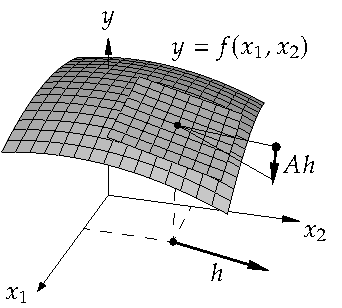
\includegraphics{figures/svder}
\caption{Illustration of a derivative for a function $f \colon \R^2 \to \R$.  The vector $h$ is shown
in the $x_1x_2$-plane based at $(x_1,x_2)$, and the vector
$Ah \in \R^1$ is shown along the $y$ direction.\label{fig:svder}}
\end{myfigureht}

For a differentiable function,
the derivative of $f$ is a function from $U$ to $L(\R^n,\R^m)$.  Compare
to the one-dimensional case, where the derivative is a function
from $U$ to $\R$, but we really want to think of $\R$ here as
$L(\R^1,\R^1)$.  As in one dimension, the idea is that a differentiable
mapping is \myquote{infinitesimally close} to a linear mapping, and this
linear mapping is the derivative.

Notice which norms are being used in the definition.
The norm in the
numerator is on $\R^m$, and the norm in the denominator is on $\R^n$ where $h$
lives.
Normally it is understood that $h \in \R^n$ from context
(the formula makes no sense otherwise).
We will not explicitly say so from now on.

We have again cheated somewhat and said that $A$
is \emph{the} derivative.  We have not shown yet that there
is only one, let us do that now.

\begin{prop}
Let $U \subset \R^n$ be an open subset and $f \colon U \to \R^m$ a function.  Suppose
$x \in U$ and there exist 
$A,B \in L(\R^n,\R^m)$ such that
\begin{equation*}
\lim_{h \to 0}
\frac{\snorm{f(x+h)-f(x) - Ah}}{\snorm{h}} = 0
\qquad \text{and} \qquad
\lim_{h \to 0}
\frac{\snorm{f(x+h)-f(x) - Bh}}{\snorm{h}} = 0 .
\end{equation*}
Then $A=B$.
\end{prop}

\begin{proof}
Suppose $h \in \R^n$, $h \not= 0$.  Compute
\begin{equation*}
\begin{split}
\frac{\snorm{(A-B)h}}{\snorm{h}} & =
\frac{\snorm{f(x+h)-f(x) - Ah - (f(x+h)-f(x) - Bh)}}{\snorm{h}} \\
& \leq
\frac{\snorm{f(x+h)-f(x) - Ah}}{\snorm{h}} + \frac{\snorm{f(x+h)-f(x) -
Bh}}{\snorm{h}} .
\end{split}
\end{equation*}
So 
$\frac{\snorm{(A-B)h}}{\snorm{h}} \to 0$ as $h \to 0$.  That is, given
$\epsilon > 0$, then for all nonzero $h$ in some $\delta$-ball around
the origin
\begin{equation*}
\epsilon > 
\frac{\snorm{(A-B)h}}{\snorm{h}}
=
\norm{(A-B)\frac{h}{\snorm{h}}} .
\end{equation*}
For any given $x$ with $\snorm{x}=1$,
let $h = (\nicefrac{\delta}{2}) \, x$, then $\snorm{h} < \delta$
and $\frac{h}{\snorm{h}} = x$.
So $\snorm{(A-B)x} < \epsilon$.  Taking the supremum over all $x$ with
$\snorm{x} = 1$, we get the operator norm
$\snorm{A-B} \leq \epsilon$.  As $\epsilon > 0$
was arbitrary, $\snorm{A-B} = 0$, or in other words $A = B$.
\end{proof}

\begin{example}
If $f(x) = Ax$ for a linear mapping $A$, then
$f'(x) = A$:
\begin{equation*}
\frac{\snorm{f(x+h)-f(x) - Ah}}{\snorm{h}}
=
\frac{\snorm{A(x+h)-Ax - Ah}}{\snorm{h}}
=
\frac{0}{\snorm{h}} = 0 .
\end{equation*}
\end{example}

\begin{example}
Let $f \colon \R^2 \to \R^2$ be defined by
\begin{equation*}
f(x,y) = \bigl(f_1(x,y),f_2(x,y)\bigr) := (1+x+2y+x^2,2x+3y+xy).
\end{equation*}
Let us show that $f$ is differentiable at the origin and let us 
compute the derivative,
directly using the definition.  If the
derivative exists, it is in $L(\R^2,\R^2)$, so it can be
represented by a $2$-by-$2$ matrix
$\left[\begin{smallmatrix}a&b\\c&d\end{smallmatrix}\right]$.  Suppose $h =
(h_1,h_2)$.  We need the following expression to go to zero.
\begin{multline*}
\frac{\snorm{
f(h_1,h_2)-f(0,0)
-
(ah_1 +bh_2 , ch_1+dh_2)}
}{\snorm{(h_1,h_2)}}
=
\\
\frac{\sqrt{
{\bigl((1-a)h_1 + (2-b)h_2 + h_1^2\bigr)}^2
+
{\bigl((2-c)h_1 + (3-d)h_2 + h_1h_2\bigr)}^2}}{\sqrt{h_1^2+h_2^2}} .
\end{multline*}
If we choose $a=1$, $b=2$, $c=2$, $d=3$, the expression becomes
\begin{equation*}
\frac{\sqrt{
h_1^4 + h_1^2h_2^2}}{\sqrt{h_1^2+h_2^2}}
=
\sabs{h_1}
\frac{\sqrt{
h_1^2 + h_2^2}}{\sqrt{h_1^2+h_2^2}}
= \sabs{h_1} .
\end{equation*}
This expression does indeed go to zero as $h \to 0$.  The
function $f$ is differentiable at the origin and 
the derivative $f'(0)$ is represented by the matrix
$\left[\begin{smallmatrix}1&2\\2&3\end{smallmatrix}\right]$.
\end{example}

\begin{prop}
Let $U \subset \R^n$ be open and $f \colon U \to \R^m$ be
differentiable at $p \in U$.  Then $f$ is continuous at $p$.
\end{prop}

\begin{proof}
Another way to write the differentiability of $f$ at $p$ is to consider
\begin{equation*}
r(h) := f(p+h)-f(p) - f'(p) h .
\end{equation*}
The function $f$ is differentiable at $p$ if
$\frac{\snorm{r(h)}}{\snorm{h}}$ goes to zero as $h \to 0$,
so
$r(h)$ itself goes to zero.  The mapping $h \mapsto f'(p) h$
is a linear mapping between finite-dimensional spaces, hence continuous
and $f'(p) h \to 0$ as $h \to 0$.  Thus,
$f(p+h)$ must go to $f(p)$ as $h \to 0$.  That is, $f$ is continuous at $p$.
\end{proof}

The derivative is itself a linear operator on the space of differentiable
functions.

\begin{prop}
Suppose $U \subset \R^n$ is open,
$f \colon U \to \R^m$ and
$g \colon U \to \R^m$ are differentiable at $p$,
and $\alpha \in \R$.  Then the functions $f+g$ and $\alpha f$
are differentiable at $p$ and
\begin{equation*}
(f+g)'(p) = f'(p) + g'(p) , \qquad \text{and} \qquad (\alpha f)'(p) = \alpha
f'(p) .
\end{equation*}
\end{prop}

\begin{proof}
Let $h \in \R^n$, $h \not= 0$.  Then
\begin{multline*}
\frac{\norm{f(p+h)+g(p+h)-\bigl(f(p)+g(p)\bigr) - \bigl(f'(p) + g'(p)\bigr)h}}{\snorm{h}}
\\
\leq
\frac{\norm{f(p+h)-f(p) - f'(p)h}}{\snorm{h}}
+
\frac{\norm{g(p+h)-g(p) - g'(p)h}}{\snorm{h}} ,
\end{multline*}
and
\begin{equation*}
\frac{\norm{\alpha f(p+h) - \alpha f(p) - \alpha f'(p)h}}{\snorm{h}}
=
\sabs{\alpha} \frac{\norm{f(p+h))-f(p) - f'(p)h}}{\snorm{h}} .
\end{equation*}
The limits as $h$ goes to zero of the right-hand sides are zero by
hypothesis.  The result follows.
\end{proof}

If $A \in L(X,Y)$ and $B \in L(Y,Z)$ are linear maps, then 
they are their own derivative.  The composition
$BA \in L(X,Z)$ is also its own derivative, and
so the derivative of the composition is the composition
of the derivatives.  As differentiable maps are
\myquote{infinitesimally close}
to linear maps, they have the same property:

\begin{thm}[Chain rule] \index{chain rule}
Let $U \subset \R^n$ be open and let $f \colon U \to \R^m$ be
differentiable at $p \in U$.  Let $V \subset \R^m$ be open,
$f(U) \subset V$ and let $g \colon V \to \R^\ell$ be differentiable
at $f(p)$.  Then
\begin{equation*}
F(x) = g\bigl(f(x)\bigr)
\end{equation*}
is differentiable at $p$ and
\begin{equation*}
F'(p) = g'\bigl(f(p)\bigr) f'(p) .
\end{equation*}
\end{thm}

Without the points where things are evaluated, this is sometimes written as
$F' = {(g \circ f)}' = g' f'$.  The way to
understand it is that the derivative of the composition $g \circ f$
is the composition of the derivatives of $g$ and $f$.  If
$f'(p) = A$ and $g'\bigl(f(p)\bigr) = B$, then $F'(p) = BA$,
just as for linear maps.

\begin{proof}
Let $A := f'(p)$ and $B := g'\bigl(f(p)\bigr)$.  Take a nonzero $h \in \R^n$
and write $q = f(p)$, $k = f(p+h)-f(p)$.  Let
\begin{equation*}
r(h) := f(p+h)-f(p) - A h . %= k - Ah.
\end{equation*}
Then $r(h) = k-Ah$ or $Ah = k-r(h)$, and $f(p+h) = q+k$.
We look at the quantity we need to go
to zero:
\begin{equation*}
\begin{split}
\frac{\snorm{F(p+h)-F(p) - BAh}}{\snorm{h}}
& =
\frac{\snorm{g\bigl(f(p+h)\bigr)-g\bigl(f(p)\bigr) - BAh}}{\snorm{h}}
\\
& =
\frac{\snorm{g(q+k)-g(q) - B\bigl(k-r(h)\bigr)}}{\snorm{h}}
\\
& \leq
\frac
{\snorm{g(q+k)-g(q) - Bk}}
{\snorm{h}}
+
\snorm{B}
\frac
{\snorm{r(h)}}
{\snorm{h}}
\\
& =
\frac
{\snorm{g(q+k)-g(q) - Bk}}
{\snorm{k}}
\frac
{\snorm{f(p+h)-f(p)}}
{\snorm{h}}
+
\snorm{B}
\frac
{\snorm{r(h)}}
{\snorm{h}} .
\end{split}
\end{equation*}
First, $\snorm{B}$ is a constant and $f$ is differentiable at $p$,
so
the term $\snorm{B}\frac{\snorm{r(h)}}{\snorm{h}}$ goes to 0.
Next because $f$ is continuous at $p$, then as
$h$ goes to 0, so $k$ goes to 0.  Thus
$\frac
{\snorm{g(q+k)-g(q) - Bk}}
{\snorm{k}}$ goes to 0, because $g$ is differentiable at $q$.
Finally,
\begin{equation*}
\frac
{\snorm{f(p+h)-f(p)}}
{\snorm{h}}
\leq
\frac
{\snorm{f(p+h)-f(p)-Ah}}
{\snorm{h}}
+
\frac
{\snorm{Ah}}
{\snorm{h}}
\leq
\frac
{\snorm{f(p+h)-f(p)-Ah}}
{\snorm{h}}
+
\snorm{A} .
\end{equation*}
As $f$ is differentiable at $p$,
for small enough $h$, the quantity
$\frac{\snorm{f(p+h)-f(p)-Ah}}{\snorm{h}}$ is bounded.  Hence, the
term
$
\frac
{\snorm{f(p+h)-f(p)}}
{\snorm{h}}
$
stays bounded as $h$ goes to 0.  Therefore, 
$\frac{\snorm{F(p+h)-F(p) - BAh}}{\snorm{h}}$ goes to zero, and
$F'(p) = BA$, which is what was claimed.
\end{proof}

\subsection{Partial derivatives}

There is another way to generalize the derivative from one dimension.
We hold all but one variable constant and take the regular
derivative.

\begin{defn}
Let
$f \colon U \to \R$ be a function on an open set $U \subset \R^n$.
If the following limit exists, we write
\glsadd{not:partialder}
\begin{equation*}
\frac{\partial f}{\partial x_j} (x) := 
\lim_{h\to 0}\frac{f(x_1,\ldots,x_{j-1},x_j+h,x_{j+1},\ldots,x_n)-f(x)}{h}
=
\lim_{h\to 0}\frac{f(x+h e_j)-f(x)}{h} .
\end{equation*}
We call 
$\frac{\partial f}{\partial x_j} (x)$ the \emph{\myindex{partial derivative}}
of $f$
with respect to $x_j$.  %Sometimes we write $D_j f$ instead.
See \figureref{fig:svpartder}.
Here $h$ is a number not a vector.

For a mapping $f \colon U \to \R^m$ we write
$f = (f_1,f_2,\ldots,f_m)$, where $f_k$ are real-valued
functions.  We then take partial derivatives of
the components,
$\frac{\partial f_k}{\partial x_j}$.
\end{defn}

\begin{myfigureht}
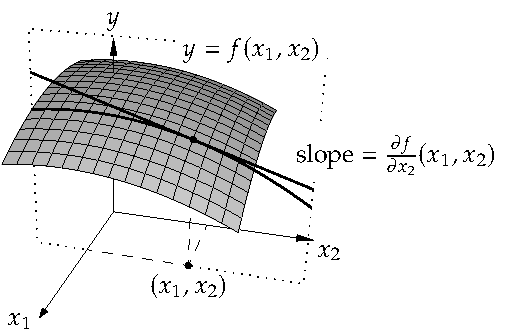
\includegraphics{figures/svpartder}
\caption{Illustration of a partial derivative for a function $f \colon \R^2
\to \R$.  The $yx_2$-plane where $x_1$ is fixed is marked in dotted line,
and the slope of the tangent line in the $yx_2$-plane is
$\frac{\partial f}{\partial x_2}(x_1,x_2)$.\label{fig:svpartder}}
\end{myfigureht}

Partial derivatives are easier to compute with all the machinery of
calculus, and they provide a way to compute the derivative of a
function.

\begin{prop} \label{mv:prop:jacobianmatrix}
Let $U \subset \R^n$ be open and let $f \colon U \to \R^m$ be
differentiable at $p \in U$.  Then all the partial derivatives at $p$
exist and, in terms of the standard bases of $\R^n$ and $\R^m$,
$f'(p)$ is represented by the matrix
\begin{equation*}
\begin{bmatrix}
\frac{\partial f_1}{\partial x_1}(p)
&
\frac{\partial f_1}{\partial x_2}(p)
& \ldots &
\frac{\partial f_1}{\partial x_n}(p)
\\[6pt]
\frac{\partial f_2}{\partial x_1}(p)
&
\frac{\partial f_2}{\partial x_2}(p)
& \ldots &
\frac{\partial f_2}{\partial x_n}(p)
\\
\vdots & \vdots & \ddots & \vdots
\\
\frac{\partial f_m}{\partial x_1}(p)
&
\frac{\partial f_m}{\partial x_2}(p)
& \ldots &
\frac{\partial f_m}{\partial x_n}(p)
\end{bmatrix} .
\end{equation*}
\end{prop}


In other words,
\begin{equation*}
f'(p) \, e_j =
\sum_{k=1}^m
\frac{\partial f_k}{\partial x_j}(p) \,e_k .
\end{equation*}
If $v = \sum_{j=1}^n c_j\, e_j = (c_1,c_2,\ldots,c_n)$, then
\begin{equation*}
f'(p) \, v =
\sum_{j=1}^n
\sum_{k=1}^m
 c_j
\frac{\partial f_k}{\partial x_j}(p) \,e_k
=
\sum_{k=1}^m
\left(
\sum_{j=1}^n
 c_j
\frac{\partial f_k}{\partial x_j}(p) \right) \,e_k .
\end{equation*}

\begin{proof}
Fix a $j$ and note that for nonzero $h$,
\begin{equation*}
\begin{split}
\norm{\frac{f(p+h e_j)-f(p)}{h} - f'(p) \, e_j} & = 
\norm{\frac{f(p+h e_j)-f(p) - f'(p) \, h e_j}{h}} \\
& =
\frac{\snorm{f(p+h e_j)-f(p) - f'(p) \, h e_j}}{\snorm{h e_j}} .
\end{split}
\end{equation*}
As $h$ goes to 0, the right-hand side goes to zero by
differentiability of $f$, and hence
\begin{equation*}
\lim_{h \to 0}
\frac{f(p+h e_j)-f(p)}{h} = f'(p) \, e_j  .
\end{equation*}
Let us represent $f$ by components
$f = (f_1,f_2,\ldots,f_m)$, since it is vector-valued.
Taking a limit in $\R^m$
is the same as taking the limit in each component separately.  
For every $k$,
the partial derivative
\begin{equation*}
\frac{\partial f_k}{\partial x_j} (p)
=
\lim_{h \to 0}
\frac{f_k(p+h e_j)-f_k(p)}{h}
\end{equation*}
exists and is equal to the $k$th component of $f'(p)\, e_j$,
and we are done.
\end{proof}

The converse of the proposition is not true.  Just because the partial
derivatives exist, does not mean that the function is differentiable.  See
the exercises.
However, when the partial derivatives are continuous, we will prove that the
converse holds.
One of the consequences of the proposition is that if $f$
is differentiable on $U$, then $f' \colon U \to
L(\R^n,\R^m)$ is a continuous function if and only if
all the $\frac{\partial f_k}{\partial x_j}$ are continuous functions.

\subsection{Gradients, curves, and directional derivatives}

Let $U \subset \R^n$ be open and $f \colon U \to \R$ a differentiable
function.  We define
the \emph{\myindex{gradient}} as
\glsadd{not:gradient}
\begin{equation*}
\nabla f (x) := \sum_{j=1}^n \frac{\partial f}{\partial x_j} (x)\, e_j .
\end{equation*}
The gradient gives a way to represent the action of
the derivative as a dot product: $f'(x)\,v = \nabla f(x) \cdot v$.

Suppose $\gamma \colon (a,b) \subset \R \to \R^n$ is a differentiable
function.
Such a function and its image is sometimes called a \emph{\myindex{curve}},
or a \emph{\myindex{differentiable curve}}.
Write $\gamma =
(\gamma_1,\gamma_2,\ldots,\gamma_n)$.
For the purposes of computation
we identify $L(\R^1)$ and $\R$ as we did when we defined the
derivative in one variable.
We also identify $L(\R^1,\R^n)$ with $\R^n$.
We treat $\gamma^{\:\prime}(t)$ both as an operator in
$L(\R^1,\R^n)$ and the vector
$\bigl(\gamma_1^{\:\prime}(t),
\gamma_2^{\:\prime}(t),\ldots,\gamma_n^{\:\prime}(t)\bigr)$
in $\R^n$.
Using \propref{mv:prop:jacobianmatrix},
if $v\in \R^n$ is $\gamma^{\:\prime}(t)$ acting as a vector,
then $h \mapsto h \, v$ (for $h \in \R^1 = \R$) is
$\gamma^{\:\prime}(t)$ acting as an operator
in $L(\R^1,\R^n)$.
We often use this 
slight abuse of notation when dealing with curves.
See \figureref{fig:difcurveder}.
\begin{myfigureht}
\subimport*{figures/}{diffcurveder.pdf_t}
\caption{Differentiable curve and its derivative as a
vector.\label{fig:difcurveder}}
\end{myfigureht}

Suppose $\gamma\bigl((a,b)\bigr) \subset U$ and let
\begin{equation*}
g(t) := f\bigl(\gamma(t)\bigr) .
\end{equation*}
The function
$g$ is differentiable. Treating $g'(t)$ as a number,
\begin{equation*}
g'(t) =
f'\bigl(\gamma(t)\bigr) \gamma^{\:\prime}(t)
=
\sum_{j=1}^n
\frac{\partial f}{\partial x_j} \bigl(\gamma(t)\bigr)
\frac{d\gamma_j}{dt} (t)
=
\sum_{j=1}^n
\frac{\partial f}{\partial x_j}
\frac{d\gamma_j}{dt} .
\end{equation*}
For convenience,
we often 
leave out the points where we are evaluating,
such as above on the far right-hand side.
With the notation of the gradient and the dot product
the equation becomes
\begin{equation*}
g'(t) = (\nabla f) \bigl(\gamma(t)\bigr) \cdot \gamma^{\:\prime}(t)
= \nabla f \cdot \gamma^{\:\prime}.
\end{equation*}

We use this idea to define derivatives in a specific direction.  A direction
is simply a vector pointing in that direction.  Pick a vector $u \in \R^n$
such that $\snorm{u} = 1$, and fix $x \in U$.
We define the
\emph{\myindex{directional derivative}} as
\glsadd{not:mvdirder}
\begin{equation*}
D_u f (x) := \frac{d}{dt}\Big|_{t=0} \bigl[ f(x+tu) \bigr] =
\lim_{h\to 0}
\frac{f(x+hu)-f(x)}{h} ,
\end{equation*}
where the notation
$\frac{d}{dt}\big|_{t=0}$ represents the derivative evaluated at $t=0$.
Taking the standard basis vector $e_j$ we find
$\frac{\partial f}{\partial x_j} = D_{e_j} f$.
For this reason, sometimes the notation $\frac{\partial f}{\partial u}$
is used instead of $D_u f$.

Let $\gamma$ be defined by
\begin{equation*}
\gamma(t) := x + tu .
\end{equation*}
Then $\gamma^{\:\prime}(t) = u$ for all $t$.  
By the computation above:
\begin{equation*}
D_u f (x) =
\frac{d}{dt}\Big|_{t=0} \bigl[ f(x+tu) \bigr] =
(\nabla f) \bigl(\gamma(0)\bigr) \cdot \gamma^{\:\prime}(0)
=
(\nabla f) (x) \cdot u .
\end{equation*}

Suppose $(\nabla f)(x) \neq 0$.
By the Cauchy--Schwarz inequality,
\begin{equation*}
\sabs{D_u f(x)} \leq \snorm{(\nabla f)(x)} .
\end{equation*}
Equality is achieved when $u$ is a scalar multiple of
$(\nabla f)(x)$.  That is, when
\begin{equation*}
u = 
\frac{(\nabla f)(x)}{\snorm{(\nabla f)(x)}} ,
\end{equation*}
we get $D_u f(x) = \snorm{(\nabla f)(x)}$.
The gradient points in the direction in which the
function grows fastest, in other words,
in the direction in which $D_u f(x)$ is maximal.

\subsection{The Jacobian}

\begin{defn}
Let $U \subset \R^n$ and
$f \colon U \to \R^n$ be a differentiable mapping.  Define the
\emph{\myindex{Jacobian}}%
\footnote{Named after the Italian mathematician
\href{https://en.wikipedia.org/wiki/Carl_Gustav_Jacob_Jacobi}{Carl Gustav Jacob Jacobi}
(1804--1851).},
or the
\emph{\myindex{Jacobian determinant}}%
\footnote{The matrix from \propref{mv:prop:jacobianmatrix} representing $f'(x)$
is sometimes called the
\emph{\myindex{Jacobian matrix}}.},
of $f$ at $x$ as
\glsadd{not:jacobdet}
\begin{equation*}
J_f(x) := \det\bigl( f'(x) \bigr) .
\end{equation*}
Sometimes $J_f$ is written as
\begin{equation*}
\frac{\partial(f_1,f_2,\ldots,f_n)}{\partial(x_1,x_2,\ldots,x_n)} .
\end{equation*}
\end{defn}

This last piece of notation may seem somewhat confusing,
but it is quite useful when we need to specify
the exact variables and function components used,
as will for example do in the implicit function theorem.

The Jacobian $J_f$ is a real-valued function, and when $n=1$ it is simply the
derivative.
From the chain rule and the fact that $\det(AB) = \det(A)\det(B)$, it follows that:
\begin{equation*}
J_{f \circ g} (x) = J_f\bigl(g(x)\bigr) J_g(x) .
\end{equation*}

The determinant of a linear mapping tells us what happens to
area/volume under the mapping.
Similarly, the Jacobian measures how much a differentiable mapping stretches
things locally, and if it flips orientation.  In particular, if the Jacobian
is non-zero than we would assume that locally the mapping is invertible (and
we would be correct as we will later see).

\subsection{Exercises}

\begin{exercise}
Suppose $\gamma \colon (-1,1) \to \R^n$ and
$\alpha \colon (-1,1) \to \R^n$ are two differentiable curves
such that $\gamma(0) = \alpha(0)$ and $\gamma^{\:\prime}(0) = \alpha'(0)$.
Suppose $F \colon \R^n \to \R$ is a differentiable function.  Show that
\begin{equation*}
\frac{d}{dt}\Big|_{t=0}
F\bigl(\gamma(t)\bigr)
=
\frac{d}{dt}\Big|_{t=0}
F\bigl(\alpha(t)\bigr)
.
\end{equation*}
\end{exercise}

\begin{exercise}
Let $f \colon \R^2 \to \R$ be given by
$f(x,y)
:=
\sqrt{x^2+y^2}$,
see \figureref{fig:distfromorgfunc}.
Show that $f$ is not differentiable at the origin.
\end{exercise}

\begin{myfigureht}
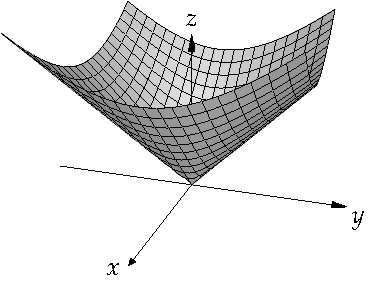
\includegraphics{figures/distfromorgfunc}
\caption{Graph of $\sqrt{x^2+y^2}$.\label{fig:distfromorgfunc}}
\end{myfigureht}

\begin{samepage}
\begin{exercise}
Using only the definition of the derivative, show that
the following $f \colon \R^2 \to \R^2$ are differentiable at the origin and
find their derivative.
\begin{enumerate}[a)]
\item
$f(x,y) := (1+x+xy,x)$,
\item
$f(x,y) := \bigl(y-y^{10},x \bigr)$,
\item
$f(x,y) := \bigl( {(x+y+1)}^2 , {(x-y+2)}^2 \bigr)$.
\end{enumerate}
\end{exercise}
\end{samepage}

\begin{exercise}
Suppose $f \colon \R \to \R$ and $g \colon \R \to \R$ are differentiable
functions.  Using only the definition of the derivative, show that
$h \colon \R^2 \to \R^2$ defined by $h(x,y)
:= \bigl(f(x),g(y)\bigr)$ is a differentiable function, and find the
derivative, at all points $(x,y)$.
\end{exercise}

\begin{exercise} \label{exercise:noncontpartialsexist}
Define a function $f \colon \R^2 \to \R$ by
(see \figureref{fig:xyxsqysqvol2})
\begin{equation*}
f(x,y)
:=
\begin{cases}
\frac{xy}{x^2+y^2} & \text{if } (x,y) \not= (0,0), \\
0                  & \text{if } (x,y) = (0,0).
\end{cases}
\end{equation*}
\begin{enumerate}[a)]
\item
Show that the partial derivatives 
$\frac{\partial f}{\partial x}$ and
$\frac{\partial f}{\partial y}$ exist at all points (including the origin).
\item
Show that $f$ is not continuous at the origin (and hence not
differentiable).
\end{enumerate}
\end{exercise}

\begin{myfigureht}
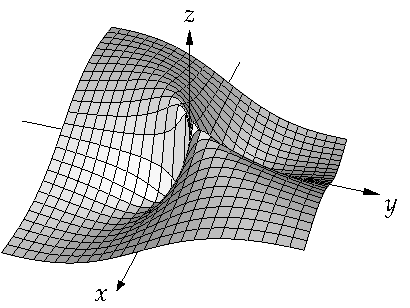
\includegraphics{figures/xyxsqysq}
\caption{Graph of $\frac{xy}{x^2+y^2}$.\label{fig:xyxsqysqvol2}}
\end{myfigureht}

\begin{samepage}
\begin{exercise}
Define a function $f \colon \R^2 \to \R$ by
(see \figureref{fig:xsqyxsqysq})
\begin{equation*}
f(x,y)
:=
\begin{cases}
\frac{x^2y}{x^2+y^2} & \text{if } (x,y) \not= (0,0), \\
0                    & \text{if } (x,y) = (0,0).
\end{cases}
\end{equation*}
\begin{enumerate}[a)]
\item
Show that the partial derivatives 
$\frac{\partial f}{\partial x}$ and
$\frac{\partial f}{\partial y}$ exist at all points.
\item
Show that for all $u \in \R^2$ with $\snorm{u}=1$, the directional
derivative $D_u f$ exists at all points.
\item
Show that $f$ is continuous at the origin.
\item
Show that $f$ is not differentiable at the origin.
\end{enumerate}
\end{exercise}
\end{samepage}

\begin{myfigureht}
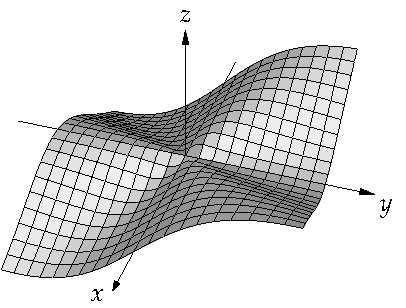
\includegraphics{figures/xsqyxsqysq}
\caption{Graph of $\frac{x^2y}{x^2+y^2}$.\label{fig:xsqyxsqysq}}
\end{myfigureht}

\begin{samepage}
\begin{exercise}
Suppose $f \colon \R^n \to \R^n$ is one-to-one, onto, differentiable at all
points, and such that $f^{-1}$ is also differentiable at all points.
\begin{enumerate}[a)]
\item
Show that $f'(p)$ is invertible at all points $p$ and compute
${(f^{-1})}'\bigl(f(p)\bigr)$.  Hint: Consider $x = f^{-1}\bigl(f(x)\bigr)$.
\item
Let $g \colon \R^n \to \R^n$ be a function differentiable at $q \in \R^n$
and such that $g(q)=q$.  Suppose $f(p) = q$ for some $p \in \R^n$.
Show $J_g(q) = J_{f^{-1} \circ g \circ f}(p)$ where $J_g$ is the Jacobian
determinant.
\end{enumerate}
\end{exercise}
\end{samepage}

\begin{exercise}
Suppose $f \colon \R^2 \to \R$ is differentiable and such that
$f(x,y) = 0$ if and only if $y=0$ and such that $\nabla f(0,0) = (0,1)$.
Prove that $f(x,y) > 0$ whenever $y > 0$, and
$f(x,y) < 0$ whenever $y < 0$.
\end{exercise}

\pagebreak[2]
\begin{exnote}
As for functions of one variable, $f \colon U \to \R$ has a
\emph{\myindex{relative maximum}} at $p \in U$ if there exists
a $\delta >0$ such that $f(q) \leq f(p)$ for all $q \in B(p,\delta) \cap U$.
Similarly for \emph{\myindex{relative minimum}}.
\end{exnote}

\begin{exercise} \label{exercise:mv:maximumcritical}
Suppose $U \subset \R^n$ is open and
$f \colon U \to \R$ is differentiable.  Suppose $f$ has a relative maximum
at $p \in U$.  Show that $f'(p) = 0$, that is the zero mapping in
$L(\R^n,\R)$.  That is $p$ is a
\emph{\myindex{critical point}} of $f$.
\end{exercise}

\begin{exercise}
Suppose $f \colon \R^2 \to \R$ is differentiable and 
$f(x,y) = 0$ whenever $x^2+y^2 = 1$.
Prove that there exists at least
one point $(x_0,y_0)$ such that
$\frac{\partial f}{\partial x}(x_0,y_0) = \frac{\partial f}{\partial
y}(x_0,y_0) = 0$.
\end{exercise}

\begin{exercise} \label{exercise:peano}
Define $f(x,y) := ( x-y^2 ) ( 2 y^2 - x)$.  The graph of $f$ is called
the \emph{\myindex{Peano surface}}.%
\footnote{Named after the Italian mathematician
\href{https://en.wikipedia.org/wiki/Giuseppe_Peano}{Giuseppe Peano}
(1858--1932).}
\begin{enumerate}[a)]
\item
Show that
$(0,0)$ is a critical point, that is $f'(0,0) = 0$, that is the zero
linear map in $L(\R^2,\R)$.
\item
Show that for every direction the restriction of $f$ to a line through the origin
in that direction has a relative maximum at the origin.  In other words,
for every $(x,y)$ such that $x^2+y^2=1$, the function $g(t) := f(tx,ty)$,
has a relative maximum at $t=0$.\\
Hint: While not necessary
\volIref{\sectionref*{vI-sec:taylor} of volume I}{\sectionref{sec:taylor}}
makes
this part easier.
\item
Show that $f$ does not have a relative maximum at $(0,0)$.
\end{enumerate}
\end{exercise}

\begin{exercise}
Suppose $f \colon \R \to \R^n$ is differentiable and $\snorm{f(t)} = 1$ for
all $t$ (that is, we have a curve in the unit sphere).  Show that 
$f'(t) \cdot f(t) = 0$ (treating $f'$ as a vector) for all $t$.
\end{exercise}

\begin{exercise}
Define $f \colon \R^2 \to \R^2$ by $f(x,y) :=
\bigl(x,y+\varphi(x)\bigr)$ for some differentiable function $\varphi$ of one
variable.  Show $f$ is differentiable and find $f'$.
\end{exercise}

\begin{exercise}
Suppose $U \subset \R^n$ is open, $p \in U$, and
$f \colon U \to \R$,
$g \colon U \to \R$,
$h \colon U \to \R$ are functions such that
$f(p) = g(p) = h(p)$, $f$ and $h$ are differentiable at $p$,
$f'(p) = h'(p)$, and
\begin{equation*}
f(x) \leq g(x) \leq h(x)
\end{equation*}
for all $x \in U$.  Show that $g$ is differentiable at $p$ and 
$g'(p) = f'(p) = h'(p)$.
\end{exercise}

%%%%%%%%%%%%%%%%%%%%%%%%%%%%%%%%%%%%%%%%%%%%%%%%%%%%%%%%%%%%%%%%%%%%%%%%%%%%%%

\sectionnewpage
\section{Continuity and the derivative}
\label{sec:svthedercont}

\sectionnotes{1--2 lectures}

\subsection{Bounding the derivative}

Let us prove a \myquote{mean value theorem} for vector-valued functions.

\begin{lemma} \label{lemma:mvtmv}
If $\varphi \colon [a,b] \to \R^n$ is differentiable on $(a,b)$ and
continuous on $[a,b]$, then there exists a $t_0 \in (a,b)$ such that
\begin{equation*}
\snorm{\varphi(b)-\varphi(a)} \leq (b-a) \snorm{\varphi'(t_0)} .
\end{equation*}
\end{lemma}

\begin{proof}
By the mean value theorem on the scalar-valued function
$t \mapsto \bigl(\varphi(b)-\varphi(a) \bigr) \cdot \varphi(t)$,
where the dot is the dot product, we obtain
that
there is a $t_0 \in (a,b)$ such that
\begin{equation*}
\begin{split}
\snorm{\varphi(b)-\varphi(a)}^2
& =
\bigl( \varphi(b)-\varphi(a) \bigr)
\cdot
\bigl( \varphi(b)-\varphi(a) \bigr)
\\
& =
\bigl(\varphi(b)-\varphi(a) \bigr) \cdot \varphi(b) - 
\bigl(\varphi(b)-\varphi(a) \bigr) \cdot \varphi(a)
\\
& = 
(b-a)
\bigl(\varphi(b)-\varphi(a) \bigr) \cdot \varphi'(t_0) ,
\end{split}
\end{equation*}
where we treat $\varphi'$ as a vector in $\R^n$ by the abuse of
notation we mentioned in the previous section.
If we think of $\varphi'(t)$ as a vector, then by
\exerciseref{exercise:normonedim},
$\snorm{\varphi'(t)}_{L(\R,\R^n)} = \snorm{\varphi'(t)}_{\R^n}$.
That is, the euclidean norm of the vector is the same as the operator norm
of $\varphi'(t)$.

By the Cauchy--Schwarz inequality
\begin{equation*}
\snorm{\varphi(b)-\varphi(a)}^2
=
(b-a)\bigl(\varphi(b)-\varphi(a) \bigr) \cdot \varphi'(t_0)
\leq
(b-a)
\snorm{\varphi(b)-\varphi(a)} \, \snorm{\varphi'(t_0)} . \qedhere
\end{equation*}
\end{proof}

Recall that a set $U$ is convex
if whenever $x,y \in U$, the line segment from
$x$ to $y$ lies in $U$.

\begin{prop} \label{mv:prop:convexlip}
Let $U \subset \R^n$ be a convex open set, $f \colon U \to \R^m$
be a differentiable function, and an $M$ be such that
\begin{equation*}
\snorm{f'(x)} \leq M
\qquad \text{for all } x \in U.
\end{equation*}
Then $f$ is Lipschitz with constant $M$, that is
\begin{equation*}
\snorm{f(x)-f(y)} \leq M \snorm{x-y}
\qquad
\text{for all } x,y \in U.
\end{equation*}
\end{prop}

\begin{proof}
Fix $x$ and $y$ in $U$ and note that
$(1-t)x+ty \in U$ for all $t \in [0,1]$
by convexity.
Next
\begin{equation*}
\frac{d}{dt} \Bigl[f\bigl((1-t)x+ty\bigr)\Bigr]
=
f'\bigl((1-t)x+ty\bigr) (y-x) .
\end{equation*}
By \lemmaref{lemma:mvtmv} there is some
$t_0 \in (0,1)$ such that
\begin{equation*}
\begin{split}
\snorm{f(x)-f(y)} & \leq
\norm{\frac{d}{dt} \Big|_{t=t_0} \Bigl[ f\bigl((1-t)x+ty\bigr) \Bigr] }
\\
& \leq
\norm{f'\bigl((1-t_0)x+t_0y\bigr)} \, \snorm{y-x} \leq
M \snorm{y-x} . \qedhere
\end{split}
\end{equation*}
\end{proof}

\begin{example}
If $U$ is not convex the proposition is not true: Consider
the set
\begin{equation*}
U := \bigl\{ (x,y) : 0.5 < x^2+y^2 < 2 \bigr\} \setminus \bigl\{ (x,0) : x <
0 \bigr\} .
\end{equation*}
For $(x,y) \in U$,
let $f(x,y)$ be the angle that the line from the origin to $(x,y)$
makes with the positive $x$ axis.  We even have a formula for $f$:
\begin{equation*}
f(x,y) = 2 \operatorname{arctan}\left( \frac{y}{x+\sqrt{x^2+y^2}}\right) .
\end{equation*}
Think a spiral staircase with room in the middle.  See
\figureref{mv:fignonlip}.

\begin{myfigureht}
\subimport*{figures/}{nonlip_full.pdf_t}
\caption{A non-Lipschitz function with uniformly bounded
derivative.\label{mv:fignonlip}}
\end{myfigureht}

The function is differentiable,
and the derivative is bounded on $U$, which is not hard to see.   Now
think of
what happens near where the negative $x$-axis cuts the annulus in half.
As we approach this cut from positive $y$, $f(x,y)$ approaches $\pi$.
From negative $y$, $f(x,y)$ approaches $-\pi$.
So for small $\epsilon > 0$, $\sabs{f(-1,\epsilon)-f(-1,-\epsilon)}$
approaches $2\pi$, but $\snorm{(-1,\epsilon)-(-1,-\epsilon)} = 2\epsilon$,
which is arbitrarily small.  The conclusion of the proposition does not
hold for this nonconvex $U$.
\end{example}

Let us solve the differential equation $f' = 0$.

\begin{cor}
If $U \subset \R^n$ is open and connected, $f \colon U \to \R^m$ is
differentiable,
and $f'(x) = 0$ for all $x \in U$, then $f$ is constant.
\end{cor}

\begin{proof}
For any given $x \in U$, there is a ball $B(x,\delta) \subset U$.  The ball
$B(x,\delta)$ is convex.  Since
$\snorm{f'(y)} \leq 0$ for all $y \in B(x,\delta)$, then by the proposition,
$\snorm{f(x)-f(y)} \leq 0 \snorm{x-y} = 0$.  So $f(x) = f(y)$ for all $y \in
B(x,\delta)$.

This means that $f^{-1}(c)$ is open for all $c \in \R^m$.  Suppose
$f^{-1}(c)$ is nonempty.  
The two sets
\begin{equation*}
U' = f^{-1}(c), \qquad U'' = f^{-1}\bigl(\R^m\setminus\{c\}\bigr)
\end{equation*}
are open and disjoint, and further $U = U' \cup U''$.  As $U'$ is nonempty
and $U$ is connected, then
$U'' = \emptyset$.  So $f(x) = c$ for all $x \in U$.
\end{proof}

\subsection{Continuously differentiable functions}

\begin{defn}
Let $U \subset \R^n$ be open.
We say $f \colon U \to \R^m$ is
\emph{\myindex{continuously differentiable}},
or $C^1(U)$\glsadd{not:C1},
if $f$ is differentiable and $f' \colon U \to L(\R^n,\R^m)$
is continuous.
\end{defn}

\begin{prop} \label{mv:prop:contdiffpartials}
Let $U \subset \R^n$ be open and
$f \colon U \to \R^m$.  The function
$f$ is continuously differentiable if and only if 
the partial derivatives $\frac{\partial f_j}{\partial x_\ell}$
exist for all $j$ and $\ell$ and are continuous.
\end{prop}

Without continuity the theorem does not hold.  Just because
partial derivatives exist does not mean that $f$ is differentiable,
in fact, $f$ may not even be continuous.  See the exercises
for the last section and also for this section.

\begin{proof}
We proved that if $f$ is differentiable, then
the partial derivatives exist.  The partial
derivatives are the entries of the matrix of $f'(x)$.  If
$f' \colon U \to L(\R^n,\R^m)$ is continuous, then the entries are
continuous, and hence the partial derivatives are continuous.

To prove the opposite direction,
suppose the partial derivatives exist and are continuous.
Fix $x \in U$.  If we show that $f'(x)$ exists we are done, because
the entries of the matrix $f'(x)$ are the partial derivatives and if
the entries are continuous functions, the matrix-valued function $f'$ is
continuous.

We do induction on dimension.  First,
the conclusion is true when $n=1$.  In this case the derivative
is just the regular derivative (exercise, noting
that $f$ is vector-valued).

Suppose the conclusion is true for $\R^{n-1}$,
that is,
if we restrict to the first $n-1$ variables, the function is differentiable.
It is easy to see that the first $n-1$
partial derivatives of $f$ restricted to the set where the last coordinate is
fixed are the same as those for $f$.
In the following, by a slight abuse of notation,
we think of $\R^{n-1}$ as a subset of $\R^n$, that is the set in $\R^n$ where $x_n = 0$.
In other words, we identify the vectors $(x_1,x_2,\ldots,x_{n-1})$ and
$(x_1,x_2,\ldots,x_{n-1},0)$.
Let
\begin{equation*}
A := 
\begin{bmatrix}
\frac{\partial f_1}{\partial x_1}(x)
& \ldots &
\frac{\partial f_1}{\partial x_n}(x)
\\
\vdots & \ddots & \vdots
\\
\frac{\partial f_m}{\partial x_1}(x)
& \ldots &
\frac{\partial f_m}{\partial x_n}(x)
\end{bmatrix} ,
\qquad
A' := 
\begin{bmatrix}
\frac{\partial f_1}{\partial x_1}(x)
& \ldots &
\frac{\partial f_1}{\partial x_{n-1}}(x)
\\
\vdots & \ddots & \vdots
\\
\frac{\partial f_m}{\partial x_1}(x)
& \ldots &
\frac{\partial f_m}{\partial x_{n-1}}(x)
\end{bmatrix} ,
\qquad
v := 
\begin{bmatrix}
\frac{\partial f_1}{\partial x_n}(x)
\\
\vdots
\\
\frac{\partial f_m}{\partial x_n}(x)
\end{bmatrix} .
\end{equation*}
Let $\epsilon > 0$ be given.  By the induction hypothesis, there
is a $\delta > 0$ such that
for every $k \in \R^{n-1}$ with $\snorm{k} < \delta$, we have
\begin{equation*}
\frac{\snorm{f(x+k) - f(x) - A' k}}{\snorm{k}} < \epsilon .
\end{equation*}
By continuity of the partial derivatives, suppose $\delta$ is small
enough so that
\begin{equation*}
\abs{\frac{\partial f_j}{\partial x_n}(x+h)
      - \frac{\partial f_j}{\partial x_n}(x)} < \epsilon
\end{equation*}
for all $j$ and all $h \in \R^n$ with $\snorm{h} < \delta$.

Suppose $h = k + t e_n$ is a vector in $\R^n$, where $k \in \R^{n-1}$, $t
\in \R$, such that
$\snorm{h} < \delta$.  Then $\snorm{k} \leq \snorm{h} < \delta$.
Note that $Ah = A' k + tv$.
\begin{equation*}
\begin{split}
\snorm{f(x+h) - f(x) - Ah}
& = \snorm{f(x+k + t e_n) - f(x+k) - tv + f(x+k) - f(x) - A' k}
\\
& \leq \snorm{f(x+k + t e_n) - f(x+k) -tv} + \snorm{f(x+k) - f(x) -
A' k}
\\
& \leq \snorm{f(x+k + t e_n) - f(x+k) -tv} + \epsilon \snorm{k} .
\end{split}
\end{equation*}
As all the partial derivatives exist, by the mean value theorem,
for each $j$ there is some $\theta_j \in [0,t]$ (or $[t,0]$ if $t < 0$), such that
\begin{equation*}
f_j(x+k + t e_n) - f_j(x+k) =
t \frac{\partial f_j}{\partial x_n}(x+k+\theta_j e_n).
\end{equation*}
Note that if $\snorm{h} < \delta$, then $\snorm{k+\theta_j e_n} \leq \snorm{h}
< \delta$.
We finish the estimate
\begin{equation*}
\begin{split}
\snorm{f(x+h) - f(x) - Ah}
& \leq \snorm{f(x+k + t e_n) - f(x+k) -tv} + \epsilon \snorm{k}
\\
& \leq \sqrt{\sum_{j=1}^m {\left(t\frac{\partial f_j}{\partial
x_n}(x+k+\theta_j e_n) -
t \frac{\partial f_j}{\partial x_n}(x)\right)}^2} + \epsilon \snorm{k}
\\
& \leq \sqrt{m}\, \epsilon \sabs{t} + \epsilon \snorm{k}
\\
& \leq (\sqrt{m}+1)\epsilon \snorm{h} . \qedhere
\end{split}
\end{equation*}
\end{proof}

A common application is to prove that a certain function is
differentiable.  For example, let us show that all polynomials
are differentiable, and in fact continuously differentiable
by computing the partial derivatives.

\begin{cor}
A polynomial $p \colon \R^n \to \R$ in several variables
\begin{equation*}
p(x_1,x_2,\ldots,x_n)
=
\sum_{0 \leq j_1+j_2+\cdots+j_n \leq d}
c_{j_1,j_2,\ldots,j_n}
\,
x_1^{j_1}
x_2^{j_2}
\cdots
x_n^{j_n}
\end{equation*}
is continuously differentiable.
\end{cor}

\begin{proof}
Consider the partial derivative of $p$ in the $x_n$ variable.
Write $p$ as
\begin{equation*}
p(x) = \sum_{j=0}^d p_j(x_1,\ldots,x_{n-1}) \, x_n^j ,
\end{equation*}
where $p_j$ are polynomials in one less variable.
Then
\begin{equation*}
\frac{\partial p}{\partial x_n}(x)
= \sum_{j=1}^d p_j(x_1,\ldots,x_{n-1}) \, j x_n^{j-1} ,
\end{equation*}
which is again a polynomial.
So the partial derivatives of polynomials exist and are again polynomials.
By the continuity of algebraic operations, polynomials are continuous functions.
Therefore $p$ is continuously differentiable.
\end{proof}

\subsection{Exercises}

\begin{exercise}
Define $f \colon \R^2 \to \R$ as
\begin{equation*}
f(x,y) :=
\begin{cases}
(x^2+y^2)\sin\bigl({(x^2+y^2)}^{-1}\bigr) & \text{if } (x,y) \not= (0,0), \\
0                                         & \text{if } (x,y) = (0,0).
\end{cases}
\end{equation*}
Show that $f$ is differentiable at the origin, but that it is not 
continuously differentiable.
\\
Note: Feel free to use what you know about sine and cosine from calculus.
\end{exercise}

\begin{exercise}
Let $f \colon \R^2 \to \R$ be the function from
\exerciseref{exercise:noncontpartialsexist}, that is,
\begin{equation*}
f(x,y)
:=
\begin{cases}
\frac{xy}{x^2+y^2} & \text{if } (x,y) \not= (0,0), \\
0                  & \text{if } (x,y) = (0,0).
\end{cases}
\end{equation*}
Compute the partial derivatives 
$\frac{\partial f}{\partial x}$ and
$\frac{\partial f}{\partial y}$ at all points and show that these are not
continuous functions.
\end{exercise}

\begin{exercise}
Let $B(0,1) \subset \R^2$ be the unit ball (disc), that is, the set given by
$x^2 + y^2 < 1$.
Suppose $f \colon B(0,1) \to \R$ is a differentiable function
such that $\sabs{f(0,0)} \leq 1$,
and 
$\babs{\frac{\partial f}{\partial x}} \leq 1$ and
$\babs{\frac{\partial f}{\partial y}} \leq 1$ for all
points in $B(0,1)$.
\begin{enumerate}[a)]
\item
Find an $M \in \R$ such that $\snorm{f'(x,y)} \leq M$
for all $(x,y) \in
B(0,1)$.
\item
Find a $B \in \R$ such that
$\sabs{f(x,y)} \leq B$
for all $(x,y) \in
B(0,1)$.
\end{enumerate}
\end{exercise}

\begin{exercise}
Define $\varphi \colon [0,2\pi] \to \R^2$ by $\varphi(t) =
\bigl(\sin(t),\cos(t)\bigr)$.  Compute $\varphi'(t)$ for all $t$.  Compute
$\snorm{\varphi'(t)}$ for all $t$.  Notice that $\varphi'(t)$ is never zero,
yet $\varphi(0) = \varphi(2\pi)$, therefore, Rolle's theorem is not true
in more than one dimension.
\end{exercise}

\begin{exercise}
Let $f \colon \R^2 \to \R$ be a function such that
$\frac{\partial f}{\partial x}$ and
$\frac{\partial f}{\partial y}$ exist at all points and there exists an $M
\in \R$
such that 
$\babs{\frac{\partial f}{\partial x}} \leq M$ and
$\babs{\frac{\partial f}{\partial y}} \leq M$ at all points.  Show that $f$
is continuous.
\end{exercise}

\begin{samepage}
\begin{exercise}
Let $f \colon \R^2 \to \R$ be a function and
$M \in R$, such that
for every $(x,y) \in \R^2$, the function $g(t) := f(xt,yt)$ is
differentiable
and $\sabs{g'(t)} \leq M$.
\begin{enumerate}[a)]
\item
Show that $f$ is continuous at $(0,0)$.
\item
Find an example of such an $f$ that is discontinuous at every other point of
$\R^2$.\\
Hint: Think back to how we constructed a nowhere continuous function on $[0,1]$.
\end{enumerate}
\end{exercise}
\end{samepage}

\begin{exercise}
Suppose $r \colon \R^n \setminus X \to \R$ is a rational function, that is,
let $p \colon \R^n \to \R$ and
$q \colon \R^n \to \R$ be polynomials,
$q$ not identically zero,
where $X = q^{-1}(0)$, and
$r = \frac{p}{q}$.
Show that $r$ is continuously differentiable.
\end{exercise}

\begin{exercise}
Suppose $f \colon \R^n \to \R$ and $h \colon \R^n \to \R$ are two 
differentiable functions such that $f'(x) = h'(x)$ for all $x \in \R^n$.
Prove that
if $f(0) = h(0)$, then $f(x) = h(x)$ for all $x \in \R^n$.
\end{exercise}

\begin{exercise}
Prove the base case
in \propref{mv:prop:contdiffpartials}.  That is, prove that
if $n=1$ and 
\myquote{the partials exist and are continuous,} then the function is continuously
differentiable.  Note that $f$ is vector-valued.
\end{exercise}

\begin{exercise}
Suppose $g \colon \R \to \R$ is continuously differentiable and
$h \colon \R^2 \to \R$ is continuous.  Show that
\begin{equation*}
F(x,y) := g(x) + \int_0^y h(x,s) ~ds
\end{equation*}
is continuously differentiable, and that it is the solution of 
the partial differential equation $\frac{\partial F}{\partial y} = h$,
with the initial condition $F(x,0) = g(x)$ for all $x \in \R$.
\end{exercise}


%%%%%%%%%%%%%%%%%%%%%%%%%%%%%%%%%%%%%%%%%%%%%%%%%%%%%%%%%%%%%%%%%%%%%%%%%%%%%%

\sectionnewpage
\section{Inverse and implicit function theorems}
\label{sec:svinvfuncthm}

\sectionnotes{2--3 lectures}

To prove the inverse function theorem we use the contraction mapping
principle from
\volIref{\chapterref*{vI-ms:chapter}}{\chapterref{ms:chapter}},
where we we used it
to prove Picard's theorem.
Recall that a mapping $f \colon X \to Y$ between two metric
spaces $(X,d_X)$ and $(Y,d_Y)$ is called a contraction 
if there exists a $k < 1$ such that
\begin{equation*}
d_Y\bigl(f(p),f(q)\bigr) \leq k \, d_X(p,q)
\qquad \text{for all } p,q \in X.
\end{equation*}
The contraction mapping principle says that if $f \colon X \to X$
is a contraction and $X$ is a complete metric space,
then there exists a unique fixed point, that is,
there exists a unique $x \in X$ such that $f(x) = x$.

Intuitively, if a function is continuously differentiable, then it
locally \myquote{behaves like} the derivative (which is a linear function).
The idea of the inverse function theorem is that if a function is
continuously differentiable and the derivative is invertible, the function is
(locally) invertible.


\begin{thm}[Inverse function theorem]\index{inverse function theorem}
\label{thm:inverse}
Let $U \subset \R^n$ be an open set and let
$f \colon U \to \R^n$ be a continuously differentiable function.
Suppose $p \in U$ and $f'(p)$ is invertible
(that is, $J_f(p) \not=0$).
Then there exist open sets $V, W \subset \R^n$ such that
$p \in V \subset U$, $f(V) = W$ and $f|_V$ is one-to-one.  
Hence a function $g \colon W \to V$ exists such that
$g(y) := (f|_V)^{-1}(y)$.
See \figureref{fig:inversefuncRn}.
Furthermore, $g$ is continuously differentiable
and 
\begin{equation*}
g'(y) = {\bigl(f'(x)\bigr)}^{-1}, \qquad \text{for all } x \in V, y = f(x).
\end{equation*}
\end{thm}

\begin{myfigureht}
\subimport*{figures/}{inversefuncRn.pdf_t}
\caption{Setup of the inverse function theorem in $\R^n$.\label{fig:inversefuncRn}}
\end{myfigureht}

\begin{proof}
Write $A = f'(p)$.  As $f'$ is continuous, there exists an open ball
$V$ around $p$ such that
\begin{equation*}
\snorm{A-f'(x)} < \frac{1}{2\snorm{A^{-1}}}
\qquad \text{for all } x \in V.
\end{equation*}
Consequently, the derivative $f'(x)$ is invertible for all $x \in V$
by \propref{prop:finitedimpropinv}.

Given $y \in \R^n$, we define $\varphi_y \colon V \to \R^n$ by
\begin{equation*}
\varphi_y (x) := x + A^{-1}\bigl(y-f(x)\bigr) .
\end{equation*}
As $A^{-1}$ is one-to-one,
$\varphi_y(x) = x$ ($x$ is a fixed point) if only if
$y-f(x) = 0$, or in other words $f(x)=y$.  Using the chain rule we obtain
\begin{equation*}
\varphi_y'(x) = I - A^{-1} f'(x) = A^{-1} \bigl( A-f'(x) \bigr) .
\end{equation*}
So for $x \in V$, we have
\begin{equation*}
\snorm{\varphi_y'(x)} \leq \snorm{A^{-1}} \, \snorm{A-f'(x)} < \nicefrac{1}{2} .
\end{equation*}
As $V$ is a ball, it is convex.  Hence
\begin{equation*}
\snorm{\varphi_y(x_1)-\varphi_y(x_2)} \leq \frac{1}{2} \snorm{x_1-x_2} 
\qquad
\text{for all } x_1,x_2 \in V.
\end{equation*}
In other words, $\varphi_y$ is a contraction defined on $V$, though we so far
do not know what is the range of $\varphi_y$.  We cannot yet
apply the fixed
point theorem, but we can say that $\varphi_y$ 
has at most one fixed point in $V$:
If $\varphi_y(x_1) = x_1$ and
$\varphi_y(x_2) = x_2$, then
$\snorm{x_1-x_2} = \snorm{\varphi_y(x_1)-\varphi_y(x_2)} \leq
\frac{1}{2} \snorm{x_1-x_2}$, so $x_1 = x_2$.
That is, there exists at most one $x \in V$
such that $f(x) = y$, and so $f|_V$ is one-to-one.

Let $W := f(V)$.  We need to show that $W$ is open.  Take a $y_0 \in W$.
There is a unique $x_0 \in V$ such that $f(x_0) = y_0$.
Let $r > 0$ be small enough such that the closed ball $C(x_0,r) \subset V$
(such $r > 0$ exists as $V$ is open).

Suppose $y$ is such that
\begin{equation*}
\snorm{y-y_0} <
\frac{r}{2\snorm{A^{-1}}} .
\end{equation*}
If we show that $y \in W$, then we have shown that $W$ is open.
If $x \in
C(x_0,r)$, then
\begin{equation*}
\begin{split}
\snorm{\varphi_y(x)-x_0}
& \leq
\snorm{\varphi_y(x)-\varphi_y(x_0)} +
\snorm{\varphi_y(x_0)-x_0} \\
& \leq
\frac{1}{2}\snorm{x-x_0} +
\snorm{A^{-1}(y-y_0)} \\
& \leq
\frac{1}{2}r +
\snorm{A^{-1}} \, \snorm{y-y_0} \\
& <
\frac{1}{2}r +
\snorm{A^{-1}}
\frac{r}{2\snorm{A^{-1}}} = r .
\end{split}
\end{equation*}
So $\varphi_y$ takes $C(x_0,r)$ into $B(x_0,r) \subset C(x_0,r)$.  It is a
contraction on $C(x_0,r)$ and $C(x_0,r)$ is complete (closed subset of $\R^n$
is complete).
Apply the contraction mapping principle to obtain a fixed point $x$,
i.e.\ $\varphi_y(x) = x$.  That is, $f(x) = y$, and $y \in
f\bigl(C(x_0,r)\bigr) \subset f(V) = W$.  Therefore $W$ is open.

Next we need to show that $g$ is continuously differentiable and compute
its derivative.  First let us show that it is differentiable.
Let $y \in W$ and $k \in \R^n$, $k\not= 0$, such that $y+k \in W$.
Because $f|_V$ is a one-to-one and onto mapping of $V$ onto $W$,
there are unique
$x \in V$ and $h \in \R^n$, $h \not= 0$ and $x+h \in V$, such that
$f(x) = y$ and $f(x+h) = y+k$.
In other words, $g(y) = x$ and $g(y+k) = x+h$.  See
\figureref{fig:inversefuncRn2}.
\begin{myfigureht}
\subimport*{figures/}{inversefuncRn2.pdf_t}
\caption{Proving that $g$ is differentiable.\label{fig:inversefuncRn2}}
\end{myfigureht}

We can still
squeeze some information from the fact that $\varphi_y$ is a contraction.
\begin{equation*}
\varphi_y(x+h)-\varphi_y(x) = h + A^{-1} \bigl( f(x)-f(x+h) \bigr) = h - A^{-1} k .
\end{equation*}
So
\begin{equation*}
\snorm{h-A^{-1}k} = \snorm{\varphi_y(x+h)-\varphi_y(x)} \leq
\frac{1}{2}\snorm{x+h-x} = \frac{\snorm{h}}{2}.
\end{equation*}
By the inverse triangle inequality, $\snorm{h} - \snorm{A^{-1}k} \leq
\frac{1}{2}\snorm{h}$.
So
\begin{equation*}
\snorm{h} \leq 2 \snorm{A^{-1}k} \leq 2 \snorm{A^{-1}} \, \snorm{k}.
\end{equation*}
In particular, as $k$ goes to 0, so does $h$.

As $x \in V$, then $f'(x)$ is invertible.
Let $B := \bigl(f'(x)\bigr)^{-1}$, which is what we think the derivative of
$g$ at $y$ is.  Then
\begin{equation*}
\begin{split}
\frac{\snorm{g(y+k)-g(y)-Bk}}{\snorm{k}}
& =
\frac{\snorm{h-Bk}}{\snorm{k}}
\\
& =
\frac{\snorm{h-B\bigl(f(x+h)-f(x)\bigr)}}{\snorm{k}}
\\
& =
\frac{\snorm{B\bigl(f(x+h)-f(x)-f'(x)h\bigr)}}{\snorm{k}}
\\
& \leq
\snorm{B}
\frac{\snorm{h}}{\snorm{k}}\,
\frac{\snorm{f(x+h)-f(x)-f'(x)h}}{\snorm{h}}
\\
& \leq
2\snorm{B} \, \snorm{A^{-1}}
\frac{\snorm{f(x+h)-f(x)-f'(x)h}}{\snorm{h}} .
\end{split}
\end{equation*}
As $k$ goes to 0, so does $h$.  So the right-hand side goes to 0 as $f$ is
differentiable, and hence
the left-hand side also goes to 0.  And
$B$ is precisely what we wanted $g'(y)$ to be.

We have $g$ is differentiable, let us show it is $C^1(W)$.
The function $g \colon W \to V$ is continuous (it is differentiable),
$f'$ is a continuous function from $V$
to $L(\R^n)$, and $X \mapsto X^{-1}$ is a continuous function on
the set of invertible operators.
As
$g'(y) = {\bigl( f'\bigl(g(y)\bigr)\bigr)}^{-1}$ is the composition
of these three
continuous functions, it is continuous.
\end{proof}

\begin{cor}
Suppose $U \subset \R^n$ is open and $f \colon U \to \R^n$ is a continuously
differentiable mapping such that $f'(x)$ is invertible for all $x \in U$.  Then
for every open set $V \subset U$, the set $f(V)$ is open ($f$ is said to be an
\emph{\myindex{open mapping}}).
\end{cor}

\begin{proof}
Without loss of generality, suppose $U=V$.
For each point $y \in f(V)$, we pick $x \in f^{-1}(y)$ (there could be more
than one such point), then by the inverse function theorem there is a
neighborhood of $x$ in $V$ that maps onto a neighborhood of $y$.  Hence
$f(V)$ is open.
\end{proof}

\begin{example}
The theorem, and the corollary, is not true if $f'(x)$ is not invertible for
some $x$.  For example,
the map $f(x,y) := (x,xy)$, maps $\R^2$ onto the set
$\R^2 \setminus \bigl\{ (0,y) : y \neq 0 \bigr\}$, which is neither open nor closed.
In fact $f^{-1}(0,0) = \bigl\{ (0,y) : y \in \R \bigr\}$.  This bad behavior
only occurs on the $y$-axis, everywhere else the function is locally
invertible.  If we avoid the $y$-axis, $f$ is even one-to-one.
\end{example}

\begin{example}
Also note that just because $f'(x)$ is invertible everywhere does not
mean that $f$ is
one-to-one globally.  It is \myquote{locally} one-to-one but perhaps not
\myquote{globally.}  For an
example, take the map $f \colon \R^2 \setminus \bigl\{ (0,0) \bigr\} \to \R^2$ defined
by $f(x,y) := (x^2-y^2,2xy)$.
It is left to student to show that $f$ is
differentiable and the derivative is invertible.

On the other hand, the mapping $f$ is 2-to-1 globally.  For every
$(a,b)$ that is not the origin, there are exactly two
solutions to $x^2-y^2=a$ and $2xy=b$.  We leave it to the student
to show that there is at least one solution, and then notice
that replacing $x$ and $y$ with $-x$ and $-y$ we obtain another solution.
\end{example}

The invertibility of the derivative is not a necessary
condition, just sufficient, for having a continuous inverse and being an open
mapping.  For example, the function $f(x) := x^3$ is an open mapping from $\R$
to $\R$ and is globally one-to-one with a continuous inverse, although the
inverse is not differentiable at $x=0$.

\medskip

As a side note, there is a related famous, and as yet unsolved problem,
called the \emph{\myindex{Jacobian conjecture}}.  If $F \colon \R^n \to
\R^n$ is polynomial (each component is a polynomial) and $J_F$ is a nonzero
constant, does $F$ have a polynomial inverse?
The inverse function theorem gives a local $C^1$ inverse, but can one always
find a global polynomial inverse is the question.

\subsection{Implicit function theorem}

The inverse function theorem is really a special case of the implicit
function theorem, which we prove next.  Although somewhat ironically we 
prove the implicit function theorem using the inverse function theorem.
In the inverse function theorem we showed that
the equation $x-f(y) = 0$ is solvable for $y$ in terms of $x$ if the derivative
in terms of $y$ is invertible, that is if $f'(y)$ is invertible.
Then there is (locally) a
function $g$ such that $x-f\bigl(g(x)\bigr) = 0$.

OK\@, so how about the equation $f(x,y) = 0$.  This equation is
not solvable for $y$ in terms of $x$ in every case.  For example,
there is no solution
when $f(x,y)$ does not actually depend on $y$.  For a slightly more
complicated example, notice that $x^2+y^2-1 = 0$ defines the unit circle, and
we can locally solve for $y$ in terms of $x$ when 1) we are near
a point that lies on the unit circle and 2) when we are not at a point
where the circle has a vertical tangency, or in other words where
$\frac{\partial f}{\partial y} = 0$.

To make things simple, we fix some notation.  We let $(x,y) \in
\R^{n+m}$ denote the coordinates $(x_1,\ldots,x_n,y_1,\ldots,y_m)$.  A
linear transformation $A \in L(\R^{n+m},\R^m)$ can then 
be written as
$A = [ A_x ~ A_y ]$ so that $A(x,y) = A_x x + A_y y$,
where $A_x \in L(\R^n,\R^m)$ and
$A_y \in L(\R^m)$.

\begin{prop}
Let $A = [A_x~A_y] \in L(\R^{n+m},\R^m)$ and suppose 
$A_y$ is invertible.  If $B = - {(A_y)}^{-1} A_x$, then
\begin{equation*}
0 = A ( x, Bx) = A_x x + A_y Bx .
\end{equation*}
Furthermore, $y=Bx$ is the unique $y \in \R^m$ such that $A(x,y) = 0$.
\end{prop}

The proof is immediate: We solve and obtain $y = Bx$.
Another way to solve is to \myquote{complete the basis,} that is, add
rows to the matrix until we have an invertible matrix.  In this case,
we construct a mapping $(x,y) \mapsto (x,A_x x + A_y y)$, and
find that this operator in $L(\R^{n+m})$ is invertible, and the map $B$
can be read off from the inverse.
Let us show that the same can be done for $C^1$ functions.

\begin{thm}[Implicit function theorem]\index{implicit function theorem}
\label{thm:implicit}
Let $U \subset \R^{n+m}$ be an open set and let $f \colon U \to \R^m$
be a $C^1(U)$ mapping.  Let $(p,q) \in U$ be a point such that
$f(p,q) = 0$ and such that
\begin{equation*}
\frac{\partial(f_1,\ldots,f_m)}{\partial(y_1,\ldots,y_m)} (p,q)  \neq 0 .
\end{equation*}
Then there exists an
open set $W \subset \R^n$ with $p \in W$,
an open set $W' \subset \R^m$ with $q \in W'$,
with $W \times W' \subset U$,
and
a $C^1(W)$ mapping $g \colon W \to W'$, with $g(p) = q$, and
for all $x \in W$, the point $g(x)$ is the unique point in $W'$
such that 
\begin{equation*}
f\bigl(x,g(x)\bigr) = 0 .
\end{equation*}
Furthermore, if $A = [ A_x ~ A_y ] = f'(p,q)$, then
\begin{equation*}
g'(p) = -{(A_y)}^{-1}A_x .
\end{equation*}
\end{thm}

The condition
$\frac{\partial(f_1,\ldots,f_m)}{\partial(y_1,\ldots,y_m)} (p,q) =
\det(A_y)  \neq 0$
simply means that $A_y$ is invertible.  If $n=m=1$, the condition 
becomes $\frac{\partial f}{\partial y}(p,q) \not= 0$, $W$ and $W'$ are 
open intervals.  See \figureref{fig:implicitfunc}.
\begin{myfigureht}
\subimport*{figures/}{implicitfunc.pdf_t}
\caption{Implicit function theorem for $f(x,y) = x^2+y^2-1$ in $U=\R^2$ and
$(p,q)$ in the first quadrant.\label{fig:implicitfunc}}
\end{myfigureht}

\begin{proof}
Define $F \colon U \to \R^{n+m}$ by $F(x,y) := \bigl(x,f(x,y)\bigr)$.
It is clear that $F$ is $C^1$, and we want to show that the derivative
at $(p,q)$ is invertible.

Let us compute the derivative.  The quotient
\begin{equation*}
\frac{\snorm{f(p+h,q+k) - f(p,q) - A_x h - A_y k}}{\snorm{(h,k)}}
\end{equation*}
goes to zero as $\snorm{(h,k)} = \sqrt{\snorm{h}^2+\snorm{k}^2}$ goes to zero.
But then so does
\begin{equation*}
\begin{split}
\frac{\snorm{F(p+h,q+k)-F(p,q) - (h,A_x h+A_y k)}}{\snorm{(h,k)}}
& =
\frac{\snorm{\bigl(h,f(p+h,q+k)-f(p,q)\bigr) - (h,A_x h+A_y
k)}}{\snorm{(h,k)}}
\\
& =
\frac{\snorm{f(p+h,q+k) - f(p,q) - A_x h - A_y k}}{\snorm{(h,k)}} .
\end{split}
\end{equation*}
So the derivative of $F$ at $(p,q)$ takes $(h,k)$ to $(h,A_x h+A_y k)$.
In block matrix form, it is
$\left[\begin{smallmatrix}I & 0\\A_x & A_y\end{smallmatrix}\right]$.  If 
$(h,A_x h+A_y k) = (0,0)$, then $h=0$, and so $A_y k = 0$.  As $A_y$ is
one-to-one, $k=0$.  Thus $F'(p,q)$ is one-to-one or in other
words invertible, and we apply the inverse function theorem.

That is, there exists an open set $V \subset \R^{n+m}$ with
$F(p,q) = (p,0) \in V$,
and a  $C^1$
mapping $G \colon V \to \R^{n+m}$, such that $F\bigl(G(x,s)\bigr) = (x,s)$ for
all $(x,s) \in V$, $G$ is one-to-one, and $G(V)$ is open. % (where $x \in \R^n$ and $s \in \R^m$).
Write $G = (G_1,G_2)$ (the first $n$ and the second $m$ components of $G$).
Then
\begin{equation*}
F\bigl(G_1(x,s),G_2(x,s)\bigr) = \Bigl(G_1(x,s),f\bigl(G_1(x,s),G_2(x,s) \bigr)\Bigr)
= (x,s) .
\end{equation*}
So $x = G_1(x,s)$ and $f\bigl(G_1(x,s),G_2(x,s)\bigr) = f\bigl(x,G_2(x,s)\bigr) = s$.
Plugging in $s=0$, we obtain
\begin{equation*}
f\bigl(x,G_2(x,0)\bigr) = 0 .
\end{equation*}
As the set $G(V)$ is open and $(p,q) \in G(V)$,
there exist some open sets
$\widetilde{W}$ and $W'$ such that $\widetilde{W} \times W' \subset G(V)$ with $p
\in \widetilde{W}$ and
$q \in W'$.
Take $W := \bigl\{ x \in \widetilde{W} : G_2(x,0) \in W' \bigr\}$.
The function that takes $x$ to $G_2(x,0)$ is continuous and therefore $W$
is open.
Define
$g \colon W \to \R^m$ by $g(x) := G_2(x,0)$, which is the $g$ in the theorem.
The fact that $g(x)$ is the unique point in $W'$ follows because $W \times
W' \subset G(V)$ and $G$ is one-to-one.

Next, differentiate
\begin{equation*}
x\mapsto f\bigl(x,g(x)\bigr)
\end{equation*}
at $p$,
which is the zero map, so its derivative is zero.
Using the chain rule,
\begin{equation*}
0 = A\bigl(h,g'(p)h\bigr) = A_xh + A_yg'(p)h
\end{equation*}
for all $h \in \R^{n}$,
and we obtain the desired derivative for $g$.
\end{proof}

In other words, in the context of the theorem, we have
$m$ equations in $n+m$ unknowns:
\begin{align*}
& f_1 (x_1,\ldots,x_n,y_1,\ldots,y_m) = 0 , \\
& f_2 (x_1,\ldots,x_n,y_1,\ldots,y_m) = 0 , \\
& \qquad \qquad \qquad  \vdots \\
& f_m (x_1,\ldots,x_n,y_1,\ldots,y_m) = 0 .
\end{align*}
The condition guaranteeing a solution is that $f$ is a $C^1$ mapping
(all the components are
$C^1$: partial derivatives in all variables exist
and are continuous) and that the matrix
\begin{equation*}
\begin{bmatrix}
\frac{\partial f_1}{\partial y_1}
&
\frac{\partial f_1}{\partial y_2}
& \ldots &
\frac{\partial f_1}{\partial y_m}
\\[6pt]
\frac{\partial f_2}{\partial y_1}
&
\frac{\partial f_2}{\partial y_2}
& \ldots &
\frac{\partial f_2}{\partial y_m}
\\
\vdots & \vdots & \ddots & \vdots
\\
\frac{\partial f_m}{\partial y_1}
&
\frac{\partial f_m}{\partial y_2}
& \ldots &
\frac{\partial f_m}{\partial y_m}
\end{bmatrix}
\end{equation*}
is invertible at $(p,q)$.

\begin{example}
Consider the set given by $x^2+y^2-{(z+1)}^3 = -1$ and $e^x+e^y+e^z = 3$
near the point $(0,0,0)$.
It is the zero set of the mapping
\begin{equation*}
f(x,y,z) = \bigl(x^2+y^2-{(z+1)}^3+1,e^x+e^y+e^z-3\bigr) ,
\end{equation*}
whose derivative is
\begin{equation*}
f' =
\begin{bmatrix}
2x & 2y & -3{(z+1)}^2 \\
e^x & e^y & e^z
\end{bmatrix} .
\end{equation*}
The matrix
\begin{equation*}
\begin{bmatrix}
2(0) & -3{(0+1)}^2 \\
e^0 & e^0
\end{bmatrix}
=
\begin{bmatrix}
0 & -3 \\
1 & 1
\end{bmatrix}
\end{equation*}
is invertible.  Hence near $(0,0,0)$ we can solve for $y$ and $z$
as $C^1$ functions of $x$ such that for $x$ near $0$, we have
\begin{equation*}
x^2+y(x)^2-{\bigl(z(x)+1\bigr)}^3 = -1,
\qquad
e^x+e^{y(x)}+e^{z(x)} = 3 .
\end{equation*}
The theorem does not tell us how to find $y(x)$ and $z(x)$ explicitly,
it just tells us they exist.
In other words, near the origin the set of solutions is a
smooth curve in $\R^3$ that goes through the origin.
\end{example}

An interesting observation from the proof is that we solved the equation
$f\bigl(x,g(x)\bigr) = s$ for all $s$ in some neighborhood of $0$, not just
$s=0$.

\begin{remark}
There are versions of the theorem for arbitrarily many derivatives.
If $f$ has $k$ continuous derivatives, then the solution also has $k$
continuous derivatives.  See also the next section.
\end{remark}


\subsection{Exercises}

\begin{exercise}
Let $C := \bigl\{ (x,y) \in \R^2 : x^2+y^2 = 1 \bigr\}$.
\begin{enumerate}[a)]
\item
Solve for $y$ in terms of $x$ near $(0,1)$ (that is, find the function $g$
from the implicit function theorem for a neighborhood of the point $(p,q) = (0,1)$).
\item
Solve for $y$ in terms of $x$ near $(0,-1)$.
\item
Solve for $x$ in terms of $y$ near $(-1,0)$.
\end{enumerate}
\end{exercise}

\begin{exercise}
Define $f \colon \R^2 \to \R^2$ by $f(x,y) :=
\bigl(x,y+h(x)\bigr)$ for some continuously differentiable function $h$ of one
variable.
\begin{enumerate}[a)]
\item
Show that $f$ is one-to-one and onto.
\item
Compute $f'$.
\item
Show that $f'$ is invertible at all points, and compute
its inverse.
\end{enumerate}
\end{exercise}

\begin{exercise}
Define $f \colon \R^2 \to \R^2 \setminus \bigl\{ (0,0) \bigr\}$ by $f(x,y) :=
\bigl(e^x\cos(y),e^x\sin(y)\bigr)$.
\begin{enumerate}[a)]
\item
Show that $f$ is onto.
\item
Show that $f'$ is invertible at all points.
\item
Show that $f$ is not one-to-one, in fact for every $(a,b) \in \R^2
\setminus \bigl\{ (0,0) \bigr\}$,
there exist infinitely many different points $(x,y) \in \R^2$ such that 
$f(x,y) = (a,b)$.
\end{enumerate}
Therefore, invertible derivative at every point does not mean that
$f$ is invertible globally.\\
Note: Feel free to use what you know about sine and cosine from calculus.
\end{exercise}

\begin{exercise}
Find a map $f \colon \R^n \to \R^n$ that is one-to-one, onto,
continuously differentiable, but $f'(0) = 0$.  Hint: Generalize $f(x) = x^3$ from one
to $n$ dimensions.
\end{exercise}

\begin{exercise}
Consider $z^2 + xz + y =0$ in $\R^3$.  Find an equation $D(x,y)=0$, such that
if $D(x_0,y_0) \not= 0$ and $z^2+x_0z+y_0 = 0$ for some $z \in \R$,
then for points near $(x_0,y_0)$ there exist
exactly two distinct continuously differentiable functions $r_1(x,y)$
and $r_2(x,y)$ such that $z=r_1(x,y)$ and $z=r_2(x,y)$ solve
$z^2 + xz + y =0$.  Do you recognize the expression $D$ from algebra?
\end{exercise}


\begin{exercise}
Suppose $f \colon (a,b) \to \R^2$ is continuously differentiable and
the first component (the $x$ component) of $\nabla f(t)$ is not equal to 0
for all $t \in (a,b)$.
Prove that there exists an interval $(c,d)$ and
a continuously differentiable function $g \colon (c,d) \to \R$
such that 
$(x,y) \in f\bigl((a,b)\bigr)$ if and only if $x \in (c,d)$ and $y=g(x)$.
In other words, the set
$f\bigl((a,b)\bigr)$ is a graph of $g$.
\end{exercise}

\begin{samepage}
\begin{exercise}
Define $f \colon \R^2 \to \R^2$
\begin{equation*}
f(x,y) :=
\begin{cases}
\bigl(x^2 \sin (\nicefrac{1}{x}) + \nicefrac{x}{2} , y \bigr) &
 \text{if } x \not= 0, \\
(0,y) &
 \text{if } x=0.
\end{cases}
\end{equation*}
\begin{enumerate}[a)]
\item
Show that $f$ is differentiable everywhere.
\item
Show that $f'(0,0)$ is invertible.
\item
Show that $f$ is not one-to-one in every neighborhood of the origin (it is
not locally invertible, that is, the inverse function theorem does not work).
\item
Show that $f$ is not continuously differentiable.
\end{enumerate}
Note: Feel free to use what you know about sine and cosine from calculus.
\end{exercise}
\end{samepage}

\begin{exercise}[Polar coordinates] \label{mv:exercise:polarcoordinates}
\index{polar coordinates}
Define a mapping $F(r,\theta) := \bigl(r \cos(\theta), r \sin(\theta) \bigr)$.
\begin{enumerate}[a)]
\item
Show that $F$ is continuously differentiable (for all $(r,\theta) \in
\R^2$).
\item
Compute $F'(0,\theta)$ for all $\theta$.
\item
Show that if $r \not= 0$, then $F'(r,\theta)$ is invertible, therefore an
inverse of $F$ exists locally as long as $r \not= 0$.
\item
Show that $F \colon \R^2 \to \R^2$ is onto, and for each point $(x,y) \in
\R^2$, the set $F^{-1}(x,y)$ is infinite.
\item
Show that $F \colon \R^2 \to \R^2$ is an open map, despite not satisfying the condition of the
inverse function theorem.
\item
Show that $F|_{(0,\infty) \times [0,2\pi)}$ is one-to-one and onto
$\R^2 \setminus \bigl\{ (0,0) \bigr\}$.
\end{enumerate}
Note: Feel free to use what you know about sine and cosine from calculus.
\end{exercise}

\begin{exercise}
Let $H := \bigl\{ (x,y) \in \R^2 : y > 0 \}$, and for $(x,y) \in H$
define
\begin{equation*}
F(x,y) := \left(
\frac{x^2+y^2-1}{x^2+2y+y^2+1}
,~
\frac{-2x}{x^2+2y+y^2+1}
\right) .
\end{equation*}
Prove that $F$ is a bijective mapping from $H$ to $B(0,1)$, it is
continuously differentiable on $H$, and its inverse is also continuously
differentiable.
\end{exercise}

\begin{exercise}
Suppose $U \subset \R^2$ is open and $f \colon U \to \R$ is
a $C^1$ function such
that $\nabla f(x,y) \not= 0$ for all $(x,y) \in U$.  Show that every
level set is a $C^1$ smooth curve.  That is,
for every
$(x,y) \in U$, there exists a $C^1$ function $\gamma \colon (-\delta,\delta)
\to \R^2$ with $\gamma^{\:\prime}(0) \not= 0$ such that
$f\bigl(\gamma(t)\bigr)$ is constant for all $t \in (-\delta,\delta)$.
\end{exercise}

\begin{exercise}
Suppose $U \subset \R^2$ is open and $f \colon U \to \R$ is
a $C^1$ function such
that $\nabla f(x,y) \not= 0$ for all $(x,y) \in U$.
Show that for every $(x,y)$ there exists a neighborhood $V$ of $(x,y)$
an open set $W \subset \R^2$, a bijective $C^1$ function with
a $C^1$ inverse $g \colon W \to V$ such that
the level sets of $f \circ g$ are horizontal lines in $W$, that is,
the set given by $(f \circ g) (s,t) = c$ for a constant $c$ is a set of the form
$\bigl\{ (s,t_0) \in \R^2 : s \in \R, (s,t_0) \in W \bigr\}$, where $t_0$ is fixed.
That is, the level curves can be locally \myquote{straightened.}
\end{exercise}

%%%%%%%%%%%%%%%%%%%%%%%%%%%%%%%%%%%%%%%%%%%%%%%%%%%%%%%%%%%%%%%%%%%%%%%%%%%%%%

\sectionnewpage
\section{Higher order derivatives}
\label{sec:mvhighordders}

\sectionnotes{less than 1 lecture, partly depends on the optional
\volIref{\sectionref*{vI-sec:taylor} of volume I}{\sectionref{sec:taylor}}}

Let $U \subset \R^n$ be an open set and $f \colon U \to \R$ a function.
Denote by $x = (x_1,x_2,\ldots,x_n) \in \R^n$ our coordinates.
Suppose $\frac{\partial f}{\partial x_j}$ exists everywhere in $U$,
then it is also a function $\frac{\partial f}{\partial x_j}
\colon U \to \R$.  Therefore, it makes sense to talk about its partial
derivatives.  We denote 
the partial derivative of $\frac{\partial f}{\partial x_j}$ with respect to
$x_k$ by\glsadd{not:multivarpartder}
\begin{equation*}
\frac{\partial^2 f}{\partial x_k \partial x_j}
:=
\frac{\partial \bigl( \frac{\partial f}{\partial x_j} \bigr)}{\partial x_k} .
\end{equation*}
If $k=j$, then we write 
$\frac{\partial^2 f}{\partial x_j^2}$ for simplicity.

We define higher order derivatives inductively.
Suppose $j_1,j_2,\ldots,j_\ell$ are integers between $1$ and $n$, and
suppose 
\begin{equation*}
\frac{\partial^{\ell-1} f}{\partial x_{j_{\ell-1}} \partial x_{j_{\ell-2}} \cdots \partial x_{j_1}}
\end{equation*}
exists and is differentiable in the variable $x_{j_{\ell}}$, then the
partial derivative with respect to that variable is denoted by
\begin{equation*}
\frac{\partial^{\ell} f}{\partial x_{j_{\ell}} \partial x_{j_{\ell-1}}
\cdots \partial x_{j_1}}
:= 
\frac{\partial \bigl( \frac{\partial^{\ell-1} f}{\partial x_{j_{\ell-1}} \partial
x_{j_{\ell-2}} \cdots \partial x_{j_1}} \bigr)}{\partial x_{j_{\ell}}} .
\end{equation*}
Such a derivative is called a
\emph{\myindex{partial derivative of order $\ell$}}.

Sometimes the notation $f_{x_j x_k}$\glsadd{not:subpartder} is used for
$\frac{\partial^2 f}{\partial x_k \partial x_j}$.  This notation
swaps the order in which we write the derivatives, which may be important.

\begin{defn}
Suppose $U \subset \R^n$ is an open set and
$f \colon U \to \R$ is a function.  We say $f$ is
\emph{$k$-times continuously differentiable function}%
\index{k-times continuously differentiable function@$k$-times continuously differentiable function}\index{continuously differentiable},
or a $C^k$\glsadd{not:Ck} function, if all partial derivatives of all orders up to and
including order $k$ exist and are continuous.
\end{defn}

So a continuously differentiable, or $C^1$, function is one where all partial
derivatives exist and are continuous, which agrees with our previous
definition due to \propref{mv:prop:contdiffpartials}.  We
could have required only that the $k$th order partial derivatives exist and
are continuous, as the existence of lower order derivatives is clearly
necessary to even define $k$th order partial derivatives,
and these lower order derivatives are continuous as they are differentiable
functions.

When the partial derivatives are continuous, we can swap their order.

\begin{prop} \label{mv:prop:swapders}
Suppose $U \subset \R^n$ is open and $f \colon U \to \R$ is a $C^2$
function, and $j$ and $k$ are two integers from $1$ to $n$.  Then
\begin{equation*}
\frac{\partial^2 f}{\partial x_k \partial x_j}
=
\frac{\partial^2 f}{\partial x_j \partial x_k} .
\end{equation*}
\end{prop}

\begin{proof}
Fix a $p \in U$, and let $e_j$ and $e_k$ be the standard basis vectors.
Pick two positive numbers $s$ and $t$ small enough so that
$p+s_0e_j +t_0e_k \in U$ whenever
$0 < s_0 \leq s$ and $0 < t_0 \leq t$.  This can be done as $U$ is open and so
contains a small open ball (or a box if you wish) around $p$.

Use the mean value theorem on the function
\begin{equation*}
\tau \mapsto f(p+se_j + \tau e_k)-f(x + \tau e_k) ,
\end{equation*}
on the interval $[0,t]$
to find a $t_0 \in (0,t)$
such that
\begin{equation*}
\frac{f(p+se_j + te_k)- f(p+t e_k) - f(p+s e_j)+f(p)}{t}
=
\frac{\partial f}{\partial x_k}(p + s e_j + t_0 e_k)
-
\frac{\partial f}{\partial x_k}(p + t_0 e_k) .
\end{equation*}
Next there exists a number $s_0 \in (0,s)$
\begin{equation*}
\frac{\frac{\partial f}{\partial x_k}(p + s e_j + t_0 e_k)
-
\frac{\partial f}{\partial x_k}(p + t_0 e_k)}{s}
=
\frac{\partial^2 f}{\partial x_j \partial x_k}(p + s_0 e_j + t_0 e_k) .
\end{equation*}
In other words,
\begin{equation*}
g(s,t) :=
\frac{f(p+se_j + te_k)- f(p+t e_k) - f(p+s e_j)+f(p)}{st}
=
\frac{\partial^2 f}{\partial x_j \partial x_k}(p + s_0 e_j + t_0 e_k) .
\end{equation*}

\begin{myfigureht}
\subimport*{figures/}{der2orderflip.pdf_t}
\caption{Using the mean value theorem to estimate
a second order partial derivative by
a certain difference quotient.\label{fig:der2orderflip}}
\end{myfigureht}

See \figureref{fig:der2orderflip}.
The $s_0$ and $t_0$ depend on $s$ and $t$,
but $0 < s_0 < s$ and
$0 < t_0 < t$.
Denote by $\R_+^2$ the set of $(s,t)$ where $s > 0$ and $t > 0$.
The set $\R_+^2$ is the domain of $g$, and $(0,0)$ is a cluster
point of $\R_+^2$.
As $(s,t) \in \R_+^2$ goes to $(0,0)$, $(s_0,t_0) \in \R_+^2$ also goes to
$(0,0)$.
By continuity of the second partial derivatives,
\begin{equation*}
\lim_{(s,t) \to (0,0)} g(s,t) = 
\frac{\partial^2 f}{\partial x_j \partial x_k}(p) .
\end{equation*}

Now reverse the ordering.  Start with
the function $\sigma \mapsto f(p+\sigma e_j + te_k)-f(p + \sigma e_j)$
find an $s_1 \in (0,s)$ such that
\begin{equation*}
\frac{f(p+te_k + se_j)- f(p+s e_j) - f(p+t e_k)+f(p)}{s}
=
\frac{\partial f}{\partial x_j}(p + t e_k + s_1 e_j)
-
\frac{\partial f}{\partial x_j}(p + s_1 e_j) .
\end{equation*}
Find a $t_1 \in (0,t)$ such that
\begin{equation*}
\frac{\frac{\partial f}{\partial x_j}(p + t e_k + s_1 e_j)
-
\frac{\partial f}{\partial x_j}(p + s_1 e_j)}{t}
=
\frac{\partial^2 f}{\partial x_k \partial x_j}(p + t_1 e_k + s_1 e_j) .
\end{equation*}
So $g(s,t) = \frac{\partial^2 f}{\partial x_k \partial
x_j}(p + t_1 e_k + s_1 e_j)$ for the same $g$ as above.  And as before
\begin{equation*}
\lim_{(s,t) \to (0,0)} g(s,t) = 
\frac{\partial^2 f}{\partial x_k \partial x_j}(p) .
\end{equation*}
Therefore the two partial derivatives are equal.
\end{proof}

The proposition does not hold if the derivatives are not
continuous.  See the \exerciseref{exercise:mixedpartialsunequal}.
Notice also that we did not really need a $C^2$ function, we only needed the
two second order partial derivatives involved to be continuous functions.

\subsection{Exercises}

\begin{exercise}
Suppose $f \colon U \to \R$ is a $C^2$ function for some open $U \subset
\R^n$ and $p \in U$.
Use the proof of \propref{mv:prop:swapders} to find an expression
in terms of just the values of $f$ (analogue of the difference quotient
for the first derivative), whose limit is
$\frac{\partial^2 f}{ \partial x_j \partial x_k}(p)$.
\end{exercise}

\begin{exercise} \label{exercise:mixedpartialsunequal}
Define
\begin{equation*}
f(x,y) :=
\begin{cases}
\frac{xy(x^2-y^2)}{x^2+y^2} & \text{if } (x,y) \not= (0,0),\\
0                           & \text{if } (x,y) = (0,0).
\end{cases}
\end{equation*}
Show that
\begin{enumerate}[a)]
\item
The first order partial derivatives exist and are continuous.
\item
The partial derivatives
$\frac{\partial^2 f}{\partial x \partial y}$ and
$\frac{\partial^2 f}{\partial y \partial x}$ exist, but are not continuous
at the origin, and 
$\frac{\partial^2 f}{\partial x \partial y}(0,0) \not= 
\frac{\partial^2 f}{\partial y \partial x}(0,0)$.
\end{enumerate}
\end{exercise}

\begin{exercise}
Suppose $f \colon U \to \R$ is a $C^k$ function for some open $U \subset
\R^n$ and $p \in U$.  Suppose $j_1,j_2,\ldots,j_k$ are integers between $1$
and $n$, and suppose $\sigma=(\sigma_1,\sigma_2,\ldots,\sigma_k)$ is a
permutation of $(1,2,\ldots,k)$.  Prove
\begin{equation*}
\frac{\partial^{k} f}{\partial x_{j_{k}} \partial x_{j_{k-1}}
\cdots \partial x_{j_1}} (p)
=
\frac{\partial^{k} f}{\partial x_{j_{\sigma_k}} \partial
x_{j_{\sigma_{k-1}}}
\cdots \partial x_{j_{\sigma_1}}} (p) .
\end{equation*}
\end{exercise}

\begin{exercise}
Suppose $\varphi \colon \R^2 \to \R$ is a $C^k$ function
such that
$\varphi(0,\theta) = \varphi(0,\psi)$ for all $\theta,\psi \in \R$
and
$\varphi(r,\theta) = \varphi(r,\theta+2\pi)$ for all $r,\theta \in \R$.
Let $F(r,\theta) := \bigl(r \cos(\theta), r \sin(\theta) \bigr)$ from 
\exerciseref{mv:exercise:polarcoordinates}.  Show that a function
$g \colon \R^2 \to \R$, given
$g(x,y) := \varphi \bigl(F^{-1}(x,y)\bigr)$ is well-defined (notice that
$F^{-1}(x,y)$ can only be defined locally), and
when restricted to $\R^2 \setminus \{ 0 \}$ it is a $C^k$ function.
\\
Note: Feel free to use what you know about sine and cosine from calculus.
\end{exercise}

\begin{exercise}
Suppose $f \colon \R^2 \to \R$ is a $C^2$ function.
For all $(x,y) \in \R^2$, compute
\begin{equation*}
\lim_{t \to 0}
\frac{f(x+t,y)+f(x-t,y)+f(x,y+t)+f(x,y-t) - 4f(x,y)}{t^2}
\end{equation*}
in terms of the partial derivatives of $f$.
\end{exercise}

\begin{exercise}
Suppose $f \colon \R^2 \to \R$ is a function such that
all first and second order partial derivatives exist.  Furthermore,
suppose that all second order partial derivatives are bounded functions.
Prove that $f$ is continuously differentiable.
\end{exercise}

\begin{samepage}
\begin{exercise}
Follow the strategy below to
prove the following simple version of the second derivative test for
functions defined on $\R^2$ (using $(x,y)$ as coordinates):  \emph{Suppose $f \colon \R^2
\to \R$ is a twice continuously differentiable function with a
critical point at the origin, $f'(0,0) = 0$.  If
\begin{equation*}
\frac{\partial^2 f}{\partial x^2} (0,0) > 0 \qquad \text{and} \qquad
\frac{\partial^2 f}{\partial x^2} (0,0) \frac{\partial^2 f}{\partial y^2}
(0,0) -
{\left(\frac{\partial^2 f}{\partial x \partial y} (0,0) \right)}^2 > 0 ,
\end{equation*}
then $f$ has a (strict) local minimum at $(0,0)$.}
Use the following technique:  First suppose without loss of generality
that $f(0,0) = 0$.  Then prove:
\begin{enumerate}[a)]
\item
There exists an $A \in L(\R^2)$ such that $g = f \circ A$ is
such that $\frac{\partial^2 g}{\partial x \partial y} (0,0) = 0$, and
$\frac{\partial^2 g}{\partial x^2} (0,0) =
\frac{\partial^2 g}{\partial y^2} (0,0) = 1$.
\item
For every $\epsilon > 0$, there exists a $\delta > 0$
such that 
$\abs{g(x,y) - x^2 - y^2} < \epsilon (x^2+y^2)$ for all
$(x,y) \in B\bigl((0,0),\delta\bigr)$.\\
Hint: You can use Taylor's theorem in one variable.
\item
This means that $g$, and therefore $f$, has a strict local
minimum at $(0,0)$.
\end{enumerate}
Note: You must avoid the temptation to just
apply the one variable second derivative test along lines through the
origin, see \exerciseref{exercise:peano}.
\end{exercise}
\end{samepage}


%%%%%%%%%%%%%%%%%%%%%%%%%%%%%%%%%%%%%%%%%%%%%%%%%%%%%%%%%%%%%%%%%%%%%%%%%%%%%%

% One-dimensional Integrals in Several Variables chapter
\chapter{One-dimensional Integrals in Several Variables} \label{path:chapter}

%%%%%%%%%%%%%%%%%%%%%%%%%%%%%%%%%%%%%%%%%%%%%%%%%%%%%%%%%%%%%%%%%%%%%%%%%%%%%%

\section{Differentiation under the integral}
\label{sec:diffunderint}

\sectionnotes{less than 1 lecture}

Let $f(x,y)$ be a function of two variables and define
\begin{equation*}
g(y) \coloneqq \int_a^b f(x,y) \,dx .
\end{equation*}
If $f$ is continuous on the compact rectangle $[a,b] \times [c,d]$, then
\volIref{\propref*{vI-prop:integralcontcont} from volume I}{\propref{prop:integralcontcont}}
says that $g$ is continuous on $[c,d]$.

Suppose $f$ is differentiable in $y$.  
When can we \myquote{differentiate under the integral}?
That is, when is it true that $g$ is differentiable and its derivative is
\begin{equation*}
g'(y) \overset{?}{=} \int_a^b \frac{\partial f}{\partial y}(x,y) \,dx .
\end{equation*}
Differentiation is a limit and therefore we are really asking when do the
two limiting operations of integration and differentiation commute.
This is not always possible and some extra hypothesis is
necessary.  The first
question we would face is the integrability of
$\frac{\partial f}{\partial y}$, but the formula above can fail even if
$\frac{\partial f}{\partial y}$ is integrable as a function of $x$ for every
fixed $y$.

We prove a simple, but perhaps the most useful version of this kind of result.

\begin{thm}[\myindex{Leibniz integral rule}]
Suppose $f \colon [a,b] \times [c,d] \to \R$ is a continuous function,
such that $\frac{\partial f}{\partial y}$ exists for all $(x,y) \in [a,b]
\times [c,d]$ and is continuous.  Define
\begin{equation*}
g(y) \coloneqq \int_a^b f(x,y) \,dx .
\end{equation*}
Then $g \colon [c,d] \to \R$ is continuously differentiable and
\begin{equation*}
g'(y) = \int_a^b \frac{\partial f}{\partial y}(x,y) \,dx .
\end{equation*}
\end{thm}

The hypotheses on $f$ and $\frac{\partial f}{\partial y}$ can be
weakened, see e.g.\ \exerciseref{exercise:strongerleibniz},
but not dropped outright.
The main point in the proof requires that
$\frac{\partial f}{\partial y}$ exists and is continuous for all $x$
up to the endpoints, but we only need a small
interval in the $y$ direction.  In applications, we often make $[c,d]$ a
small interval around the point where we need to differentiate.

\begin{proof}
Fix $y \in [c,d]$ and let $\epsilon > 0$ be given.
As $\frac{\partial f}{\partial y}$ is continuous on $[a,b] \times [c,d]$ it
is uniformly continuous.  In particular, there exists $\delta > 0$ such that
whenever $y_1 \in [c,d]$ with
$\abs{y_1-y} < \delta$ and all $x \in [a,b]$, we have
\begin{equation*}
\abs{\frac{\partial f}{\partial y}(x,y_1)-\frac{\partial f}{\partial y}(x,y)} < \epsilon .
\end{equation*}

Suppose $h$ is such that $y+h \in [c,d]$ and $\abs{h} < \delta$.
Fix $x$ for a moment
and apply the mean value theorem to find a $y_1$ between $y$ and $y+h$ such that
\begin{equation*}
\frac{f(x,y+h)-f(x,y)}{h}
=
\frac{\partial f}{\partial y}(x,y_1) .
\end{equation*}
As $\abs{y_1-y} \leq \abs{h} < \delta$,
\begin{equation*}
\abs{
\frac{f(x,y+h)-f(x,y)}{h}
-
\frac{\partial f}{\partial y}(x,y) 
}
=
\abs{
\frac{\partial f}{\partial y}(x,y_1) 
-
\frac{\partial f}{\partial y}(x,y) 
}
< \epsilon .
\end{equation*}
The argument worked for every $x \in [a,b]$ (different $y_1$ may have been
used).  Thus, as a function of
$x$
\begin{equation*}
x \mapsto \frac{f(x,y+h)-f(x,y)}{h}
\qquad
\text{converges uniformly to}
\qquad
x \mapsto \frac{\partial f}{\partial y}(x,y)
\qquad
\text{as } h \to 0 .
\end{equation*}
We defined uniform convergence for sequences although the idea is the
same.  You may replace $h$ with a sequence of nonzero 
numbers $\{ h_n \}_{n=1}^\infty$
converging to $0$ such that $y+h_n \in [c,d]$ and let $n \to \infty$.

Consider the difference quotient of $g$,
\begin{equation*}
\frac{g(y+h)-g(y)}{h}
=
\frac{\int_a^b f(x,y+h) \,dx -
\int_a^b f(x,y) \,dx }{h}
=
\int_a^b \frac{f(x,y+h)-f(x,y)}{h} \,dx .
\end{equation*}
Uniform convergence implies the limit can be taken underneath the integral.
So
\begin{equation*}
\lim_{h\to 0}
\frac{g(y+h)-g(y)}{h}
= 
\int_a^b 
\lim_{h\to 0}
\frac{f(x,y+h)-f(x,y)}{h} \,dx 
=
\int_a^b 
\frac{\partial f}{\partial y}(x,y) \,dx .
\end{equation*}
Then $g'$ is continuous on $[c,d]$ by
\volIref{\propref*{vI-prop:integralcontcont} from volume I}{\propref{prop:integralcontcont}} mentioned above.
\end{proof}

\begin{example}
Let
\begin{equation*}
f(y) = \int_0^1 \sin(x^2-y^2) \,dx .
\end{equation*}
Then
\begin{equation*}
f'(y) = \int_0^1 -2y\cos(x^2-y^2) \,dx .
\end{equation*}
\end{example}

\begin{example} \label{example:counterexamplediffunder}
Consider
\begin{equation*}
\int_0^{1} \frac{x-1}{\ln(x)} \,dx .
\end{equation*}
The function under the integral 
extends to be continuous on $[0,1]$, and hence
the integral exists, see \exerciseref{exercise:counterexamplediffunder}.  Trouble is finding it.
We introduce a parameter $y$
and define a function:
\begin{equation*}
g(y) \coloneqq \int_0^{1} \frac{x^y-1}{\ln(x)} \,dx .
\end{equation*}
The function
$\frac{x^y-1}{\ln(x)}$
also extends to a continuous function of $x$ and $y$
for $(x,y) \in [0,1] \times [0,1]$ (also part of the exercise).
See \figureref{fig:diffunderexample}.
\begin{myfigureht}
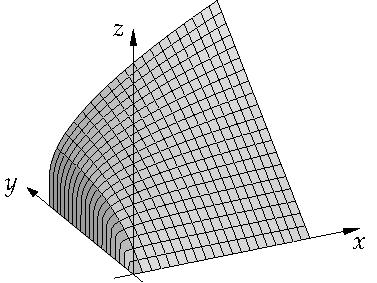
\includegraphics{figures/diffunderexample}
\caption{The graph $z= \frac{x^y-1}{\ln(x)}$ on $[0,1] \times [0,1]$.\label{fig:diffunderexample}}
\end{myfigureht}


Hence,
$g$ is a continuous function on $[0,1]$ and $g(0) = 0$.
For every $\epsilon > 0$, the $y$ derivative of the integrand, $x^y$,
is continuous on $[0,1] \times [\epsilon,1]$.  Therefore,
for $y >0$, we may differentiate under the integral sign,
\begin{equation*}
g'(y) =
\int_0^{1} \frac{\ln(x) x^y}{\ln(x)} \,dx 
=
\int_0^{1} x^y \,dx =
\frac{1}{y+1} .
\end{equation*}
We need to figure out $g(1)$ given that $g'(y) = \frac{1}{y+1}$ and $g(0) =
0$.  Elementary calculus says that $g(1) = \int_0^1 g'(y)\,dy = \ln(2)$.
Thus,
\begin{equation*}
\int_0^{1} \frac{x-1}{\ln(x)} \,dx  = \ln(2).
\end{equation*}
\end{example}

\subsection{Exercises}

\begin{exercise} \label{exercise:counterexamplediffunder}
Prove the two statements that were asserted in
\exampleref{example:counterexamplediffunder}:
\begin{enumerate}[a)]
\item
Prove $\frac{x-1}{\ln(x)}$ extends to a continuous function of
$[0,1]$.  That is, there exists a continuous function on $[0,1]$
that equals $\frac{x-1}{\ln(x)}$ on $(0,1)$.
\item
Prove $\frac{x^y-1}{\ln(x)}$ extends to a continuous function
on $[0,1] \times [0,1]$.
\end{enumerate}
\end{exercise}

\begin{exercise}
Suppose $h \colon \R \to \R$ is continuous and $g
\colon \R \to \R$ is continuously differentiable and compactly
supported.  That is, there exists some $M > 0$, such that $g(x) = 0$ whenever
$\abs{x} \geq M$.  Define
\begin{equation*}
f(x) \coloneqq \int_{-\infty}^\infty h(y)g(x-y)\,dy  .
\end{equation*}
Show that $f$ is differentiable.
\end{exercise}

\begin{exercise}
Suppose $f \colon \R \to \R$ is infinitely differentiable (all derivatives exist)
such that $f(0) = 0$.  Then show that there exists an infinitely
differentiable function $g \colon \R \to \R$ such that $f(x) = x\,g(x)$.
Show also that
if $f'(0) \not= 0$, then $g(0) \not= 0$.\\
Hint: Write
$f(x) = \int_0^x f'(s) \,ds$ and then rewrite the integral to go
from $0$ to $1$.
\end{exercise}

\begin{exercise}
Compute $\int_0^1 e^{tx} \,dx$.  Derive the formula for
$\int_0^1 x^n e^{x} \,dx$ not using integration by parts, but
by differentiation underneath the integral.
\end{exercise}

\begin{exercise}
Let $U \subset \R^n$ be an open set and suppose
$f(x,y_1,y_2,\ldots,y_n)$ is a continuous
function defined on $[0,1] \times U \subset \R^{n+1}$.
Suppose
$\frac{\partial f}{\partial y_1},
\frac{\partial f}{\partial y_2},\ldots,
\frac{\partial f}{\partial y_n}$
exist and are continuous on $[0,1] \times U$.
Then prove that $F \colon U \to \R$ defined by
\begin{equation*}
F(y_1,y_2,\ldots,y_n) \coloneqq
\int_0^1
f(x,y_1,y_2,\ldots,y_n)
\, dx
\end{equation*}
is continuously differentiable.
\end{exercise}

\begin{myfigureht}
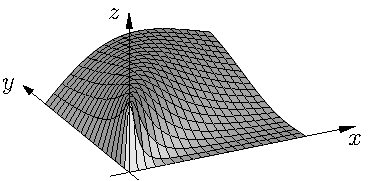
\includegraphics{figures/diffunderex916}
\caption{The graph $z= \frac{xy^3}{{(x^2+y^2)}^2}$ on
$[0,1] \times [0,1]$.\label{fig:diffunderex916}}
\end{myfigureht}

\begin{exercise}
\pagebreak[2]
Work out the following counterexample:  Let
\begin{equation*}
f(x,y) \coloneqq
\begin{cases}
\frac{xy^3}{{(x^2+y^2)}^2} & \text{if } x\not=0 \text{ or } y\not= 0, \\
0                          & \text{if } x=0 \text{ and } y=0.
\end{cases}
\end{equation*}
See \figureref{fig:diffunderex916}.
\begin{enumerate}[a)]
\item
Prove that for every fixed $y$, the function $x \mapsto f(x,y)$ is
Riemann integrable on $[0,1]$, and
\begin{equation*}
g(y) \coloneqq \int_0^1 f(x,y) \, dx = \frac{y}{2y^2+2} .
\end{equation*}
Therefore, $g'(y)$ exists and its derivative is the continuous function
\begin{equation*}
g'(y) =
\frac{d}{dy} \int_0^1 f(x,y) \, dx
=
\frac{1-y^2}{2{(y^2+1)}^2} .
\end{equation*}
\item
Prove $\frac{\partial f}{\partial y}$ exists at all $x$ and $y$ and
compute it.
\item
Show that for all $y$
\begin{equation*}
\int_0^1 \frac{\partial f}{\partial y} (x,y) \, dx
\end{equation*}
exists, but
\begin{equation*}
g'(0) \not= \int_0^1 \frac{\partial f}{\partial y} (x,0) \, dx .
\end{equation*}
\end{enumerate}
\end{exercise}

\begin{exercise}
\pagebreak[2]
Work out the following counterexample:  Let
\begin{equation*}
f(x,y) \coloneqq
\begin{cases}
x \,\sin \left(\frac{y}{x^2+y^2}\right) & \text{if } (x,y) \not= (0,0),\\
0                                       & \text{if } (x,y)=(0,0).
\end{cases}
\end{equation*}
\begin{enumerate}[a)]
\item
Prove $f$ is continuous on all of $\R^2$.
Therefore the following function is well-defined for every $y \in \R$:
\begin{equation*}
g(y) \coloneqq \int_0^1 f(x,y) \, dx .
\end{equation*}
\item
Prove $\frac{\partial f}{\partial y}$ exists for all $(x,y)$,
but is not continuous at $(0,0)$.
\item
Show that $\int_0^1 \frac{\partial f}{\partial y}(x,0) \, dx$ does not
exist even if we take improper integrals, that is,
that the limit
$\lim\limits_{h \to 0^+} \int_h^1 \frac{\partial f}{\partial y}(x,0) \, dx$
does not exist.
\end{enumerate}
Note: Feel free to use what you know about sine and cosine from calculus.
\end{exercise}

\begin{exercise} \label{exercise:strongerleibniz}
\pagebreak[3]
Strengthen the Leibniz integral rule in the following way.
Suppose $f \colon (a,b) \times (c,d) \to \R$ is a bounded continuous function,
such that $\frac{\partial f}{\partial y}$ exists for all $(x,y) \in (a,b)
\times (c,d)$ and is continuous and bounded.  Define
\begin{equation*}
g(y) \coloneqq \int_a^b f(x,y) \,dx .
\end{equation*}
Then $g \colon (c,d) \to \R$ is continuously differentiable and
\begin{equation*}
g'(y) = \int_a^b \frac{\partial f}{\partial y}(x,y) \,dx .
\end{equation*}
Hint: See also \volIref{\exerciseref*{vI-exercise:integralcontcontextra} and
\thmref*{vI-thm:dersconverge} from
volume I}{\exerciseref{exercise:integralcontcontextra} and
\thmref{thm:dersconverge}}.
\end{exercise}

%%%%%%%%%%%%%%%%%%%%%%%%%%%%%%%%%%%%%%%%%%%%%%%%%%%%%%%%%%%%%%%%%%%%%%%%%%%%%%

\sectionnewpage
\section{Path integrals}
\label{sec:pathintegral}

\sectionnotes{2--3 lectures}

\subsection{Piecewise smooth paths}

Let $\gamma \colon [a,b] \to \R^n$ be a function and write
$\gamma = (\gamma_1,\gamma_2,\ldots,\gamma_n)$. 
Suppose $\gamma$ is 
\emph{continuously differentiable},
that is,
it is differentiable and the derivative is continuous.
In other words, there exists a continuous function $\gamma^{\:\prime} \colon [a,b]
\to \R^n$ such that for every $t \in [a,b]$, we have
$\lim\limits_{h \to 0}
\frac{\snorm{\gamma(t+h)-\gamma(t) - \gamma^{\:\prime}(t) \, h}}{\sabs{h}} = 0$.
We treat
$\gamma^{\:\prime}(t)$ either as a linear operator (an $n \times 1$ matrix) or
a vector,
$\gamma^{\:\prime}(t) =
\bigl( \gamma_1^{\:\prime}(t), \gamma_2^{\:\prime}(t), \ldots,
\gamma_n^{\:\prime}(t) \bigr)$.
Equivalently, 
$\gamma_j$ is a continuously differentiable function on $[a,b]$
for every $j=1,2,\ldots,n$.
By \exerciseref{exercise:normonedim}, the operator norm of
the operator $\gamma^{\:\prime}(t)$ is equal to
the euclidean norm of the corresponding vector, so there is no
confusion when writing $\snorm{\gamma^{\:\prime}(t)}$.

\begin{defn}
A continuously differentiable function $\gamma \colon [a,b] \to \R^n$ is
called a \emph{\myindex{smooth path}}
or a
\emph{\myindex{continuously differentiable path}}\footnote{The
word \myquote{smooth} can sometimes mean
\myquote{infinitely differentiable} in the literature.}
if
$\gamma$ is continuously differentiable and
$\gamma^{\:\prime}(t) \not= 0$ for all $t \in [a,b]$.

The function $\gamma \colon [a,b] \to \R^n$ is called a
\emph{\myindex{piecewise smooth path}} or a
\emph{\myindex{piecewise continuously differentiable path}}
if there exist finitely many points
$t_0 = a < t_1 < t_2 < \cdots < t_k = b$ such that
the restriction $\gamma|_{[t_{j-1},t_j]}$ is smooth path for every
$j=1,2,\ldots,k$.

A path $\gamma$ is 
a \emph{\myindex{closed path}} if $\gamma(a) = \gamma(b)$, that is
if the path starts and ends in the same point.
A path $\gamma$ is a \emph{\myindex{simple path}} if 
either 1) $\gamma$ is a one-to-one function, or 2)
$\gamma|_{[a,b)}$ is one-to-one and $\gamma(a)=\gamma(b)$ ($\gamma$ is a
simple closed path).
\end{defn}


\begin{example} \label{mv:example:unitsquarepath}
Let $\gamma \colon [0,4] \to \R^2$ be defined by
\begin{equation*}
\gamma(t) \coloneqq
\begin{cases}
(t,0)   & \text{if } t \in [0,1],\\
(1,t-1) & \text{if } t \in (1,2],\\
(3-t,1) & \text{if } t \in (2,3],\\
(0,4-t) & \text{if } t \in (3,4].
\end{cases}
\end{equation*}
\begin{myfigureht}
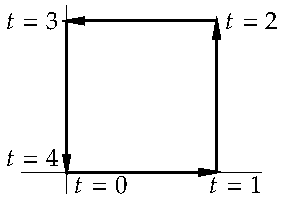
\includegraphics{figures/squarepath}
\caption{The path $\gamma$ traversing the unit square.\label{fig:squarepath}}
\end{myfigureht}

The path $\gamma$ is the unit square traversed
counterclockwise.  See \figureref{fig:squarepath}.  It is
a piecewise smooth path.  For example,
$\gamma|_{[1,2]}(t) = (1,t-1)$ and so
$(\gamma|_{[1,2]})'(t) = (0,1) \not= 0$.  Similarly for the other 3 sides.
Notice
that
$(\gamma|_{[1,2]})'(1) = (0,1)$,
$(\gamma|_{[0,1]})'(1) = (1,0)$, but
$\gamma^{\:\prime}(1)$ does not exist.  At the corners $\gamma$ is 
not differentiable.
The path $\gamma$ is a simple closed path, as $\gamma|_{[0,4)}$ is
one-to-one and $\gamma(0)=\gamma(4)$.
\end{example}

The definition of a piecewise smooth path as we have given it implies
continuity (exercise).  For general functions, many authors also
allow finitely many discontinuities, when they use the term \emph{piecewise
smooth}, and so one may say that we defined a piecewise smooth path
to be a \emph{\myindex{continuous piecewise smooth}} function.
While one may get by with smooth paths, for computations, the simplest
paths to write down are often piecewise smooth.

Generally, we are interested in the direct image $\gamma\bigl([a,b]\bigr)$,
rather than the specific parametrization, although that is also
important to some degree.  When we informally talk about a path or a curve,
we often mean the set $\gamma\bigl([a,b]\bigr)$, depending
on context.


\begin{example}
The condition $\gamma^{\:\prime}(t) \not= 0$ means that the image
$\gamma\bigl([a,b]\bigr)$
has no \myquote{corners} where $\gamma$ is smooth.
Consider 
\begin{equation*}
\gamma(t) \coloneqq
\begin{cases}
(t^2,0) & \text{if } t < 0,\\
(0,t^2) & \text{if } t \geq 0.
\end{cases}
\end{equation*}
See \figureref{fig:cornersmoothpath}.
It is left for the reader to check that $\gamma$ is continuously
differentiable, yet the image $\gamma(\R) = \bigl\{ (x,y) \in \R^2 : (x,y) =
(s,0) \text{ or } (x,y) = (0,s) \text{ for some } s \geq 0 \bigr\}$ has a
\myquote{corner} at the origin.  And that is because $\gamma^{\:\prime}(0) = (0,0)$.
More complicated examples with, say, infinitely many corners exist,
see the exercises.
\begin{myfigureht}
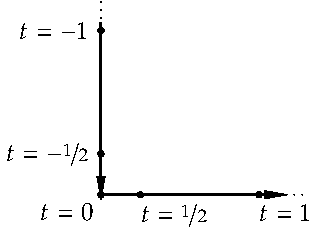
\includegraphics{figures/cornersmoothpath}
\caption{Smooth path with zero derivative with a corner.  Several values of
$t$ are marked with dots.\label{fig:cornersmoothpath}}
\end{myfigureht}
\end{example}

The condition $\gamma^{\:\prime}(t) \not= 0$ even at the endpoints guarantees
not only no corners, but also that the path ends nicely, that is, it can
extend a little bit past the endpoints.  Again, see the exercises.

\begin{example}
A graph of a continuously differentiable function $f \colon [a,b] \to \R$ is a smooth path.
Define $\gamma \colon [a,b] \to \R^2$ by
\begin{equation*}
\gamma(t) \coloneqq \bigl(t,f(t)\bigr) .
\end{equation*}
Then $\gamma^{\:\prime}(t) = \bigl( 1 , f'(t) \bigr)$, which is never zero,
and $\gamma\bigl([a,b]\bigr)$ is the graph of $f$.

There are other ways of parametrizing the path.  That is, there are
different paths with the same image.
The function $t \mapsto (1-t)a+tb$, takes the interval $[0,1]$ to $[a,b]$.
Define
$\alpha \colon [0,1] \to \R^2$ by
\begin{equation*}
\alpha(t) \coloneqq \bigl((1-t)a+tb,f((1-t)a+tb)\bigr) .
\end{equation*}
Then
$\alpha'(t) = \bigl( b-a ,~ (b-a)f'((1-t)a+tb) \bigr)$, which is never zero.
As sets, $\alpha\bigl([0,1]\bigr) = \gamma\bigl([a,b]\bigr)
= \bigl\{ (x,y) \in \R^2 : x \in [a,b] \text{ and } f(x) = y \bigr\}$,
which is just the graph of $f$.
\end{example}

The last example leads us to a definition.

\begin{defn}
Let $\gamma \colon [a,b] \to \R^n$ be a smooth path and
$h \colon [c,d] \to [a,b]$ a continuously differentiable bijective function
such that $h'(t) \not= 0$ for all $t \in [c,d]$.  Then
the composition
$\gamma \circ h$ is called a
\emph{\myindex{smooth reparametrization}}\index{reparametrization}
of $\gamma$.

Let $\gamma$ be a piecewise smooth path, and
$h$ a piecewise smooth bijective function with
nonzero one-sided limits of $h'$.
The composition
$\gamma \circ h$ is called a
\emph{\myindex{piecewise smooth reparametrization}} of $\gamma$.

If $h$ is strictly increasing, then $h$ is 
said to \emph{\myindex{preserve orientation}}.  If $h$ does not preserve
orientation, then $h$ is said to \emph{\myindex{reverse orientation}}.
\end{defn}

A reparametrization is another path for the same set.  That is,
$(\gamma \circ h)\bigl([c,d]\bigr) =
\gamma \bigl([a,b]\bigr)$.

The conditions on the piecewise smooth $h$ mean that
there is some partition $t_0 = c < t_1 < t_2 < \cdots < t_k = d$,
such that $h|_{[t_{j-1},t_j]}$ is continuously differentiable
and $(h|_{[t_{j-1},t_j]})'(t) \not= 0$ for all $t \in [t_{j-1},t_j]$.
Since $h$ is bijective, it is either strictly increasing or
strictly decreasing.  So either $(h|_{[t_{j-1},t_j]})'(t) > 0$
for all $t$ or $(h|_{[t_{j-1},t_j]})'(t) < 0$ for all $t$.

\begin{prop} \label{prop:reparamapiecewisesmooth}
If $\gamma \colon [a,b] \to \R^n$ is a piecewise smooth path,
and $\gamma \circ h \colon [c,d] \to \R^n$ is
a piecewise smooth reparametrization, then $\gamma \circ h$
is a piecewise smooth path.
\end{prop}

\begin{proof}
Assume that $h$ preserves orientation, that is, $h$ is strictly
increasing.
If $h \colon [c,d] \to [a,b]$ gives a piecewise smooth reparametrization,
then for some partition
$r_0 = c < r_1 < r_2 < \cdots < r_\ell = d$, the restriction
$h|_{[r_{j-1},r_j]}$ is continuously differentiable with a positive
derivative.

Let $t_0 = a < t_1 < t_2 < \cdots < t_k = b$ be the partition from the
definition of piecewise smooth for $\gamma$ together with the 
points $\{ h(r_0), h(r_1), h(r_2), \ldots, h(r_\ell) \}$.
Let $s_j \coloneqq h^{-1}(t_j)$.  Then
$s_0 = c < s_1 < s_2 < \cdots < s_k = d$
is a partition that includes (is a refinement of) the
$\{ r_0,r_1,\ldots,r_\ell \}$.
If $\tau \in [s_{j-1},s_j]$, then $h(\tau) \in [t_{j-1},t_j]$
since $h(s_{j-1}) = t_{j-1}$,
$h(s_{j}) = t_j$, and
$h$ is strictly increasing.
Also $h|_{[s_{j-1},s_j]}$ is continuously differentiable, and
$\gamma|_{[t_{j-1},t_j]}$ is also continuously differentiable.
Then
\begin{equation*}
(\gamma \circ h)|_{[s_{j-1},s_{j}]} (\tau)
=
\gamma|_{[t_{j-1},t_{j}]} \bigl( h|_{[s_{j-1},s_j]}(\tau) \bigr) .
\end{equation*}
The function 
$(\gamma \circ h)|_{[s_{j-1},s_{j}]}$ is therefore continuously
differentiable and
by the chain rule
\begin{equation*}
\bigl( (\gamma \circ h)|_{[s_{j-1},s_{j}]} \bigr) ' (\tau)
=
\bigl( \gamma|_{[t_{j-1},t_{j}]} \bigr)' \bigl( h(\tau) \bigr)
(h|_{[s_{j-1},s_j]})'(\tau) \not= 0 .
\end{equation*}
Consequently, $\gamma \circ h$ is a piecewise smooth path.
Orientation reversing $h$ is left as an exercise.
\end{proof}

If two paths are simple and their images are the same, it is
left as an exercise that there exists a reparametrization.
Here is where our assumption that $\gamma'$ is never zero is important.

\subsection{Path integral of a one-form}

\begin{defn}
Let $(x_1,x_2,\ldots,x_n) \in \R^n$ be our coordinates.
Given $n$ real-valued continuous functions
$\omega_1,\omega_2,\ldots,\omega_n$ defined on a set $S \subset \R^n$,
we define a \emph{\myindex{one-form}}\index{differential one-form}
to be an object of the form
\glsadd{not:oneform}
\begin{equation*}
\omega = \omega_1 \,dx_1 + \omega_2 \,dx_2 + \cdots + \omega_n \,dx_n .
\end{equation*}
We could represent $\omega$ as a continuous function from $S$ to $\R^n$,
although it is better to think of it as a different object.
\end{defn}

\begin{example}
\begin{equation*}
\omega(x,y) \coloneqq \frac{-y}{x^2+y^2} \,dx + \frac{x}{x^2+y^2} \,dy
\end{equation*}
is a one-form defined on $\R^2 \setminus \{ (0,0) \}$.
\end{example}

\begin{defn}
Let $\gamma \colon [a,b] \to \R^n$ be a smooth path
and let
\begin{equation*}
\omega = \omega_1 \,dx_1 + \omega_2 \,dx_2 + \cdots + \omega_n \,dx_n ,
\end{equation*}
be a one-form defined on the direct image $\gamma\bigl([a,b]\bigr)$.
Write $\gamma = (\gamma_1,\gamma_2,\ldots,\gamma_n)$.
Define:
\begin{equation*}
\begin{split}
\int_{\gamma} \omega
& \coloneqq
\int_a^b 
\Bigl(
\omega_1\bigl(\gamma(t)\bigr) \gamma_1^{\:\prime}(t) +
\omega_2\bigl(\gamma(t)\bigr) \gamma_2^{\:\prime}(t) + \cdots +
\omega_n\bigl(\gamma(t)\bigr) \gamma_n^{\:\prime}(t) \Bigr) dt
\\
&\phantom{:}=
\int_a^b 
\left(
\sum_{j=1}^n
\omega_j\bigl(\gamma(t)\bigr) \gamma_j^{\:\prime}(t) \right) dt .
\end{split}
\end{equation*}
To remember the definition note that $x_j$ is $\gamma_j(t)$, so
$dx_j$ becomes  $\gamma_j^{\:\prime}(t) \, dt$.

If $\gamma$ is piecewise smooth, take the corresponding partition
$t_0 = a < t_1 < t_2 < \ldots < t_k = b$, and assume the partition is
minimal
%\footnote{This restriction is not strictly necessary, but it 
%makes the integral immediately well-defined.}
in the sense that $\gamma$ is not differentiable
at $t_1,t_2,\ldots,t_{k-1}$.  As each $\gamma|_{[t_{j-1},t_j]}$ is
a smooth path, define
\begin{equation*}
\int_{\gamma} \omega
\coloneqq
\int_{\gamma|_{[t_0,t_1]}} \omega
\,
+
\,
\int_{\gamma|_{[t_1,t_2]}} \omega
\,
+ \, \cdots \, + \,
\int_{\gamma|_{[t_{k-1},t_k]}} \omega .
\end{equation*}
\end{defn}

The notation makes sense from the formula you remember from calculus,
let us state it somewhat informally:
If $x_j(t) = \gamma_j(t)$, then $dx_j = \gamma_j^{\:\prime}(t) \, dt$.

Paths can be cut up or concatenated.  The proof is a direct application
of the additivity of the Riemann integral, and is left as an exercise.
The proposition justifies why we defined the integral over a piecewise
smooth path in the way we did, and it justifies that we may as well
have taken any partition not just the minimal one in the definition.

\begin{prop} \label{mv:prop:pathconcat}
Let $\gamma \colon [a,c] \to \R^n$ be a piecewise smooth path,
and $b \in (a,c)$.
Define the piecewise smooth paths
$\alpha \coloneqq \gamma|_{[a,b]}$ and
$\beta \coloneqq \gamma|_{[b,c]}$.
Let $\omega$ be a one-form defined on
$\gamma\bigl([a,c]\bigr)$.  Then
\begin{equation*}
\int_{\gamma} \omega =
\int_{\alpha} \omega +
\int_{\beta} \omega .
\end{equation*}
\end{prop}


\begin{example} \label{example:mv:irrotoneformint}
Let the one-form $\omega$ and the path $\gamma \colon [0,2\pi] \to \R^2$ be defined by
\begin{equation*}
\omega(x,y) \coloneqq \frac{-y}{x^2+y^2} \,dx + \frac{x}{x^2+y^2} \,dy,
\qquad
\gamma(t) \coloneqq \bigl(\cos(t),\sin(t)\bigr) .
\end{equation*}
Then
\begin{equation*}
\begin{split}
\int_{\gamma} \omega
& =
\int_0^{2\pi}
\Biggl(
\frac{-\sin(t)}{{\bigl(\cos(t)\bigr)}^2+{\bigl(\sin(t)\bigr)}^2}
\bigl(-\sin(t)\bigr)
+
\frac{\cos(t)}{{\bigl(\cos(t)\bigr)}^2+{\bigl(\sin(t)\bigr)}^2}
\bigl(\cos(t)\bigr)
\Biggr) \, dt
\\
& =
\int_0^{2\pi}
1 \, dt
= 2\pi .
\end{split}
\end{equation*}
Next, let us parametrize the same curve as
$\alpha \colon [0,1] \to \R^2$ defined by $\alpha(t) \coloneqq \bigl(\cos(2\pi
t),\sin(2 \pi t)\bigr)$, that is $\alpha$ is a smooth reparametrization of
$\gamma$.  Then
\begin{equation*}
\begin{split}
\int_{\alpha} \omega
& =
\int_0^{1}
\Biggl(
\frac{-\sin(2\pi t)}{{\bigl(\cos(2\pi t)\bigr)}^2+{\bigl(\sin(2\pi t)\bigr)}^2}
\bigl(-2\pi \sin(2\pi t)\bigr)
\\
& \phantom{=\int_0^1\Biggl(~}
+
\frac{\cos(2 \pi t)}{{\bigl(\cos(2 \pi t)\bigr)}^2+{\bigl(\sin(2 \pi t)\bigr)}^2}
\bigl(2 \pi \cos(2 \pi t)\bigr)
\Biggr) \, dt
\\
& =
\int_0^{1}
2\pi \, dt
= 2\pi .
\end{split}
\end{equation*}
Now let us reparametrize with $\beta \colon [0,2\pi] \to \R^2$
as $\beta(t) \coloneqq \bigl(\cos(-t),\sin(-t)\bigr)$.  Then
\begin{equation*}
\begin{split}
\int_{\beta} \omega
& =
\int_0^{2\pi}
\Biggl(
\frac{-\sin(-t)}{{\bigl(\cos(-t)\bigr)}^2+{\bigl(\sin(-t)\bigr)}^2}
\bigl(\sin(-t)\bigr)
+
\frac{\cos(-t)}{{\bigl(\cos(-t)\bigr)}^2+{\bigl(\sin(-t)\bigr)}^2}
\bigl(-\cos(-t)\bigr)
\Biggr) \, dt
\\
& =
\int_0^{2\pi}
(-1) \, dt
= -2\pi .
\end{split}
\end{equation*}
The path $\alpha$ is an orientation preserving reparametrization of
$\gamma$, and the integrals are the same.  The path $\beta$
is an orientation reversing reparametrization of $\gamma$ and the integral is
minus the original.  See \figureref{fig:circlepathrepar}.
\begin{myfigureht}
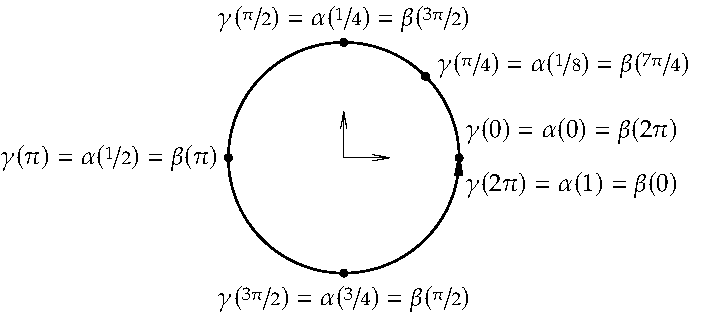
\includegraphics{figures/circlepathrepar}
\caption{A circular path reparametrized in two different ways. The arrow
indicates the orientation of $\gamma$ and $\alpha$. The path $\beta$ traverses
the circle in the
opposite direction.\label{fig:circlepathrepar}}
\end{myfigureht}
\end{example}

The previous example is not a fluke.
The path integral does not depend on the parametrization of
the curve, the only thing that matters is the direction in which the curve
is traversed.

\begin{prop} \label{mv:prop:pathintrepararam}
Let $\gamma \colon [a,b] \to \R^n$ be a piecewise smooth path and
$\gamma \circ h \colon [c,d] \to \R^n$ a piecewise smooth reparametrization.
Suppose $\omega$ is a one-form defined on the set $\gamma\bigl([a,b]\bigr)$.  Then
\begin{equation*}
\int_{\gamma \circ h} \omega =
\begin{cases}
\int_{\gamma} \omega  & \text{if } h \text{ preserves orientation,}\\
-\int_{\gamma} \omega & \text{if } h \text{ reverses orientation.}
\end{cases}
\end{equation*}
\end{prop}

\begin{proof}
Assume first that $\gamma$ and $h$ are both smooth.
Write $\omega = \omega_1 \, dx_1 + \omega_2 \, dx_2 + \cdots +
\omega_n \, dx_n$.
Suppose that $h$ is orientation preserving.  Use
the change of variables formula for the Riemann integral:
\begin{equation*}
\begin{split}
\int_{\gamma} \omega
& =
\int_a^b 
\left(
\sum_{j=1}^n
\omega_j\bigl(\gamma(t)\bigr) \gamma_j^{\:\prime}(t)
\right) dt
\\
& =
\int_c^d 
\left(
\sum_{j=1}^n
\omega_j\Bigl(\gamma\bigl(h(\tau)\bigr)\Bigr) \gamma_j^{\:\prime}\bigl(h(\tau)\bigr)
\right) h'(\tau) \, d\tau
\\
& =
\int_c^d 
\left(
\sum_{j=1}^n
\omega_j\Bigl(\gamma\bigl(h(\tau)\bigr)\Bigr) (\gamma_j \circ h)'(\tau)
\right) d\tau
=
\int_{\gamma \circ h} \omega .
\end{split}
\end{equation*}
If $h$ is orientation reversing, it swaps the order of the limits on the
integral and introduces a minus sign.
The details, along with finishing the proof for piecewise smooth
paths, is left as \exerciseref{mv:exercise:pathpiece}.
\end{proof}

Due to this proposition (and the exercises), if $\Gamma
\subset \R^n$ is the image of a simple piecewise smooth path
$\gamma\bigl([a,b]\bigr)$, then as long as we somehow indicate the orientation, that
is, the direction in which we traverse the curve, we can write
\begin{equation*}
\int_{\Gamma} \omega ,
\end{equation*}
without mentioning the specific $\gamma$.
Furthermore, for a simple closed path, it does not even matter where we
start the parametrization.  See the exercises.

Recall that \emph{simple} means that $\gamma$
is one-to-one except perhaps at the endpoints, in particular
it is one-to-one when restricted to $[a,b)$.
We may relax the condition that the path is simple a little bit.
For example, it is enough to suppose that
$\gamma \colon [a,b] \to \R^n$ is one-to-one except at finitely many points.
%That is, there is a finite set $S \subset [a,b]$
%and $\gamma|_{[a,b]\setminus S}$ is one-to-one.
See \exerciseref{mv:exercise:curveintegral}.  But we cannot remove
the condition completely as is
illustrated by the following example.

\begin{example}
Suppose $\gamma \colon [0,2\pi] \to \R^2$ is given by $\gamma(t) \coloneqq
\bigl(\cos(t),\sin(t)\bigr)$, and
$\beta \colon [0,2\pi] \to \R^2$ by $\beta(t) \coloneqq
\bigl(\cos(2t),\sin(2t)\bigr)$.  Notice that
$\gamma\bigl([0,2\pi]\bigr) = \beta\bigl([0,2\pi]\bigr)$; we travel
around the same curve, the unit circle.  But $\gamma$ goes around the unit
circle once in the counter clockwise direction, and $\beta$ goes around the
unit circle twice (in the same direction). 
See \figureref{fig:circlepathrepar2}.
\begin{myfigureht}
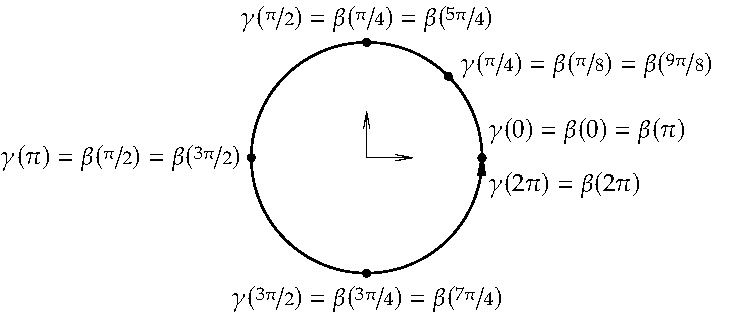
\includegraphics{figures/circlepathrepar2}
\caption{Circular path traversed once by
$\gamma \colon [0,2\pi] \to \R^2$
and twice by
$\beta \colon [0,2\pi] \to \R^2$.\label{fig:circlepathrepar2}}
\end{myfigureht}

Compute
\begin{align*}
& \int_{\gamma} -y\, dx + x\,dy
=
\int_0^{2\pi}
\Bigl( \bigl(-\sin(t) \bigr) \bigl(-\sin(t) \bigr) + \cos(t) \cos(t) \Bigr) dt
=
2 \pi,\\
& \int_{\beta} -y\, dx + x\,dy
=
\int_0^{2\pi}
\Bigl( \bigl(-\sin(2t) \bigr) \bigl(-2\sin(2t) \bigr) + \cos(t)
\bigl(2\cos(t)\bigr) \Bigr) dt
=
4 \pi.
\end{align*}
\end{example}

It is sometimes convenient to define a path integral over $\gamma \colon
[a,b] \to \R^n$ that is not a path.
Define
\glsadd{not:pathintegralomega}
\begin{equation*}
\int_{\gamma} \omega \coloneqq \int_a^b
\left(
\sum_{j=1}^n
\omega_j\bigl(\gamma(t)\bigr) \gamma_j^{\:\prime}(t)
\right) dt 
\end{equation*}
for every continuously differentiable $\gamma$.  A 
case that comes up naturally is when $\gamma$ is constant.  Then
$\gamma^{\:\prime}(t) = 0$ for all $t$, and $\gamma\bigl([a,b]\bigr)$ is a single
point, which we regard as a \myquote{curve} of length zero.  Then,
$\int_{\gamma} \omega = 0$ for every $\omega$.

\subsection{Path integral of a function}

Next, we integrate a function against the so-called
\emph{\myindex{arc-length measure}} $ds$.  The geometric picture we have in mind
is the area under the graph of the function over a path.
Imagine a fence erected over $\gamma$ with height given by the function
and the integral is the area of the fence.
See \figureref{fig:fenceintegral}.
\begin{myfigureht}
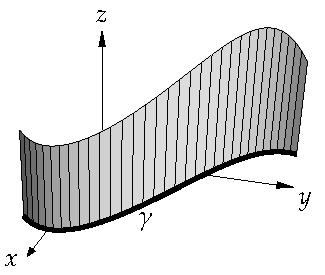
\includegraphics{figures/fenceintegral}
\caption{A path $\gamma \colon [a,b] \to \R^2$ in the $xy$-plane (bold curve), and a function
$z=f(x,y)$ graphed above it in the $z$ direction.  The integral is the
shaded area depicted.\label{fig:fenceintegral}}
\end{myfigureht}

\begin{defn}
Suppose $\gamma \colon [a,b] \to \R^n$ is a smooth path, and $f$ is a
continuous function defined on the image $\gamma\bigl([a,b]\bigr)$.  Then
define
\glsadd{not:lineintegralf}
\begin{equation*}
\int_{\gamma} f \,ds \coloneqq
\int_a^b f\bigl( \gamma(t) \bigr) \snorm{\gamma^{\:\prime}(t)} \, dt .
\end{equation*}
To emphasize the variables we may use
\begin{equation*}
\int_{\gamma} f(x) \,ds(x) \coloneqq \int_{\gamma} f \,ds .
\end{equation*}

The definition for a piecewise smooth path is similar as before and is left
to the reader.
\end{defn}

The path integral of a function is also independent of the parametrization,
and in this case, the orientation does not matter.

\begin{prop} \label{mv:prop:lineintrepararam}
Let $\gamma \colon [a,b] \to \R^n$ be a piecewise smooth path and
$\gamma \circ h \colon [c,d] \to \R^n$ a piecewise smooth reparametrization.
Suppose $f$ is a continuous function defined on the set
$\gamma\bigl([a,b]\bigr)$.  Then
\begin{equation*}
\int_{\gamma \circ h} f\, ds = \int_{\gamma} f\, ds .
\end{equation*}
\end{prop}

\begin{proof}
Suppose $h$ is orientation preserving and that $\gamma$ and $h$
are both smooth.  Then 
\begin{equation*}
\begin{split}
\int_{\gamma} f \, ds
& =
\int_a^b 
f\bigl(\gamma(t)\bigr) \snorm{\gamma^{\:\prime}(t)} \, dt
\\
& =
\int_c^d 
f\Bigl(\gamma\bigl(h(\tau)\bigr)\Bigr)
\snorm{\gamma^{\:\prime}\bigl(h(\tau)\bigr)} h'(\tau) \, d\tau
\\
& =
\int_c^d 
f\Bigl(\gamma\bigl(h(\tau)\bigr)\Bigr)
\snorm{\gamma^{\:\prime}\bigl(h(\tau)\bigr) h'(\tau)} \, d\tau
\\
& =
\int_c^d 
f\bigl((\gamma \circ h)(\tau)\bigr) \snorm{(\gamma \circ h)'(\tau)} \, d\tau
\\
& = 
\int_{\gamma \circ h} f \, ds .
\end{split}
\end{equation*}
If $h$ is orientation reversing it swaps the order of the limits on the
integral, but you also have to introduce a minus sign in order
to take $h'$ inside the norm.
The details, along with finishing the proof for piecewise smooth
paths is left to the reader as \exerciseref{mv:exercise:linepiece}.
\end{proof}

As before,
due to this proposition (and the exercises),
if $\gamma$ is simple, it does not matter which
parametrization we use.  Therefore, if $\Gamma = \gamma\bigl( [a,b] \bigr)$, we can
simply write
\begin{equation*}
\int_\Gamma f\, ds .
\end{equation*}
In this case we do not need to worry about orientation, either way we
get the same integral.

\begin{example}
Let $f(x,y) \coloneqq x$.  Let $C \subset \R^2$ be half of the unit circle for $x
\geq 0$.  We wish to compute
\begin{equation*}
\int_C f \, ds .
\end{equation*}
Parametrize the curve $C$ via $\gamma \colon
[\nicefrac{-\pi}{2},\nicefrac{\pi}{2}] \to \R^2$ defined as
$\gamma(t) \coloneqq \bigl(\cos(t),\sin(t)\bigr)$.
Then $\gamma^{\:\prime}(t) = \bigl(-\sin(t),\cos(t)\bigr)$, and
\begin{equation*}
\int_C f \, ds =
\int_\gamma f \, ds
=
\int_{-\pi/2}^{\pi/2} \cos(t) \sqrt{ {\bigl(-\sin(t)\bigr)}^2 +  
{\bigl(\cos(t)\bigr)}^2 } \, dt
=
\int_{-\pi/2}^{\pi/2} \cos(t) \, dt = 2.
\end{equation*}
\end{example}

\begin{defn}
Suppose $\Gamma \subset \R^n$ is parametrized by a simple
piecewise smooth path $\gamma \colon [a,b] \to \R^n$, that is
$\gamma\bigl( [a,b] \bigr) = \Gamma$.  We define the
\emph{\myindex{length}}\index{length of a curve} by
\begin{equation*}
\ell(\Gamma) \coloneqq \int_{\Gamma} ds = \int_{\gamma} ds .
\end{equation*}
\end{defn}

If $\gamma$ is smooth,
\begin{equation*}
\ell(\Gamma) = 
\int_a^b
\snorm{\gamma^{\:\prime}(t)}\, dt .
\end{equation*}
This may be a good time to mention that it is common to write
$\int_a^b
\snorm{\gamma^{\:\prime}(t)}\, dt$ even if the path is only piecewise smooth.
That is because $\snorm{\gamma^{\:\prime}(t)}$ is defined and continuous
at all but finitely many points and is bounded, and so the integral exists.

\begin{example}
Let $x,y \in \R^n$ be two points and write $[x,y]$ as the straight line
segment between the two points $x$ and $y$.  Parametrize
$[x,y]$ by $\gamma(t) \coloneqq (1-t)x + ty$ for $t$ running between $0$ and $1$.
See \figureref{fig:straightpath}.
Then $\gamma^{\:\prime}(t) = y-x$, and therefore
\begin{equation*}
\ell\bigl([x,y]\bigr)
=
\int_{[x,y]} ds
=
\int_0^1 \snorm{y-x} \, dt
=
\snorm{y-x} .
\end{equation*}
The length of $[x,y]$ is the standard euclidean distance between $x$ and $y$,
justifying the name.
\begin{myfigureht}
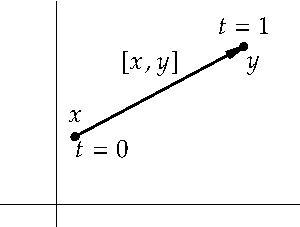
\includegraphics{figures/straightpath}
\caption{Straight path between $x$ and $y$ parametrized
by $(1-t)x + ty$.\label{fig:straightpath}}
\end{myfigureht}
\end{example}

A simple piecewise smooth path $\gamma \colon [0,r] \to \R^n$ is
said to be an \emph{\myindex{arc-length parametrization}} if
for all $t \in [0,r]$, we have
\begin{equation*}
\ell\bigl( \gamma\bigl([0,t]\bigr) \bigr) = t .
\end{equation*}
If $\gamma$ is smooth, then
\begin{equation*}
\int_0^t d\tau =
t = \ell\bigl( \gamma\bigl([0,t]\bigr) \bigr) =
\int_0^t
\snorm{\gamma^{\:\prime}(\tau)}
\, d\tau
\end{equation*}
for all $t$,
which means that $\snorm{\gamma^{\:\prime}(t)} = 1$ for all $t$.
Similarly for piecewise smooth $\gamma$, we get
$\snorm{\gamma^{\:\prime}(t)} = 1$ for all $t$ where the derivative exists.
So you can think of such a parametrization as moving around your curve at speed
1.  If $\gamma \colon [0,r] \to \R^n$ is an arclength parametrization, it is
common to use $s$ as the variable as $\int_\gamma f \,ds
= \int_0^r f\bigl(\gamma(s)\bigr) \,ds$.

\subsection{Exercises}

\begin{exercise}
Show that if $\varphi \colon [a,b] \to \R^n$ is a piecewise smooth path as we
defined it, then $\varphi$ is a continuous function.
\end{exercise}

\begin{exercise}
Finish the proof of \propref{prop:reparamapiecewisesmooth} for orientation
reversing reparametrizations.
\end{exercise}

\begin{exercise}
Prove \propref{mv:prop:pathconcat}.
\end{exercise}

\begin{exercise} \label{mv:exercise:pathpiece}
Finish the proof of \propref{mv:prop:pathintrepararam}
for
\begin{enumerate}[a)]
\item
orientation reversing reparametrizations, and
\item
piecewise smooth paths
and reparametrizations.
\end{enumerate}
\end{exercise}

\begin{exercise} \label{mv:exercise:linepiece}
Finish the proof of \propref{mv:prop:lineintrepararam}
for
\begin{enumerate}[a)]
\item
orientation reversing reparametrizations, and
\item
piecewise smooth paths
and reparametrizations.
\end{enumerate}
\end{exercise}

\begin{exercise}
Suppose $\gamma \colon [a,b] \to \R^n$ is a piecewise smooth path, and $f$ is a
continuous function defined on the image $\gamma\bigl([a,b]\bigr)$.
Provide a definition of $\int_{\gamma} f \,ds$.
\end{exercise}

\begin{exercise}
Directly using the definitions compute:
\begin{enumerate}[a)]
\item
The arc-length of the unit square from
\exampleref{mv:example:unitsquarepath} using the given parametrization.
\item
The arc-length of the unit circle using the parametrization
$\gamma \colon [0,1] \to \R^2$, $\gamma(t) \coloneqq \bigl(\cos(2\pi t),\sin(2\pi t)\bigr)$.
\item
The arc-length of the unit circle using the parametrization
$\beta \colon [0,2\pi] \to \R^2$, $\beta(t) \coloneqq \bigl(\cos(t),\sin(t)\bigr)$.
\end{enumerate}
Note: Feel free to use what you know about sine and cosine from calculus.
\end{exercise}

\begin{exercise}
Suppose $\gamma \colon [0,1] \to \R^n$ is a smooth path, and
$\omega$ is a one-form defined on the image $\gamma\bigl([a,b]\bigr)$.
For $r \in [0,1]$, let $\gamma_r \colon [0,r] \to \R^n$ be defined
as simply the restriction of $\gamma$ to $[0,r]$.  Show that the
function $h(r) \coloneqq \int_{\gamma_r} \omega$ is a continuously
differentiable function on $[0,1]$.
\end{exercise}

\begin{exercise}
Suppose $\gamma \colon [a,b] \to \R^n$ is a smooth path.
Show that there exists an $\epsilon > 0$ and a smooth function
$\widetilde{\gamma} \colon (a-\epsilon,b+\epsilon) \to \R^n$
with $\widetilde{\gamma}(t) = \gamma(t)$ for all $t \in [a,b]$
and $\widetilde{\gamma}^{\:\prime}(t) \not= 0$ for all $t \in 
(a-\epsilon,b+\epsilon)$.  That is, prove that a smooth path extends
some small distance past the end points.
\end{exercise}

\begin{exercise} 
Suppose $\alpha \colon [a,b] \to \R^n$ and
$\beta \colon [c,d] \to \R^n$ are piecewise smooth paths such that
$\Gamma \coloneqq \alpha\bigl([a,b]\bigr) = \beta\bigl([c,d]\bigr)$.
Show that there exist finitely many points
$\{ p_1,p_2,\ldots,p_k\} \in \Gamma$, such that
the sets
$\alpha^{-1}\bigl( \{ p_1,p_2,\ldots,p_k\} \bigr)$
and
$\beta^{-1}\bigl( \{ p_1,p_2,\ldots,p_k\} \bigr)$
are partitions of $[a,b]$ and $[c,d]$ such that on every subinterval
the paths are smooth (that is, they are partitions as in the definition
of piecewise smooth path).
\end{exercise}

\begin{exercise}
\pagebreak[3]
\leavevmode
\begin{enumerate}[a)]
\item
Suppose $\gamma \colon [a,b] \to \R^n$ and $\alpha \colon [c,d] \to \R^n$
are two smooth paths that are one-to-one and
$\gamma\bigl([a,b]\bigr) = \alpha\bigl([c,d]\bigr)$.  Then
there exists a smooth reparametrization $h \colon [a,b] \to [c,d]$
such that $\gamma = \alpha \circ h$.\\
Hint 1: It is not hard to show $h$ exists.
The trick is to prove it is continuously differentiable
with a nonzero derivative.  Apply the implicit function
theorem though it may at first seem the dimensions are wrong.\\
Hint 2: Worry about derivative of $h$ in $(a,b)$ first.
\item
Prove the same thing as part a, but now for simple closed paths with the
further assumption that $\gamma(a) = \gamma(b) = \alpha(c) = \alpha(d)$.
\item
Prove parts a) and b) but for piecewise smooth paths, obtaining
piecewise smooth reparametrizations.\\
Hint: The trick is to find two
partitions such that when restricted to a subinterval of the partition
both paths have the same image and are smooth, see the exercise above.
\end{enumerate}
\end{exercise}

\begin{exercise} 
\pagebreak[1]
Suppose $\alpha \colon [a,b] \to \R^n$ and
$\beta \colon [b,c] \to \R^n$ are piecewise smooth paths with
$\alpha(b)=\beta(b)$.  Let $\gamma \colon [a,c] \to \R^n$ be defined by
\begin{equation*}
\gamma(t) \coloneqq
\begin{cases}
\alpha(t) & \text{if } t \in [a,b], \\
\beta(t)  & \text{if } t \in (b,c].
\end{cases}
\end{equation*}
Show that $\gamma$ is a piecewise smooth path, and that if $\omega$ is a
one-form defined on the curve given by $\gamma$, then
\begin{equation*}
\int_{\gamma} \omega =
\int_{\alpha} \omega +
\int_{\beta} \omega .
\end{equation*}
\end{exercise}

\begin{exercise} \label{mv:exercise:closedcurveintegral}
\pagebreak[1]
Suppose $\gamma \colon [a,b] \to \R^n$ and
$\beta \colon [c,d] \to \R^n$ are two simple closed piecewise smooth paths.
That is, $\gamma(a)=\gamma(b)$ and $\beta(c) = \beta(d)$ and
the restrictions $\gamma|_{[a,b)}$ and $\beta|_{[c,d)}$ are one-to-one.
Suppose $\Gamma = \gamma\bigl([a,b]\bigr) = \beta\bigl([c,d]\bigr)$ and
$\omega$ is a one-form defined on $\Gamma \subset \R^n$.  Show that either
\begin{equation*}
\int_\gamma \omega = 
\int_\beta \omega,
\qquad \text{or} \qquad 
\int_\gamma \omega = 
- \int_\beta \omega.
\end{equation*}
In particular, the notation $\int_{\Gamma} \omega$ makes sense if we indicate
the direction in which the integral is evaluated.
Hint: See previous three exercises.
\end{exercise}

\begin{exercise} \label{mv:exercise:curveintegral}
Suppose $\gamma \colon [a,b] \to \R^n$ and
$\beta \colon [c,d] \to \R^n$ are two piecewise smooth paths
which are one-to-one except at finitely many points.  That is,
there exist finite sets $S \subset [a,b]$ and $T \subset [c,d]$
such that $\gamma|_{[a,b]\setminus S}$ and
$\beta|_{[c,d]\setminus T}$ are one-to-one.
Suppose $\Gamma = \gamma\bigl([a,b]\bigr) = \beta\bigl([c,d]\bigr)$ and $\omega$ is a
one-form defined on $\Gamma \subset \R^n$.  Show that either
\begin{equation*}
\int_\gamma \omega = 
\int_\beta \omega,
\qquad \text{or} \qquad 
\int_\gamma \omega = 
- \int_\beta \omega.
\end{equation*}
In particular, the notation $\int_{\Gamma} \omega$ makes sense if we indicate
the direction in which the integral is evaluated.
\\
Hint: Same hint as the last exercise.
\end{exercise}

\begin{exercise}
Define $\gamma \colon [0,1] \to \R^2$ by
$\gamma(t) \coloneqq \Bigl( t^3 \sin(\nicefrac{1}{t}),\,
t{\bigl(3t^2\sin(\nicefrac{1}{t})-t\cos(\nicefrac{1}{t})\bigr)}^2 \Bigr)$
for
$t \not= 0$ and $\gamma(0) = (0,0)$.  Show that
\begin{enumerate}[a)]
\item
$\gamma$ is continuously differentiable on $[0,1]$.
\item
Show that there exists an infinite sequence $\{ t_n \}_{n=1}^\infty$ in $[0,1]$
converging to 0, such that
$\gamma^{\:\prime}(t_n) = (0,0)$.
\item
Show that the points $\gamma(t_n)$ lie on the line $y=0$ and such
that the $x$-coordinate of $\gamma(t_n)$ alternates between positive and
negative (if they do not alternate you only found a subsequence,
you need to find them all).
\item
Show that there is no piecewise smooth $\alpha$ whose image equals
$\gamma\bigl([0,1]\bigr)$.  Hint: Look at part c) and show that $\alpha'$
must be zero where it reaches the origin.
\item
(Computer) If you know a plotting software that allows you to plot
parametric curves, make a plot of the curve, but only for $t$ in the
range $[0,0.1]$ otherwise you will not see the behavior.  In particular, you
should notice that $\gamma\bigl([0,1]\bigr)$ has infinitely many
\myquote{corners}
near the origin.
\end{enumerate}
Note: Feel free to use what you know about sine and cosine from calculus.
\end{exercise}

%%%%%%%%%%%%%%%%%%%%%%%%%%%%%%%%%%%%%%%%%%%%%%%%%%%%%%%%%%%%%%%%%%%%%%%%%%%%%%

\sectionnewpage
\section{Path independence}
\label{sec:pathind}

\sectionnotes{2 lectures}

\subsection{Path independent integrals}

Let $U \subset \R^n$ be a set and $\omega$ a one-form defined on $U$.
The integral of $\omega$
is said to be \emph{\myindex{path independent}}
if for every pair of points $x,y \in U$ and
every pair of piecewise smooth paths
$\gamma \colon [a,b] \to U$ and
$\beta \colon [c,d] \to U$ such that $\gamma(a) = \beta(c) = x$
and $\gamma(b) = \beta(d) = y$, we have
\begin{equation*}
\int_\gamma \omega = \int_\beta \omega .
\end{equation*}
In this case, we simply write
\begin{equation*}
\int_x^y \omega \coloneqq \int_\gamma \omega = \int_\beta \omega .
\end{equation*}
Not every one-form gives a path independent integral.  Most do not.

\begin{example}
Let $\gamma \colon [0,1] \to \R^2$ be the path $\gamma(t) \coloneqq (t,0)$
going from $(0,0)$ to $(1,0)$.  Let $\beta \colon [0,1] \to \R^2$ be the path
$\beta(t) \coloneqq \bigl(t,(1-t)t\bigr)$ also going between the same points.  Then
\begin{align*}
& \int_\gamma y \, dx = 
\int_0^1 \gamma_2(t) \gamma_1^{\:\prime}(t) \, dt
=
\int_0^1 0 (1) \, dt = 0 ,\\
& \int_\beta y \, dx = 
\int_0^1 \beta_2(t) \beta_1'(t) \, dt
=
\int_0^1 (1-t)t(1) \, dt = \frac{1}{6} .
\end{align*}
The integral of $y\,dx$ is not path independent.
In particular,
$\int_{(0,0)}^{(1,0)} y\,dx$ does not make sense.
\end{example}

\begin{defn}
Let $U \subset \R^n$ be an open set and $f \colon U \to \R$ a 
continuously differentiable function.  The one-form
\begin{equation*}
df \coloneqq
\frac{\partial f}{\partial x_1} \, dx_1 + 
\frac{\partial f}{\partial x_2} \, dx_2 + \cdots +
\frac{\partial f}{\partial x_n} \, dx_n 
\end{equation*}
is called the \emph{\myindex{total derivative}} of $f$.

An open set $U \subset \R^n$ is said to be \emph{\myindex{path connected}}%
\footnote{Normally only a continuous path is used in this definition, but
for open sets the two definitions are equivalent.  See the exercises.}
if for every two points $x$ and $y$ in $U$, there exists a piecewise smooth
path starting at $x$ and ending at $y$.
\end{defn}

We leave as an exercise that every connected open set is path
connected.

\begin{prop} \label{mv:prop:pathinddf}
Let $U \subset \R^n$ be a path connected open set and $\omega$ a one-form
defined on $U$.  Then
$\int_x^y \omega$
is path independent (for all $x,y \in U$) if and only if there exists
a continuously differentiable $f \colon U \to \R$ such that $\omega = df$.

In fact, if such an $f$ exists, then for every pair of points $x,y \in U$
\begin{equation*}
\int_{x}^y \omega = f(y)-f(x) .
\end{equation*}
\end{prop}

In other words, if we fix $p \in U$, then $f(x) = C + \int_{p}^x \omega$
for some constant $C$.

\begin{proof}
First suppose that the integral is path independent.  Pick $p \in U$.  Since
$U$ is path connected, there exists a path from $p$ to every $x \in U$.
Define
\begin{equation*}
f(x) \coloneqq \int_{p}^x \omega .
\end{equation*}
Write $\omega = \omega_1 \,dx_1 + \omega_2 \,dx_2 + \cdots + \omega_n \,dx_n$.
We wish to show that for every $j = 1,2,\ldots,n$, the
partial derivative $\frac{\partial f}{\partial x_j}$ exists
and is equal to $\omega_j$.

Let $e_j$ be an arbitrary standard basis vector, and $h$ a nonzero real
number.  Compute
\begin{equation*}
\frac{f(x+h e_j) - f(x)}{h} =
\frac{1}{h} \left( \int_{p}^{x+he_j} \omega - \int_{p}^x \omega \right)
=
\frac{1}{h} \int_{x}^{x+he_j} \omega ,
\end{equation*}
which follows by \propref{mv:prop:pathconcat} and path independence as 
$\int_{p}^{x+he_j} \omega =
\int_{p}^{x} \omega +
\int_{x}^{x+he_j} \omega$, because we pick a path from $p$ to
$x+he_j$ that also happens to pass through $x$, and then we cut this path in
two, see \figureref{fig:pathindantider}.

\begin{myfigureht}
\subimport*{figures/}{pathindantider.pdf_t}
\caption{Using path independence in computing the partial
derivative.\label{fig:pathindantider}}
\end{myfigureht}


Since $U$ is open, suppose $h$ is so small so that all points of distance
$\abs{h}$ or
less from $x$ are in $U$.
As the integral is path independent,
pick the simplest path possible from $x$ to $x+he_j$, that is
$\gamma(t) \coloneqq x+t he_j$ for $t \in [0,1]$.  The path is in $U$.
Notice $\gamma^{\:\prime}(t) = h e_j$
has only one nonzero component and that is the $j$th component, which is
$h$.  Therefore,
\begin{equation*}
\frac{1}{h} \int_{x}^{x+he_j} \omega 
=
\frac{1}{h} \int_{\gamma} \omega 
=
\frac{1}{h} \int_0^1 \omega_j(x+the_j) h \, dt 
=
\int_0^1 \omega_j(x+the_j) \, dt  .
\end{equation*}
We wish to take the limit as $h \to 0$.  The function $\omega_j$ is
continuous at $x$.  Given $\epsilon > 0$, suppose $h$ is small enough so that
$\abs{\omega_j(x)-\omega_j(y)} < \epsilon$ whenever $\snorm{x-y} \leq \abs{h}$.
Thus,
$\abs{\omega_j(x+the_j)-\omega_j(x)} < \epsilon$ for all $t \in [0,1]$,
and we estimate
\begin{equation*}
\abs{\int_0^1 \omega_j(x+the_j) \, dt  - \omega_j(x)}
=
\abs{\int_0^1 \bigl( \omega_j(x+the_j) - \omega_j(x) \bigr) \, dt}
\leq
\epsilon .
\end{equation*}
That is,
\begin{equation*}
\lim_{h\to 0}\frac{f(x+h e_j) - f(x)}{h} = \omega_j(x) .
\end{equation*}
All partials of $f$ exist and are equal to $\omega_j$, which are continuous
functions.  Thus, $f$ is continuously differentiable, and furthermore
$df = \omega$.

For the other direction,
suppose a continuously differentiable $f$ exists such that $df = \omega$.
Take a smooth
path
$\gamma \colon [a,b] \to U$ such that $\gamma(a) = x$ and
$\gamma(b) = y$.  Then
\begin{equation*}
\begin{split}
\int_\gamma df
& =
\int_a^b
\biggl(
\frac{\partial f}{\partial x_1}\bigl(\gamma(t)\bigr) \gamma_1^{\:\prime}(t)+
\frac{\partial f}{\partial x_2}\bigl(\gamma(t)\bigr) \gamma_2^{\:\prime}(t)+ \cdots +
\frac{\partial f}{\partial x_n}\bigl(\gamma(t)\bigr) \gamma_n^{\:\prime}(t)
\biggr) \, dt
\\
& = 
\int_a^b
\frac{d}{dt} \Bigl[ f\bigl(\gamma(t)\bigr) \Bigr]\, dt
\\
& = f(y)-f(x) .
\end{split}
\end{equation*}
The value of the integral only depends on $x$ and $y$, not the
path taken.  Therefore the integral is path independent.
We leave checking this fact for a piecewise smooth path as an exercise.
\end{proof}

Path independence can be stated more neatly in terms of integrals over
closed paths.

\begin{prop}
Let $U \subset \R^n$ be a path connected open set and $\omega$
a one-form defined on $U$.
Then $\omega = df$ for some continuously differentiable $f \colon U \to
\R$ if and only if
\begin{equation*}
\int_{\gamma} \omega = 0
\qquad
\text{for every piecewise smooth closed path } \gamma \colon [a,b] \to U.
\end{equation*}
\end{prop}

\begin{proof}
Suppose $\omega = df$ and let $\gamma$ be a piecewise smooth
closed path.  
Since $\gamma(a) = \gamma(b)$ for a closed path,
the previous proposition says
\begin{equation*}
\int_{\gamma} \omega = f\bigl(\gamma(b)\bigr) - f\bigl(\gamma(a)\bigr) = 0 .
\end{equation*}

Now suppose that for every piecewise smooth closed path $\gamma$, $\int_{\gamma} \omega = 0$.
Let $x,y$ be two points in $U$ and let $\alpha \colon [0,1] \to U$ and
$\beta \colon [0,1] \to U$ be two piecewise smooth paths with $\alpha(0) = \beta(0) = x$
and $\alpha(1) = \beta(1) = y$.  See \figureref{fig:twopaths}.
\begin{myfigureht}
\subimport*{figures/}{twopaths.pdf_t}
\caption{Two paths from $x$ to $y$.\label{fig:twopaths}}
\end{myfigureht}

Define $\gamma \colon [0,2] \to U$ by
\begin{equation*}
\gamma(t) \coloneqq
\begin{cases}
\alpha(t)  & \text{if } t \in [0,1], \\
\beta(2-t) & \text{if } t \in (1,2].
\end{cases}
\end{equation*}
This path is piecewise smooth.  This is due to the fact that
$\gamma|_{[0,1]}(t) = \alpha(t)$ and
$\gamma|_{[1,2]}(t) = \beta(2-t)$ (note especially $\gamma(1) = \alpha(1) =
\beta(2-1)$).
It is also closed as $\gamma(0) = \alpha(0) = \beta(0) = \gamma(2)$.
So 
\begin{equation*}
0 = \int_{\gamma} \omega = \int_{\alpha} \omega - \int_{\beta} \omega .
\end{equation*}
This follows first by \propref{mv:prop:pathconcat}, and then noticing that
the second part is $\beta$ traveled backwards so that we get minus the
$\beta$ integral.  Thus the integral of $\omega$ on $U$ is path independent.
\end{proof}

However one states path independence, it is often a difficult criterion to
check, you have to check something \myquote{for all paths.}
There is a local criterion, a differential equation, that guarantees
path independence, or in other words it guarantees an
\emph{\myindex{antiderivative}}
$f$ whose total derivative is the given one-form
$\omega$.  Since the criterion is local, we generally only find the
function $f$ locally.
We can find the antiderivative in every so-called
\emph{\myindex{simply connected}} domain, which informally is a domain where
every path between two points can be \myquote{continuously deformed}
into any other path
between those two points.  But to make matters simple, we prove
the result for so-called star-shaped domains, which is often good enough.
As a bonus the proof in the star-shaped case constructs
the antiderivative explicitly.
As balls are star-shaped we then have the result locally.

\begin{defn}
Let $U \subset \R^n$ be an open set and $p \in U$.  We say $U$ is
a \emph{\myindex{star-shaped domain}}
with respect to $p$ if for every other point $x \in U$,
the line segment $[p,x]$ is in $U$, that is, if
$(1-t)p + tx \in U$ for all $t \in [0,1]$.
If we say simply \emph{star-shaped}, then $U$ is star-shaped with respect to
some $p \in U$.  See \figureref{fig:starshaped}.
\begin{myfigureht}
\subimport*{figures/}{starshaped.pdf_t}
\caption{A star-shaped domain with respect to $p$.\label{fig:starshaped}}
\end{myfigureht}
\end{defn}

Notice the difference between star-shaped and convex.  A convex domain is
star-shaped, but a star-shaped domain need not be convex.

\begin{thm}[\myindex{Poincar\'e lemma}]
Let $U \subset \R^n$ be a star-shaped domain and $\omega$ a continuously
differentiable one-form defined on $U$.  That is, if
\begin{equation*}
\omega =
\omega_1 \,dx_1 +
\omega_2 \,dx_2 + \cdots +
\omega_n \,dx_n ,
\end{equation*}
then $\omega_1,\omega_2,\ldots,\omega_n$ are continuously differentiable
functions.  Suppose that for every $j$ and $k$
\begin{equation*}
\frac{\partial \omega_j}{\partial x_k} = \frac{\partial \omega_k}{\partial x_j} ,
\end{equation*}
then there exists a twice continuously differentiable function $f \colon U
\to \R$
such that $df = \omega$.
\end{thm}

The condition on the derivatives of $\omega$ is precisely the condition
that the second partial derivatives commute.  That is, if $df = \omega$,
and $f$ is twice continuously differentiable, then
\begin{equation*}
\frac{\partial \omega_j}{\partial x_k}
=
\frac{\partial^2 f}{\partial x_k \partial x_j} 
=
\frac{\partial^2 f}{\partial x_j \partial x_k} 
=
\frac{\partial \omega_k}{\partial x_j} .
\end{equation*}
The condition is clearly necessary.  The Poincar\'e lemma says that it is
sufficient for a star-shaped $U$.

\begin{proof}
Suppose $U$ is a star-shaped domain with respect to $p=(p_1,p_2,\ldots,p_n) \in U$.
Given $x = (x_1,x_2,\ldots,x_n) \in U$, define the path $\gamma \colon [0,1] \to U$ as
$\gamma(t) \coloneqq (1-t)p + tx$, so $\gamma^{\:\prime}(t) = x-p$.  Let
\begin{equation*}
f(x) \coloneqq \int_{\gamma} \omega
=
\int_0^1
\left(
\sum_{k=1}^n
\omega_k \bigl((1-t)p + tx \bigr) \, (x_k-p_k)
\right) dt .
\end{equation*}
We differentiate in $x_j$ under the integral, which is allowed as
everything, including the partials, is continuous:
\begin{equation*}
\begin{split}
\frac{\partial f}{\partial x_j}(x) & =
\int_0^1
\left(
\left(
\sum_{k=1}^n
\frac{\partial \omega_k}{\partial x_j} \bigl((1-t)p + tx \bigr) \, t
(x_k-p_k)
\right)
+
\omega_j \bigl((1-t)p + tx \bigr)
\right)
 dt
\\
& = 
\int_0^1
\left(
\left(
\sum_{k=1}^n
\frac{\partial \omega_j}{\partial x_k} \bigl((1-t)p + tx \bigr) \, t
(x_k-p_k)
\right)
+
\omega_j \bigl((1-t)p + tx \bigr)
\right) dt
\\
& = 
\int_0^1
\frac{d}{dt}
\Bigl[
t \omega_j\bigl((1-t)p + tx \bigr)
\Bigr]
\,
dt
\\
&= \omega_j(x) .
\end{split}
\end{equation*}
And this is precisely what we wanted.
\end{proof}

\begin{example}
Without some hypothesis on $U$ the theorem is not true.  Let
\begin{equation*}
\omega(x,y) \coloneqq \frac{-y}{x^2+y^2} \,dx + \frac{x}{x^2+y^2} \,dy
\end{equation*}
be defined on $\R^2 \setminus \{ 0 \}$.  Then
\begin{equation*}
\frac{\partial}{\partial y} \left[ 
\frac{-y}{x^2+y^2} \right] =
\frac{y^2-x^2}{{(x^2+y^2)}^2}
=
\frac{\partial}{\partial x} \left[ 
\frac{x}{x^2+y^2} \right] .
\end{equation*}
However, there is no $f \colon \R^2 \setminus \{ 0 \} \to \R$ such that 
$df = \omega$.  In
\exampleref{example:mv:irrotoneformint} we integrated from $(1,0)$ to $(1,0)$
along the unit circle counterclockwise,
that is $\gamma(t) = \bigl(\cos(t),\sin(t)\bigr)$
for $t \in [0,2\pi]$, and we found the integral to be $2\pi$.  We would have
gotten $0$ if
the integral was path independent,
or in other words if there would exist an $f$ such that
$df = \omega$.
\end{example}

\subsection{Vector fields}

A common object to integrate is a so-called vector field.

\begin{defn}
Let $U \subset \R^n$ be a set.
A continuous function $v \colon U \to \R^n$ is called a
\emph{\myindex{vector field}}.  Write $v = (v_1,v_2,\ldots,v_n)$.

Given a smooth path $\gamma \colon [a,b] \to \R^n$ with
$\gamma\bigl([a,b]\bigr) \subset U$ we define
the path integral of the vectorfield $v$ as
\glsadd{not:pathintegralvecfield}
\begin{equation*}
\int_{\gamma} v \cdot d\gamma
\coloneqq
\int_a^b v\bigl(\gamma(t)\bigr) \cdot \gamma^{\:\prime}(t) \, dt ,
\end{equation*}
where the dot in the definition is the standard dot product.
The definition for a piecewise smooth path is, again, done by integrating over
each smooth interval and adding the results.
\end{defn}

Unraveling the definition, we find that
\begin{equation*}
\int_{\gamma} v \cdot d\gamma
=
\int_{\gamma} v_1 \,dx_1 + v_2 \,dx_2 + \cdots + v_n \,dx_n .
\end{equation*}
What we know about integration of
one-forms carries over to the integration of vector fields.
For example, path independence for integration of vector fields is simply
that
\begin{equation*}
\int_x^y v \cdot d\gamma
\end{equation*}
is path independent if and only if 
$v = \nabla f$, that is, $v$ is the gradient of a function.  The function $f$
is then called a \emph{\myindex{potential}} for $v$.

A vector field $v$ whose path integrals are path independent is called
a \emph{\myindex{conservative vector field}}.  The rationale for the naming
is that such vector fields arise in physical systems
where a certain quantity, the energy, is conserved.

\subsection{Exercises}

\begin{exercise}
Find an $f \colon \R^2 \to \R$ such that $df = xe^{x^2+y^2}\, dx +
ye^{x^2+y^2} \, dy$.
\end{exercise}

\begin{exercise}
Find an $\omega_2 \colon \R^2 \to \R$ such that
there exists a continuously differentiable $f \colon \R^2 \to \R$
for which
$df = e^{xy} \,dx + \omega_2 \,dy$.
\end{exercise}

\begin{exercise}
Finish the proof of \propref{mv:prop:pathinddf}, that is, we only proved the
second direction for a smooth path, not a piecewise smooth path.
\end{exercise}

\begin{exercise}
Show that a star-shaped domain $U \subset \R^n$ is path connected.
\end{exercise}

\begin{exercise}
Show that $U \coloneqq \R^2 \setminus \{ (x,y) \in \R^2 : x \leq 0, y=0 \}$ is
star-shaped and find all points $(x_0,y_0) \in U$ such that
$U$ is star-shaped with respect to $(x_0,y_0)$.
\end{exercise}

\begin{exercise}
Suppose $U_1$ and $U_2$ are two open sets in $\R^n$ with $U_1 \cap U_2$
nonempty and path connected.
Suppose there exists an $f_1 \colon U_1 \to \R$ and
$f_2 \colon U_2 \to \R$, both twice continuously differentiable
such that $d f_1 = d f_2$ on $U_1 \cap U_2$.
Then there exists a twice differentiable function $F \colon U_1 \cup U_2 \to
\R$ such that $dF = df_1$ on $U_1$ and $dF = df_2$ on $U_2$.
\end{exercise}

\begin{exercise}[Hard]
Let $\gamma \colon [a,b] \to \R^n$ be a simple nonclosed piecewise smooth
path (so $\gamma$
is one-to-one).  Suppose $\omega$ is a continuously differentiable
one-form defined on some open
set $V$ with $\gamma\bigl([a,b]\bigr) \subset V$ and
$\frac{\partial \omega_j}{\partial x_k} = \frac{\partial \omega_k}{\partial
x_j}$
for all $j$ and $k$.  Prove that there exists an open set $U$
with $\gamma\bigl([a,b]\bigr) \subset U \subset V$ and
a twice continuously differentiable function $f \colon U \to \R$
such that $df = \omega$.
\\
Hint 1: $\gamma\bigl([a,b]\bigr)$ is compact.\\
Hint 2: Show that you can cover the curve by finitely many balls in sequence
so that the $k$th ball only intersects the $(k-1)$th ball.\\
Hint 3: See previous exercise.
\end{exercise}

\begin{exercise}
\pagebreak[2]
\leavevmode
\begin{enumerate}[a)]
\item
Show that a connected open set $U \subset \R^n$ is path connected.
Hint: Start with a
point $x \in U$, and let $U_x \subset U$ is the set of points that are
reachable by a path from $x$.  Show that $U_x$ and $U \setminus U_x$
are both open, and since $U_x$ is nonempty ($x \in U_x$) it must be
that $U_x = U$.
\item
Prove the converse, that is, an open\footnote{If the
definition of \myquote{path connected} is as in the next exercise,
\myquote{open} would not be needed for this part.}
path connected set $U \subset \R^n$ is
connected.  Hint: For contradiction assume there exist two open and disjoint nonempty open
sets and then assume there is a piecewise smooth (and therefore continuous)
path between a point in one to a point in the other.
\end{enumerate}
\end{exercise}

\begin{exercise}
Usually path connectedness is defined using continuous paths rather
than piecewise smooth paths.  Prove that for open subsets of $\R^n$
the definitions are equivalent, in
other words prove:\\
Suppose $U \subset \R^n$ is open and for every $x,y \in U$, there exists a continuous function
$\gamma \colon [a,b] \to U$ such that $\gamma(a) = x$ and $\gamma(b) = y$.
Then $U$ is path connected, that is, there is a piecewise smooth path in $U$ from
$x$ to $y$.
\end{exercise}

\begin{exercise}[Hard]
\pagebreak[2]
Take
\begin{equation*}
\omega(x,y) = \frac{-y}{x^2+y^2} \, dx + \frac{x}{x^2+y^2} \, dy
\end{equation*}
defined on $\R^2 \setminus \{ (0,0) \}$.  Let $\gamma \colon [a,b] \to \R^2
\setminus \{ (0,0) \}$ be a closed piecewise smooth path.
Let $R \coloneqq \{ (x,y) \in \R^2 : x \leq 0 \text{ and } y=0 \}$.
Suppose $R \cap \gamma\bigl([a,b]\bigr)$ is a finite set of $k$ points.
Prove that
\begin{equation*}
\int_{\gamma} \omega = 2 \pi \ell 
\end{equation*}
for some integer $\ell$ with $\abs{\ell} \leq k$.\\
Hint 1: First prove that for a path $\beta$ that starts and end on $R$ but
does not intersect it otherwise, you find that $\int_{\beta} \omega$
is $-2\pi$, 0, or $2\pi$.
\\
Hint 2: You proved above that $\R^2 \setminus R$ is star-shaped.
\\
Note: The number $\ell$ is called the \emph{\myindex{winding number}} it measures how many
times does $\gamma$ wind around the origin in the clockwise direction.
\end{exercise}

%%%%%%%%%%%%%%%%%%%%%%%%%%%%%%%%%%%%%%%%%%%%%%%%%%%%%%%%%%%%%%%%%%%%%%%%%%%%%%

% Multivariable Integral chapter
\chapter{Multivariable Integral} \label{mi:chapter}


%%%%%%%%%%%%%%%%%%%%%%%%%%%%%%%%%%%%%%%%%%%%%%%%%%%%%%%%%%%%%%%%%%%%%%%%%%%%%%

\section{Riemann integral over rectangles}
\label{sec:rirect}

\sectionnotes{2--3 lectures}

As in \chapterref{int:chapter}, we define the Riemann integral using the Darboux
upper and lower integrals.  The ideas in this section are very similar to
integration in one dimension.  The complication is mostly notational.
The differences between one and several dimensions will grow more pronounced
in the sections following.

\subsection{Rectangles and partitions}

\begin{defn}
Let $(a_1,a_2,\ldots,a_n)$ and
$(b_1,b_2,\ldots,b_n)$ be such that $a_k \leq b_k$ for all $k$.
A set of the form
$[a_1,b_1] \times
[a_2,b_2] \times \cdots \times
[a_n,b_n]$ is called a \emph{\myindex{closed rectangle}}\index{rectangle}.
In this setting it is sometimes useful to allow $a_k = b_k$, in which case we 
think of $[a_k,b_k] = \{ a_k \}$ as usual.
If $a_k < b_k$ for all $k$, then a set of the form
$(a_1,b_1) \times
(a_2,b_2) \times \cdots \times
(a_n,b_n)$ is called an \emph{\myindex{open rectangle}}.

For an open or closed rectangle
$R := [a_1,b_1] \times
[a_2,b_2] \times \cdots \times
[a_n,b_n] \subset \R^n$
or
$R := (a_1,b_1) \times
(a_2,b_2) \times \cdots \times
(a_n,b_n) \subset \R^n$,
we define the
\emph{$n$-dimensional volume}%
\index{n-dimensional volume@$n$-dimensional volume!rectangles}%
\index{volume of rectangles} by
\glsadd{not:ndimvolume}
\begin{equation*}
V(R) :=
(b_1-a_1)
(b_2-a_2)
\cdots
(b_n-a_n) .
\end{equation*}

A \emph{\myindex{partition}} $P$ of the closed rectangle
$R = [a_1,b_1] \times
[a_2,b_2] \times \cdots \times
[a_n,b_n]$
is given by
partitions $P_1,P_2,\ldots,P_n$ of the intervals
$[a_1,b_1], [a_2,b_2],\ldots, [a_n,b_n]$.
We write $P=(P_1,P_2,\ldots,P_n)$.
That is, for every $k=1,2,\ldots,n$ there is an integer $\ell_k$ and
a finite set of numbers
$P_k = \{ x_{k,0},x_{k,1},x_{k,2},\ldots,x_{k,\ell_k} \}$ such that
\begin{equation*}
a_k = x_{k,0} < x_{k,1} < x_{k,2} < \cdots < x_{k,{\ell_k}-1} < x_{k,\ell_k} = b_k .
\end{equation*}
Picking a set of $n$ integers $j_1,j_2,\ldots,j_n$ where
$j_k \in \{ 1,2,\ldots,\ell_k \}$ we get
the
\emph{\myindex{subrectangle}}
\begin{equation*}
[x_{1,j_1-1}~,~ x_{1,j_1}]
\times
[x_{2,j_2-1}~,~ x_{2,j_2}]
\times
\cdots
\times
[x_{n,j_n-1}~,~ x_{n,j_n}] .
\end{equation*}
We order the subrectangles somehow and
we say $\{R_1,R_2,\ldots,R_N\}$ are the subrectangles corresponding
to the partition $P$ of $R$, or more simply, subrectangles of
$P$.
In other words, we subdivided the original rectangle into many smaller
subrectangles.  See \figureref{mv:figrect}.

\begin{myfigureht}
\subimport*{figures/}{figrect.pdf_t}
\caption{Example partition of a rectangle in $\R^2$.  The order of the
subrectangles is not important.\label{mv:figrect}}
\end{myfigureht}

Let $R \subset \R^n$ be a closed rectangle and
let $f \colon R \to \R$ be a bounded function.  Let $P$ be a partition of
$R$ with $N$ subrectangles $R_1,R_2,\ldots,R_N$.
Define
\glsadd{not:lowerdarbouxsum}
\glsadd{not:upperdarbouxsum}
\begin{align*}
& m_i := \inf \bigl\{ f(x) : x \in R_i \bigr\} , & 
& M_i := \sup \bigl\{ f(x) : x \in R_i \bigr\} , \\
& L(P,f) :=
\sum_{i=1}^N m_i V(R_i) , &
& U(P,f) :=
\sum_{i=1}^N M_i V(R_i) .
\end{align*}
We call $L(P,f)$ the \emph{\myindex{lower Darboux sum}} and
$U(P,f)$ the \emph{\myindex{upper Darboux sum}}\index{Darboux sum}.
\end{defn}

To see the relationship to the $\Delta$ notation from the one-variable
definition, note that when
\begin{equation*}
R_i = [x_{1,j_1-1}~,~ x_{1,j_1}]
\times
[x_{2,j_2-1}~,~ x_{2,j_2}]
\times
\cdots
\times
[x_{n,j_n-1}~,~ x_{n,j_n}] ,
\end{equation*}
then
\begin{equation*}
V(R_i)
=
(x_{1,j_1}-x_{1,j_1-1})
(x_{2,j_2}-x_{2,j_2-1})
\cdots
(x_{n,j_n}-x_{n,j_n-1})
= 
\Delta x_{1,j_1}
\Delta x_{2,j_2}
\cdots
\Delta x_{n,j_n} .
\end{equation*}
It is not difficult to see that
the subrectangles of $P$ cover our original $R$, and their
volumes sum to that of $R$.  That is,
\begin{equation*}
R= \bigcup_{k=1}^N R_k , \qquad \text{and} \qquad
V(R) = \sum_{k=1}^N V(R_k).
\end{equation*}

The indexing in the definition may be complicated, but fortunately we
do not need to go back directly to the definition often.
We start by proving facts about the Darboux sums analogous to the one-variable
results.

\begin{prop} \label{mv:sumulbound:prop}
Suppose $R \subset \R^n$ is a closed rectangle
and $f \colon R \to \R$ is a bounded function.  Let $m, M \in \R$ be 
such that for all $x \in R$, we have $m \leq f(x) \leq M$.  Then for every partition
$P$ of $R$,
\begin{equation*}
m \, V(R) \leq
L(P,f) \leq U(P,f)
\leq M\, V(R) .
\end{equation*}
\end{prop}

\begin{proof}
Let $P$ be a partition of $R$.  For all $i$, we have
$m \leq m_i \leq M_i \leq M$.  Also $\sum_{i=1}^N V(R_i) = V(R)$.  Therefore,
\begin{multline*}
m \, V(R) =
m \left( \sum_{i=1}^N V(R_i) \right)
=
\sum_{i=1}^N m \, V(R_i)
\leq
\sum_{i=1}^N m_i \, V(R_i)
\leq
\\
\leq
\sum_{i=1}^N M_i \, V(R_i)
\leq
\sum_{i=1}^N M \,V(R_i)
=
M \left( \sum_{i=1}^N V(R_i) \right)
=
M \,V(R) .  \qedhere
\end{multline*}
\end{proof}

\subsection{Upper and lower integrals}

By \propref{mv:sumulbound:prop}, the set of upper and lower Darboux sums are bounded sets and we can take
their infima and suprema.  As in one variable, we make the following definition.

\begin{defn}
Let $f \colon R \to \R$ be a bounded function on a closed rectangle $R \subset
\R^n$.
Define
\glsadd{not:lowerdarbouxR}
\glsadd{not:upperdarbouxR}
\begin{equation*}
\underline{\int_R} f
:= \sup \, \bigl\{ L(P,f) : P \text{ a partition of } R \bigr\} , 
\qquad
\overline{\int_R} f
:= \inf \, \bigl\{ U(P,f) : P \text{ a partition of } R \bigr\} .
\end{equation*}
We call $\underline{\int}$ the
\emph{\myindex{lower Darboux integral}}\index{Darboux integral} and
$\overline{\int}$ the \emph{\myindex{upper Darboux integral}}.
\end{defn}

And as in one dimension, we define refinements of partitions.

\begin{defn}
Let $R \subset \R^n$ be a closed rectangle.
Let $P = ( P_1, P_2, \ldots, P_n )$
and $\widetilde{P} = ( \widetilde{P}_1, \widetilde{P}_2, \ldots, \widetilde{P}_n )$
be partitions of $R$.  We say $\widetilde{P}$ a
\emph{refinement}\index{refinement of a partition} of $P$
if, as sets, $P_k \subset \widetilde{P}_k$ for all $k = 1,2,\ldots,n$.
\end{defn}

If $\widetilde{P}$ is a refinement of $P$,
then subrectangles of $P$ are unions of subrectangles of $\widetilde{P}$.
Simply put, in a refinement, we take the subrectangles of $P$,
and we cut them into smaller subrectangles and call that $\widetilde{P}$.
See \figureref{mv:figrectpart}.

\begin{myfigureht}
\subimport*{figures/}{figrectpart.pdf_t}
\caption{Example refinement of the partition from \figureref{mv:figrect}.
New \myquote{cuts} are marked in
dashed lines.  The exact order of the new subrectangles does not
matter.\label{mv:figrectpart}}
\end{myfigureht}

\begin{prop} \label{mv:prop:refinement}
Suppose $R \subset \R^n$ is a closed rectangle, $P$ is a partition of $R$,
and $\widetilde{P}$ is a refinement of $P$.
If $f \colon R \to \R$ is bounded,
then
\begin{equation*}
L(P,f) \leq L(\widetilde{P},f) 
\qquad \text{and} \qquad
U(\widetilde{P},f) \leq U(P,f) .
\end{equation*}
\end{prop}

\begin{proof}
We prove the first inequality, and the second follows similarly.
Let $R_1,R_2,\ldots,R_N$ be the subrectangles of $P$
and
$\widetilde{R}_1,\widetilde{R}_2,\ldots,\widetilde{R}_{\widetilde{N}}$ be the
subrectangles of
$\widetilde{R}$.
Let $I_k$ be the set of all indices $j$ such that $\widetilde{R}_j \subset R_k$.
For example, in figures \ref{mv:figrect} and
\ref{mv:figrectpart}, $I_4 = \{ 6, 7, 8, 9 \}$ as
$R_4 =
\widetilde{R}_6 \cup \widetilde{R}_7 \cup
\widetilde{R}_8 \cup \widetilde{R}_9$.
Then,
\begin{equation*}
R_k = \bigcup_{j \in I_k} \widetilde{R}_j,
\qquad
V(R_k) = \sum_{j \in I_k} V(\widetilde{R}_j).
\end{equation*}

Let $m_j := \inf \{ f(x) : x \in R_j \}$, and
$\widetilde{m}_j := \inf \{ f(x) : \in \widetilde{R}_j \}$ as usual.
If $j \in I_k$, then $m_k \leq \widetilde{m}_j$.  Then
\begin{equation*}
L(P,f) =
\sum_{k=1}^N m_k V(R_k)
=
\sum_{k=1}^N \sum_{j\in I_k} m_k V(\widetilde{R}_j)
\leq
\sum_{k=1}^N \sum_{j\in I_k} \widetilde{m}_j V(\widetilde{R}_j)
=
\sum_{j=1}^{\widetilde{N}} \widetilde{m}_j V(\widetilde{R}_j) = L(\widetilde{P},f) . \qedhere
\end{equation*}
\end{proof}

The key point of this next proposition is that
the lower Darboux integral is less than or equal to the upper Darboux
integral.

\begin{prop} \label{mv:intulbound:prop}
Let $R \subset \R^n$ be a closed rectangle and
$f \colon R \to \R$ a bounded function.  Let $m, M \in \R$ be 
such that for all $x \in R$, we have $m \leq f(x) \leq M$.  Then
\begin{equation}
\label{mv:intulbound:eq}
m \, V(R) \leq
\underline{\int_R} f \leq \overline{\int_R} f
\leq M \, V(R).
\end{equation}
\end{prop}

\begin{proof}
For every partition $P$, via \propref{mv:sumulbound:prop},
\begin{equation*}
m\,V(R) \leq L(P,f) \leq U(P,f) \leq M\,V(R).
\end{equation*}
Taking supremum of $L(P,f)$ and infimum of $U(P,f)$ over all partitions $P$,
we obtain the first and the last inequality in
\eqref{mv:intulbound:eq}.

The key inequality in
\eqref{mv:intulbound:eq}
is the middle one.
Let $P=(P_1,P_2,\ldots,P_n)$ and
$Q=(Q_1,Q_2,\ldots,Q_n)$
be partitions of $R$.  Define 
$\widetilde{P} = ( \widetilde{P}_1,\widetilde{P}_2,\ldots,\widetilde{P}_n )$
by letting
$\widetilde{P}_k := P_k \cup Q_k$.
Then $\widetilde{P}$ is a partition of $R$ as can easily be checked,
and $\widetilde{P}$ is a refinement of $P$ and a refinement of $Q$.
By \propref{mv:prop:refinement},
$L(P,f) \leq L(\widetilde{P},f)$ and
$U(\widetilde{P},f) \leq U(Q,f)$.  Therefore,
\begin{equation*}
L(P,f) \leq L(\widetilde{P},f) \leq U(\widetilde{P},f) \leq U(Q,f) .
\end{equation*}
In other words, for two arbitrary partitions $P$ and $Q$, we have
$L(P,f) \leq U(Q,f)$.  
Via \volIref{\propref*{vI-infsupineq:prop} from volume I}{\propref{infsupineq:prop}},
we obtain
\begin{equation*}
\sup \, \bigl\{ L(P,f) : P \text{ a partition of } R \bigl\}
\leq
\inf \, \bigl\{ U(P,f) : P \text{ a partition of } R \bigl\} .
\end{equation*}
In other words, $\underline{\int_R} f \leq \overline{\int_R} f$.
\end{proof}

\subsection{The Riemann integral}

We have all we need to
define the Riemann integral in $n$-dimensions over rectangles.
As in one dimension, the Riemann
integral is only defined on a certain class of functions, called the
Riemann integrable functions.

\begin{defn}
Let $R \subset \R^n$ be a closed rectangle and
$f \colon R \to \R$ a bounded function such that
\begin{equation*}
\underline{\int_R} f(x)~dx = \overline{\int_R} f(x)~dx .
\end{equation*}
Then $f$ is said to be \emph{\myindex{Riemann integrable}},
and we sometimes say simply \emph{\myindex{integrable}}.
The set of Riemann integrable functions on $R$ is denoted
by $\sR(R)$.\glsadd{not:integrablefuncR}
For $f \in \sR(R)$ define
the \emph{\myindex{Riemann integral}}
\glsadd{not:riemannintR}
\begin{equation*}
\int_R f := 
\underline{\int_R} f = \overline{\int_R} f .
\end{equation*}
\end{defn}

When the variable $x \in \R^n$ needs to be emphasized, we write
\begin{equation*}
\int_R f(x)~dx,
\qquad
\int_R f(x_1,\ldots,x_n)~dx_1 \cdots dx_n,
\qquad
\text{or}
\qquad
\int_R f(x)~dV .
\end{equation*}
If $R \subset \R^2$, then we often say area instead of volume, and we
write
\begin{equation*}
\int_R f(x)~dA .
\end{equation*}

\propref{mv:intulbound:prop} immediately implies the following
proposition.

\begin{prop} \label{mv:intbound:prop}
Let $f \colon R \to \R$ be a Riemann integrable function
on a closed rectangle $R \subset \R^n$.
Let $m, M \in \R$ be 
such that $m \leq f(x) \leq M$ for all $x \in R$.  Then
\begin{equation*}
m \, V(R) \leq
\int_{R} f
\leq M \, V(R) .
\end{equation*}
\end{prop}

\begin{example}
A constant function is Riemann integrable.  Suppose
$f(x) = c$ for all $x$ on $R$.  Then
\begin{equation*}
c \, V(R) \leq \underline{\int_R} f \leq \overline{\int_R} f \leq c\, V(R) .
\end{equation*}
So $f$ is integrable, and furthermore $\int_R f = c\,V(R)$.
\end{example}

The proofs of linearity and monotonicity are almost completely identical as
the proofs from one variable.  We therefore leave it as an exercise to prove
the next two propositions.

\begin{samepage}
\begin{prop}[Linearity] \label{mv:intlinearity:prop}
\index{linearity of the integral}
Let $R \subset \R^n$ be a closed rectangle and let
$f$ and $g$ be in $\sR(R)$ and $\alpha \in \R$.
\begin{enumerate}[(i)]
\item $\alpha f$ is in $\sR(R)$ and
\begin{equation*}
\int_R \alpha f = \alpha \int_R f .
\end{equation*}
\item $f+g$ is in $\sR(R)$ and
\begin{equation*}
\int_R (f+g) = 
\int_R f
+
\int_R g .
\end{equation*}
\end{enumerate}
\end{prop}
\end{samepage}

\begin{prop}[Monotonicity]
\index{monotonicity of the integral}
Let $R \subset \R^n$ be a closed rectangle, let
$f$ and $g$ be in $\sR(R)$, and suppose $f(x) \leq g(x)$
for all $x \in R$.  Then
\begin{equation*}
\int_R f 
\leq
\int_R g .
\end{equation*}
\end{prop}

Checking for integrability using the definition often involves the following
technique, as in the single variable case.

\begin{prop} \label{mv:prop:upperlowerepsilon}
Let $R \subset \R^n$ be a closed rectangle and
$f \colon R \to \R$ a bounded function.
Then $f \in \sR(R)$ if and only if
for every $\epsilon > 0$, there exists a partition $P$ of $R$
such that
\begin{equation*}
U(P,f) - L(P,f) < \epsilon .
\end{equation*}
\end{prop}

\begin{proof}
First, if $f$ is integrable, then the supremum of $L(P,f)$ and
infimum of $U(P,f)$ are equal and hence the
infimum of $U(P,f)-L(P,f)$ is zero.  Therefore, for
every $\epsilon > 0$ there must be some partition $P$ such that 
$U(P,f) - L(P,f) < \epsilon$.

For the other direction, given an $\epsilon > 0$ find $P$ such that
$U(P,f) - L(P,f) < \epsilon$.
\begin{equation*}
\overline{\int_R} f - 
\underline{\int_R} f 
\leq
U(P,f) - L(P,f)
< \epsilon .
\end{equation*}
As $\overline{\int_R} f \geq \underline{\int_R} f$ and the above holds for
every $\epsilon > 0$, we conclude 
$\overline{\int_R} f = \underline{\int_R} f$ and $f \in \sR(R)$.
\end{proof}

Suppose $f \colon S \to \R$ is a function and $R \subset S$
is a closed rectangle.  If the restriction $f|_R$ is integrable,
then for simplicity we
say $f$ is \emph{integrable on $R$}, or
$f \in \sR(R)$ and we
write
\begin{equation*}
\int_R f := \int_R f|_R .
\end{equation*}

\begin{prop} \label{mv:prop:integralsmallerset}
Let $S \subset \R^n$ be a closed rectangle.
If $f \colon S \to \R$ is integrable and $R \subset S$
is a closed rectangle, then $f$ is integrable on $R$.
\end{prop}

\begin{proof}
Given $\epsilon > 0$, we find a partition $P$ of $S$ such that
$U(P,f)-L(P,f) < \epsilon$.  By making a refinement of $P$
if necessary,
we assume that the endpoints of $R$ are in $P$.  In other words,
$R$ is a union of subrectangles of $P$.  The subrectangles of $P$
divide into two collections, ones that are subsets of $R$
and ones whose intersection with the interior of $R$ is empty.
Suppose $R_1,R_2\ldots,R_K$ are the subrectangles that
are subsets of $R$ and let $R_{K+1},\ldots, R_N$ be the rest.
Let $\widetilde{P}$ be the partition of $R$ composed of 
those subrectangles of $P$ contained in $R$.
Using the same notation as before,
\begin{equation*}
\begin{split}
\epsilon & > 
U(P,f)-L(P,f)
=
\sum_{k=1}^K (M_k-m_k) V(R_k)
+
\sum_{k=K+1}^N (M_k-m_k) V(R_k)
\\
&
\geq
\sum_{k=1}^K (M_k-m_k) V(R_k)
=
U(\widetilde{P},f|_R)-L(\widetilde{P},f|_R) .
\end{split}
\end{equation*}
Therefore, $f|_R$ is integrable.
\end{proof}

\subsection{Integrals of continuous functions}

Although we will prove a more general result later, it is useful to start
with integrability of continuous functions.
First we wish to measure the fineness of partitions.  In one variable, we
measured the length of a subinterval, in several variables, we similarly
measure the sides of a subrectangle.
We say a rectangle $R = [a_1,b_1] \times
[a_2,b_2] \times \cdots \times
[a_n,b_n]$ has \emph{longest side at most $\alpha$}\index{longest side} if
$b_k-a_k \leq \alpha$ for all $k=1,2,\ldots,n$.

\begin{prop} \label{prop:diameterrectangle}
If a rectangle $R \subset \R^n$ has longest side at most $\alpha$, then
for all $x,y \in R$,
\begin{equation*}
\snorm{x-y} \leq \sqrt{n} \, \alpha .
\end{equation*}
\end{prop}

\begin{proof}
\begin{equation*}
\begin{split}
\snorm{x-y} 
& =
\sqrt{
{(x_1-y_1)}^2
+
{(x_2-y_2)}^2
+ \cdots +
{(x_n-y_n)}^2
}
\\
& \leq
\sqrt{
{(b_1-a_1)}^2
+
{(b_2-a_2)}^2
+ \cdots +
{(b_n-a_n)}^2
}
\\
& \leq
\sqrt{
{\alpha}^2
+
{\alpha}^2
+ \cdots +
{\alpha}^2
}
=
\sqrt{n} \, \alpha .  \qedhere
\end{split}
\end{equation*}
\end{proof}


\begin{thm} \label{mv:thm:contintrect}
Let $R \subset \R^n$ be a closed rectangle.
If $f \colon R \to \R$ is continuous, then $f \in \sR(R)$.
\end{thm}

\begin{proof}
The proof is analogous to the one-variable proof with some complications.
The set $R$ is a closed and bounded subset of $\R^n$, and hence compact.  So
$f$ is not just continuous, but in fact uniformly continuous 
by \volIref{\thmref*{vI-thm:Xcompactfunifcont} from volume I}{\thmref{thm:Xcompactfunifcont}}.
Let $\epsilon > 0$ be given.  Find a $\delta > 0$ such that
$\snorm{x-y} < \delta$ implies $\sabs{f(x)-f(y)} < \frac{\epsilon}{V(R)}$.

Let $P$ be a partition of $R$, such that longest side of every subrectangle
is strictly less than $\frac{\delta}{\sqrt{n}}$.
If $x, y \in R_k$ for some subrectangle $R_k$ of $P$, then,
by the proposition above,
$\snorm{x-y} < \sqrt{n} \frac{\delta}{\sqrt{n}} = \delta$.  Therefore,
\begin{equation*}
f(x)-f(y) \leq \sabs{f(x)-f(y)} < \frac{\epsilon}{V(R)} .
\end{equation*}
As $f$ is continuous on $R_k$, it attains a maximum and a minimum
on this subrectangle.
Let $x$ be a point where $f$ attains the maximum and $y$ be a point
where $f$ attains the minimum.  Then $f(x) = M_k$
and $f(y) = m_k$ in the notation from the definition of the integral.
Therefore,
\begin{equation*}
M_k-m_k = f(x)-f(y) < 
\frac{\epsilon}{V(R)} .
\end{equation*}
And so
\begin{equation*}
\begin{split}
U(P,f) - L(P,f)
& =
\left(
\sum_{k=1}^N
M_k V(R_k)
\right)
-
\left(
\sum_{k=1}^N
m_k V(R_k)
\right)
\\
& =
\sum_{k=1}^N
(M_k-m_k) V(R_k)
\\
& <
\frac{\epsilon}{V(R)}
\sum_{k=1}^N
V(R_k)
= \epsilon.
\end{split}
\end{equation*}
Via application of \propref{mv:prop:upperlowerepsilon}, we find that $f \in
\sR(R)$.
\end{proof}

\subsection{Integration of functions with compact support}

Let $U \subset \R^n$ be an open set and
$f \colon U \to \R$ be a function.  The
\emph{\myindex{support}} of $f$ is the set
\begin{equation*}
\operatorname{supp} (f) :=
\overline{
\{ x \in U : f(x) \not= 0 \}
} ,
\end{equation*}
where the closure is with respect to the subspace topology on $U$.
Taking the closure with respect to the subspace
topology is the same as 
$\overline{
\{ x \in U : f(x) \not= 0 \}
} \cap U$, where the closure is with respect to the ambient euclidean space
$\R^n$.
In particular,
$\operatorname{supp} (f) \subset U$.
The support is the closure (in $U$) of the set of points where the
function is nonzero.  Its complement in $U$ is open.
If $x \in U$ and $x$ is not in the support of $f$,
then
$f$ is constantly zero in a whole neighborhood of $x$.

A function $f$ is said to have \emph{\myindex{compact support}}
if $\supp(f)$ is a compact set.

\begin{example}
The function $f \colon \R^2 \to \R$ defined by
\begin{equation*}
f(x,y) :=
\begin{cases}
-x{(x^2+y^2-1)}^2 & \text{if } \sqrt{x^2+y^2} \leq 1, \\
0                 & \text{else},
\end{cases}
\end{equation*}
is continuous and its support is the closed unit disc
$C(0,1) = \bigl\{ (x,y) : \sqrt{x^2 + y^2} \leq 1 \bigr\}$, which is a compact set, so $f$ has compact support.
Do note that the function is zero on the entire $y$-axis
and on the unit circle, but
all points that lie in the closed unit disc are still within the support
as they are in the closure of points where $f$ is nonzero.
See \figureref{fig:compsup}.
\begin{myfigureht}
\subimport*{figures/}{compsup_full.pdf_t}
\caption{Function with compact support (left), the support
is the closed unit disc (right).\label{fig:compsup}}
\end{myfigureht}
\end{example}

If $U \not= \R^n$, then you must be careful to
take the closure in $U$.  Consider the following
two examples.

\begin{example}
Let 
$B(0,1) \subset \R^2$ be the unit disc.  The function
$f \colon B(0,1) \to \R$ defined by
\begin{equation*}
f(x,y) :=
\begin{cases}
0                                & \text{if } \sqrt{x^2+y^2} > \nicefrac{1}{2}, \\
\nicefrac{1}{2} - \sqrt{x^2+y^2} & \text{if } \sqrt{x^2+y^2} \leq \nicefrac{1}{2},
\end{cases}
\end{equation*}
is continuous on $B(0,1)$ and its support is the smaller closed ball
$C(0,\nicefrac{1}{2})$.  As that is a compact set, $f$ has compact support.

The function $g \colon B(0,1) \to \R$ defined by
\begin{equation*}
g(x,y) :=
\begin{cases}
0 & \text{if } x \leq 0, \\
x & \text{if } x > 0,
\end{cases}
\end{equation*}
is continuous on $B(0,1)$, but its support is the set
$\bigl\{ (x,y) \in B(0,1) : x \geq 0 \bigr\}$.  In particular, $g$ is not compactly
supported.
\end{example}

We really only need to consider the case when $U=\R^n$.  In light of
\exerciseref{exercise:contcompactsupportRn}, which says every continuous
function on an open $U \subset \R^n$ with compact support can be extended to a
continuous function with compact support on $\R^n$,
considering $U=\R^n$ is not an oversimplification.

\begin{example}
The continuous function $f \colon B(0,1) \to \R$ defined by $f(x,y) :=
\sin\bigl(\frac{1}{1-x^2-y^2}\bigr)$, does not have compact support; as
$f$ is not constantly zero on neighborhood of every point in $B(0,1)$,
the support is the entire disc $B(0,1)$.  The function 
does not extend as above to a continuous function on $\R^2$.  In fact, it is not
difficult to show that $f$ cannot be extended in any way whatsoever to be
continuous on all of $\R^2$ (the boundary of the disc is the problem).
\end{example}

\begin{prop} \label{mv:prop:rectanglessupp}
Suppose $f \colon \R^n \to \R$ is a continuous function with compact support.
If $R$ and $S$ are closed rectangles such that
$\operatorname{supp}(f) \subset R$
and
$\operatorname{supp}(f) \subset S$, then
\begin{equation*}
\int_S f = \int_R f .
\end{equation*}
\end{prop}

\begin{proof}
As $f$ is continuous, it is automatically integrable on the rectangles $R$, $S$, and $R
\cap S$.
Then \exerciseref{mv:zerooutside} says
$\int_S f = \int_{S \cap R} f = \int_R f$.
\end{proof}

Because of this proposition, when $f \colon \R^n \to \R$ has compact support
and is integrable on a rectangle $R$ containing the support we write
\begin{equation*}
\int f := \int_R f \qquad \text{or} \qquad 
\int_{\R^n} f := \int_R f .
\end{equation*}
For example, if $f$ is continuous and of compact support, then
$\int_{\R^n} f$ exists.

\subsection{Exercises}

\begin{exercise} \label{exercise:contcompactsupportRn}
Suppose $U \subset \R^n$ is open and $f \colon U \to \R$ is continuous and
of compact support.  Show that the function $\widetilde{f} \colon \R^n \to \R$
\begin{equation*}
\widetilde{f}(x) :=
\begin{cases}
f(x) & \text{if } x \in U, \\
0 & \text{otherwise,}
\end{cases}
\end{equation*}
is continuous.
\end{exercise}


\begin{exercise}
Prove \propref{mv:intlinearity:prop}.
\end{exercise}


\begin{exercise}
Suppose $R$ is a rectangle with the length of one of the sides equal to 0.
For every bounded function $f$, show that $f \in \sR(R)$ and $\int_R f = 0$.
\end{exercise}

\begin{exercise} \label{mv:zerosiderectangle}
Suppose $R$ is a rectangle with the length of one of the sides equal to 0,
and suppose $S$ is a rectangle with $R \subset S$.  If $f$
is a bounded function such that $f(x) = 0$ for $x \in R \setminus S$, show
that $f \in \sR(R)$ and $\int_R f = 0$.
\end{exercise}

\begin{exercise}
Suppose $f\colon \R^n \to \R$ is such that
$f(x) := 0$ if $x\not= 0$ and $f(0) := 1$.  Show that $f$ is integrable
on $R := [-1,1] \times [-1,1] \times \cdots \times [-1,1]$ directly using the
definition, and find $\int_R f$.
\end{exercise}

\begin{exercise} \label{mv:zeroinside}
Suppose $R$ is a closed rectangle and $h \colon R \to \R$ is a bounded function
such that $h(x) = 0$ if $x \notin \partial R$ (the boundary of $R$).
Let $S$ be a closed rectangle.
Show that $h \in \sR(S)$ and
\begin{equation*}
\int_{S} h = 0 .
\end{equation*}
Hint: Write $h$ as a sum of functions as in \exerciseref{mv:zerosiderectangle}.
\end{exercise}

\begin{exercise} \label{mv:zerooutside}
Suppose $R$ and $R'$ are two closed rectangles with $R' \subset R$.  Suppose $f \colon R \to \R$ is in $\sR(R')$
and $f(x) = 0$ for $x \in R \setminus R'$.
Show that $f \in \sR(R)$ and
\begin{equation*}
\int_{R'} f = \int_R f .
\end{equation*}
Do this in the following steps.
\begin{enumerate}[a)]
\item
First do the proof assuming that furthermore $f(x) = 0$ whenever $x
\in \overline{R \setminus R'}$.
\item
Write $f(x) = g(x) + h(x)$ where $g(x) = 0$ whenever $x
\in \overline{R \setminus R'}$, and $h(x)$ is zero except perhaps on
$\partial R'$.
Then show $\int_R h = \int_{R'} h = 0$ (see \exerciseref{mv:zeroinside}).
\item
Show 
$\int_{R'} f = \int_R f$.
\end{enumerate}
\end{exercise}

\begin{exercise}
Suppose $R' \subset \R^n$ and $R'' \subset \R^n$ are two rectangles
such that $R = R' \cup R''$ is a rectangle, and $R' \cap R''$ is rectangle
with one of the sides having length 0 (that is $V(R' \cap R'') = 0$).
Let $f \colon R \to \R$ be a function such that $f \in \sR(R')$ and
$f \in \sR(R'')$.  Show that $f \in \sR(R)$ and
\begin{equation*}
\int_{R} f = \int_{R'} f + \int_{R''} f .
\end{equation*}
Hint: See previous exercise.
\end{exercise}

\begin{exercise}
Prove a stronger version of \propref{mv:prop:rectanglessupp}.
Suppose $f \colon \R^n \to \R$ is a function with compact support but not
necessarily continuous.
Prove that
if $R$ is a closed rectangle such that $\operatorname{supp}(f) \subset R$
and $f$ is integrable on $R$, then for every other closed rectangle
$S$ with $\operatorname{supp}(f) \subset S$,
the function $f$ is integrable on $S$ and
$\int_S f = \int_R f$.
Hint: See \exerciseref{mv:zerooutside}.
\end{exercise}

\begin{exercise}
Suppose $R$ and $S$ are closed rectangles of $\R^n$.
Define $f \colon \R^n \to \R$ as $f(x) := 1$ if 
$x \in R$, and $f(x) := 0$ otherwise.  Prove $f$ is integrable on $S$
and compute $\int_S f$.  Hint: Consider $S \cap R$.
\end{exercise}

\begin{samepage}
\begin{exercise}
Let $R := [0,1] \times [0,1] \subset \R^2$.
\begin{enumerate}[a)]
\item
Suppose $f \colon R \to \R$ is defined by
\begin{equation*}
f(x,y) := 
\begin{cases}
1 & \text{if } x = y, \\
0 & \text{else.}
\end{cases}
\end{equation*}
Show that $f \in \sR(R)$ and compute $\int_R f$.
\item
Suppose $f \colon R \to \R$ is defined by
\begin{equation*}
f(x,y) := 
\begin{cases}
1 & \text{if } x \in \Q \text{ or } y \in \Q, \\
0 & \text{else.}
\end{cases}
\end{equation*}
Show that $f \notin \sR(R)$.
\end{enumerate}
\end{exercise}
\end{samepage}

\begin{exercise}
Suppose $R$ is a closed rectangle, and suppose $S_j$ are closed rectangles
such that $S_j \subset R$ and $S_j \subset S_{j+1}$ for all $j$.
Suppose $f \colon R \to \R$ is bounded and $f \in \sR(S_j)$ for all $j$.
Show that $f \in \sR(R)$ and
\begin{equation*}
\lim_{j\to\infty} \int_{S_j} f = \int_R f .
\end{equation*}
\end{exercise}

\begin{exercise}
Suppose $f\colon [-1,1] \times [-1,1] \to \R$ is a Riemann
integrable function such $f(x) = -f(-x)$.  Using the definition prove
\begin{equation*}
\int_{[-1,1] \times [-1,1]} f = 0 .
\end{equation*}
\end{exercise}

%%%%%%%%%%%%%%%%%%%%%%%%%%%%%%%%%%%%%%%%%%%%%%%%%%%%%%%%%%%%%%%%%%%%%%%%%%%%%%

\sectionnewpage
\section{Iterated integrals and Fubini theorem}
\label{sec:iteratedints}

\sectionnotes{1--2 lectures}

The Riemann integral in several variables
is hard to compute by the definition.
For one-dimensional Riemann integral, we have the fundamental
theorem of calculus,
%(FIXME link?)
and we can compute many integrals without
having to appeal to the definition of the integral.
We will rewrite 
a Riemann integral in several variables into
several one-dimensional Riemann integrals
by iterating.  However, if $f \colon [0,1]^2 \to \R$ is a Riemann integrable
function, it is not immediately clear if the three expressions
\begin{equation*}
\int_{[0,1]^2} f ,
\qquad
\int_0^1 \int_0^1 f(x,y) ~ dx ~ dy ,
\qquad \text{and}
\qquad
\int_0^1 \int_0^1 f(x,y) ~ dy ~ dx
\end{equation*}
are equal, or if the last two are even well-defined.

\begin{example}
Define 
\begin{equation*}
f(x,y) := 
\begin{cases}
1 & \text{if } x=\nicefrac{1}{2} \text{ and } y \in \Q, \\
0 & \text{otherwise.}
\end{cases}
\end{equation*}
Then $f$ is Riemann integrable on $R := [0,1]^2$ and $\int_R f = 0$.
Furthermore, $\int_0^1 \int_0^1 f(x,y) ~ dx ~ dy = 0$.
However,
\begin{equation*}
\int_0^1 f(\nicefrac{1}{2},y) ~ dy
\end{equation*}
does not exist, so we cannot even write $\int_0^1 \int_0^1 f(x,y) ~ dy ~ dx$.

Proof:
Let us start with integrability of $f$.  Consider the partition
of $[0,1]^2$ where the partition in the $x$ direction is
$\{ 0, \nicefrac{1}{2}-\epsilon,
\nicefrac{1}{2}+\epsilon,1\}$ and in the $y$ direction $\{ 0, 1 \}$.
The subrectangles of the partition are
\begin{equation*}
R_1 := [0,
\nicefrac{1}{2}-\epsilon] \times [0,1],
\qquad
R_2 := [\nicefrac{1}{2}-\epsilon,
\nicefrac{1}{2}+\epsilon] \times [0,1],
\qquad
R_3 := [\nicefrac{1}{2}+\epsilon,1] \times [0,1] .
\end{equation*}
We have $m_1 = M_1 = 0$, $m_2 =0$, $M_2 = 1$, and $m_3 = M_3 = 0$.
Therefore,
\begin{equation*}
L(P,f) = 
m_1 V(R_1)
+
m_2 V(R_2)
+
m_3 V(R_3)
=
0 (\nicefrac{1}{2}-\epsilon)
+
0 (2\epsilon)
+
0 (\nicefrac{1}{2}-\epsilon) = 0 ,
\end{equation*}
and
\begin{equation*}
U(P,f) = 
M_1 V(R_1)
+
M_2 V(R_2)
+
M_3 V(R_3)
=
0 (\nicefrac{1}{2}-\epsilon)
+
1 (2\epsilon)
+
0 (\nicefrac{1}{2}-\epsilon) = 2 \epsilon .
\end{equation*}
The upper and lower sums are arbitrarily close and the lower sum is always
zero, so the function is integrable and $\int_R f = 0$.

For every fixed $y$, the function that takes $x$ to $f(x,y)$ is zero except
perhaps at a single point $x=\nicefrac{1}{2}$.  Such a
function is integrable and $\int_0^1 f(x,y) ~ dx = 0$.  Therefore,
$\int_0^1 \int_0^1 f(x,y) ~ dx ~ dy = 0$.

However, if $x=\nicefrac{1}{2}$, the function that takes $y$ to
$f(\nicefrac{1}{2},y)$ is the nonintegrable function that is
1 on the rationals and 0 on the irrationals.
See \volIref{\exampleref*{vI-example:dirichletfunc} from volume I}{\exampleref{example:dirichletfunc}}.
\end{example}

We solve this problem of undefined inside integrals
by using the upper and lower integrals, which are always defined.

\medskip

Split the coordinates of $\R^{n+m}$ into two parts:
write the coordinates on $\R^{n+m} = \R^n \times \R^m$ as
$(x,y)$ where $x \in \R^n$ and $y \in \R^m$.  For a function $f(x,y)$,
write
\begin{equation*}
f_x(y) := f(x,y)
\end{equation*}
when $x$ is fixed and we wish to speak of the function in terms of $y$.
Write
\begin{equation*}
f^y(x) := f(x,y)
\end{equation*}
when $y$ is fixed and we wish to speak of the function in terms of $x$.

\begin{thm}[Fubini version A%
\footnote{Named after the Italian mathematician
\href{https://en.wikipedia.org/wiki/Guido_Fubini}{Guido Fubini}
(1879--1943).}] \label{mv:fubinivA} \index{Fubini's theorem}
Let $R \times S \subset \R^n \times \R^m$ be a closed rectangle and
$f \colon R \times S \to \R$ be integrable.
The functions $g \colon R \to \R$ and $h \colon R \to \R$ defined by
\begin{equation*}
g(x) := \underline{\int_S} f_x \qquad
\text{and} \qquad
h(x) := \overline{\int_S} f_x 
\end{equation*}
are integrable on $R$ and
\begin{equation*}
\int_R g = \int_R h = \int_{R \times S} f .
\end{equation*}
\end{thm}

In other words,
\begin{equation*}
\int_{R \times S} f
=
 \int_R \left(
 \underline{\int_S} f(x,y) ~ dy
\right) ~ dx
=
 \int_R \left(
 \overline{\int_S} f(x,y) ~ dy
\right) ~ dx .
\end{equation*}
If it turns out that $f_x$ is integrable for all $x$, for example when
$f$ is continuous, then we obtain the more familiar
\begin{equation*}
\int_{R \times S} f
=
 \int_R \int_S f(x,y) ~ dy ~ dx .
\end{equation*}

\begin{proof}
Any partition of $R \times S$ is a concatenation of a partition of $R$ and a
partition of $S$.  That is, write a partition of $R \times S$
as $(P,P') = (P_1,P_2,\ldots,P_n,P'_1,P'_2,\ldots,P'_m)$,
where
$P = (P_1,P_2,\ldots,P_n)$ and
$P' = (P'_1,P'_2,\ldots,P'_m)$ are partitions of $R$ and $S$ respectively.
Let
$R_1,R_2,\ldots,R_N$ be the subrectangles of $P$ and
$R'_1,R'_2,\ldots,R'_K$ be the subrectangles of $P'$.
Then the subrectangles of $(P,P')$ are
$R_j \times R'_k$ where $1 \leq j \leq N$ and $1 \leq k \leq K$.

Let
\begin{equation*}
m_{j,k} :=
\inf_{(x,y) \in R_j \times R'_k} f(x,y) .
\end{equation*}
We notice that
$V(R_j \times R'_k) = V(R_j)V(R'_k)$ and hence
\begin{equation*}
L\bigl((P,P'),f\bigr) =
\sum_{j=1}^N
\sum_{k=1}^K
m_{j,k} \, V(R_j \times R'_k)
=
\sum_{j=1}^N
\left(
\sum_{k=1}^K
m_{j,k} \, V(R'_k) \right) V(R_j) .
\end{equation*}
If we let
\begin{equation*}
m_k(x) := \inf_{y \in R'_k} f(x,y) = \inf_{y \in R'_k} f_x(y) ,
\end{equation*}
then of course if $x \in R_j$, then $m_{j,k} \leq m_k(x)$.  Therefore,
\begin{equation*}
\sum_{k=1}^K
m_{j,k} \, V(R'_k)
\leq \sum_{k=1}^K m_k(x) \, V(R'_k) = L(P',f_x) \leq
\underline{\int_S} f_x = g(x) .
\end{equation*}
As we have the inequality for all $x \in R_j$, we have
\begin{equation*}
\sum_{k=1}^K
m_{j,k} \, V(R'_k)
\leq \inf_{x \in R_j} g(x) .
\end{equation*}
We thus obtain
\begin{equation*}
L\bigl((P,P'),f\bigr) 
\leq
\sum_{j=1}^N
\left(
\inf_{x \in R_j} g(x)
\right) V(R_j) = L(P,g) .
\end{equation*}

Similarly $U\bigl((P,P'),f) \geq U(P,h)$, and the proof of this inequality is
left as an exercise.

Putting this together, we have
\begin{equation*}
L\bigl((P,P'),f\bigr)
\leq
L(P,g) \leq
U(P,g) \leq
U(P,h) \leq
U\bigl((P,P'),f\bigr) .
\end{equation*}
And since $f$ is integrable, it must be that $g$ is integrable as
\begin{equation*}
U(P,g) - L(P,g)
\leq
U\bigl((P,P'),f\bigr) -
L\bigl((P,P'),f\bigr) ,
\end{equation*}
and we can make the right-hand side arbitrarily small.
As for any partition we have 
$L\bigl((P,P'),f\bigr) \leq L(P,g) \leq U\bigl((P,P'),f\bigr)$, we must have
$\int_R g = \int_{R \times S} f$.

Similarly,
\begin{equation*}
L\bigl((P,P'),f\bigr)
\leq
L(P,g) \leq
L(P,h) \leq
U(P,h) \leq
U\bigl((P,P'),f\bigr) ,
\end{equation*}
and hence
\begin{equation*}
U(P,h) - L(P,h)
\leq
U\bigl((P,P'),f\bigr) -
L\bigl((P,P'),f\bigr) .
\end{equation*}
If $f$ is integrable, so is $h$.
As $L\bigl((P,P'),f\bigr) \leq L(P,h) \leq U\bigl((P,P'),f\bigr)$ we must have
that $\int_R h = \int_{R \times S} f$.
\end{proof}

We can also do the iterated integration in the opposite order.
The proof of this version is almost identical to version A
(or follows quickly from version A)\@, and
we leave it as an exercise to the reader.

\begin{thm}[Fubini version B]\label{mv:fubinivB}\index{Fubini's theorem}
Let $R \times S \subset \R^n \times \R^m$ be a closed rectangle and
$f \colon R \times S \to \R$ be integrable.
The functions $g \colon S \to \R$ and $h \colon S \to \R$ defined by
\begin{equation*}
g(y) := \underline{\int_R} f^y \qquad
\text{and} \qquad
h(y) := \overline{\int_R} f^y 
\end{equation*}
are integrable on $S$ and
\begin{equation*}
\int_S g = \int_S h = \int_{R \times S} f .
\end{equation*}
\end{thm}

That is,
\begin{equation*}
\int_{R \times S} f
=
 \int_S \left(
 \underline{\int_R} f(x,y) ~ dx
\right) ~ dy
=
 \int_S \left(
 \overline{\int_R} f(x,y) ~ dx
\right) ~ dy .
\end{equation*}

Next suppose $f_x$ and $f^y$ are integrable.
For example, suppose $f$ is continuous.  By
putting the two versions together we obtain the familiar
\begin{equation*}
\int_{R \times S} f
=
 \int_R 
 \int_S f(x,y) ~ dy ~ dx 
=
 \int_S 
 \int_R f(x,y) ~ dx ~ dy .
\end{equation*}

Often the Fubini theorem is stated in two dimensions
for a continuous function $f \colon R \to
\R$ on a rectangle $R = [a,b] \times [c,d]$.  Then the Fubini theorem
states that
\begin{equation*}
\int_R f = \int_a^b \int_c^d f(x,y) ~dy~dx
=
\int_c^d \int_a^b f(x,y) ~dx~dy .
\end{equation*}
The Fubini theorem is commonly thought of as \emph{the} theorem that allows us
to swap the order of iterated integrals, although there are many variations
on Fubini, and we have seen but two of them.

Repeatedly applying Fubini theorem gets us the following
corollary:
Let $R := [a_1,b_1] \times [a_2,b_2] \times \cdots \times [a_n,b_n] \subset
\R^n$ be a closed rectangle and let
$f \colon R \to \R$ be continuous.  Then
\begin{equation*}
\int_R f = 
\int_{a_1}^{b_1}
\int_{a_2}^{b_2}
\cdots
\int_{a_n}^{b_n}
f(x_1,x_2,\ldots,x_n)
\,
dx_n
\,
dx_{n-1}
\cdots
dx_1 .
\end{equation*}

Clearly we may switch the order of integration to any order we please.
We may also relax the continuity requirement by making sure that all the
intermediate functions are integrable, or by using upper or lower integrals
appropriately.

\subsection{Exercises}

\begin{exercise}
Compute $\int_{0}^1 \int_{-1}^1 xe^{xy} ~ dx ~ dy$ in a simple way.
\end{exercise}

\begin{exercise}
Prove the assertion
$U\bigl((P,P'),f\bigr) \geq U(P,h)$ from the proof
of \thmref{mv:fubinivA}.
\end{exercise}

\begin{exercise}[Easy]
Prove \thmref{mv:fubinivB}.
\end{exercise}

\begin{exercise}
Let $R:=[a,b] \times [c,d]$ and $f(x,y)$ is an integrable
function on $R$ such that
for every fixed $y$, the function that takes $x$ to $f(x,y)$
is zero except at finitely many points.  Show
\begin{equation*}
\int_R f = 0 .
\end{equation*}
\end{exercise}

\begin{exercise}
Let $R:=[a,b] \times [c,d]$ and $f(x,y) := g(x)h(y)$ for two continuous
functions $g \colon [a,b] \to \R$ and
$h \colon [a,b] \to \R$.  Prove
\begin{equation*}
\int_R f = \left(\int_a^b g\right)\left(\int_c^d h\right) .
\end{equation*}
\end{exercise}

\begin{exercise}
Compute
\begin{equation*}
\int_0^1 \int_0^1 \frac{x^2-y^2}{{(x^2+y^2)}^2} ~ dx ~ dy
\qquad \text{and} \qquad
\int_0^1 \int_0^1 \frac{x^2-y^2}{{(x^2+y^2)}^2} ~ dy ~ dx .
\end{equation*}
You will need to interpret the integrals as improper, that
is, the limit of $\int_\epsilon^1$ as $\epsilon \to 0^+$.
\end{exercise}

\begin{exercise}
Suppose $f(x,y) := g(x)$ where $g \colon [a,b] \to \R$ is Riemann integrable.
Show that $f$ is Riemann integrable for every $R = [a,b] \times [c,d]$ and 
\begin{equation*}
\int_R f = (d-c) \int_a^b g .
\end{equation*}
\end{exercise}

\begin{exercise}
Define $f \colon [-1,1] \times [0,1] \to \R$ by
\begin{equation*}
f(x,y) :=
\begin{cases}
x & \text{if } y \in \Q, \\
0 & \text{else.} 
\end{cases}
\end{equation*}
\begin{enumerate}[a)]
\item
Show
$\int_0^1 \int_{-1}^1 f(x,y) ~ dx ~ dy$ exists, but
$\int_{-1}^1 \int_0^1 f(x,y) ~ dy ~ dx$ does not.
\item
Compute
$\int_{-1}^1 \overline{\int_0^1} f(x,y) ~ dy ~ dx$ and
$\int_{-1}^1 \underline{\int_0^1} f(x,y) ~ dy ~ dx$.
\item
Show $f$ is not Riemann integrable on $[-1,1] \times [0,1]$ (use
Fubini).
\end{enumerate}
\end{exercise}

\begin{exercise}
Define $f \colon [0,1] \times [0,1] \to \R$ by
\begin{equation*}
f(x,y) :=
\begin{cases}
\nicefrac{1}{q} & \text{if } x \in \Q, y \in \Q, \text{ and }
  y=\nicefrac{p}{q} \text{ in lowest terms,} \\
0               & \text{else.} 
\end{cases}
\end{equation*}
\begin{enumerate}[a)]
\item
Show $f$ is Riemann integrable on $[0,1] \times [0,1]$.
\item
Find 
$\overline{\int_0^1} f(x,y) ~ dx$ and
$\underline{\int_0^1} f(x,y) ~ dx$ for all $y \in [0,1]$, and show they are unequal for all $y
\in \Q$.
\item
Show
$\int_0^1 \int_0^1 f(x,y) ~ dy ~ dx$ exists, but
   $\int_0^1 \int_0^1 f(x,y) ~ dx ~ dy$ does not.
\end{enumerate}
Note: By Fubini,
$\int_0^1 \overline{\int_0^1} f(x,y) ~ dy ~ dx$ and 
$\int_0^1 \underline{\int_0^1} f(x,y) ~ dy ~ dx$ do exist and equal the
integral of $f$ on $R$.
\end{exercise}

%%%%%%%%%%%%%%%%%%%%%%%%%%%%%%%%%%%%%%%%%%%%%%%%%%%%%%%%%%%%%%%%%%%%%%%%%%%%%%

\sectionnewpage
\section{Outer measure and null sets}
\label{sec:outermeasure}

\sectionnotes{2 lectures}

\subsection{Outer measure and null sets}

Before we characterize all Riemann integrable functions, we need to make
a slight detour.  We introduce a way of measuring the size of sets in $\R^n$.

\begin{defn}
Let 
$S \subset \R^n$ be a subset.  Define the \emph{\myindex{outer measure}}
of $S$ as
\glsadd{not:outermeasure}
\begin{equation*}
m^*(S)
:=
\inf\,
\sum_{j=1}^\infty V(R_j) ,
\end{equation*}
where the infimum is taken over all sequences
$\{ R_j \}$ of open rectangles such that
$S \subset \bigcup_{j=1}^\infty R_j$.
See \figureref{fig:outermeasure}.
In particular, $S$ is of \emph{\myindex{measure zero}} or
a \emph{\myindex{null set}} if $m^*(S) = 0$.
\end{defn}

\begin{myfigureht}
\subimport*{figures/}{outermeasure.pdf_t}
\caption{Outer measure construction, in this case $S \subset R_1 \cup R_2
\cup R_3 \cup \cdots$, so $m^*(S) \leq V(R_1) + V(R_2)+V(R_3) + \cdots$.\label{fig:outermeasure}}
\end{myfigureht}

An immediate consequence (\exerciseref{exercise:outermeasuremono})
of the definition is that if $A \subset B$,
then $m^*(A) \leq m^*(B)$.
It is also not difficult to show (\exerciseref{exercise:allowfiniteseqsinoutermeasure})
that we obtain the same number
$m^*(S)$ if we also allow both finite and infinite sequences
of rectangles in the definition.  It is not enough, however, to allow only
finite sequences.

The theory of measures on $\R^n$ is a very complicated subject.
We will only require measure-zero sets and so we focus on these.
A set $S$ is of measure zero if
for every $\epsilon > 0$
there exists a sequence of open rectangles $\{ R_j \}$ such that
\begin{equation} \label{mv:eq:nullR}
S \subset \bigcup_{j=1}^\infty R_j \qquad \text{and} \qquad
\sum_{j=1}^\infty V(R_j) < \epsilon.
\end{equation}
If $S$ is of measure zero and $S' \subset S$, then
$S'$ is of measure zero.  We can use the same exact rectangles.

It is sometimes more convenient to use balls instead of rectangles.
Furthermore, we can
choose balls no bigger than a fixed radius.

\begin{prop} \label{mv:prop:ballsnull}
Let $\delta > 0$ be given.
A set $S \subset \R^n$ is of measure zero if and only if for every $\epsilon >
0$, there exists a sequence of open balls $\{ B_j \}$, where the radius of
$B_j$ is $r_j < \delta$, and such that
\begin{equation*}
S \subset \bigcup_{j=1}^\infty B_j \qquad \text{and} \qquad
\sum_{j=1}^\infty r_j^n < \epsilon.
\end{equation*}
\end{prop}

Note that the \myquote{volume} of $B_j$ is proportional to $r_j^n$.

\begin{proof}
If $C$ is a (closed or open) cube (rectangle with all sides
equal) of side $s$, then $C$ is contained in a closed ball of radius
$\sqrt{n}\, s$ by \propref{prop:diameterrectangle}, and therefore
in an open ball of size $2 \sqrt{n}\, s$.

Suppose $R$ is a (closed or open) rectangle.
Let $s$ be a number that is less than the smallest side of $R$ and also
so that $2\sqrt{n} \, s < \delta$.
We claim $R$ is contained in
a union of closed cubes $C_1, C_2, \ldots, C_k$ of sides $s$ such that
\begin{equation*}
\sum_{j=1}^k V(C_j) \leq 2^n V(R) .
\end{equation*}
It is clearly true (without the $2^n$) if $R$ has sides that are
integer multiples of $s$.  So if a side is of length $(\ell+\alpha) s$, for
$\ell \in \N$ and $0 \leq \alpha < 1$, then
$(\ell+\alpha)s \leq 2\ell s$.  Increasing the side to $2\ell s$,
and then doing the same for every side, we obtain a new larger
rectangle of volume at most $2^n$ times larger, but whose sides are
multiples of $s$.

So suppose that $S$ is a null set and
there exist $\{ R_j \}$ whose union contains $S$ and such that
\eqref{mv:eq:nullR} is true.  As we have seen above, we can choose closed
cubes $\{ C_k \}$ with $C_k$ of side $s_k$ as above that cover all the rectangles $\{ R_j \}$
and so that
\begin{equation*}
\sum_{k=1}^\infty s_k^n =
\sum_{k=1}^\infty V(C_k) \leq
2^n \sum_{j=1}^\infty V(R_k)
< 2^n \epsilon.
\end{equation*}
Covering $C_k$ with balls $B_k$ of radius $r_k = 2\sqrt{n} \, s_k < \delta$
we obtain 
\begin{equation*}
\sum_{k=1}^\infty r_k^n
=
\sum_{k=1}^\infty {(2\sqrt{n})}^n s_k^n
<
{(4\sqrt{n})}^n \epsilon .
\end{equation*}
And as $S \subset\bigcup_{j} R_j \subset \bigcup_{k} C_k \subset \bigcup_{k}
B_k$, we are finished.

For the other direction, suppose $S$ is covered by balls $B_j$
of radii $r_j$, such that $\sum r_j^n < \epsilon$,
as in the statement of the proposition.
Each $B_j$ is contained in a cube $R_j$ of side $2r_j$.
So $V(R_j) = {(2 r_j)}^n = 2^n r_j^n$.  Therefore,
\begin{equation*}
S \subset \bigcup_{j=1}^\infty R_j \qquad \text{and} \qquad
\sum_{j=1}^\infty V(R_j)
\leq
\sum_{j=1}^\infty 2^n r_j^n < 2^n \epsilon. \qedhere
\end{equation*}
\end{proof}

The definition of outer measure (not just null sets)
could have been done with open balls
as well.  We leave this generalization to the reader.

\subsection{Examples and basic properties}

\begin{example}
The set $\Q^n \subset \R^n$ of points with rational coordinates
is a set of measure zero.

Proof:
The set $\Q^n$ is countable and therefore let us write it
as a sequence $q_1,q_2,\ldots$.  For each $q_j$ find an open rectangle
$R_j$ with $q_j \in R_j$ and $V(R_j) < \epsilon 2^{-j}$.  Then
\begin{equation*}
\Q^n \subset \bigcup_{j=1}^\infty R_j \qquad \text{and} \qquad
\sum_{j=1}^\infty V(R_j) <
\sum_{j=1}^\infty \epsilon 2^{-j} = \epsilon .
\end{equation*}
\end{example}

The example points to a more general result.

\begin{prop}
A countable union of measure zero sets is of measure zero.
\end{prop}

\begin{proof}
Suppose
\begin{equation*}
S = \bigcup_{j=1}^\infty S_j ,
\end{equation*}
where $S_j$ are all measure zero sets.  Let $\epsilon > 0$ be given.
For each $j$
there exists a sequence of open rectangles $\{ R_{j,k} \}_{k=1}^\infty$
such that
\begin{equation*}
S_j \subset \bigcup_{k=1}^\infty R_{j,k}
\end{equation*}
and 
\begin{equation*}
\sum_{k=1}^\infty V(R_{j,k}) < 2^{-j} \epsilon .
\end{equation*}
Then
\begin{equation*}
S \subset \bigcup_{j=1}^\infty \bigcup_{k=1}^\infty R_{j,k} .
\end{equation*}
As $V(R_{j,k})$ is always positive, the sum over all $j$ and $k$
can be done in any order.  In particular, it can be done as
\begin{equation*}
\sum_{j=1}^\infty \sum_{k=1}^\infty V(R_{j,k}) <
\sum_{j=1}^\infty 2^{-j} \epsilon = \epsilon . \qedhere
\end{equation*}
\end{proof}

The next example is not just interesting, it will be useful later.

\begin{example} \label{mv:example:planenull}
Let $P := \{ x \in \R^n : x_k = c \}$ for a fixed $k=1,2,\ldots,n$ and
a fixed constant $c \in \R$.  Then $P$ is of measure zero.

Proof:
First fix $s$ and let us prove that
\begin{equation*}
P_s := \bigl\{ x \in \R^n : x_k = c, \sabs{x_j} \leq s
\text{ for all } j\not=k \bigr\}
\end{equation*}
is of measure zero.
Given any $\epsilon > 0$ define the open rectangle
\begin{equation*}
R := \bigl\{ x \in \R^n : c-\epsilon < x_k < c+\epsilon, \sabs{x_j} < s+1
\text{ for all } j\not=k \bigr\} .
\end{equation*}
It is clear that $P_s \subset R$.  Furthermore
\begin{equation*}
V(R) = 2\epsilon {\bigl(2(s+1)\bigr)}^{n-1} .
\end{equation*}
As $s$ is fixed, we
make $V(R)$
arbitrarily small by
picking $\epsilon$ small enough.
So $P_s$ is measure zero.

Next 
\begin{equation*}
P = \bigcup_{j=1}^\infty P_j
\end{equation*}
and a countable union of measure zero sets is measure zero.
\end{example}

\begin{example}
If $a < b$, then $m^*\bigl([a,b]\bigr) = b-a$.

Proof:
In $\R$, open rectangles are open intervals.
Since $[a,b] \subset (a-\epsilon,b+\epsilon)$ for all $\epsilon > 0$.
Hence, $m^*\bigl([a,b]\bigr) \leq b-a$.

Let us prove the other inequality.
Suppose $\bigl\{ (a_j,b_j) \bigr\}$ are open intervals such that
\begin{equation*}
[a,b] \subset \bigcup_{j=1}^\infty (a_j,b_j) .
\end{equation*}
We wish to bound $\sum (b_j-a_j)$ from below.
Since $[a,b]$ is compact, then finitely many of the open intervals
still cover $[a,b]$.  As throwing out some of the intervals only makes the
sum smaller, we only need to consider the finite number of intervals
still covering $[a,b]$.
If $(a_i,b_i) \subset (a_j,b_j)$, then we can throw out
$(a_i,b_i)$ as well, in other words the intervals that are left
have distinct left endpoints, and whenever
$a_j < a_i < b_j$, then $b_j < b_i$.
Therefore 
$[a,b] \subset \bigcup_{j=1}^k (a_j,b_j)$ for some $k$, and
we assume that the intervals are sorted such that $a_1 < a_2 < \cdots <
a_k$.  Since $(a_2,b_2)$ is not contained in $(a_1,b_1)$,
since $a_j > a_2$ for all $j > 2$, and since the intervals
must contain every point in $[a,b]$, we find that $a_2 < b_1$, or in
other words
$a_1 < a_2 < b_1 < b_2$.  Similarly
$a_j < a_{j+1} < b_j < b_{j+1}$.  Furthermore, $a_1 < a$ and $b_k > b$.
Thus,
\begin{equation*}
m^*\bigl([a,b]\bigr) \geq
\sum_{j=1}^k (b_j-a_j)
\geq
\sum_{j=1}^{k-1} (a_{j+1}-a_j)
+
(b_k-a_k)
=
b_k-a_1 > b-a .
\end{equation*}
\end{example}

\begin{prop} \label{mv:prop:compactnull}
Suppose $E \subset \R^n$ is a compact set of measure zero.  Then for
every $\epsilon > 0$, there exist
finitely many open rectangles $R_1,R_2,\ldots,R_k$ such that
\begin{equation*}
E \subset R_1 \cup R_2 \cup \cdots \cup R_k
\qquad \text{and} \qquad
\sum_{j=1}^k V(R_j) < \epsilon.
\end{equation*}
Moreover, for every $\epsilon > 0$ and every $\delta > 0$,
there exist finitely many open balls $B_1,B_2,\ldots,B_{\ell}$ of radii
$r_1,r_2,\ldots,r_{\ell} < \delta$ such that
\begin{equation*}
E \subset B_1 \cup B_2 \cup \cdots \cup B_{\ell}
\qquad \text{and} \qquad
\sum_{j=1}^{\ell} r_j^n < \epsilon.
\end{equation*}
\end{prop}

\begin{proof}
As $E$ is of measure zero,
there exists a sequence of open rectangles $\{ R_j \}$ such that 
\begin{equation*}
E \subset \bigcup_{j=1}^\infty R_j
\qquad \text{and} \qquad
\sum_{j=1}^\infty V(R_j) < \epsilon.
\end{equation*}
By compactness, there are finitely
many of these rectangles that still contain $E$.  That is, there is some $k$ such
that
$E \subset R_1 \cup R_2 \cup \cdots \cup R_k$.  Hence
\begin{equation*}
\sum_{j=1}^k V(R_j) \leq
\sum_{j=1}^\infty V(R_j) < \epsilon.
\end{equation*}

The proof that we can choose balls instead of rectangles is left as an
exercise.
\end{proof}

\begin{example} \label{example:cantor}
So that the reader is not under the impression that there are only few
measure zero sets and that these sets are uncomplicated,
let us give an uncountable, compact, measure zero subset of $[0,1]$.
For every $x \in [0,1]$, write its
representation in ternary notation
\begin{equation*}
x = \sum_{n=1}^\infty d_n 3^{-n} ,
\qquad \text{where } d_n=0, 1, \text{ or } 2.
\end{equation*}
See \volIref{\sectionref*{vI-sec:decimals} in volume I\@, in particular
\exerciseref*{vI-exercise:decimalpropbaseb}}{\sectionref{sec:decimals},
in particular \exerciseref{exercise:decimalpropbaseb}}.
Define the \emph{\myindex{Cantor set}} $C$ as
\begin{equation*}
C := \Bigl\{ x \in [0,1] : x = \sum_{n=1}^\infty d_n 3^{-n},
\text{ where } d_n = 0 \text{ or } d_n = 2 \text{ for all } n \Bigr\} .
\end{equation*}
That is, $x$ is in $C$ if it has a ternary expansion in only $0$s and
$2$s.  If $x$ has two expansions, as long as one of them does not have any
$1$s, then $x$ is in $C$.
Define $C_0 := [0,1]$ and
\begin{equation*}
C_k := \Bigl\{ x \in [0,1] : x = \sum_{n=1}^\infty d_n 3^{-n},
\text{ where } d_n = 0 \text{ or } d_n = 2 \text{ for all } n=1,2,\ldots,k \Bigr\} .
\end{equation*}
Clearly,
\begin{equation*}
C = \bigcap_{k=1}^\infty C_k .
\end{equation*}
See \figureref{fig:cantor}.

We leave as an exercise to prove that
\begin{enumerate}[(i)]
\item Each $C_k$ is a finite union of closed intervals.  It is obtained by
taking $C_{k-1}$, and from each closed interval removing the
\myquote{middle third.}
\item Each $C_k$ is closed, and so $C$ is closed.
\item 
$m^*(C_k) =1 - \sum_{n=1}^k \frac{2^n}{3^{n+1}}$.
\item Hence,
$m^*(C) = 0$.
\item The set $C$ is in one-to-one correspondence with $[0,1]$, in other
words, $C$ is
uncountable.
\end{enumerate}
\begin{myfigureht}
\subimport*{figures/}{cantorfig.pdf_t}
\caption{Cantor set construction.\label{fig:cantor}}
\end{myfigureht}
\end{example}


\subsection{Images of null sets under differentiable functions}

Before we look at images of measure zero sets, let us see what a
continuously differentiable function does to a ball.

\begin{lemma} \label{lemma:ballmapder}
Suppose $U \subset \R^n$ is an open set,
$B \subset U$ is an open (resp.\ closed) ball of radius at most $r$, $f \colon B \to \R^n$ is continuously
differentiable and suppose $\snorm{f'(x)} \leq M$ for all $x \in B$.
Then $f(B) \subset B'$, where $B'$ is an open (resp.\ closed) ball of radius at most $Mr$.
\end{lemma}

\begin{proof}
First suppose $B$ is closed.
The ball $B$ is convex, and so via
\propref{mv:prop:convexlip},
$\snorm{f(x)-f(y)} \leq M \snorm{x-y}$
for all $x,y$ in $B$.  In particular, suppose $B = C(y,r)$,
then $f(B) \subset C\bigl(f(y),M r \bigr)$.
If $B$ is open, let $C := C(y,r-\epsilon)$ for $\epsilon > 0$
be a closed ball.
Then $f(C) \subset C\bigl(f(y),M(r-\epsilon)\bigr) \subset B\bigl(f(y),Mr\bigr)$.
As every $x \in B$ is in $C$ for some $\epsilon > 0$,
$f(B) \subset  B\bigl(f(y),Mr\bigr)$.
\end{proof}

The image of a measure zero set using a continuous map is not necessarily
a measure zero set, although this is not easy to show (see the exercises).
However, if the mapping is continuously
differentiable, then the mapping cannot \myquote{stretch} the set that much.

\begin{prop} \label{prop:imagenull}
Suppose $U \subset \R^n$ is an open set and $f \colon U \to \R^n$
is a continuously differentiable mapping.  If $E \subset U$ is a 
measure zero set, then $f(E)$ is measure zero.
\end{prop}

\begin{proof}
We prove the proposition for a compact $E$ and leave the general case as
an exercise.

Suppose $E$ is compact and of measure zero.
First, we replace $U$ by a smaller open set to make $\snorm{f'(x)}$ bounded.
At each point $x \in
E$ pick an open ball $B(x,r_x)$ such that the closed ball $C(x,r_x) \subset
U$.  By compactness we only need to take finitely
many points $x_1,x_2,\ldots,x_q$ to cover $E$ we the balls $B(x_j,r_{x_j})$.  Define
\begin{equation*}
U' := \bigcup_{j=1}^q B(x_j,r_{x_j}), \qquad
K := \bigcup_{j=1}^q C(x_j,r_{x_j}).
\end{equation*}
We have $E \subset U' \subset K \subset U$.  The set $K$ is compact.
The function that takes $x$ to $\snorm{f'(x)}$ is continuous, and therefore
there exists an $M > 0$ such that $\snorm{f'(x)} \leq M$ for all $x \in K$.
So without loss of generality we may replace $U$ by $U'$ and from now on
suppose that $\snorm{f'(x)} \leq M$ for all $x \in U$.

At each $x \in E$ take the maximum radius $\delta_x$
such that $B(x,\delta_x) \subset U$ (we may assume $U \not= \R^n$).
Let $\delta := \inf_{x\in E} \delta_x$.
Take a sequence $\{ x_j \} \subset E$ so that $\delta_{x_j} \to \delta$.
As $E$ is compact, we can pick the sequence to be convergent to some $y \in
E$.  Once $\snorm{x_j-y} < \frac{\delta_y}{2}$, then
$\delta_{x_j} > \frac{\delta_y}{2}$ by the triangle inequality.
Thus, $\delta > 0$.

Given $\epsilon > 0$, there exist balls $B_1,B_2,\ldots,B_k$ of radii
$r_1,r_2,\ldots,r_k < \delta$ such that
\begin{equation*}
E \subset B_1 \cup B_2 \cup \cdots \cup B_k
\qquad \text{and} \qquad
\sum_{j=1}^k r_j^n < \epsilon.
\end{equation*}
The balls are contained in $U$.
Suppose $B_1', B_2', \ldots, B_k'$ are the balls of radius
$Mr_1, Mr_2, \ldots, Mr_k$ from
\lemmaref{lemma:ballmapder}, such that $f(B_j) \subset B_j'$ for all $j$.
Then,
\begin{equation*}
f(E) \subset f(B_1) \cup f(B_2) \cup \cdots \cup f(B_k)
\subset B_1' \cup B_2' \cup \cdots \cup B_k'
\qquad \text{and} \qquad
\sum_{j=1}^k Mr_j^n
 < M \epsilon. \qedhere
\end{equation*}
\end{proof}

\subsection{Exercises}

\begin{exercise}
Finish the proof of \propref{mv:prop:compactnull}, that is, show that you
can use balls instead of rectangles.
\end{exercise}

\begin{exercise} \label{exercise:outermeasuremono}
If $A \subset B$, then $m^*(A) \leq m^*(B)$.
\end{exercise}

\begin{exercise}
Suppose $X \subset \R^n$ is a set such that for every $\epsilon > 0$
there exists a set $Y$ such that $X \subset Y$ and $m^*(Y) \leq \epsilon$.
Prove that $X$ is a measure zero set.
\end{exercise}

\begin{exercise}
Show that if $R \subset \R^n$ is a closed rectangle, then $m^*(R) = V(R)$.
\end{exercise}

\begin{exercise}
The closure of a measure zero set can be quite large.  Find an example
set $S \subset \R^n$ that is of measure zero, but whose closure
$\widebar{S} = \R^n$.
\end{exercise}

\begin{exercise}
Prove the general case of  \propref{prop:imagenull} without using compactness:
\begin{enumerate}[a)]
\item
Mimic the proof to first prove that the proposition holds if $E$ is
\emph{\myindex{relatively compact}}; a set $E \subset U$ is relatively
compact if the closure of $E$ in the subspace topology on $U$ is compact,
or in other words if there exists a compact set $K$ with $K \subset U$
and $E \subset K$.\\
Hint: The bound on the size of the derivative still holds, but you need
to use countably many balls in the second part of the proof.
Be careful as the closure of $E$ need no
longer be measure zero.
\item
Now prove it for every null set $E$.\\
Hint: First show that $\{ x \in U : d(x,y) \geq
\nicefrac{1}{m} \text{ for all } y \notin U \text{ and } d(0,x) \leq m \}$
is a compact set for every $m > 0$.
\end{enumerate}
\end{exercise}

\begin{exercise}
Let $U \subset \R^n$ be an open set
and let $f \colon U \to \R$ be a continuously differentiable function.
Let $G := \{ (x,y) \in U \times \R : y = f(x) \}$ be the graph of $f$.
Show that $f$ is of measure zero.
\end{exercise}

\begin{exercise}
Given a closed rectangle $R \subset \R^n$, show that for every $\epsilon > 0$,
there exists a number $s > 0$ and finitely many open cubes
$C_1,C_2,\ldots,C_k$ of side $s$ such that
$R \subset C_1 \cup C_2 \cup \cdots \cup C_k$ and
\begin{equation*}
\sum_{j=1}^k V(C_j) \leq V(R) + \epsilon .
\end{equation*}
\end{exercise}

\begin{exercise}
Show that there exists a number $k = k(n,r,\delta)$ depending only on $n$,
$r$ and $\delta$ such
the following holds.
Given $B(x,r) \subset \R^n$ and $\delta > 0$, there exist
$k$ open balls $B_1,B_2,\ldots,B_k$ of radius at most
$\delta$ such that $B(x,r) \subset B_1 \cup B_2 \cup \cdots \cup B_k$.
Note that you can find $k$ that really only depends on $n$ and the ratio
$\nicefrac{\delta}{r}$.
\end{exercise}

\begin{exercise}[Challenging]
Prove the statements of \exampleref{example:cantor}.  That is,
prove:
\begin{enumerate}[a)]
\item
Each $C_k$ is a finite union of closed intervals, and so $C$ is closed.
\item
$m^*(C_k) =1 - \sum_{n=1}^k \frac{2^n}{3^{n+1}}$.
\item
$m^*(C) = 0$.
\item
The set $C$ is in one-to-one correspondence with $[0,1]$.
\end{enumerate}
\end{exercise}

\begin{exercise}
Prove that the Cantor set of \exampleref{example:cantor} contains no
interval.  That is, whenever $a < b$, there exists a point $x \notin C$
such that $a < x < b$.
\\
Note a consequence of this statement.  While every open set in
$\R$ is a countable disjoint union of intervals, a closed set (even though
it is just the complement of an open set) need not be a union of intervals.
\end{exercise}

\begin{samepage}
\begin{exercise}[Challenging]
Let us construct the so-called \emph{\myindex{Cantor function}} or the 
\emph{\myindex{Devil's staircase}}.  Let $C$ be the Cantor set and
let $C_k$ be as in \exampleref{example:cantor}.
Write $x \in [0,1]$ in ternary representation $x = \sum_{n=1} d_n 3^{-n}$.
If $d_n \not= 1$ for all $n$, then let $c_n := \frac{d_n}{2}$ for all $n$.
Otherwise, let $k$ be the smallest integer such that $d_k = 1$.  Then
let $c_n := \frac{d_n}{2}$ if $n < k$, $c_k := 1$, and $c_n := 0$ if $n >
k$.  Then define
\begin{equation*}
\varphi(x) := \sum_{n=1}^\infty c_n \, 2^{-n} .
\end{equation*}
\begin{enumerate}[a)]
\item
Prove that $\varphi$ is continuous and increasing (see
\figureref{fig:cantor}).
\item
Prove that for $x \notin C$, $\varphi$ is differentiable at $x$ and
$\varphi'(x) = 0$.
(Notice that $\varphi'$ exists and is zero except for a set of measure zero,
yet the function manages to climb from $0$ to $1$.)
\item
Define $\psi \colon [0,1] \to [0,2]$ by
$\psi(x) := \varphi(x) + x$.
Show that $\psi$ is continuous, strictly increasing, and bijective.
\item
Prove that while $m^*(C) = 0$, $m^*\bigl(\psi(C)\bigr) \not= 0$.  That is,
continuous functions need take measure zero sets to measure zero sets.
Hint: $m^*\bigl(\psi([0,1] \setminus C)\bigr) = 1$, but
$m^*\bigl([0,2]\bigr) = 2$.
\end{enumerate}
\end{exercise}
\end{samepage}

\begin{myfigureht}
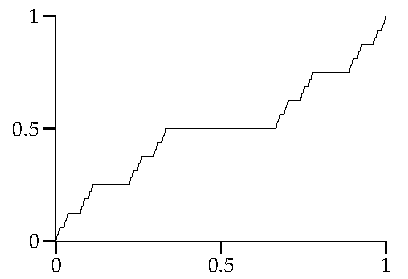
\includegraphics{figures/cantorfunction}
\caption{Cantor function or Devil's staircase (the function $\varphi$ from
the exercise).\label{fig:cantorfunction}}
\end{myfigureht}

\begin{exercise} \label{exercise:allowfiniteseqsinoutermeasure}
Prove that we obtain the same outer measure if we allow both finite and
infinite sequences in
the definition.  That is, define $\mu^*(S) := \inf\, \sum_{j \in I} V(R_j)$
where the infimum is taken over all countable (finite or infinite) sets of
open rectangles $\{ R_j \}_{j\in I}$ such that $S \subset
\bigcup_{j \in I} R_j$.  Prove that for every $S \subset \R^n$,
$\mu^*(S) = m^*(S)$.
\end{exercise}


%%%%%%%%%%%%%%%%%%%%%%%%%%%%%%%%%%%%%%%%%%%%%%%%%%%%%%%%%%%%%%%%%%%%%%%%%%%%%%

\sectionnewpage
\section{The set of Riemann integrable functions }
\label{sec:riemannlebesgue}

\sectionnotes{1 lecture}

\subsection{Oscillation and continuity}

Consider
$S \subset \R^n$ and $f \colon S \to \R$.
Instead of just saying that $f$ is or is not continuous at
a point $x \in S$,
we want to quantify how discontinuous $f$ is 
at $x$.  For every $\delta > 0$, define the \emph{oscillation} of 
$f$ on the $\delta$-ball in subspace topology,
$B_S(x,\delta) = B_{\R^n}(x,\delta) \cap S$, as
\glsadd{not:oscillation}
\begin{equation*}
o(f,x,\delta) :=
{\sup_{y \in B_S(x,\delta)} f(y)}
-
{\inf_{y \in B_S(x,\delta)} f(y)}
= 
\sup_{y_1,y_2 \in B_S(x,\delta)} \bigl(f(y_1)-f(y_2)\bigr) .
\end{equation*}
That is, $o(f,x,\delta)$ is the length of the smallest interval
that contains the image $f\bigl(B_S(x,\delta)\bigr)$.
Clearly $o(f,x,\delta) \geq 0$ and
$o(f,x,\delta) \leq o(f,x,\delta')$ whenever $\delta < \delta'$.
Therefore, the limit as $\delta \to 0$ from the right exists, and
we define the \emph{\myindex{oscillation}} of $f$
at $x$ as
\begin{equation*}
o(f,x) :=
\lim_{\delta \to 0^+}
o(f,x,\delta) =
\inf_{\delta > 0}
o(f,x,\delta) .
\end{equation*}

\begin{prop}
A function
$f \colon S \to \R$ is continuous at $x \in S$ if and only if $o(f,x) = 0$.
\end{prop}

\begin{proof}
First suppose that $f$ is continuous at $x \in S$.  Given any $\epsilon > 0$,
there exists a $\delta > 0$ such that for $y \in B_S(x,\delta)$,
we have $\sabs{f(x)-f(y)} < \epsilon$.  Therefore, if $y_1,y_2 \in
B_S(x,\delta)$, then
\begin{equation*}
f(y_1)-f(y_2) =
\bigl(f(y_1)-f(x)\bigr)-\bigl(f(y_2)-f(x)\bigr) < \epsilon + \epsilon = 2 \epsilon .
\end{equation*}
We take the supremum over $y_1$ and $y_2$
\begin{equation*}
o(f,x,\delta) = 
\sup_{y_1,y_2 \in B_S(x,\delta)} \bigl(f(y_1)-f(y_2)\bigr)
\leq
2 \epsilon .
\end{equation*}
As $o(x,f) \leq o(f,x,\delta) \leq 2\epsilon$, and $\epsilon > 0$ was arbitrary,
$o(x,f) = 0$.

On the other hand suppose $o(x,f) = 0$.  Given any $\epsilon > 0$,
find a $\delta > 0$ such that $o(f,x,\delta) < \epsilon$.  If
$y \in B_S(x,\delta)$, then
\begin{equation*}
\sabs{f(x)-f(y)}
\leq
\sup_{y_1,y_2 \in B_S(x,\delta)} \bigl(f(y_1)-f(y_2)\bigr)
=
o(f,x,\delta) < \epsilon. \qedhere
\end{equation*}
\end{proof}

\begin{prop} \label{prop:seclosed}
Let $S \subset \R^n$ be closed,
$f \colon S \to \R$, and $\epsilon > 0$.
The set $\bigl\{ x \in S : o(f,x) \geq \epsilon \bigr\}$ is closed.
\end{prop}

\begin{proof}
Equivalently, we want to show that
$G = \bigl\{ x \in S : o(f,x) < \epsilon \bigr\}$ is open in the subspace topology.
As $\inf_{\delta > 0} o(f,x,\delta) < \epsilon$, find a $\delta > 0$ such
that
\begin{equation*}
o(f,x,\delta) < \epsilon
\end{equation*}
Take any $\xi \in B_S(x,\nicefrac{\delta}{2})$.  Notice that
$B_S(\xi,\nicefrac{\delta}{2}) \subset B_S(x,\delta)$.  Therefore,
\begin{equation*}
o(f,\xi,\nicefrac{\delta}{2}) =
\sup_{y_1,y_2 \in B_S(\xi,\nicefrac{\delta}{2})} \bigl(f(y_1)-f(y_2)\bigr) 
\leq
\sup_{y_1,y_2 \in B_S(x,\delta)} \bigl(f(y_1)-f(y_2)\bigr) = o(f,x,\delta) <
\epsilon .
\end{equation*}
So $o(f,\xi) < \epsilon$ as well.  As this is true for all $\xi \in
B_S(x,\nicefrac{\delta}{2})$, we get that $G$ is open in the subspace
topology and $S \setminus G$ is closed as claimed.
\end{proof}


\subsection{The set of Riemann integrable functions}

We have seen that continuous functions are Riemann integrable, but we also
know that certain kinds of discontinuities are allowed.
It turns out that as long as the discontinuities happen on a set of measure
zero, the function is integrable, and vice versa.

\begin{thm}[Riemann--Lebesgue]\index{Riemann--Lebesgue theorem}
Let $R \subset \R^n$ be a closed rectangle and $f \colon R \to \R$
a bounded function.  Then $f$ is Riemann integrable if and only if
the set of discontinuities of $f$ is of measure zero (a null set).
\end{thm}

\begin{proof}
Let $S \subset R$ be the set of discontinuities of $f$, that is,
$S = \bigl\{ x \in R : o(f,x) > 0 \bigr\}$.
Suppose $S$ is a measure zero set: $m^*(S) = 0$.
The trick to this proof is to isolate the
bad set into a small set of subrectangles of a partition.  There are only
finitely many subrectangles of a partition, so we will wish to use
compactness.  If $S$ were closed, then it would be compact and we could cover
it by finitely many small rectangles as it is of measure zero.  Unfortunately, $S$
is not closed in general, so we need to work a little harder.

For every $\epsilon > 0$, define
\begin{equation*}
S_\epsilon := \bigl\{ x \in R : o(f,x) \geq \epsilon \bigr\} .
\end{equation*}
By \propref{prop:seclosed}, $S_\epsilon$ is closed and as it is a subset of
$R$,
which is bounded, $S_\epsilon$ is compact.  Furthermore,
$S_\epsilon \subset S$ and $S$ is of measure zero, so $S_\epsilon$ is
measure zero.
Via \propref{mv:prop:compactnull} finitely many open rectangles
$O_1,O_2,\ldots,O_k$ cover $S_\epsilon$ and
$\sum V(O_j) < \epsilon$.  

The set $T = R \setminus ( O_1 \cup \cdots \cup O_k )$ is closed, bounded,
and therefore compact.  Furthermore, $o(f,x) < \epsilon$ for all $x \in T$.
Hence for each $x \in T$, there exists a small closed rectangle
$T_x$ with $x$ in the interior of $T_x$, such that
\begin{equation*}
\sup_{y\in T_x} f(y) - \inf_{y\in T_x} f(y) < 2\epsilon.
\end{equation*}
The interiors of the rectangles $T_x$ cover $T$.  As $T$ is compact,
finitely many such rectangles $T_1, T_2, \ldots, T_m$
cover $T$.

Take the rectangles $T_1,T_2,\ldots,T_m$ and $O_1,O_2,\ldots,O_k$
and construct a partition out of their endpoints.  That is, construct
a partition $P$ of $R$ with subrectangles $R_1,R_2,\ldots,R_p$
such that every $R_j$ is contained in $T_\ell$ for some $\ell$
or the closure of $O_\ell$ for some $\ell$.  Order
the rectangles so that $R_1,R_2,\ldots,R_q$ are those
that are contained in some $T_\ell$, and $R_{q+1},R_{q+2},\ldots,R_{p}$
are the rest.
In particular,
\begin{equation*}
\sum_{j=1}^q V(R_j) \leq V(R)
\qquad \text{and} \qquad
\sum_{j=q+1}^p V(R_j) \leq \epsilon .
\end{equation*}
Let $m_j$ and $M_j$ be the inf and sup
of $f$
over $R_j$ as before.
If $R_j \subset T_\ell$ for some $\ell$, then $(M_j-m_j) < 2 \epsilon$.
Let $B \in \R$ be such that
$\sabs{f(x)} \leq B$ for all $x \in R$, so $(M_j-m_j) < 2B$ over all
rectangles. Then
\begin{equation*}
\begin{split}
U(P,f)-L(P,f)
& =
\sum_{j=1}^p (M_j-m_j) V(R_j)
\\
& =
\left(
\sum_{j=1}^q (M_j-m_j) V(R_j)
\right)
+
\left(
\sum_{j=q+1}^p (M_j-m_j) V(R_j)
\right)
\\
& \leq
\left(
\sum_{j=1}^q 2\epsilon\, V(R_j)
\right)
+
\left(
\sum_{j=q+1}^p 2 B\, V(R_j)
\right)
\\
& \leq
2 \epsilon\, V(R)
+
2B \epsilon = \epsilon \bigl(2\, V(R)+2B\bigr) .
\end{split}
\end{equation*}
We can make the right-hand side as small as we want,
and hence $f$ is integrable.

\medskip

For the other direction, suppose $f$ is Riemann integrable
on $R$.
Let $S$ be the set of discontinuities again.  Consider
the sequence of sets
\begin{equation*}
S_{1/k} = \bigl\{ x \in R : o(f,x) \geq \nicefrac{1}{k} \bigr\}.
\end{equation*}
Fix a $k \in \N$.
Given an $\epsilon > 0$, find a partition $P$ with subrectangles
$R_1,R_2,\ldots,R_p$ such that
\begin{equation*}
U(P,f)-L(P,f) =
\sum_{j=1}^p (M_j-m_j) V(R_j)
< \epsilon
\end{equation*}
Suppose $R_1,R_2,\ldots,R_p$ are ordered so that
the interiors of $R_1,R_2,\ldots,R_{q}$ intersect $S_{1/k}$,
while the interiors of $R_{q+1},R_{q+2},\ldots,R_p$
are disjoint from $S_{1/k}$.  If $x \in R_j \cap S_{1/k}$
and $x$ is in the interior of $R_j$,
%so sufficiently small balls are completely inside $R_j$,
then by definition of $S_{1/k}$ we have
$M_j-m_j \geq \nicefrac{1}{k}$.
Then
\begin{equation*}
\epsilon >
\sum_{j=1}^p (M_j-m_j) V(R_j)
\geq
\sum_{j=1}^q (M_j-m_j) V(R_j)
\geq
\frac{1}{k}
\sum_{j=1}^q V(R_j)
\end{equation*}
In other words,
$\sum_{j=1}^q V(R_j) < k \epsilon$.
Let $G$ be the set of all boundaries of all the subrectangles
of $P$.  The set $G$ is of measure zero (see \exampleref{mv:example:planenull}).
Let $R_j^\circ$ denote the interior of $R_j$, then
\begin{equation*}
S_{1/k} \subset R_1^\circ \cup R_2^\circ \cup \cdots \cup R_q^\circ \cup G .
\end{equation*}
As $G$ can be covered by open rectangles arbitrarily small volume,
$S_{1/k}$ must be of measure zero.  As
\begin{equation*}
S = \bigcup_{k=1}^\infty S_{1/k}
\end{equation*}
and a countable union of measure zero sets is of measure zero, 
$S$ is of measure zero.
\end{proof}

\begin{cor} \label{cor:closednessofriemannintegrable}
Let $R \subset \R^n$ be a closed rectangle.  Let $\sR(R)$ be the set
of Riemann integrable functions on $R$.  Then
\begin{enumerate}[(i)]
\item
$\sR(R)$ is a real algebra:
If $f,g \in \sR(R)$ and $a \in \R$, then $af \in \sR(R)$, $f+g \in \sR(R)$
and $fg \in \sR(R)$.
\item
If $f,g \in \sR(R)$ and
\begin{equation*}
\varphi(x) := \max \bigl\{ f(x) , g(x) \bigr\} ,
\qquad
\psi(x) := \min \bigl\{ f(x) , g(x) \bigr\} ,
\end{equation*}
then $\varphi, \psi \in \sR(R)$.
\item
If $f \in \sR(R)$, then $\sabs{f} \in \sR(R)$, where $\sabs{f}(x) :=
\sabs{f(x)}$.
\item
If $R' \subset \R^m$ is another closed rectangle,
$U \subset \R^n$ and $U' \subset \R^m$ are open sets such that
$R \subset U$ and $R' \subset U'$,
$g \colon U \to U'$ is continuously differentiable, bijective,
$g^{-1}$ is continuously differentiable,
and $f \in \sR(R')$,
then the composition $f \circ g$ is Riemann integrable on $R$.
\end{enumerate}
\end{cor}

The proof is contained in the exercises.

\subsection{Exercises}

\begin{exercise}
Suppose $f \colon (a,b) \times (c,d) \to \R$ is a bounded continuous
function.  Show that the integral of $f$ over $R = [a,b] \times [c,d]$ makes sense
and is uniquely defined.  That is, set $f$ to be anything on the boundary of
$R$ and compute the integral, showing that the values on the boundary are
irrelevant.
\end{exercise}

\begin{exercise}
Suppose $R \subset \R^n$ is a closed rectangle.  Show that $\sR(R)$, the set
of Riemann integrable functions, is an algebra.  That is, show that
if $f,g \in \sR(R)$ and $a \in \R$, then $af \in \sR(R)$, $f+g \in \sR(R)$,
and $fg \in \sR(R)$.
\end{exercise}

\begin{exercise}
Suppose $R \subset \R^n$ is a closed rectangle and
$f \colon R \to \R$ is a bounded function which is zero except on a closed set $E
\subset R$ of measure
zero.  Show that $\int_R f$ exists and compute it.
\end{exercise}

\begin{exercise}
Suppose $R \subset \R^n$ is a closed rectangle and
$f \colon R \to \R$ and
$g \colon R \to \R$ are two Riemann integrable functions.  Suppose $f = g$
except for a closed set $E \subset R$ of measure zero.  Show that $\int_R f = \int_R g$.
\end{exercise}

\begin{samepage}
\begin{exercise}
Suppose $R \subset \R^n$ is a closed rectangle and
$f \colon R \to \R$ is a bounded function.
\begin{enumerate}[a)]
\item
Suppose there exists a closed set $E \subset R$ of measure zero such that
$f|_{R\setminus E}$ is continuous.  Then $f \in \sR(R)$.
\item
Find an example where $E \subset R$ is a set of measure zero
(not closed) such that
$f|_{R\setminus E}$ is continuous and $f \not\in \sR(R)$.
\end{enumerate}
\end{exercise}
\end{samepage}

\begin{exercise}
Suppose $R \subset \R^n$ is a closed rectangle
and $f \colon R \to \R$ and $g \colon R \to \R$ 
are Riemann integrable.
Show that
\begin{equation*}
\varphi(x) := \max \bigl\{ f(x) , g(x) \bigr\} ,
\qquad
\psi(x) := \min \bigl\{ f(x) , g(x) \bigr\} ,
\end{equation*}
are Riemann integrable.
\end{exercise}

\begin{exercise}
Suppose $R \subset \R^n$ is a closed rectangle
and $f \colon R \to \R$ is Riemann integrable.
Show that $\sabs{f}$ is Riemann integrable.
Hint: Define
$f_+(x) := \max \bigl\{ f(x) , 0 \bigr\}$ and
$f_-(x) := \max \bigl\{ -f(x) , 0 \bigr\}$, and then write $\sabs{f}$
in terms of $f_+$ and $f_-$.
\end{exercise}

\begin{exercise}
\leavevmode
\begin{enumerate}[a)]
\item
Suppose $R \subset \R^n$ and
$R' \subset \R^m$ are closed rectangles,
$U \subset \R^n$ and $U' \subset \R^m$ are open sets such that
$R \subset U$ and $R' \subset U'$,
$g \colon U \to U'$ is continuously differentiable, bijective,
$g^{-1}$ is continuously differentiable, and
$f \in \sR(R')$, 
then the composition $f \circ g$ is Riemann integrable on $R$.
\item
Find a counterexample when $g$ is not one-to-one.
Hint: Try $g(x,y) := (x,0)$ and $R=R'=[0,1] \times [0,1]$.
\end{enumerate}
\end{exercise}

\begin{exercise}
Suppose 
$f \colon [0,1]^2 \to \R$ is defined by
\begin{equation*}
f(x,y) :=
\begin{cases}
\frac{1}{kq} & \text{if } x,y \in \Q \text{ and } x = \frac{\ell}{k}
\text{ and } y=\frac{p}{q} \text{ in lowest terms,} \\
0            & \text{else.}
\end{cases}
\end{equation*}
Show that $f \in \sR\bigl({[0,1]}^2\bigr)$.
\end{exercise}

\begin{exercise}
Compute the oscillation $o\bigl(f,(x,y)\bigr)$ for all $(x,y) \in \R^2$
for the function
\begin{equation*}
f(x,y) :=
\begin{cases}
\frac{xy}{x^2+y^2} & \text{if } (x,y) \not= (0,0), \\
0                  & \text{if } (x,y) = (0,0) .
\end{cases}
\end{equation*}
\end{exercise}

\begin{exercise}
Consider the popcorn function $f \colon [0,1] \to \R$,
\begin{equation*}
f(x) :=
\begin{cases}
\frac{1}{q} & \text{if } x \in \Q \text{ and } x = \frac{p}{q}
 \text{ in lowest terms,} \\
0           & \text{else.}
\end{cases}
\end{equation*}
Compute $o(f,x)$ for all $x \in [0,1]$.
\end{exercise}


%%%%%%%%%%%%%%%%%%%%%%%%%%%%%%%%%%%%%%%%%%%%%%%%%%%%%%%%%%%%%%%%%%%%%%%%%%%%%%

\sectionnewpage
\section{Jordan measurable sets}
\label{sec:jordansets}

\sectionnotes{1 lecture}

\subsection{Volume and Jordan measurable sets}

Given a set
$S \subset \R^n$, its \emph{\myindex{characteristic function}}
or \emph{\myindex{indicator function}} $\chi_S \colon \R^n \to \R$
is defined by
\glsadd{not:indicatorfunction}
\begin{equation*}
\chi_S(x) :=
\begin{cases}
1 & \text{if } x \in S, \\
0 & \text{if } x \notin S.
\end{cases}
\end{equation*}
A bounded set $S$ is \emph{\myindex{Jordan measurable}}\footnote{Named after
the French mathematician
\href{https://en.wikipedia.org/wiki/Camille_Jordan}{Marie Ennemond Camille Jordan}
(1838--1922).}
if for some closed rectangle $R$ such that $S \subset R$, the function
$\chi_S$ is Riemann integrable, that is, $\chi_S \in \sR(R)$.
Take two closed rectangles $R$ and $R'$ 
with $S \subset R$ and $S \subset R'$, then $R \cap R'$ is a closed rectangle
also containing $S$.  By \propref{mv:prop:integralsmallerset}
and \exerciseref{mv:zerooutside}, $\chi_S \in \sR(R \cap R')$
and so $\chi_S \in \sR(R')$.  Thus
\begin{equation*}
\int_R \chi_S = \int_{R'} \chi_S = \int_{R \cap R'} \chi_S.
\end{equation*}
We define the
\emph{$n$-dimensional volume}%
\index{n-dimensional volume@$n$-dimensional volume!Jordan measurable set}%
\index{volume} of the
bounded Jordan measurable set $S$ as
\glsadd{not:ndimvolume}
\begin{equation*}
V(S) := \int_R \chi_S ,
\end{equation*}
where $R$ is any closed rectangle containing $S$.

\begin{prop}
A bounded set $S \subset \R^n$ is Jordan measurable if and only if
the boundary $\partial S$ is a measure zero set.
\end{prop}

\begin{proof}
Suppose $R$ is a closed rectangle such that $S$ is
contained in the interior of $R$.
If $x \in \partial S$, then for every $\delta > 0$,
the sets $S \cap B(x,\delta)$ (where $\chi_S$ is 1) and
the sets $(R \setminus S) \cap B(x,\delta)$ (where $\chi_S$ is 0) are
both nonempty.  So $\chi_S$ is not continuous at $x$.
If $x$ is either in the interior of $S$ or in the complement of the closure
$\widebar{S}$, then $\chi_S$ is either identically 1 or identically 0
in a whole neighborhood of $x$ and hence $\chi_S$ is continuous at $x$.
Therefore, the set of discontinuities of $\chi_S$ is precisely the
boundary $\partial S$.  The proposition follows.
\end{proof}

\begin{prop} \label{prop:jordanmeas}
Suppose $S$ and $T$ are bounded Jordan measurable sets.
Then
\begin{enumerate}[(i)]
\item The closure $\widebar{S}$ is Jordan measurable.
\item The interior $S^\circ$ is Jordan measurable.
\item $S \cup T$ is Jordan measurable.
\item $S \cap T$ is Jordan measurable.
\item $S \setminus T$ is Jordan measurable.
\end{enumerate}
\end{prop}

The proof of the proposition is left as an exercise.
Next, we find that the volume that we defined above coincides with the outer
measure we defined above.

\begin{prop}
If $S \subset \R^n$ is Jordan measurable, then $V(S) = m^*(S)$.
\end{prop}

\begin{proof}
Given $\epsilon > 0$,
let $R$ be a closed rectangle that contains $S$.  Let $P$ be a partition
of $R$ such that 
\begin{equation*}
U(P,\chi_S) \leq \left( \int_R \chi_S \right) + \epsilon = V(S) + \epsilon
\qquad \text{and} \qquad
L(P,\chi_S) \geq \left( \int_R \chi_S \right) - \epsilon = V(S)-\epsilon.
\end{equation*}
Let $R_1,R_2,\ldots,R_k$ be all the subrectangles of $P$ such that $\chi_S$ is not
identically zero on each $R_j$.  That is, there is some point $x \in R_j$ such
that $x \in S$.  Let $O_j$ be an open rectangle such that $R_j \subset O_j$
and $V(O_j) < V(R_j) + \nicefrac{\epsilon}{k}$.  Notice that $S \subset
\bigcup_j O_j$.  Then
\begin{equation*}
U(P,\chi_S) = \sum_{j=1}^k V(R_j) > 
\left(\sum_{j=1}^k V(O_j)\right) - \epsilon \geq m^*(S) - \epsilon .
\end{equation*}
As 
$U(P,\chi_S) \leq V(S) + \epsilon$, then
$m^*(S) - \epsilon \leq V(S) + \epsilon$, or in other words
$m^*(S) \leq V(S)$.

Let $R'_1,R'_2,\ldots,R'_\ell$ be all the subrectangles of $P$ such that
$\chi_S$ is identically one on each $R'_j$.  In other words,
these are the subrectangles contained in $S$.
  The interiors
of the subrectangles $R'^\circ_j$ are disjoint and
$V(R'^\circ_j) = V(R'_j)$.  It is easy to see from definition
that 
\begin{equation*}
m^*\Bigl(\bigcup_{j=1}^\ell R'^\circ_j\Bigr)
=
\sum_{j=1}^\ell
V(R'^\circ_j) .
\end{equation*}
Hence
\begin{equation*}
m^*(S) \geq
m^*\Bigl(\bigcup_{j=1}^\ell R'_j\Bigr)
\geq
m^*\Bigl(\bigcup_{j=1}^\ell R'^\circ_j\Bigr)
=
\sum_{j=1}^\ell
V(R'^\circ_j)
=
\sum_{j=1}^\ell
V(R'_j)
=
L(P,f) \geq V(S) - \epsilon .
\end{equation*}
Therefore $m^*(S) \geq V(S)$ as well.
\end{proof}

\subsection{Integration over Jordan measurable sets}

In $\R$ there is only one reasonable type of set to integrate over:
an interval.   In $\R^n$ there are many kinds of sets.  The ones
that work with the Riemann integral are the Jordan measurable sets.

\begin{defn}
Let $S \subset \R^n$ be a bounded Jordan measurable set.
A bounded function $f \colon S \to \R$
is said to be
\emph{\myindex{Riemann integrable on $S$}}\index{integrable on $S$},
or\glsadd{not:integrablefuncR} $f \in \sR(S)$, if for a closed
rectangle $R$ such that $S \subset R$, the function $\widetilde{f} \colon R
\to \R$ defined by
\begin{equation*}
\widetilde{f}(x) :=
\begin{cases}
f(x) & \text{if } x \in S, \\
0 & \text{otherwise},
\end{cases}
\end{equation*}
is in $\sR(R)$.  In this case we write
\glsadd{not:riemannintR}%
\begin{equation*}
\int_S f := \int_R \widetilde{f}.
\end{equation*}
\end{defn}

When $f$ is defined on a larger set and we wish to integrate over $S$, then
we apply the definition to the restriction $f|_S$.  In particular, 
if $f \colon R \to \R$ for a closed rectangle $R$, and $S \subset R$ is
a Jordan measurable subset, then
\begin{equation*}
\int_S f = \int_R f \chi_S .
\end{equation*}

\begin{prop}
If $S \subset \R^n$ is a bounded Jordan measurable set and $f \colon S \to \R$
is a bounded continuous function, then $f$ is integrable on $S$.
\end{prop}

\begin{proof}
Define the function $\widetilde{f}$ as above for some closed rectangle $R$ with $S
\subset R$.  If $x \in R \setminus \widebar{S}$, then $\widetilde{f}$
is identically zero in a neighborhood of $x$.  Similarly if $x$ is in the
interior of $S$, then $\widetilde{f} = f$ on a neighborhood of $x$
and $f$ is continuous at $x$.  Therefore, $\widetilde{f}$ is only ever
possibly discontinuous at $\partial S$, which is a set of measure zero,
and we are finished.
\end{proof}

\subsection{Images of Jordan measurable subsets}

Finally, images of Jordan measurable sets are Jordan measurable under
nice enough mappings.  For simplicity, we assume that the Jacobian
determinant never vanishes.

\begin{prop} \label{prop:imagejordanmeas}
Suppose $U \subset \R^n$ is open and
$S \subset U$ is a closed bounded Jordan measurable set.
Suppose
$g \colon U \to \R^n$ is a one-to-one
continuously differentiable mapping such that
the Jacobian determinant $J_g$ is never zero on $S$.
Then $g(S)$ is bounded and Jordan measurable.
\end{prop}

\begin{proof}
Let $T := g(S)$.  As $S \subset \R^n$ is closed and bounded it is compact.
By 
\volIref{\lemmaref*{vI-lemma:continuouscompact} from volume I}{\lemmaref{lemma:continuouscompact}},
the set
$T$ is also compact and so closed and bounded.
We claim $\partial T \subset g(\partial S)$.  Suppose the claim is proved.
As $S$ is Jordan measurable, then
$\partial S$ is measure zero.  Then  $g(\partial S)$ is measure
zero by \propref{prop:imagenull}.  As $\partial T \subset g(\partial
S)$, then $T$ is Jordan measurable.

It is therefore left to prove the claim.
As $T$ is closed, $\partial T \subset T$.
Suppose $y \in \partial T$, then there must exist an
$x \in S$
such that $g(x) = y$, and by hypothesis $J_g(x) \not= 0$.
We use the inverse function theorem (\thmref{thm:inverse}).  We find 
a neighborhood $V \subset U$ of $x$ and an open set $W$ such that
the restriction $f|_V$ is a one-to-one and onto function from $V$ to $W$
with a continuously differentiable inverse.  In particular, $g(x) = y \in W$.
As $y \in \partial T$, there exists a sequence $\{ y_k \}$ in $W$ with
$\lim y_k = y$ and $y_k \notin T$.  As $g|_V$ is invertible and in
particular has a continuous inverse, there exists
a sequence $\{ x_k \}$ in $V$ such that $g(x_k) = y_k$ and $\lim x_k = x$.
Since $y_k \notin T = g(S)$, clearly $x_k \notin S$.  Since $x \in S$, we
conclude that $x \in \partial S$.  The claim is proved, $\partial T \subset
g(\partial S)$.
\end{proof}

\subsection{Exercises}

\begin{exercise}
Prove \propref{prop:jordanmeas}.
\end{exercise}

\begin{exercise}
Prove that a bounded convex set is Jordan measurable.  Hint: Induction on
dimension.
\end{exercise}

\begin{samepage}
\begin{exercise} \label{exercise:intovertypeIset}
Let $f \colon [a,b] \to \R$ and
$g \colon [a,b] \to \R$ be continuous functions and such that
for all $x \in (a,b)$, $f(x) < g(x)$.  Let
\begin{equation*}
U := \bigl\{ (x,y) \in \R^2 : a < x < b \text{ and } f(x) < y < g(x) \bigr\} .
\end{equation*}
\begin{enumerate}[a)]
\item
Show that $U$ is Jordan measurable.
\item
If $\varphi \colon U \to \R$ is Riemann integrable on $U$, then
\begin{equation*}
\int_U \varphi =
\int_a^b \int_{g(x)}^{f(x)} \varphi(x,y) ~ dy ~ dx .
\end{equation*}
\end{enumerate}
\end{exercise}
\end{samepage}

\begin{exercise}
Let us construct an example of a non-Jordan measurable open set.
Start in one dimension.  Let $\{ r_j \}$ be an enumeration
of all rational numbers in $(0,1)$.  Let $(a_j,b_j)$ be open intervals
such that $(a_j,b_j) \subset (0,1)$ for all $j$, $r_j \in (a_j,b_j)$,
and $\sum_{j=1}^\infty (b_j-a_j) < \nicefrac{1}{2}$.  Now let $U :=
\bigcup_{j=1}^\infty (a_j,b_j)$.
\begin{enumerate}[a)]
\item
Show the open intervals $(a_j,b_j)$ as above actually exist.
\item
Prove $\partial U = [0,1] \setminus U$.
\item
Prove $\partial U$ is not of measure zero, and therefore $U$ is not Jordan measurable.
\item
Show that $W :=
\bigl( U \times (0,2) \bigr) \cup \bigl( (0,1) \times (1,2) \bigr)$
is a connected bounded open set in $\R^2$
that is not Jordan measurable.
\end{enumerate}
\end{exercise}

\begin{exercise}
Suppose $K \subset \R^n$ is a closed measure zero set.
\begin{enumerate}[a)]
\item
If $K$ is bounded, prove that $K$ is Jordan measurable.
\item
If $S \subset \R^n$ is bounded and Jordan measurable, prove that
$S \setminus K$ is Jordan measurable.
\item
Construct a bounded Jordan measurable $S \subset \R^n$
and a bounded $T \subset \R^n$ of measure zero, such that
neither $T$ nor $S \setminus T$ is Jordan measurable.
\end{enumerate}
\end{exercise}

\begin{exercise}
Suppose $U \subset \R^n$ is open and $K \subset U$ is compact.
Find a compact Jordan measurable set $S$ such that $S \subset U$
and $K \subset S^\circ$ ($K$ is in the interior of $S$).
\end{exercise}

\begin{exercise} \label{exercise:closednessofriemannintegrable}
Prove a version of \corref{cor:closednessofriemannintegrable}, replacing all closed
rectangles with bounded Jordan measurable sets.
\end{exercise}

%%%%%%%%%%%%%%%%%%%%%%%%%%%%%%%%%%%%%%%%%%%%%%%%%%%%%%%%%%%%%%%%%%%%%%%%%%%%%%

\sectionnewpage
\section{Green's theorem}
\label{sec:mvgreenstheorem}

\sectionnotes{1 lecture, requires \chapterref{path:chapter}}

One of the most important theorems of analysis in several variables is the
so-called generalized Stokes' theorem, a generalization of the
fundamental theorem of calculus.  The two-dimensional
version is called Green's theorem%
\footnote{Named after the British mathematical physicist
\href{https://en.wikipedia.org/wiki/George_Green_(mathematician)}{George Green}
(1793--1841).}.  We will state the theorem in general, but
we will only prove a special, but important, case.

\begin{defn}
Let $U \subset \R^2$ be a bounded connected open set.
Suppose the boundary
$\partial U$ is a disjoint union of (the images of) finitely many
simple closed piecewise smooth paths such that
every $p \in \partial U$ is in the closure of
$\R^2 \setminus \widebar{U}$.
Then $U$ is called a
\emph{\myindex{bounded domain with piecewise smooth boundary}}%
\index{piecewise smooth boundary}
in $\R^2$.
\end{defn}

The condition about points outside the closure says that locally $\partial U$
separates $\R^2$ into an \myquote{inside} and an \myquote{outside.}  The condition prevents
$\partial U$ from being just a \myquote{cut} inside $U$.  As we travel
along the path in a certain orientation,
there is a well-defined left and a right, and either $U$ is on the left
and the complement of $U$ is on the right, or vice versa.   
The orientation on $U$ is the direction in which we travel along the
paths.  We can switch orientation if needed by reparametrizing the
path.

\begin{defn}
Let $U \subset \R^2$ be a bounded domain with piecewise smooth boundary,
let $\partial U$ be oriented ,
and let $\gamma \colon [a,b] \to \R^2$ be a parametrization of $\partial U$
giving the orientation.  Write $\gamma(t) = \big(x(t),y(t)\bigr)$.
If the vector $n(t) := \bigl(-y'(t),x'(t)\bigr)$ points into the domain,
that is, $\epsilon n(t) + \gamma(t)$ is in $U$ for all small enough
$\epsilon > 0$, then $\partial U$ is
\emph{\myindex{positively oriented}}.  
See \figureref{fig:positiveorient}.
Otherwise it is \emph{\myindex{negatively oriented}}.
\end{defn}

\begin{myfigureht}
\subimport*{figures/}{positiveorient.pdf_t}
\caption{Positively oriented domain (left), and a positively oriented
domain with a hole (right).\label{fig:positiveorient}}
\end{myfigureht}


The vector $n(t)$ turns $\gamma^{\:\prime}(t)$
counterclockwise by $90^\circ$, that is to the left.
When we travel along a positively oriented boundary
in the direction of its orientation,
the domain is \myquote{on our left.}
For example,
if $U$ is a bounded domain with \myquote{no holes,} that is $\partial U$
is connected, then the positive orientation means we are traveling
counterclockwise around $\partial U$.  If we do have \myquote{holes,} then we
travel around them clockwise.

\begin{prop}
Let $U \subset \R^2$ be a bounded domain with piecewise smooth boundary.
Then $U$ is Jordan measurable.
\end{prop}

\begin{proof}
We must show that
$\partial U$ is a null set.  As $\partial U$ is a finite
union of piecewise smooth paths, which 
are finite unions of smooth paths, we need only show that 
a smooth path in $\R^2$ is a null set.
Let $\gamma \colon [a,b] \to \R^2$ be a smooth path.
It is enough to show that
$\gamma\bigl((a,b)\bigr)$ is a null set, as adding 
the points $\gamma(a)$ and $\gamma(b)$,
to a null set still results in a null set.
Define
\begin{equation*}
f \colon (a,b) \times (-1,1) \to \R^2,
\qquad \text{as} \qquad
f(x,y) := \gamma(x) .
\end{equation*}
The set $(a,b) \times \{ 0 \}$ is a null set in $\R^2$ and
$\gamma\bigl((a,b)\bigr) = f\bigl( (a,b) \times \{ 0 \} \bigr)$.
By \propref{prop:imagenull}, 
$\gamma\bigl((a,b)\bigr)$ is a null set in $\R^2$
and so
$\gamma\bigl([a,b]\bigr)$ is a null set, and 
so finally $\partial U$ is a null set.
\end{proof}

\begin{thm}[Green]\index{Green's theorem}
Suppose $U \subset \R^2$ is a bounded domain with piecewise smooth boundary with
the boundary positively oriented.  Suppose $P$ and $Q$ are continuously
differentiable functions defined on some open set that contains the closure
$\widebar{U}$.  Then
\begin{equation*}
\int_{\partial U}
P ~ dx + Q~  dy
=
\int_{U}
\left(\frac{\partial Q}{\partial x} - \frac{\partial P}{\partial y} \right)
.
\end{equation*}
\end{thm}

We stated Green's theorem in general, although we will only prove a special 
version of it.  That is, we will only prove it for a special kind of domain.
The general version follows from the special case 
by application of further geometry, and cutting up the general
domain into smaller domains on which to apply the special case.
We will not prove the general case. 

Let $U \subset \R^2$ be a domain with piecewise smooth boundary.
We say $U$ is of \emph{type I}\index{type I domain}
if there exist numbers
$a < b$, and continuous
functions $f \colon [a,b] \to \R$ and
$g \colon [a,b] \to \R$, such that
\begin{equation*}
U := \{ (x,y) \in \R^2 : a < x < b \text{ and } f(x) < y < g(x) \} .
\end{equation*}
Similarly, $U$ is of \emph{type II}\index{type II domain}
if there exist numbers
$c < d$, and continuous
functions $h \colon [c,d] \to \R$ and
$k \colon [c,d] \to \R$, such that
\begin{equation*}
U := \{ (x,y) \in \R^2 : c < y < d \text{ and } h(y) < x < k(y) \} .
\end{equation*}
Finally, $U \subset \R^2$ is of \emph{type III}\index{type III domain}
if it is both of type I and type II\@.  See \figureref{fig:greenstypes}.

\begin{myfigureht}
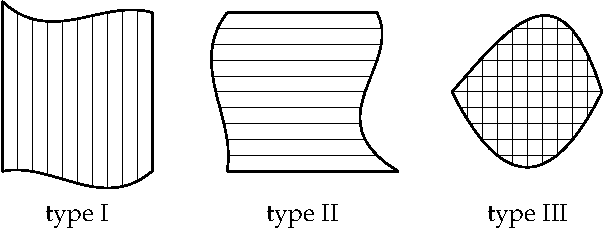
\includegraphics{figures/greenstypes}
\caption{Domain types for Green's theorem.\label{fig:greenstypes}}
\end{myfigureht}

Common domains to apply Green's theorem to are rectangles and discs, and
these are type III domains.
We will only prove Green's theorem for type III domains.

\begin{proof}[Proof of Green's theorem for $U$ of type III]
Let $f,g,h,k$ be the functions defined above.
Using \exerciseref{exercise:intovertypeIset},
$U$ is Jordan measurable and as $U$ is of type I\@, then
\begin{equation*}
\begin{split}
\int_U 
\left(- \frac{\partial P}{\partial y} \right)
& =
\int_a^b \int_{g(x)}^{f(x)}
\left(- \frac{\partial P}{\partial y} (x,y) \right)
~ dy ~ dx 
\\
& =
\int_a^b \Bigl(
- P\bigl(x,f(x)\bigr) +
P\bigl(x,g(x)\bigr)
\Bigr) ~ dx
\\
& =
\int_a^b P\bigl(x,g(x)\bigr) ~ dx 
-
\int_a^b P\bigl(x,f(x)\bigr) ~ dx .
\end{split}
\end{equation*}
We integrate $P~dx$ along the boundary.
The one-form $P~dx$ integrates to zero 
along the straight vertical lines in the boundary.  Therefore it is
only
integrated along the top and along the bottom.  As a parameter,
$x$ runs from left to right.  If we use the parametrizations that take $x$
to $\bigl(x,f(x)\bigr)$ and to
$\bigl(x,g(x)\bigr)$ we recognize path integrals above.  However the second
path integral is in the wrong direction; the top should be going right to
left, and so we must switch orientation.
\begin{equation*}
\int_{\partial U} P ~ dx
=
\int_a^b P\bigl(x,g(x)\bigr) ~ dx 
+
\int_b^a P\bigl(x,f(x)\bigr) ~ dx
=
\int_U 
\left(- \frac{\partial P}{\partial y} \right) .
\end{equation*}

Similarly, $U$ is also of type II\@.  The form $Q~dy$ integrates to zero along
horizontal lines.   So
\begin{equation*}
\int_U 
\frac{\partial Q}{\partial x}
=
\int_c^d \int_{k(y)}^{h(y)}
\frac{\partial Q}{\partial x}(x,y)
~ dx ~ dy 
=
\int_a^b \Bigl(
Q\bigl(y,h(y)\bigr) 
-
Q\bigl(y,k(y)\bigr)
\Bigr) ~ dx 
=
\int_{\partial U} Q ~ dy .
\end{equation*}
Putting the two together we obtain
\begin{equation*}
\int_{\partial U} P~ dx + Q ~ dy 
=
\int_{\partial U} P~ dx + \int_{\partial U} Q ~ dy 
=
\int_U 
\Bigl(-\frac{\partial P}{\partial y}\Bigr)
+
\int_U 
\frac{\partial Q}{\partial x}
=
\int_U 
\Bigl(
\frac{\partial Q}{\partial x}
-\frac{\partial P}{\partial y}
\Bigr) . \qedhere
\end{equation*}
\end{proof}

We illustrate the usefulness of Green's theorem on a fundamental result
about harmonic functions.

\begin{example}
Suppose $U \subset \R^2$ is open and
$f \colon U \to \R$ is harmonic, that is, $f$ is twice continuously
differentiable and
$\frac{\partial^2 f}{\partial x^2} +
\frac{\partial^2 f}{\partial y^2} = 0$.
We will prove one of the most fundamental properties of harmonic functions.

Let $D_r := B(p,r)$ be closed disc such that its closure $C(p,r) \subset U$.  Write
$p = (x_0,y_0)$.  We orient
$\partial D_r$ positively.  See \exerciseref{green:balltype3orient}.
Then
\begin{equation*}
\begin{split}
0
& =
\frac{1}{2\pi r}
\int_{D_r}
\left(
\frac{\partial^2 f}{\partial x^2} +
\frac{\partial^2 f}{\partial y^2}
\right)
\\
& 
=
\frac{1}{2\pi r}
\int_{\partial D_r}
- \frac{\partial f}{\partial y} ~ dx + 
\frac{\partial f}{\partial x} ~ dy
\\
&
=
\frac{1}{2\pi r}
\int_0^{2\pi}
\biggl(
- \frac{\partial f}{\partial y} \bigl(x_0+r\cos(t),y_0+r\sin(t)\bigr) \bigl(-r\sin(t)\bigr)
\\
& \hspace{1.2in}
+ \frac{\partial f}{\partial x} \bigl(x_0+r\cos(t),y_0+r\sin(t)\bigr) r\cos(t)
\biggr) ~ dt
\\
&
=
\frac{d}{dr}
\left[
\frac{1}{2\pi}
\int_0^{2\pi}
f\bigl(x_0+r\cos(t),y_0+r\sin(t)\bigr) ~ dt
\right] .
\end{split}
\end{equation*}
Let $g(r) := 
\frac{1}{2\pi}
\int_0^{2\pi}
f\bigl(x_0+r\cos(t),y_0+r\sin(t)\bigr) ~ dt$.  Then $g'(r) = 0$ for all
$r > 0$.
The function is constant for $r >0$ and continuous at $r=0$ (exercise).
Therefore, $g(0) = g(r)$ for all $r > 0$, and
\begin{equation*}
g(r) = g(0) = 
\frac{1}{2\pi}
\int_0^{2\pi}
f\bigl(x_0+0\cos(t),y_0+0\sin(t)\bigr) ~ dt
=
f(x_0,y_0).
\end{equation*}
We
proved the \emph{\myindex{mean value property}} of harmonic functions:
\begin{equation*}
f(x_0,y_0) = 
\frac{1}{2\pi}
\int_0^{2\pi}
f\bigl(x_0+r\cos(t),y_0+r\sin(t)\bigr) ~ dt 
=
\frac{1}{2\pi r}
\int_{\partial D_r} f ~ ds .
\end{equation*}
That is, the value at $p = (x_0,y_0)$ is the average over a circle of any
radius $r$ centered at $(x_0,y_0)$.
\end{example}

\subsection{Exercises}

\begin{exercise} \label{green:balltype3orient}
Prove that a disc $B(p,r) \subset \R^2$ is a type III domain, and prove that
the orientation given by the parametrization $\gamma(t) =
\bigl(x_0+r\cos(t),y_0+r\sin(t)\bigr)$ where $p = (x_0,y_0)$ is the positive
orientation of the boundary $\partial B(p,r)$.
\\
Note: Feel free to use what you know about sine and cosine from calculus.
\end{exercise}

\begin{exercise}
Prove that a convex bounded domain with piecewise smooth boundary
is a type III domain.
\end{exercise}

\begin{exercise}
Suppose $V \subset \R^2$ is a domain with piecewise smooth boundary that is
a type III domain and suppose that $U \subset \R^2$ is a domain such that
$\widebar{V} \subset U$.  Suppose $f \colon U \to \R$ is a twice
continuously differentiable function.  Prove that
$\int_{\partial V}
\frac{\partial f}{\partial x} dx + 
\frac{\partial f}{\partial y} dy = 0$.
\end{exercise}

\begin{samepage}
\begin{exercise}
For a disc $B(p,r) \subset \R^2$, orient the boundary $\partial B(p,r)$
positively.
\begin{enumerate}[a)]
\item
Compute $\displaystyle \int_{\partial B(p,r)} -y ~ dx$.
\item
Compute $\displaystyle \int_{\partial B(p,r)} x ~ dy$.
\item
Compute $\displaystyle \int_{\partial B(p,r)} \frac{-y}{2} ~ dx +
\frac{x}{2} ~ dy$.
\end{enumerate}
\end{exercise}
\end{samepage}

\begin{exercise}
Using Green's theorem show that the area of a triangle with
vertices
$(x_1,y_1)$,
$(x_2,y_2)$,
$(x_3,y_3)$ is
$\frac{1}{2}\sabs{x_1y_2 + x_2 y_3 + x_3 y_1 - y_1x_2 - y_2x_3 - y_3x_1}$.
Hint: See previous exercise.
\end{exercise}

\begin{exercise}
Using the mean value property prove the
\emph{maximum principle}\index{maximum principle!harmonic functions}
for harmonic functions:
Suppose $U \subset \R^2$ is a connected open set and
$f \colon U \to \R$ is harmonic. Prove that
if $f$ attains a maximum at $p \in U$, then $f$ is constant.
\end{exercise}

\begin{exercise}
Let $f(x,y) := \ln \sqrt{x^2+y^2}$.
\begin{enumerate}[a)]
\item
Show $f$ is harmonic where defined.
\item
Show $\lim_{(x,y) \to 0} f(x,y) = -\infty$.
\item
Using a circle $C_r$ of radius
$r$ around the origin, compute $\frac{1}{2\pi r} \int_{\partial C_r} f ds$.
What happens as $r \to 0$?
\item
Why can't you use Green's theorem?
\end{enumerate}
\end{exercise}


%%%%%%%%%%%%%%%%%%%%%%%%%%%%%%%%%%%%%%%%%%%%%%%%%%%%%%%%%%%%%%%%%%%%%%%%%%%%%%

\sectionnewpage
\section{Change of variables}
\label{sec:mvchangeofvars}

\sectionnotes{1 lecture}

In one variable, we have the familiar change of variables
\begin{equation*}
\int_a^b f\bigl(g(x)\bigr) g'(x)~ dx = 
\int_{g(a)}^{g(b)} f(x) ~ dx .
\end{equation*}
The analogue in higher dimensions is quite
a bit more complicated.  The first complication is orientation.  If we use
the definition of integral from this chapter, then we do not have the notion
of $\int_a^b$ versus $\int_b^a$.  We are simply integrating over an
interval $[a,b]$.  With this notation, the change of variables becomes
\begin{equation*}
\int_{[a,b]} f\bigl(g(x)\bigr) \sabs{g'(x)}~ dx = 
\int_{g([a,b])} f(x) ~ dx .
\end{equation*}
In this section we will obtain the several-variable analogue of this form.

Let us remark the role of $\sabs{g'(x)}$ in the formula. 
The integral measures volumes in general, so in one dimension it measures length.
Notice that $\sabs{g'(x)}$ scales the $dx$ and
so it scales the lengths.
If our $g$ is linear, that is, $g(x)=Lx$, then
$g'(x) = L$ and the length of the interval $g([a,b])$ is simply
$\sabs{L}(b-a)$.  That is because $g([a,b])$ is either $[La,Lb]$ or
$[Lb,La]$.  This property holds in higher dimension with $\sabs{L}$ replaced
by the absolute value of the determinant.

\begin{prop} \label{prop:volrectdet}
Suppose $R \subset \R^n$ is a rectangle
and $A \colon \R^n \to \R^n$ is linear.  Then
$A(R)$ is Jordan measurable and $V\bigl(A(R)\bigr) = \sabs{\det (A)} V(R)$.
\end{prop}

\begin{proof}
It is enough to prove for elementary matrices.  The proof is left as an
exercise.
\end{proof}

Let us prove that
absolute value of the Jacobian determinant
$\sabs{J_g(x)} = \babs{\det \bigl(g'(x)\bigr)}$
is the replacement of $\sabs{g'(x)}$ for multiple
dimensions in the change of variables formula.
The following theorem holds in more generality,
but this statement is sufficient for many uses.

\begin{thm}
Suppose $U \subset \R^n$ is open,
$S \subset U$ is a closed bounded Jordan measurable set, and
$g \colon U \to \R^n$ is a one-to-one
continuously differentiable mapping, such that
$J_g$ is never zero on $S$.
Suppose $f \colon g(S) \to \R$ is Riemann integrable.
Then $f \circ g$ is Riemann integrable on $S$ and
\begin{equation*}
\int_{g(S)} f(x) ~ dx = 
\int_S f\bigl(g(x)\bigr) \sabs{J_g(x)} ~ dx .
\end{equation*}
\end{thm}

The set $g(S)$ is Jordan measurable by \propref{prop:imagejordanmeas},
so the left-hand side does make sense.
That the right-hand side makes sense follows by
\corref{cor:closednessofriemannintegrable} (actually
\exerciseref{exercise:closednessofriemannintegrable}).

\begin{proof}
The set $S$ can be covered by finitely many closed rectangles
$P_1,P_2,\ldots,P_k$, whose
interiors do not overlap such that each $P_j \subset U$
(\exerciseref{mv:changeofvarcoverbyrects}).
Proving the theorem for $P_j \cap S$ instead of $S$ is enough.
Define $f(y) := 0$ for all $y \notin g(S)$.
The new $f$ is still Riemann integrable since $g(S)$ is Jordan measurable.
We can now replace the integrals over $S$ with integrals over the whole
rectangle.
We therefore assume that $S$ is equal to a rectangle $R$.

Let $\epsilon > 0$ be given.
For every $x \in R$, let
\begin{equation*}
W_x := \bigl\{ y \in U : \snorm{g'(x)-g'(y)} < \nicefrac{\epsilon}{2} \bigr\} .
\end{equation*}
By \exerciseref{mv:changeofvarWxopen},
$W_x$ is open.
As $x \in W_x$ for every $x$, it is an open cover.
By the Lebesgue covering lemma
(\volIref{\lemmaref*{vI-ms:lebesgue} from volume I}{\lemmaref{ms:lebesgue}}),
there exists a $\delta > 0$ such that
for every $y \in R$, there is an $x$ such that $B(y,\delta) \subset W_x$.
In other words, if $P$ is a rectangle of maximum side length less
than $\frac{\delta}{\sqrt{n}}$ and $y \in P$, then $P \subset
B(y,\delta) \subset W_x$.  By triangle inequality,
$\snorm{g'(\xi)-g'(\eta)} < \epsilon$ for all $\xi, \eta \in P$.

Let $R_1,R_2,\ldots,R_N$ be subrectangles partitioning $R$ such that
the maximum side of every $R_j$ is less than
$\frac{\delta}{\sqrt{n}}$.
We also make sure that the minimum side length is at least
$\frac{\delta}{2\sqrt{n}}$, which we can do if $\delta$ is 
sufficiently small relative to the sides of $R$ (\exerciseref{mv:changeofvarrectside}).

Consider some $R_j$ and some fixed $x_j \in R_j$.
First suppose $x_j=0$, $g(0) = 0$, and $g'(0) = I$.
For any given $y \in R_j$,
apply the fundamental theorem of calculus
to the function $t \mapsto g(ty)$ to find
$g(y) = \int_0^1 g'(ty)y ~dt$.  As the
side of $R_j$ is at most $\frac{\delta}{\sqrt{n}}$,
then $\snorm{y} \leq \delta$.  So
\begin{equation*}
\snorm{g(y)-y} =
\norm{\int_0^1 \bigl(g'(ty) y - y\bigr) ~dt} \leq
\int_0^1 \snorm{g'(ty) y - y} ~dt \leq
\snorm{y} \int_0^1 \snorm{g'(ty) - I} ~dt
\leq
\delta \epsilon .
\end{equation*}
Therefore, $g(R_j) \subset \widetilde{R}_j$, where
$\widetilde{R}_j$ is a rectangle obtained from
$R_j$ by extending by
$\delta \epsilon$ on all sides.  See \figureref{changeofvarssq:fig}.

\begin{myfigureht}
\subimport*{figures/}{changeofvarssq.pdf_t}
\caption{Image of $R_j$ under $g$ lies inside
$\widetilde{R}_j$.  A sample point $y \in R_j$ (on the boundary of $R_j$ in fact) is marked
and $g(y)$ must lie within with a radius of $\delta\epsilon$
(also marked).\label{changeofvarssq:fig}}
\end{myfigureht}


If the sides of $R_j$ are $s_1,s_2,\ldots,s_n$, then
$V(R_j) = s_1 s_2 \cdots s_n$.   Recall $\delta \leq 2\sqrt{n} \, s_j$.
Thus,
\begin{equation*}
\begin{split}
V(\widetilde{R}_j) & =
(s_1+2\delta \epsilon )
(s_2+2\delta \epsilon )
\cdots
(s_n+2\delta \epsilon )
\\
& \leq
(s_1+4 \sqrt{n}\,s_1 \epsilon )
(s_2+4 \sqrt{n}\,s_2 \epsilon )
\cdots
(s_n+4 \sqrt{n}\,s_n \epsilon )
\\
& =
s_1 (1+4 \sqrt{n}\, \epsilon )
\,
s_2 (1+4 \sqrt{n}\, \epsilon )
\cdots
s_n (1+4 \sqrt{n}\, \epsilon )
=
V(R_j) {(1+4\sqrt{n} \, \epsilon)}^n .
\end{split}
\end{equation*}
In other words,
\begin{equation*}
V\bigl(g(R_j)\bigr) \leq V(\widetilde{R}_j) \leq V(R_j) {(1+4\sqrt{n} \, \epsilon)}^n .
\end{equation*}
Next, suppose $A := g'(0)$ is not necessarily the identity.
Write $g = A \circ \widetilde{g}$ where $\widetilde{g}'(0) = I$.
By \propref{prop:volrectdet},
$V\bigl(A(R_j)\bigr) = \sabs{\det(A)}V(R_j)$, and hence
\begin{equation*}
\begin{split}
V\bigl(g(R_j)\bigr) & \leq
\sabs{\det(A)} V(R_j) {(1+4\sqrt{n} \, \epsilon)}^n \\
& =
\sabs{J_g(0)} V(R_j) {(1+4\sqrt{n} \, \epsilon)}^n .
\end{split}
\end{equation*}
Translation does not change volume, and therefore
for every $R_j$, and $x_j \in R_j$, including when $x_j \not= 0$ and $g(x_j)
\not= 0$, we find
\begin{equation*}
V\bigl(g(R_j)\bigr) \leq
\sabs{J_g(x_j)} V(R_j) {(1+4\sqrt{n} \, \epsilon)}^n .
\end{equation*}

Write $f$ as
$f = f_+ - f_-$ for two nonnegative Riemann integrable
functions $f_+$ and $f_-$:
\begin{equation*}
f_+(x) := \max \{ f(x) , 0 \}, \qquad
f_-(x) := \max \{ -f(x) , 0 \} .
\end{equation*}
So, if we prove the theorem for a nonnegative $f$,
we obtain the theorem for arbitrary $f$.
Therefore, suppose that 
$f(y) \geq 0$ for all $y \in R$.

For a small enough
$\delta > 0$, we have
\begin{equation*}
\begin{split}
\epsilon + \int_R f\bigl(g(x)\bigr) \sabs{J_g(x)} ~ dx
& \geq
\sum_{j=1}^N \biggl(\sup_{x \in R_j} f\bigl(g(x)\bigr) \sabs{J_g(x)} \biggr) V(R_j)
\\
& \geq
\sum_{j=1}^N \biggl(\sup_{x \in R_j} f\bigl(g(x)\bigr) \biggr) \sabs{J_g(x_j)} V(R_j)
\\
& \geq
\sum_{j=1}^N \biggl(\sup_{y \in g(R_j)} f(y) \biggr)
V\bigl(g(R_j)\bigr)
\frac{1}{{(1+4\sqrt{n} \, \epsilon)}^n}
\\
& \geq
\sum_{j=1}^N \left(\int_{g(R_j)}f(y) ~dy \right)
\frac{1}{{(1+4\sqrt{n} \, \epsilon)}^n}
\\
& =
\frac{1}{{(1+4\sqrt{n} \, \epsilon)}^n}
\int_{g(R)} f(y) ~dy .
\end{split}
\end{equation*}
The last equality follows because the overlaps of the rectangles
are their boundaries, which are of measure zero, and hence the image
of their boundaries is also measure zero.
Let $\epsilon$ go to zero to find
\begin{equation*}
\int_R f\bigl(g(x)\bigr) \sabs{J_g(x)} ~ dx \geq \int_{g(R)} f(y) ~dy .
\end{equation*}
By adding this result for several rectangles covering an $S$ we obtain the
result for an arbitrary bounded Jordan measurable $S \subset U$,
and nonnegative integrable function $f$:
\begin{equation*}
\int_S f\bigl(g(x)\bigr) \sabs{J_g(x)} ~ dx \geq \int_{g(S)} f(y) ~dy .
\end{equation*}

Recall that $g^{-1}$ exists and $g^{-1}\bigl(g(S)\bigr) = S$.
Also $1 = J_{g\circ g^{-1}} = J_g(g^{-1}(y))J_{g^{-1}}(y)$ for $y \in g(S)$.
So
\begin{equation*}
\begin{split}
\int_{g(S)} f(y) ~ dy
& =
\int_{g(S)} f\bigl(g\bigl(g^{-1}(y)\bigr)\bigr)
\sabs{J_g\bigl(g^{-1}(y)\bigr)} \, \sabs{J_{g^{-1}}(y)} ~ dy
\\
& \geq
\int_{g^{-1}(g(S))} f\bigl(g(x)\bigr) \sabs{J_g(x)} ~ dx
=
\int_{S} f\bigl(g(x)\bigr) \sabs{J_g(x)} ~ dx .
\end{split}
\end{equation*}

The conclusion of the theorem holds
for all nonnegative $f$ and as we
mentioned above, it thus holds for all Riemann integrable $f$.
\end{proof}

\subsection{Exercises}

\begin{exercise}
Prove \propref{prop:volrectdet}.
\end{exercise}

\begin{exercise} \label{mv:changeofvarcoverbyrects}
Suppose $U \subset \R^n$ is open
and $S \subset U$ is a closed bounded Jordan measurable set.
Show that there exist finitely many closed bounded rectangles
$P_1,P_2, \ldots, P_k$ such that $P_j \subset U$,
$S \subset P_1 \cup P_2 \cup \cdots \cup P_k$, and
the interiors are mutually disjoint, that is
$P_j^\circ \cap P^\circ_\ell = \emptyset$ whenever $j \not= \ell$.
\end{exercise}

\begin{exercise} \label{mv:changeofvarWxopen}
Suppose $U \subset \R^n$ is open, $x \in U$,
and $g \colon U \to \R^n$ is a continuously differentiable mapping.
For every $\epsilon > 0$, show that
\begin{equation*}
W_x := \bigl\{ y \in U : \snorm{g'(x)-g'(y)} < \nicefrac{\epsilon}{2} \bigr\}
\end{equation*}
is an open set.
\end{exercise}

\begin{exercise} \label{mv:changeofvarrectside}
Suppose $R \subset \R^n$ is a closed bounded rectangle.
Show that if $\delta' > 0$ is sufficiently small relative
to the sides of $R$, then $R$ can be partitioned
into subrectangles where each side of every subrectangle
is between $\frac{\delta'}{2}$ and $\delta'$.
\end{exercise}

\begin{exercise}
Prove the following version of the theorem:
\emph{Suppose $f \colon \R^n \to \R$ is a Riemann integrable
compactly supported function.  Suppose $K \subset \R^n$
is the support of $f$, $S$ is a compact set,
and $g \colon \R^n \to \R^n$ is
a function that when restricted to a neighborhood $U$ of
$S$ is one-to-one and continuously differentiable,
$g(S) = K$ and $J_g$ is never zero on $S$ (in the formula 
assume $J_g(x) = 0$ if $g$ not differentiable at $x$, that is when $x \notin
U$).  Then}
\begin{equation*}
\int_{\R^{n}} f(x) ~ dx = 
\int_{\R^n} f\bigl(g(x)\bigr) \sabs{J_g(x)} ~ dx .
\end{equation*}
\end{exercise}

\begin{exercise}
Prove the following version of the theorem:
\emph{Suppose $S \subset \R^n$ is an open bounded Jordan measurable set,
$g \colon S \to \R^n$ is a one-to-one
continuously differentiable mapping such that
$J_g$ is never zero on $S$, and such that $g(S)$ is bounded and
Jordan measurable (it is also open).
Suppose $f \colon g(S) \to \R$ is Riemann
integrable.  Then $f \circ g$ is Riemann integrable on $S$ and}
\begin{equation*}
\int_{g(S)} f(x) ~ dx = 
\int_S f\bigl(g(x)\bigr) \sabs{J_g(x)} ~ dx .
\end{equation*}
Hint: Write $S$ as an increasing union of closed bounded Jordan measurable
sets, then apply the theorem of the section to those.  Then prove that you
can take the limit.
\end{exercise}


%%%%%%%%%%%%%%%%%%%%%%%%%%%%%%%%%%%%%%%%%%%%%%%%%%%%%%%%%%%%%%%%%%%%%%%%%%%%%%

% Approximating functions chapter
%%%%%%%%%%%%%%%%%%%%%%%%%%%%%%%%%%%%%%%%%%%%%%%%%%%%%%%%%%%%%%%%%%%%%%%%%%%%%%
%%%%%%%%%%%%%%%%%%%%%%%%%%%%%%%%%%%%%%%%%%%%%%%%%%%%%%%%%%%%%%%%%%%%%%%%%%%%%%
%%%%%%%%%%%%%%%%%%%%%%%%%%%%%%%%%%%%%%%%%%%%%%%%%%%%%%%%%%%%%%%%%%%%%%%%%%%%%%

\chapter{Functions as Limits} \label{approx:chapter}

%%%%%%%%%%%%%%%%%%%%%%%%%%%%%%%%%%%%%%%%%%%%%%%%%%%%%%%%%%%%%%%%%%%%%%%%%%%%%%

\section{Complex numbers}
\label{sec:complexnums}

\sectionnotes{half a lecture}

\subsection{The complex plane}

In this chapter we consider approximation of functions, or in other words
functions as limits of sequences and series.
We will extend some results we already saw to a somewhat more
general setting, and we will look at some completely new results.
In particular, we consider complex-valued functions.
We gave complex numbers as examples before, but
let us start from scratch and properly define the complex number field.

A complex number is just a pair $(x,y) \in \R^2$ on which we define
multiplication (see below).
We call the set the \emph{complex numbers}\index{complex number}
and denote it by $\C$.
We identify $x \in \R$ with $(x,0) \in \C$.
The $x$-axis is then called the \emph{\myindex{real axis}} and the $y$-axis is
called the \emph{\myindex{imaginary axis}}.  The set $\C$ is sometimes called the
\emph{\myindex{complex plane}}.

Define:
\begin{align*}
& (x,y) + (s,t) := (x+s,y+t) , \\
& (x,y) (s,t) := (xs-yt,xt+ys) .
\end{align*}
Under the identification above, we have $0 = (0,0)$ and $1 = (1,0)$.  These
two operations make the plane into a field (exercise).

We write a complex number $(x,y)$ as $x+iy$, where we
define\footnote{Note that engineers use $j$ instead of $i$.}
\glsadd{not:imaginary}
\begin{equation*}
i := (0,1) .
\end{equation*}
Notice that $i^2 = (0,1)(0,1) = (0-1,0+0) = -1$.
That is, $i$ is a solution to the polynomial equation
\begin{equation*}
z^2+1=0 .
\end{equation*}
From now on, we will not use the notation $(x,y)$ and use only $x+iy$.
See \figureref{fig:complexplane}.
\begin{myfigureht}
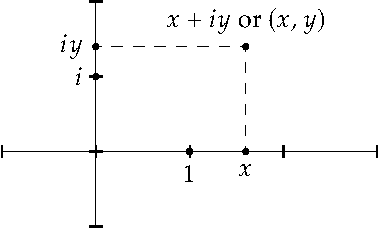
\includegraphics{figures/complexplane}
\caption{The points $1$, $i$, $x$, $iy$, and $x+iy$ in the complex
plane.\label{fig:complexplane}}
\end{myfigureht}

We generally use $x,y,r,s,t$ for real values and $z,w,\xi,\zeta$
for complex values, although that is not a hard and fast rule.  In
particular, $z$ is often used as a third real variable in $\R^3$.

\begin{defn}
Suppose $z= x+iy$.
We call $x$ 
the \emph{\myindex{real part}} of $z$, and 
we call $y$
the \emph{\myindex{imaginary part}} of $z$.  We write
\glsadd{not:realpart}\glsadd{not:imagpart}
\begin{equation*}
\Re\, z := x , \qquad
\Im\, z := y .
\end{equation*}
Define 
\glsadd{not:conj}
\emph{\myindex{complex conjugate}} as
\begin{equation*}
\bar{z} := x-iy ,
\end{equation*}
and define \emph{\myindex{modulus}} as
\glsadd{not:modulus}
\begin{equation*}
\sabs{z} := \sqrt{x^2+y^2} .
\end{equation*}
\end{defn}

Modulus is the complex analogue of the absolute value and
has similar properties.
For example,
$\sabs{zw} = \sabs{z} \, \sabs{w}$ (exercise).
The complex conjugate is a reflection of the plane across the real axis.
The real numbers are precisely those numbers for which the imaginary
part $y=0$.  In particular, they are precisely those numbers which satisfy
the equation
\begin{equation*}
z = \bar{z} .
\end{equation*}

As $\C$ is really $\R^2$, we let the metric on $\C$ be the standard
euclidean metric on $\R^2$.
In particular,
\begin{equation*}
\sabs{z} = d(z,0) , \qquad 
\text{and also} \qquad 
\sabs{z-w} = d(z,w) .
\end{equation*}
So the topology on $\C$ is
the same exact topology as the standard topology on $\R^2$
with the euclidean metric,
and $\sabs{z}$ is equal to the euclidean norm on $\R^2$.
Importantly, since $\R^2$ is a complete metric space, then
so is $\C$.
As $\sabs{z}$ is the euclidean norm on $\R^2$, we have the
\emph{triangle inequality}\index{triangle inequality!complex numbers}
of both flavors:
\begin{equation*}
\sabs{z+w} \leq \sabs{z}+\sabs{w} \qquad \text{and} \qquad
\big\lvert \sabs{z}-\sabs{w} \big\rvert \leq \sabs{z-w} .
\end{equation*}

The complex conjugate and the modulus are even more intimately related:
\begin{equation*}
\sabs{z}^2 =
x^2+y^2 =
(x+iy)(x-iy) =
z \bar{z} .
\end{equation*}

\begin{remark}
There is no natural ordering on the complex numbers.
In particular,
no ordering that makes the complex numbers into an ordered field.
Ordering is one of the things we lose when we go from real to complex
numbers.
\end{remark}

\subsection{Complex numbers and limits}

It is not hard to show that the algebraic operations are
continuous.  This is because convergence in 
$\R^2$ is the same as convergence for each component and we already know
that the real algebraic operations are continuous.  For example,
write $z_n = x_n + i\,y_n$ and
$w_n = s_n + i\,t_n$, and suppose that
$\lim \, z_n = z = x+i\,y$ and $\lim \, w_n = w = s+i\,t$.
Let us show
\begin{equation*}
\lim_{n\to\infty} z_n w_n = zw .
\end{equation*}
First,
\begin{equation*}
z_n w_n = (x_ns_n-y_nt_n) + i(x_nt_n+y_ns_n) .
\end{equation*}
The topology on $\C$ is the same as on $\R^2$, and so
$x_n \to x$, $y_n \to y$, $s_n \to s$, and $t_n \to t$.
Hence,
\begin{equation*}
\lim_{n\to\infty} (x_ns_n-y_nt_n) = xs-yt \qquad \text{and} \qquad
\lim_{n\to\infty} (x_nt_n+y_ns_n) = xt+ys .
\end{equation*}
As
$(xs-yt)+i(xt+ys) = zw$, then
\begin{equation*}
\lim_{n\to\infty} z_n w_n = zw .
\end{equation*}

Similarly the modulus and the complex conjugate are continuous functions.  We
leave the proof of the following proposition as an exercise.

\begin{prop} \label{prop:continuityofcomplex}
Suppose $\{ z_n \}$, $\{ w_n \}$ are sequences of complex numbers converging
to $z$ and $w$ respectively.  Then
\begin{enumerate}[(i)]
\item
$\displaystyle \lim_{n\to \infty} z_n + w_n = z + w$.
\item
$\displaystyle \lim_{n\to \infty} z_n w_n = z w$.
\item
Assuming $w_n \not= 0$ for all $n$ and $w\not= 0$,
$\displaystyle \lim_{n\to \infty} \frac{z_n}{w_n} = \frac{z}{w}$.
\item
$\displaystyle \lim_{n\to \infty} \sabs{z_n} = \sabs{z}$.
\item
$\displaystyle \lim_{n\to \infty} \bar{z}_n = \bar{z}$.
\end{enumerate}
\end{prop}

As we have seen above, convergence in $\C$ is the same as convergence in
$\R^2$.  In particular, a sequence in $\C$ converges if and only if
the real and imaginary parts converge.  Therefore, feel free to apply
everything you have learned about convergence in $\R^2$, as well as
applying results about real numbers to the real and imaginary parts.

We also need convergence of complex series.  Let $\{ z_n \}$ be a
sequence of complex
numbers. The series
\begin{equation*}
\sum_{n=1}^\infty z_n
\end{equation*}
\emph{converges}\index{converges!complex series} if the limit of partial sums converges, that is, if
\begin{equation*}
\lim_{k\to\infty} \sum_{n=1}^k z_n \qquad \text{exists.}
\end{equation*}
As before, we sometimes write $\sum z_n$ for the series.
A series \emph{converges absolutely}\index{converges
absolutely!complex series} if $\sum \sabs{z_n}$ converges.

We say a series
is \emph{Cauchy}\index{Cauchy!complex series}
if the sequence of partial sums is Cauchy.  The following two
propositions have essentially the same proofs as for real series and we
leave them as exercises.

\begin{prop} \label{prop:cachysercomplex}
The complex series $\sum z_n$ is Cauchy if for every $\epsilon > 0$, 
there exists an $M \in \N$ such that for every $n \geq M$
and every $k > n$, we have
\begin{equation*}
\abs{ \sum_{j={n+1}}^k z_j }
< \epsilon .
\end{equation*}
\end{prop}

\begin{prop} \label{prop:absconvmeansconv}
If a complex series $\sum z_n$ converges absolutely, then it converges.
\end{prop}

The series $\sum \sabs{z_n}$ is a real series.  All the
convergence tests (ratio test, root test, etc.)\ that talk about
absolute convergence work with the numbers $\sabs{z_n}$, that is, they
are really talking about convergence of series of nonnegative real
numbers.
You
can directly apply these tests
them without needing to reprove anything for complex
series.

\subsection{Complex-valued functions}

When we deal with complex-valued functions
$f \colon X \to \C$, what we often do is to write
$f = u+i\,v$ for real-valued functions $u \colon X \to \R$ and $v \colon X \to
\R$.

Suppose we wish to integrate
$f \colon [a,b] \to \C$.  We write
$f = u+i\,v$ for real-valued $u$ and $v$.
We say that $f$ is \emph{Riemann integrable}\index{Riemann
integrable!complex-valued function}
if $u$ and $v$ are Riemann
integrable, and in this case we define
\begin{equation*}
\int_a^b f := \int_a^b u + i \int_a^b v .
\end{equation*}
We make the same definition for every other type of integral (improper,
multivariable, etc.).

Similarly when we differentiate, write $f \colon [a,b] \to \C$ as
$f = u+i\,v$.  Thinking of $\C$ as $\R^2$ we say that $f$ is differentiable
if $u$ and $v$ are differentiable.  For a function valued in $\R^2$, the derivative
was represented by a vector in $\R^2$.  Now a vector in $\R^2$ is a complex
number.  In other words,
we write
the
\emph{derivative}\index{derivative!complex-valued function}
as
\glsadd{not:mvder}
\begin{equation*}
f'(t) := u'(t) + i \, v'(t) .
\end{equation*}
The linear operator representing the derivative is the multiplication by
the complex number $f'(t)$, so nothing is lost in this identification.


\subsection{Exercises}

\begin{exercise}
Check that $\C$ is a field.
\end{exercise}

\begin{exercise}
Prove that for $z,w \in \C$, we have
$\sabs{zw} = \sabs{z} \, \sabs{w}$.
\end{exercise}

\begin{exercise}
Finish the proof of \propref{prop:continuityofcomplex}.
\end{exercise}

\begin{exercise}
Prove \propref{prop:cachysercomplex}.
\end{exercise}

\begin{exercise}
Prove \propref{prop:absconvmeansconv}.
\end{exercise}

\begin{samepage}
\begin{exercise}
Considering the definition of complex multiplication, given $x +iy$
define the matrix
$\left[ \begin{smallmatrix} x & -y \\ y & x \end{smallmatrix} \right]$.
Prove that
\begin{enumerate}[a)]
\item
The action of this matrix on a vector $(s,t)$ is the same
as the action of multiplying $(x+iy)(s+it)$.
\item
Multiplying two such matrices is the same multiplying the underlying complex
numbers and then finding the corresponding matrix for the product.
In other words, we can think of the field $\C$ as also a subset of
the 2-by-2 matrices.
\item
Show that 
$\left[ \begin{smallmatrix} x & -y \\ y & x \end{smallmatrix} \right]$
has eigenvalues $x+iy$ and $x-iy$.  Recall that $\lambda$ is
an eigenvalue of a matrix $A$ if $A-\lambda I$ (a complex matrix in our case)
is not invertible, or in other words
if it has linearly dependent rows: That is, one row is a (complex) multiple
of the other
\end{enumerate}
\end{exercise}
\end{samepage}

\begin{exercise}
Prove the Bolzano--Weierstrass theorem for complex sequences.
Suppose $\{ z_n \}$ is a bounded sequence of complex numbers, that
is, there exists an $M$ such that $\sabs{z_n} \leq M$ for all $n$.  Prove
that there exists a subsequence $\{ z_{n_k} \}$ that converges to some $z
\in \C$.
\end{exercise}

\begin{exercise}
\leavevmode
\begin{enumerate}[a)]
\item
Prove that there is no simple mean value theorem for complex-valued
functions:  Find a differentiable function $f \colon [0,1] \to \C$ such that
$f(0) = f(1) = 0$, but $f'(t) \not= 0$ for all $t \in [0,1]$.
\item
However, there is a weaker form of the mean value theorem as there is for vector-valued
functions.  Prove: If $f \colon [a,b] \to \C$ is continuous and differentiable in
$(a,b)$, and for some $M$, $\sabs{f'(x)} \leq M$ for all $x \in (a,b)$, then
$\sabs{f(b)-f(a)} \leq M \sabs{b-a}$.
\end{enumerate}
\end{exercise}

\begin{exercise}
Prove that there is no simple mean value theorem for integrals
for complex-valued
functions:  Find a continuous function $f \colon [0,1] \to \C$ such that
$\int_0^1 f = 0$ but $f(t) \not= 0$ for all $t \in [0,1]$.
\end{exercise}


%%%%%%%%%%%%%%%%%%%%%%%%%%%%%%%%%%%%%%%%%%%%%%%%%%%%%%%%%%%%%%%%%%%%%%%%%%%%%%

\sectionnewpage
\section{Swapping limits}
\label{sec:swaplim}

\sectionnotes{2 lectures}

\subsection{Continuity}

Let us get back to swapping limits and expand on
\volIref{\chapterref*{vI-fs:chapter} of volume I}{\chapterref{fs:chapter}}.
Let $\{ f_n \}$ be a sequence
of functions $f_n \colon X \to Y$ for a set $X$ and a metric space $Y$.
Let $f \colon X \to Y$ be a
function and for every $x \in X$ suppose that
\begin{equation*}
f(x) = \lim_{n\to \infty} f_n(x) .
\end{equation*}
We say the sequence $\{ f_n \}$
\emph{\myindex{converges pointwise}}\index{pointwise convergence} to $f$.

For $Y=\C$, a series
\emph{converges pointwise}\index{converges pointwise!complex series}\index{pointwise convergence!complex series} if
for every $x \in X$, we have
\begin{equation*}
f(x) = \lim_{n\to \infty} \sum_{k=1}^n f_k(x) =
\sum_{k=1}^\infty f_k(x) .
\end{equation*}

\medskip

The question is:
If $f_n$ are all continuous, is $f$ continuous?  Differentiable?
Integrable?  What are the derivatives or integrals of $f$?

For example, for continuity of the pointwise limit of a sequence $\{ f_n
\}$, we are asking if
\begin{equation*}
\lim_{x\to x_0} \lim_{n\to\infty} f_n(x)
\overset{?}{=}
\lim_{n\to\infty} \lim_{x\to x_0} f_n(x) .
\end{equation*}
We don't even a priory know if both sides exist, let alone if they are equal each other.

\begin{example}
The functions $f_n \colon \R \to \R$,
\begin{equation*}
f_n(x) := \frac{1}{1+nx^2},
\end{equation*}
are continuous and converge pointwise to the discontinuous function
\begin{equation*}
f(x) := 
\begin{cases}
1 & \text{if } x=0, \\
0 & \text{else.}
\end{cases}
\end{equation*}
\end{example}

So pointwise convergence is not enough to preserve continuity (nor even
boundedness).  For that, we need uniform convergence.

Let $f_n \colon X \to Y$ be functions.  Then
$\{f_n\}$ \emph{\myindex{converges uniformly}}\index{uniform convergence}
to $f$ if
for every $\epsilon > 0$, there exists an $M$ such that
for all $n \geq M$ and all $x \in X$, we have
\begin{equation*}
d\bigl(f_n(x),f(x)\bigr) < \epsilon .
\end{equation*}

A series $\sum f_n$ of complex-valued functions converges uniformly if the sequence of
partial sums converges uniformly, that is for every $\epsilon > 0$
there exists an $M$ such that
for all $n \geq M$ and all $x \in X$
\begin{equation*}
\abs{\left(\sum_{k=1}^n f_k(x)\right)-f(x)} < \epsilon .
\end{equation*}

The simplest property preserved by uniform convergence is
boundedness.  We leave the proof of the following proposition as an
exercise.  It is almost identical to the proof for real-valued functions.

\begin{prop} \label{prop:uniformconvbounded}
Let $X$ be a set and $(Y,d)$ a metric space.
If $f_n \colon X \to Y$ are bounded functions and converge uniformly to $f
\colon X \to Y$, then $f$ is bounded.
\end{prop}

If $X$ is a set and $(Y,d)$ is a metric space, then a sequence $f_n \colon X
\to Y$ is \emph{\myindex{uniformly Cauchy}} if for every $\epsilon > 0$, there is an $M$ such that
for all $n, m \geq M$ and all $x \in X$, we have
\begin{equation*}
d\bigl(f_n(x),f_m(x)\bigr) < \epsilon .
\end{equation*}
The notion is the same as for real-valued functions.
The proof of the following proposition is
again essentially the same as in that setting and
is left as an exercise.

\begin{prop} \label{prop:unifcauchymetric}
Let $X$ be a set, $(Y,d)$ be a metric space, and
$f_n \colon X \to Y$ be functions.
If $\{ f_n \}$ converges uniformly,
then $\{f_n\}$ is uniformly Cauchy.  Conversely, if 
$\{f_n\}$ is uniformly Cauchy and $(Y,d)$ is Cauchy-complete,
then $\{f_n\}$ converges uniformly.
\end{prop}

For $f \colon X \to \C$, we write\glsadd{not:uniformnorm}
\begin{equation*}
\snorm{f}_u := \sup_{x \in X} \sabs{f(x)} .
\end{equation*}
We call $\snorm{\cdot}_u$
the \emph{\myindex{supremum norm}} or \emph{\myindex{uniform norm}}.
Then a sequence of functions
$f_n \colon X \to \C$ converges uniformly to $f \colon X \to \C$ if and only if
\begin{equation*}
\lim_{n\to \infty} \snorm{f_n-f}_u = 0 .
\end{equation*}

The supremum norm satisfies the triangle inequality: For every $x \in X$,
\begin{equation*}
\sabs{f(x)+g(x)} \leq
\sabs{f(x)}+\sabs{g(x)} \leq
\snorm{f}_u+\snorm{g}_u .
\end{equation*}
Take a supremum on the left to get
\begin{equation*}
\snorm{f+g}_u \leq
\snorm{f}_u+\snorm{g}_u .
\end{equation*}

For a compact metric space $X$,
the uniform norm is a norm on the vector space $C(X,\C)$.
We leave it as an exercise.
While we will not need it, $C(X,\C)$ is in fact a complex
vector space, that is, in the definition of a vector space we can replace
$\R$ with $\C$.
Convergence in the metric space $C(X,\C)$ is
uniform convergence.

We will study a couple of types of series of functions, and
a useful test for uniform convergence of a series is the 
so-called \emph{\myindex{Weierstrass $M$-test}}.

\begin{thm}[\myindex{Weierstrass $M$-test}] \label{thm:weiermtest}
Let $X$ be a set.
Suppose $f_n \colon X \to \C$ are functions and $M_n > 0$ numbers such
that
\begin{equation*}
\sabs{f_n(x)}\leq M_n \quad \text{for all } x \in X,
\qquad \text{and} \qquad
\sum_{n=1}^\infty M_n
\quad \text{converges}.
\end{equation*}
Then
\begin{equation*}
\sum_{n=1}^\infty f_n(x)
\quad \text{converges uniformly}.
\end{equation*}
\end{thm}

Another way to state the theorem is to say that if
$\sum \snorm{f_n}_u$ converges, then $\sum f_n$ converges uniformly.
Note that the converse of this theorem is not true.
Also note that applying the theorem to $\sum \sabs{f_n(x)}$ gives that
a series satisfying the $M$-test also converges uniformly, so the series converges both absolutely
and uniformly.

\begin{proof}
Suppose $\sum M_n$ converges.  Given $\epsilon > 0$,
we have that the partial sums of $\sum M_n$ are Cauchy so
there is an $N$ such that for all $m, n \geq N$ with $m \geq n$, we have
\begin{equation*}
\sum_{k=n+1}^m M_k < \epsilon .
\end{equation*}
We estimate a Cauchy difference of the partial
sums of the functions
\begin{equation*}
\abs{\sum_{k=n+1}^m f_k(x)} \leq
\sum_{k=n+1}^m \sabs{f_k(x)} \leq
\sum_{k=n+1}^m M_k < \epsilon .
\end{equation*}
We are done by \propref{prop:cachysercomplex}.
\end{proof}

\begin{example} \label{example:sinnsqfourier}
The series
\begin{equation*}
\sum_{n=1}^\infty \frac{\sin(nx)}{n^2}
\end{equation*}
converges uniformly on $\R$.  See \figureref{fig:fouriersern2}.
This is a Fourier series,
we will see more of these in a later section.  Proof:
The series converges uniformly because
$\sum_{n=1}^\infty \frac{1}{n^2}$
converges and
\begin{equation*}
\abs{\frac{\sin(nx)}{n^2}} \leq 
\frac{1}{n^2} .
\end{equation*}
\end{example}

\begin{myfigureht}
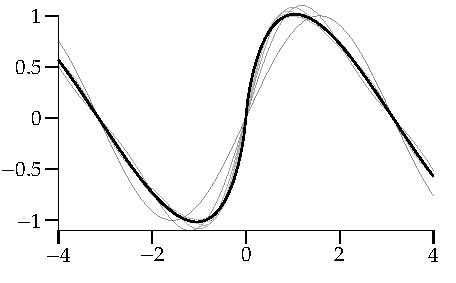
\includegraphics{figures/fouriersern2}
\caption{Plot of 
$\sum_{n=1}^\infty \frac{\sin(n x)}{n^2}$ including
the first 8 partial sums in various shades of gray.\label{fig:fouriersern2}}
\end{myfigureht}

\begin{example}
The series
\begin{equation*}
\sum_{n=0}^\infty \frac{x^n}{n!} 
\end{equation*}
converges uniformly on every bounded interval.
This series is a power series that we will study shortly.
Proof: Take the interval $[-r,r] \subset \R$ (every bounded interval
is contained in some $[-r,r]$).
The series $\sum_{n=0}^\infty \frac{r^n}{n!}$ converges by the ratio test,
so $\sum_{n=0}^\infty \frac{x^n}{n!}$ converges uniformly on $[-r,r]$ as
\begin{equation*}
\abs{\frac{x^n}{n!} } \leq 
\frac{r^n}{n!} .
\end{equation*}
\end{example}

Now we would love to say something about the limit.  For example, is it
continuous?


\begin{prop} \label{prop:uniformswitch}
Let $(X,d_X)$ and $(Y,d_Y)$ be metric spaces.
Suppose $f_n \colon X \to Y$ converge uniformly to
 $f \colon X \to Y$.  
Let $\{ x_k \}$ be a sequence in $X$ and $x := \lim \, x_k$.  Suppose
that
\begin{equation*}
a_n := \lim_{k \to \infty} f_n(x_k)
\end{equation*}
exists for all $n$.  Then
$\{a_n\}$ converges and 
\begin{equation*}
\lim_{k \to \infty} f(x_k) = \lim_{n\to\infty} a_n .
\end{equation*}
\end{prop}

In other words,
\begin{equation*}
\lim_{k \to \infty} \lim_{n\to\infty} f_n(x_k) =
\lim_{n \to \infty} \lim_{k\to\infty} f_n(x_k) .
\end{equation*}

\begin{proof}
First we show that $\{ a_n \}$ converges.  As
$\{ f_n \}$ converges uniformly it is uniformly Cauchy. 
Let $\epsilon > 0$ be given.  There is
an $M$ such that for all $m,n \geq M$, we have
\begin{equation*}
d_Y\bigl(f_n(x_k),f_m(x_k)\bigr) < \epsilon \qquad \text{for all } k .
\end{equation*}
Note that
$d_Y(a_n,a_m) \leq
d_Y\bigl(a_n,f_n(x_k)\bigr) +
d_Y\bigl(f_n(x_k),f_m(x_k)\bigr) +
d_Y\bigl(f_m(x_k),a_m\bigr)$ and take the limit as $k \to \infty$ to find
\begin{equation*}
d_Y(a_n,a_m) \leq \epsilon .
\end{equation*}
Hence $\{a_n\}$ is Cauchy and converges since $Y$ is complete.  Write
$a := \lim \, a_n$.

Find a $k \in \N$ such that
\begin{equation*}
d_Y\bigl(f_k(p),f(p)\bigr) < \nicefrac{\epsilon}{3}
\end{equation*}
for all $p \in X$.  Assume $k$ is large enough
so that
\begin{equation*}
d_Y(a_k,a) < \nicefrac{\epsilon}{3}  .
\end{equation*}
Find an $N \in \N$ such that for $m \geq N$,
\begin{equation*}
d_Y\bigl(f_k(x_m),a_k\bigr) < \nicefrac{\epsilon}{3}  .
\end{equation*}
Then for
$m \geq N$,
\begin{equation*}
d_Y\bigl(f(x_m),a\bigr)
\leq
d_Y\bigl(f(x_m),f_k(x_m)\bigr)
+
d_Y\bigl(f_k(x_m),a_k\bigr)
+
d_Y\bigl(a_k,a\bigr)
<
\nicefrac{\epsilon}{3} +
\nicefrac{\epsilon}{3} +
\nicefrac{\epsilon}{3} = \epsilon . \qedhere
\end{equation*}
\end{proof}

We obtain an immediate corollary about continuity.

\begin{cor} \label{cor:metricuniformcontinuous}
Let $X$ and $Y$ be metric spaces.
If $f_n \colon X \to Y$ are continuous functions
such that
$\{ f_n \}$ converges uniformly to $f \colon X \to Y$,
then $f$ is continuous.
\end{cor}

The converse is not true.  Just because the limit is continuous doesn't mean
that the convergence is uniform.  For example:
$f_n \colon (0,1) \to \R$ defined by $f_n(x) := x^n$ converge to
the zero function, but not uniformly.  However, if we add extra conditions
on the sequence, we can obtain a partial converse such as Dini's theorem,
\volIref{see \exerciseref*{vI-exercise:dinisthm} from volume I}{see \exerciseref{exercise:dinisthm}}.

In \exerciseref{exercise:CXCnormedspace} the reader is asked to prove
that for a compact $X$, $C(X,\C)$ is a normed vector space
with the uniform norm, and hence a metric space.  We have just shown that
$C(X,\C)$ is Cauchy-complete:  \propref{prop:unifcauchymetric} says that a Cauchy
sequence in $C(X,\C)$ converges uniformly to some function,
and \corref{cor:metricuniformcontinuous} shows that the limit is
continuous and hence in $C(X,\C)$.

\begin{cor}
Let $(X,d)$ be a compact metric space.
Then $C(X,\C)$ is a Cauchy-complete metric space.
\end{cor}

\begin{example}
By \exampleref{example:sinnsqfourier}
the Fourier series 
\begin{equation*}
\sum_{n=1}^\infty \frac{\sin(nx)}{n^2}
\end{equation*}
converges uniformly and hence is continuous by \corref{cor:metricuniformcontinuous} (as is visible
in \figureref{fig:fouriersern2}).
\end{example}

\subsection{Integration}

\begin{prop} \label{prop:complexlimitswapintegral}
Suppose $f_n \colon [a,b] \to \C$
are Riemann integrable and suppose that $\{ f_n \}$ converges
uniformly to $f \colon [a,b] \to \C$.  Then $f$ is Riemann integrable
and
\begin{equation*}
\int_a^b f = \lim_{n\to \infty} \int_a^b f_n .
\end{equation*}
\end{prop}

Since the integral of a complex-valued function is just the integral of
the real and imaginary parts separately,
the proof follows directly by the results of
\volIref{\chapterref*{vI-fs:chapter} of volume I}{\chapterref{fs:chapter}}.
We leave the details as an exercise.

\begin{cor}
Suppose $f_n \colon [a,b] \to \C$
are Riemann integrable and suppose that
\begin{equation*}
\sum_{n=1}^\infty f_n(x)
\end{equation*}
converges uniformly.  Then the series is Riemann integrable on $[a,b]$
and
\begin{equation*}
\int_a^b \sum_{n=1}^\infty f_n(x) \,dx
=
\sum_{n=1}^\infty \int_a^b f_n(x) \,dx
\end{equation*}
\end{cor}

\begin{example}
Let us show how to integrate a Fourier series.
\begin{equation*}
\int_{0}^x \sum_{n=1}^\infty \frac{\cos(nt)}{n^2} \,dt
=
\sum_{n=1}^\infty \int_{0}^x \frac{\cos(nt)}{n^2}\,dt
=
\sum_{n=1}^\infty \frac{\sin(nx)}{n^3}
\end{equation*}
The swapping of integral and sum is possible because of uniform convergence,
which we have proved before using the Weierstrass $M$-test
(\thmref{thm:weiermtest}).
\end{example}

We remark that we can swap integrals and limits under far less stringent hypotheses,
but for that we would need a stronger integral than the Riemann integral.
E.g.\ the Lebesgue integral.

\subsection{Differentiation}

Recall that a complex-valued function
$f \colon [a,b] \to \C$, where $f(x) = u(x)+i\,v(x)$,
is differentiable, if $u$ and $v$ are differentiable
and the derivative is
\begin{equation*}
f'(x) = u'(x)+i\,v'(x) .
\end{equation*}

The proof of the following theorem is to apply the corresponding theorem for
real functions to $u$ and $v$, and is left as an exercise.

\begin{thm} \label{thm:dersconvergecomplex}
Let $I \subset \R$ be a bounded interval and let
$f_n \colon I \to \C$ be continuously differentiable functions.
Suppose $\{ f_n' \}$ converges uniformly to $g \colon I \to \C$,
and suppose $\{ f_n(c) \}_{n=1}^\infty$ is a
convergent sequence for some $c \in I$.  Then $\{ f_n \}$ converges uniformly to 
a continuously differentiable function $f \colon I \to \C$, and $f' = g$.
\end{thm}

Uniform limits of the functions themselves are not enough, and can make
matters even worse.  In \sectionref{sec:stoneweier} we will prove that
continuous functions are uniform limits of polynomials, yet as the following
example demonstrates, a continuous function need not be differentiable
anywhere.

\begin{example}
There exist continuous nowhere differentiable functions.
Such functions are often called
\emph{Weierstrass functions}\index{Weierstrass function},
although this
particular one, essentially due to
Takagi\footnote{\href{https://en.wikipedia.org/wiki/Teiji_Takagi}{Teiji
Takagi} (1875--1960) was a Japanese mathematician.}, is a different example than what Weierstrass gave.

Define
\begin{equation*}
\varphi(x) :=\sabs{x} \qquad \text{for } x \in [-1,1] .
\end{equation*}
Extend the definition of $\varphi$ to all of $\R$ by making it
2-periodic:
Decree that
$\varphi(x) = \varphi(x+2)$.  The function $\varphi \colon \R \to \R$
is continuous, in fact $\sabs{\varphi(x)-\varphi(y)} \leq \sabs{x-y}$ (why?).
See \figureref{fig:triangwave}.
\begin{myfigureht}
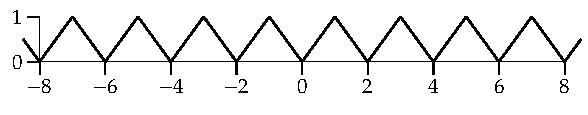
\includegraphics{figures/triangwave}
\caption{The 2-periodic function $\varphi$.\label{fig:triangwave}}
\end{myfigureht}

As $\sum {\left(\frac{3}{4}\right)}^n$ converges and $\sabs{\varphi(x)} \leq
1$ for all $x$, we have by the $M$-test
(\thmref{thm:weiermtest}) that
\begin{equation*}
f(x) := \sum_{n=0}^\infty 
{\left(\frac{3}{4}\right)}^n \varphi(4^n x)
\end{equation*}
converges uniformly and hence is continuous.
See \figureref{fig:nowherediff}.

\begin{myfigureht}
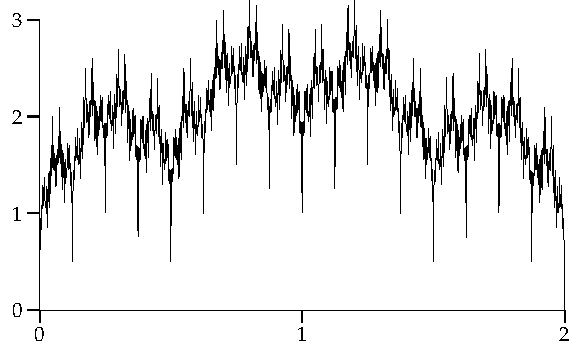
\includegraphics{figures/nowherediff}
\caption{Plot of the nowhere differentiable function $f$.\label{fig:nowherediff}}
\end{myfigureht}

We claim $f \colon
\R \to \R$ is nowhere differentiable.
Fix $x$, and we will show $f$ is not differentiable at $x$.
Define
\begin{equation*}
\delta_m := \pm \frac{1}{2} 4^{-m} ,
\end{equation*}
where the sign is chosen so that there is no integer
between $4^m x$ and $4^m(x+\delta_m) = 4^m x \pm \frac{1}{2}$.

We want to look at the difference quotient
\begin{equation*}
\frac{f(x+\delta_m)-f(x)}{\delta_m}
=
\sum_{n=0}^\infty 
{\left(\frac{3}{4}\right)}^n
\frac{\varphi\bigl(4^n(x+\delta_m)\bigr)-\varphi(4^nx)}{\delta_m} .
\end{equation*}
Fix $m$ for a moment.  Consider the expression inside the series:
\begin{equation*}
\gamma_{n} :=
\frac{\varphi\bigl(4^n(x+\delta_m)\bigr)-\varphi(4^nx)}{\delta_m} .
\end{equation*}
If $n > m$, then $4^n\delta_m$ is an even integer.  As $\varphi$
is 2-periodic we get that $\gamma_n = 0$.

As there is no integer between 
$4^m(x+\delta_m) = 4^m x\pm\nicefrac{1}{2}$ and $4^m x$, then on this interval
$\varphi(t) = \pm t + \ell$ for some integer $\ell$.
In particular,
$\abs{\varphi\bigl(4^m(x+ \delta_m)\bigr)-\varphi(4^mx)} =
\abs{4^mx\pm\nicefrac{1}{2}-4^mx} = \nicefrac{1}{2}$.  Therefore,
\begin{equation*}
\sabs{\gamma_m} =
\abs{
\frac{\varphi\bigl(4^m(x+\delta_m)\bigr)-\varphi(4^mx)}{\pm (\nicefrac{1}{2}) 4^{-m}}
}
= 4^m .
\end{equation*}
Similarly, suppose $n < m$.  Since $\sabs{\varphi(s) -\varphi(t)} \leq
\sabs{s-t}$,
\begin{equation*}
\sabs{\gamma_n} =
\abs{\frac{\varphi\bigl(4^nx\pm(\nicefrac{1}{2})4^{n-m}\bigr)-\varphi(4^nx)}{\pm
(\nicefrac{1}{2}) 4^{-m}}}
\leq
\abs{\frac{\pm(\nicefrac{1}{2})4^{n-m}}{\pm (\nicefrac{1}{2}) 4^{-m}}} = 4^n
.
\end{equation*}

And so
\begin{equation*}
\begin{split}
\abs{
\frac{f(x+\delta_m)-f(x)}{\delta_m}
}
%& =
%\abs{
%\sum_{n=0}^\infty 
%{\left(\frac{3}{4}\right)}^n
%\frac{\varphi\bigl(4^n(x+\delta_m)\bigr)-\varphi(4^nx)}{\delta_m}
%}
=
\abs{
\sum_{n=0}^\infty 
{\left(\frac{3}{4}\right)}^n
\gamma_n
}
& =
\abs{
\sum_{n=0}^m 
{\left(\frac{3}{4}\right)}^n
\gamma_n
}
\\
& \geq
\abs{
{\left(\frac{3}{4}\right)}^m
\gamma_m}
-
\abs{
\sum_{n=0}^{m-1} 
{\left(\frac{3}{4}\right)}^n
\gamma_n
}
\\
& \geq
3^m
-
\sum_{n=0}^{m-1} 
3^n
=
3^m
-
\frac{3^{m}-1}{3-1}
=
\frac{3^m +1}{2} .
\end{split}
\end{equation*}
As $m \to \infty$, we have
$\delta_m \to 0$, but $\frac{3^m+1}{2}$
goes to infinity.  Hence $f$ cannot be differentiable at $x$.
\end{example}

\subsection{Exercises}

\begin{exercise}
Prove \propref{prop:uniformconvbounded}.
\end{exercise}

\begin{exercise}
Prove \propref{prop:unifcauchymetric}.
\end{exercise}

\begin{exercise} \label{exercise:CXCnormedspace}
Suppose $(X,d)$ is a compact metric space.
Prove that $\snorm{\cdot}_u$ is a norm on the vector space of
continuous complex-valued functions $C(X,\C)$.
\end{exercise}

\begin{exercise}
\leavevmode
\begin{enumerate}[a)]
\item
Prove that
$f_n(x) := 2^{-n} \sin(2^n x)$
converge uniformly to zero, but there exists a dense set $D \subset \R$
such that $\lim_{n\to\infty} f_n'(x) = 1$ for all $x \in D$.
\item
Prove that
$\sum_{n=1}^\infty 2^{-n} \sin(2^n x)$
converges uniformly to a continuous function,
and there exists a dense set $D \subset \R$
where the derivatives of the partial sums do not converge.
\end{enumerate}
\end{exercise}

\begin{exercise}
Suppose $(X,d)$ is a compact metric space.
Prove that $\snorm{f}_{C^1} := \snorm{f}_u+\snorm{f'}_u$
is a norm on the vector space of
continuously differentiable complex-valued functions $C^1(X,\C)$.
\end{exercise}

\begin{exercise}
Prove \thmref{thm:dersconvergecomplex}.
\end{exercise}

\begin{exercise}
Prove \propref{prop:complexlimitswapintegral} by reducing to the real
result.
\end{exercise}

\begin{exercise}
Work through the following counterexample to the converse of
the Weierstrass $M$-test (\thmref{thm:weiermtest}).  Define
$f_n \colon [0,1] \to \R$ by
\begin{equation*}
f_n(x) :=
\begin{cases}
\frac{1}{n} & \text{if } \frac{1}{n+1} < x < \frac{1}{n},\\
0	    & \text{else.}
\end{cases}
\end{equation*}
Prove that $\sum f_n$ converges uniformly, but $\sum \snorm{f_n}_u$
does not.
\end{exercise}

\begin{exercise}
Suppose $f_n \colon [0,1] \to \R$ are monotone increasing functions and
suppose that $\sum f_n$ converges pointwise.  Prove that $\sum f_n$
converges uniformly.
\end{exercise}

\begin{exercise}
Prove that
\begin{equation*}
\sum_{n=1}^\infty e^{-nx}
\end{equation*}
converges for all $x > 0$ to a differentiable function.
\end{exercise}

%%%%%%%%%%%%%%%%%%%%%%%%%%%%%%%%%%%%%%%%%%%%%%%%%%%%%%%%%%%%%%%%%%%%%%%%%%%%%%

\sectionnewpage
\section{Power series and analytic functions}
\label{sec:analfuncs}

\sectionnotes{2--3 lectures}

\subsection{Analytic functions}

A (complex) power series is a series of the form
\begin{equation*}
\sum_{n=0}^\infty c_n {(z-a)}^n
\end{equation*}
for $c_n, z, a \in \C$.  We say the series
\emph{converges}\index{converges!power series} if the series converges for
some $z \not= a$.

Let $U \subset \C$ be an open set and
$f \colon U \to \C$ a function.
Suppose that for every $a \in U$ there exists a $\rho > 0$ and a power
series convergent to the function
\begin{equation*}
f(z) = \sum_{n=0}^\infty c_n {(z-a)}^n
\end{equation*}
for all $z \in B(a,\rho)$.
Then we say $f$ is an \emph{\myindex{analytic}} function.

Similarly if we have an interval $(a,b) \subset \R$, we say that $f \colon (a,b)
\to \C$ is analytic or perhaps \emph{\myindex{real-analytic}}
if for each point $c \in
(a,b)$ there is a power series around $c$ that converges in some
$(c-\rho,c+\rho)$
for some $\rho > 0$.

As we will sometimes talk about real and sometimes about complex power
series we will use $z$ to denote a complex number and $x$ a real number, but
we will always mention which case we are working with.

An analytic function has different expansions around different
points.  Also the convergence does not automatically happen on the entire
domain of the function.  For example, if $\sabs{z} < 1$, then
\begin{equation*}
\frac{1}{1-z} = \sum_{n=0}^\infty z^n .
\end{equation*}
While the left-hand side exists on all of $z \not= 1$, the right-hand side
happens to converge only if $\sabs{z} < 1$.  See a graph
of a small piece of $\frac{1}{1-z}$ in \figureref{fig:1over1mz}.
Notice that we can't graph the
function itself, we can only graph its real or imaginary parts for lack
of dimensions in our universe.

\begin{myfigureht}
\subimport*{figures/}{real_imag_1over1mz.pdf_t}
\caption{Graphs of the real and imaginary parts of $z=x+iy \mapsto \frac{1}{1-z}$
in the square $[-0.8,0.8]^2$.  The singularity at $z=1$ is marked with a
vertical dashed line.\label{fig:1over1mz}}
\end{myfigureht}

\subsection{Convergence of power series}

We proved several results for power series of a real variable in
\volIref{\sectionref*{vI-sec:moreonseries} of volume I}{\sectionref{sec:moreonseries}}.   For the most part the convergence
properties of power series deal with the series
$\sum \sabs{c_k} \, \sabs{z-a}^k$ and so we have already proved many results about complex power
series.  In particular, we computed the so-called
\emph{radius of convergence} of a power series.

\begin{samepage}
\begin{prop}
Let $\sum_{n=0}^\infty c_n {(z-a)}^n$ be a power series.
There exists a $\rho \in [0,\infty]$ such that
\begin{enumerate}[(i)]
\item If $\rho = 0$, then the series diverges.
\item If $\rho = \infty$, then the series converges for all $z \in \C$.
\item If $0 < \rho < \infty$, then the
series converges absolutely on $B(a,\rho)$,
and diverges when $\sabs{z-a} > \rho$.
\end{enumerate}
Furthermore, if $0 < r < \rho$, then
the series converges uniformly on the closed ball $C(a,r)$.
\end{prop}
\end{samepage}

\begin{proof}
We use the real version of this proposition,
\volIref{\propref*{vI-prop:powerserrealradius} in volume I}{\propref{prop:powerserrealradius}}.
Let
\begin{equation*}
R := \limsup_{n\to\infty} \sqrt[n]{\sabs{c_n}} .
\end{equation*}
If $R = 0$, then
$\sum_{n=0}^\infty \sabs{c_n} \, \sabs{z-a}^n$ converges for all $z$.
If $R = \infty$, then
$\sum_{n=0}^\infty \sabs{c_n} \, \sabs{z-a}^n$ converges only at $z=a$.
Otherwise, let $\rho := \nicefrac{1}{R}$ and
$\sum_{n=0}^\infty \sabs{c_n} \, \sabs{z-a}^n$ converges when
$\sabs{z-a} < \rho$, and diverges (in fact the terms of the series
do not go to zero) when $\sabs{z-a} > \rho$.

To prove the furthermore suppose
$0 < r < \rho$ and $z \in C(a,r)$.  Then
consider the partial sums
\begin{equation*}
\abs{\sum_{n=0}^k c_n {(z-a)}^n}
\leq
\sum_{n=0}^k \sabs{c_n} \sabs{z-a}^n
\leq
\sum_{n=0}^k \sabs{c_n} r^n . \qedhere
\end{equation*}
\end{proof}

The number $\rho$ is called the \emph{\myindex{radius of convergence}}.
See \figureref{fig:radiusconvcomplex}.
The radius of convergence gives us a disk around $a$ where the series converges.  A power series
is convergent if $\rho > 0$.
\begin{myfigureht}
\subimport*{figures/}{radiusconvcomplex.pdf_t}
\caption{Radius of convergence.\label{fig:radiusconvcomplex}}
\end{myfigureht}

If $\sum c_n {(z-a)}^n$ converges for some $z$, then
\begin{equation*}
\sum c_n {(w-a)}^n
\end{equation*}
converges absolutely whenever $\sabs{w-a} < \sabs{z-a}$.
Conversely if the series diverges at $z$, then it must diverge at $w$
whenever $\sabs{w-a} > \sabs{z-a}$.
This means that to show
that the radius of convergence is at least some number, we simply need to
show convergence at some point by any method we know.

\begin{example}
Let us list some series we already know:
\begin{align*}
& &
& \sum_{n=0}^\infty z^n
& & \text{has radius of convergence } 1.
& &
\\
& &
& \sum_{n=0}^\infty \frac{1}{n!} z^n
& & \text{has radius of convergence } \infty.
& &
\\
& &
& \sum_{n=0}^\infty n^n z^n
& & \text{has radius of convergence } 0.
& &
\end{align*}
\end{example}

\begin{example}
Note the difference between $\frac{1}{1-z}$ and its power series.  Let us
expand $\frac{1}{1-z}$ as power series around a point $a \not= 1$.
Let $c := \frac{1}{1-a}$, then
\begin{equation*}
\frac{1}{1-z} = 
\frac{c}{1-c(z-a)}
=
c
\sum_{n=0}^\infty c^{n} {(z-a)}^n
=
\sum_{n=0}^\infty \left( \frac{1}{{(1-a)}^{n+1}} \right) {(z-a)}^n .
\end{equation*}
The series $\sum c^n {(z-a)}^n$ converges if and only if 
the series on the right-hand side converges and
\begin{equation*}
\limsup_{n\to\infty}
\sqrt[n]{\sabs{c^n}} = \sabs{c}
= \frac{1}{\sabs{1-a}} .
\end{equation*}
The radius of convergence of the power series is $\sabs{1-a}$, that is the
distance from $1$ to $a$.  The function $\frac{1}{1-z}$
has a power series
representation around every $a\not= 1$ and so is analytic in $\C \setminus
\{ 1 \}$.
The domain of the function is bigger than the region
of convergence of the power series representing the function at any point.
\end{example}

It turns out that 
if a function has a power series representation converging to the function
on some ball,
then it has a power series representation at every point in the ball.  We will prove this
result later.

\subsection{Properties of analytic functions}

\begin{prop}
If
\begin{equation*}
f(z) := \sum_{n=0}^\infty c_n {(z-a)}^n
\end{equation*}
is convergent in $B(a,\rho)$ for some $\rho > 0$, then
$f \colon B(a,\rho) \to \C$ is continuous.
In particular, analytic functions are continuous.
\end{prop}

\begin{proof}
For $z_0 \in B(a,\rho)$, pick $r < \rho$ such that $z_0 \in B(a,r)$.
On $B(a,r)$ the
partial sums (which are continuous) converge uniformly,
and so the limit $f|_{B(a,r)}$ is continuous.
Any sequence converging to
$z_0$ has some tail that is completely in the open ball $B(a,r)$,
hence $f$ is continuous at $z_0$.
\end{proof}

In \volIref{\corref*{vI-cor:differentiatepowerser} of volume I}{\corref{cor:differentiatepowerser}} we proved that we can
differentiate real power series term by term.  That is
we proved that if
\begin{equation*}
f(x) := \sum_{n=0}^\infty c_n {(x-a)}^n
\end{equation*}
converges for real $x$ in an interval around $a \in \R$, then we can differentiate
term by term and obtain a series
\begin{equation*}
f'(x) =
\sum_{n=1}^\infty n c_n {(x-a)}^{n-1}
=
\sum_{n=0}^\infty (n+1)c_{n+1} {(x-a)}^{n} 
\end{equation*}
with the same radius of convergence.
We only proved this theorem when $c_n$ is real, however, for complex $c_n$,
we write
$c_n = s_n + i t_n$, and as $x$ and $a$ are real
\begin{equation*}
\sum_{n=0}^\infty c_n {(x-a)}^n
=
\sum_{n=0}^\infty s_n {(x-a)}^n
+
i
\sum_{n=0}^\infty t_n {(x-a)}^n .
\end{equation*}
We apply the theorem to the real and
imaginary part.

By iterating this theorem we find that an
analytic function is infinitely differentiable:
\begin{equation*}
f^{(\ell)}(x) =
\sum_{n=\ell}^\infty n(n-1)\cdots(n-\ell+1)c_k {(x-a)}^{n-\ell}
=
\sum_{n=0}^\infty (n+\ell)(n+\ell-1)\cdots (n+1) c_{n+\ell} {(x-a)}^{n} .
\end{equation*}
In particular,
\begin{equation} \label{eq:formulaforpscoeffs}
f^{(\ell)}(a) = \ell! \, c_\ell .
\end{equation}
So the coefficients are uniquely determined by the derivatives of the
function, and vice versa.

On the other hand, just because we have an infinitely differentiable
function doesn't mean that the numbers $c_n$ obtained by
$c_n = \frac{f^{(n)}(0)}{n!}$ give a convergent power series.
There is a theorem, which we will not prove,
that given an arbitrary sequence $\{ c_n \}$, there exists an
infinitely differentiable function $f$ such that
$c_n = \frac{f^{(n)}(0)}{n!}$.  Moreover, even if the obtained series
converges it may not converge to the function we started with.
For an example,
see \volIref{\exerciseref*{vI-exercise:nonanalytic} in volume I}{\exerciseref{exercise:nonanalytic}}:  The
function
\begin{equation*}
f(x) :=
\begin{cases}
e^{-1/x} & \text{if } x > 0,\\
0        & \text{if } x \leq 0,
\end{cases}
\end{equation*}
is infinitely differentiable, and all derivatives at the origin are zero.
So
its series at the origin would be just the zero series, and while that
series converges, it does not converge to $f$ for $x > 0$.

\medskip

Note that we can always apply an affine transformation $z \mapsto z+a$ that
converts a power series to a series at the origin.
That is, if
\begin{equation*}
f(z) = \sum_{n=0}^\infty c_n {(z-a)}^n,
\qquad \text{we consider} \qquad
f(z+a) = \sum_{n=0}^\infty c_n {z}^n.
\end{equation*}
Therefore it is usually
sufficient to prove results about power series at the origin.
From now on, we often assume $a=0$ for simplicity.

\subsection{Power series as analytic functions}

We need a theorem on swapping limits of series, that is, 
Fubini's theorem for sums.

\begin{thm}[\myindex{Fubini for sums}] \label{thm:fubiniforsums}
Let $\{ a_{kj} \}_{k=1,j=1}^\infty$ be a double
sequence of complex numbers and suppose that for every $k$ the series
\begin{equation*}
\sum_{j=1}^\infty \sabs{a_{kj}} \qquad \text{converges}
\end{equation*}
and furthermore that
\begin{equation*}
\sum_{k=1}^\infty \left( \sum_{j=1}^\infty \sabs{a_{kj}} \right)
\qquad \text{converges}.
\end{equation*}
Then
\begin{equation*}
\sum_{k=1}^\infty \left( \sum_{j=1}^\infty a_{kj} \right)
=
\sum_{j=1}^\infty \left( \sum_{k=1}^\infty a_{kj} \right) ,
\end{equation*}
where all the series involved converge.
\end{thm}

\begin{proof}
Let $E$ be the set $\{ \nicefrac{1}{n} : n \in \N \} \cup \{ 0 \}$,
and treat it as a metric space with the metric inherited from $\R$.
Define the sequence of functions $f_k \colon E \to \C$
by
\begin{equation*}
f_k(\nicefrac{1}{n}) := \sum_{j=1}^n a_{kj}
\qquad
\text{and}
\qquad
f_k(0) := \sum_{j=1}^\infty a_{kj} .
\end{equation*}
As the series converges, each $f_k$ is continuous at $0$
(since 0 is the only cluster point, they are continuous at every point of
$E$, but we don't need that).
For all $x \in E$, we have
\begin{equation*}
\sabs{f_k(x)} \leq \sum_{j=1}^\infty \sabs{a_{kj}} .
\end{equation*}
By knowing that $\sum_k \sum_j \sabs{a_{kj}}$ converges (and does not depend on
$x$), we know that
\begin{equation*}
\sum_{k=1}^n f_k(x)
\end{equation*}
converges uniformly on $E$.  Define
\begin{equation*}
g(x) := \sum_{k=1}^\infty f_k(x) ,
\end{equation*}
which is therefore a continuous function at $0$.
So
\begin{equation*}
\begin{split}
\sum_{k=1}^\infty \left( \sum_{j=1}^\infty a_{kj} \right)
& =
\sum_{k=1}^\infty f_k(0)
= g(0)
= \lim_{n\to\infty} g(\nicefrac{1}{n}) \\
&= 
\lim_{n\to\infty}\sum_{k=1}^\infty f_k(\nicefrac{1}{n})
= 
\lim_{n\to\infty}\sum_{k=1}^\infty \sum_{j=1}^n a_{kj} \\
&= 
\lim_{n\to\infty}\sum_{j=1}^n \sum_{k=1}^\infty a_{kj}
= 
\sum_{j=1}^\infty \left( \sum_{k=1}^\infty a_{kj} \right) . \qedhere
\end{split}
\end{equation*}
\end{proof}

Now we prove that once we have a series converging to a function
in some interval, we can expand the function around every point.

\begin{thm}[Taylor's theorem for real-analytic functions]
\index{Taylor's theorem!real-analytic}%
\label{thm:tayloranal}
Let
\begin{equation*}
f(x) := \sum_{k=0}^\infty a_k x^k
\end{equation*}
be a power series converging in $(-\rho,\rho)$ for some $\rho > 0$.  Given any $a \in
(-\rho,\rho)$,
and $x$ such that $\sabs{x-a} < \rho-\sabs{a}$, we obtain
\begin{equation*}
f(x) =
\sum_{k=0}^\infty \frac{f^{(k)}(a)}{k!} {(x-a)}^{k} .
\end{equation*}
\end{thm}

The power series at $a$ could of course converge in a larger interval, but
the one above is guaranteed.  It is the largest symmetric interval about
$a$ that fits in $(-\rho,\rho)$.

\begin{proof}
Given $a$ and $x$ as in the theorem,
write
\begin{equation*}
\begin{split}
f(x) &= \sum_{k=0}^\infty a_k {\bigl((x-a)+a\bigr)}^k \\
&= \sum_{k=0}^\infty a_k \sum_{m=0}^k \binom{k}{m} a^{k-m} {(x-a)}^m .
\end{split}
\end{equation*}
Define $c_{k,m} := a_k \binom{k}{m} a^{k-m}$ if $m \leq k$ and $0$ if $m >
k$.  Then 
\begin{equation} \label{eq:tsproof}
f(x) = \sum_{k=0}^\infty \, \sum_{m=0}^\infty c_{k,m} {(x-a)}^m .
\end{equation}
Let us show that the double sum converges absolutely.
\begin{equation*}
\begin{split}
\sum_{k=0}^\infty \, \sum_{m=0}^\infty \abs{ c_{k,m} {(x-a)}^m}
& = \sum_{k=0}^\infty \, \sum_{m=0}^k \abs{ a_k \binom{k}{m} a^{k-m} {(x-a)}^m }
\\
& = \sum_{k=0}^\infty \sabs{a_k} \sum_{m=0}^k \binom{k}{m} \sabs{a}^{k-m}
{\sabs{x-a}}^m  \\
& = \sum_{k=0}^\infty \sabs{a_k} {\bigl(\sabs{x-a}+\sabs{a}\bigr)}^k ,
\end{split}
\end{equation*}
and this series converges as long as 
$(\sabs{x-a}+\sabs{a}) < \rho$ or in other words if
$\sabs{x-a} < \rho-\sabs{a}$.

Using \thmref{thm:fubiniforsums},
swap the order of summation in \eqref{eq:tsproof}, and 
the following series converges when $\sabs{x-a} < \rho-\sabs{a}$:
\begin{equation*}
f(x) =
\sum_{k=0}^\infty \, \sum_{m=0}^\infty c_{k,m} {(x-a)}^m
=
\sum_{m=0}^\infty
\left( \sum_{k=0}^\infty
c_{k,m} \right) {(x-a)}^m .
\end{equation*}
The formula in terms of derivatives at $a$ follows by
differentiating the series to obtain \eqref{eq:formulaforpscoeffs}.
\end{proof}

Note that if a series converges for real $x \in (a-\rho,a+\rho)$ it also converges
for all complex numbers in $B(a,\rho)$.
We have the following corollary, which says that functions defined
by power series are analytic.

\begin{cor} \label{cor:powerseranalytic}
For every $a \in \C$,
if $\sum c_k {(z-a)}^k$ converges to $f(z)$ in $B(a,\rho)$ and $b \in
B(a,\rho)$,
then there exists a power series
$\sum d_k {(z-b)}^k$ that converges to $f(z)$ in $B(b,\rho-\sabs{b-a})$.
\end{cor}

\begin{proof}
Without loss of generality assume that $a=0$.  We can rotate to assume that $b$ is real, but
since that is harder to picture, let us do it explicitly.
Let $\alpha := \frac{\bar{b}}{\sabs{b}}$.
Notice that
\begin{equation*}
\abs{\nicefrac{1}{\alpha}} = \sabs{\alpha}
= 1 .
\end{equation*}
Therefore the series
$\sum c_k {(\nicefrac{z}{\alpha})}^k = 
\sum c_k \alpha^{-k} {z}^k$
converges to $f(\nicefrac{z}{\alpha})$ in $B(0,\rho)$.
When $z=x$ is real
we apply \thmref{thm:tayloranal} at $\sabs{b}$ and get
a series that converges
to $f(\nicefrac{z}{\alpha})$ on $B(\sabs{b},\rho-\sabs{b})$.
That is, there is a convergent series
\begin{equation*}
f(\nicefrac{z}{\alpha}) =
\sum_{k=0}^\infty a_k {\bigl(z - \sabs{b}\bigr)}^k .
\end{equation*}
Using $\alpha b = \sabs{b}$, we find
\begin{equation*}
f(z) = f(\nicefrac{\alpha z}{\alpha}) =
\sum_{k=0}^\infty a_k {(\alpha z - \sabs{b})}^k 
=
\sum_{k=0}^\infty a_k\alpha^k {\bigl(z - \nicefrac{\sabs{b}}{\alpha}\bigr)}^k
=
\sum_{k=0}^\infty a_k\alpha^k {(z - b)}^k ,
\end{equation*}
and this series converges for all $z$ such that
$\bigl\lvert \alpha z-\sabs{b}\bigr\rvert < \rho-\sabs{b}$
or $\sabs{z - b} < \rho-\sabs{b}$.
\end{proof}

We proved above that a convergent power series is an
analytic function where it converges.  We have also shown before that
$\frac{1}{1-z}$ is analytic outside of $z=1$.

Note that just because a real analytic function is analytic on the
entire real line it does not necessarily mean that it has a power series
representation that converges everywhere.  For example, the function
\begin{equation*}
f(x) = \frac{1}{1+x^2}
\end{equation*}
happens to be real analytic function on $\R$ (exercise).  A power
series around the origin converging to $f$
has a radius of convergence of exactly $1$.
Can you see why? (exercise)

\subsection{Identity theorem for analytic functions}

\begin{lemma}
Suppose $f(z) = \sum a_k z^k$ is a convergent power series and
$\{ z_n \}$ is a sequence of nonzero complex numbers converging to 0,
such that $f(z_n) = 0$ for all $n$.  Then $a_k = 0$ for every $k$.
\end{lemma}

\begin{proof}
By continuity we know $f(0) = 0$ so $a_0 = 0$.
Suppose there exists some nonzero $a_k$.
Let $m$ be the smallest $m$ such that $a_m \not= 0$.  Then
\begin{equation*}
f(z) = \sum_{k=m}^\infty a_k z^k = 
z^m \sum_{k=m}^\infty a_k z^{k-m} =
z^m \sum_{k=0}^\infty a_{k+m} z^{k} .
\end{equation*}
Write $g(z) = \sum_{k=0}^\infty a_{k+m} z^{k}$ (this series converges in
on the same set as $f$).  $g$ is continuous and $g(0) = a_m \not= 0$.  Thus
there exists some $\delta > 0$ such that $g(z) \not= 0$ for all $z \in
B(0,\delta)$.  As $f(z) = z^m g(z)$, the only point in $B(0,\delta)$ where
$f(z) = 0$ is when $z=0$, but this contradicts the assumption
that $f(z_n) = 0$ for all $n$.
\end{proof}

Recall that in a metric space $X$, a \emph{cluster point}
(or sometimes \emph{limit point}) of a set
$E$ is a point $p \in X$ such that
$B(p,\epsilon) \setminus \{ p \}$ contains points of $E$
for all $\epsilon > 0$.

\begin{thm}[Identity theorem]
\label{thm:identityanalytic}%
\index{identity theorem}%
Let $U \subset \C$ be open and connected.  If $f \colon U \to \C$
and $g \colon U \to \C$ are analytic functions that are
equal on a set $E \subset U$, and $E$ has a cluster point
in $U$, then $f(z) = g(z)$ for all $z \in U$.
\end{thm}

In most common applications of this theorem $E$ is an open set or perhaps a curve.

\begin{proof}
Without loss of generality suppose $E$ is the set of all points $z \in U$ such that
$g(z)=f(z)$.  Note that $E$ must be closed as $f$ and $g$ are continuous.

Suppose $E$ has a cluster point.  Without loss of generality assume that $0$
is this cluster point.  Near $0$,
we have the expansions
\begin{equation*}
f(z) = \sum_{k=0}^\infty a_k {z}^k 
\qquad
\text{and}
\qquad
g(z) = \sum_{k=0}^\infty b_k {z}^k ,
\end{equation*}
which converge in some ball $B(0,\rho)$.  Therefore the series
\begin{equation*}
0 = f(z)-g(z) = 
\sum_{k=0}^\infty (a_k-b_k) z^k
\end{equation*}
converges in $B(0,\rho)$.  As $0$ is a cluster point of $E$, there
is a sequence of nonzero points $\{ z_n \}$ such that
$f(z_n) -g(z_n) = 0$.  Hence, by the lemma above 
$a_k = b_k$ for all $k$.  Therefore, $B(0,\rho) \subset E$.

Thus the set of cluster points of $E$ is open.  The set of cluster points
of $E$ is also closed: A limit of cluster points of $E$ is in $E$
as it is closed, and it is clearly a cluster point of $E$.
As $U$ is connected, the set of cluster points of $E$
is equal to $U$, or in other words $E = U$.
\end{proof}

By restricting our attention to real $x$, we obtain the same
theorem for connected open subsets of $\R$, which are just open intervals.

\subsection{Exercises}

\begin{exercise}
Let
\begin{equation*}
a_{kj} :=
\begin{cases}
1        & \text{if } k=j,\\
-2^{k-j} & \text{if } k<j,\\
0        & \text{if } k>j.
\end{cases}
\end{equation*}
Compute (or show the limit doesn't exist):
\\
a)~$\displaystyle \sum_{j=1}^\infty \sabs{a_{kj}}~$ for every $k$,
%mbxSTARTIGNORE
\hspace{\fill}
%mbxENDIGNORE
%mbxlatex \qquad
b)~$\displaystyle \sum_{k=1}^\infty \sabs{a_{kj}}~$ for every $j$,
%mbxSTARTIGNORE
\hspace{\fill}
%mbxENDIGNORE
%mbxlatex \qquad
c)~$\displaystyle \sum_{k=1}^\infty \sum_{j=1}^\infty \sabs{a_{kj}}$,
%mbxSTARTIGNORE
\hspace{\fill}
%mbxENDIGNORE
%mbxlatex \qquad
d)~$\displaystyle \sum_{k=1}^\infty \sum_{j=1}^\infty a_{kj}$,
%mbxSTARTIGNORE
\hspace{\fill}
%mbxENDIGNORE
%mbxlatex \qquad
e)~$\displaystyle \sum_{j=1}^\infty \sum_{k=1}^\infty a_{kj}$.
\\
Hint: Fubini for sums does not apply, in fact, answers to
d) and e) are different.
\end{exercise}

\begin{exercise}
Let $f(x) := \frac{1}{1+x^2}$.  Prove that
\begin{enumerate}[a)]
\item
$f$ is analytic function on all of $\R$
by finding a power series for $f$ at every $a \in \R$,
\item
the radius of convergence of
the power series for $f$ at the origin is 1.
\end{enumerate}
\end{exercise}


\begin{exercise}
Suppose $f \colon \C \to \C$ is analytic.  Show that for each
$n$, there are at most finitely many zeros of $f$ in $B(0,n)$, that is,
$f^{-1}(0) \cap B(0,n)$ is finite for each $n$.
\end{exercise}

\begin{exercise}
Suppose $U \subset \C$ is open and connected, $0 \in U$, and $f \colon U
\to \C$ is analytic.  Treating $f$ as a function of a real $x$
at the origin, suppose $f^{(n)}(0) = 0$ for all $n$.  Show that $f(z) = 0$
for all $z \in U$.
\end{exercise}

\begin{exercise}
Suppose $U \subset \C$ is open and connected, $0 \in U$, and $f \colon U
\to \C$ is analytic.  For real $x$ and $y$,
let $h(x) := f(x)$ and $g(y) := -i \, f(iy)$.
Show that $h$ and $g$ are infinitely differentiable at the origin and
$h'(0) = g'(0)$.
\end{exercise}

\begin{exercise}
Suppose a function $f$ is analytic in some neighborhood of the origin,
and that there exists an $M$
such that $\sabs{f^{(n)}(0)} \leq M$ for all $n$.
Prove that the series of $f$ at the origin converges for all $z \in \C$.
\end{exercise}

\begin{exercise}
Suppose $f(z) := \sum c_n z^n$ with a radius of convergence 1.  Suppose $f(0)
= 0$, but $f$ is not the zero function.
Show that there exists a $k \in \N$ and a convergent
power series $g(z) := \sum d_n z^n$ with radius of convergence 1
such that $f(z) = z^k g(z)$ for all $z \in B(0,1)$, and $g(0) \not= 0$.
\end{exercise}

\begin{exercise}
Suppose $U \subset \C$ is open and connected.  Suppose that
$f \colon U \to \C$ is analytic, $U \cap \R \not= \emptyset$ and
$f(x) = 0$ for all $x \in U \cap \R$.  Show that $f(z) = 0$ for all $z \in
U$.
\end{exercise}

\begin{exercise}
For $\alpha \in \C$ and $k=0,1,2,3\ldots$, define
\begin{equation*}
\binom{\alpha}{k} := \frac{\alpha(\alpha-1)\cdots(\alpha-k)}{k!} .
\end{equation*}
\begin{enumerate}[a)]
\item
Show that the series
\begin{equation*}
f(z) := \sum_{k=0}^\infty \binom{\alpha}{k} z^k
\end{equation*}
converges whenever $\abs{z} < 1$.
In fact, prove that for $\alpha = 0,1,2,3,\ldots$ the radius of
convergence is $\infty$, and for all other $\alpha$
the radius of convergence is 1.
\item
Show that for $x \in \R$, $\abs{x} < 1$, we have
\begin{equation*}
(1+x) f'(x) = \alpha f(x) ,
\end{equation*}
meaning that $f(x) = (1+x)^\alpha$.
\end{enumerate}
\end{exercise}

\begin{exercise}
Suppose $f \colon \C \to \C$ is analytic and suppose that for some
open interval $(a,b) \subset \R$, $f$ is real valued on $(a,b)$.  Show
that $f$ is real-valued on $\R$.
\end{exercise}

\begin{exercise}
Let $\D := B(0,1)$ be the unit disc.  Suppose
$f \colon \D \to \C$ is analytic with power series
$\sum c_n z^n$.  Suppose $\sabs{c_n} \leq 1$ for all $n$.  Prove that for
all $z \in \D$, we have
$\sabs{f(z)} \leq \frac{1}{1-\sabs{z}}$.
\end{exercise}

%%%%%%%%%%%%%%%%%%%%%%%%%%%%%%%%%%%%%%%%%%%%%%%%%%%%%%%%%%%%%%%%%%%%%%%%%%%%%%

\sectionnewpage
\section{The complex exponential and the trigonometric functions}
\label{sec:complexexp}

\sectionnotes{1 lecture}

\subsection{The complex exponential}

Define
\begin{equation*}
E(z) := \sum_{k=0}^\infty \frac{1}{k!} z^k .
\end{equation*}
This series converges for all $z \in \C$ and so by
\corref{cor:powerseranalytic}, $E$ is analytic on $\C$.   We notice that $E(0) = 1$,
and that for $z=x \in \R$, $E(x) \in \R$.  Keeping $x$ real, we find
\begin{equation*}
\frac{d}{dx} \bigl( E(x) \bigr) = E(x)
\end{equation*}
by direct calculation.
In \volIref{\sectionref*{vI-sec:logandexp} of volume I}{\sectionref{sec:logandexp}} (or by Picard's theorem), we proved that
the unique function satisfying $E' = E$ and
$E(0) = 1$ is the exponential.  In other words, for $x \in \R$, $e^x = E(x)$.

For complex numbers $z$, we define\glsadd{not:complexexp}
\begin{equation*}
e^z := E(z) = 
\sum_{k=0}^\infty \frac{1}{k!} z^k .
\end{equation*}
On the real line this new definition agrees with our previous one.
See \figureref{fig:complexexpgraphs}.  Notice that in the $x$ direction
(the real direction)
the graph behaves like the real exponential, and in the $y$ direction
(the imaginary direction) the graph oscillates.

\begin{myfigureht}
\subimport*{figures/}{real_imag_exp.pdf_t}
\caption{Graphs of the real part (left) and imaginary part (right)
of the complex exponential $e^z = e^{x+iy}$.  The $x$-axis goes from $-4$ to
$4$, the $y$-axis goes from $-6$ to $6$, and the vertical axis goes from
$-e^{4} \approx -54.6$
to
$e^{4} \approx 54.6$.  The plot of the real exponential ($y=0$)
is marked in a bold line.\label{fig:complexexpgraphs}}
\end{myfigureht}

\begin{prop}
Let $z,w \in \C$ be complex numbers.  Then
\begin{equation*}
e^{z+w} = e^z e^w.
\end{equation*}
\end{prop}

\begin{proof}
We already know that
the equality
$e^{x+y} = e^x e^y$ holds for all
real numbers $x$ and $y$.
For every fixed $y \in \R$, consider the expressions as
functions of $x$ and apply the identity theorem
(\thmref{thm:identityanalytic}) to get that
$e^{z+y} = e^ze^y$ for all $z \in \C$.  Fixing an arbitrary $z \in \C$,
we get
$e^{z+y} = e^ze^y$ for all $y \in \R$.  Again by the identity theorem 
$e^{z+w} = e^z e^w$
for all $w \in \C$.
\end{proof}

A simple consequence is that $e^z\not=0$ for all $z \in \C$,
as $e^z e^{-z} = e^{z-z} = 1$.  A more complicated consequence is that we
can easily compute the power series for the exponential at a point $a \in
\C$:
$e^z = e^a e^{z-a} = \sum \frac{e^a}{k!} {(z-a)}^k$.

\subsection{Trigonometric functions and $\pi$}

We can now finally define \emph{\myindex{sine}} and \emph{\myindex{cosine}}
by the equation
\begin{equation*}
e^{x+iy} = e^x \bigl( \cos(y) + i \sin(y) \bigr) .
\end{equation*}
In fact, we define sine and cosine for all complex $z$:
\glsadd{not:sin}\glsadd{not:cos}
\begin{equation*}
\cos(z) := \frac{e^{iz} + e^{-iz}}{2}
\qquad\text{and}\qquad
\sin(z) := \frac{e^{iz} - e^{-iz}}{2i} .
\end{equation*}

Let us use our definition to prove the common properties we usually
associate with sine and cosine.  In the process we also define the
number $\pi$.

\begin{prop}
The sine and cosine functions have the following properties:
\begin{enumerate}[(i)]
\item For all $z \in \C$,\index{Euler's formula}
\begin{equation*}
e^{iz} = \cos(z) + i\sin(z) \qquad
\text{(Euler's formula)}.
\end{equation*}
\item $\cos(0) = 1$, $\sin(0) = 0$.
\item For all $z \in \C$,
\begin{equation*}
\cos(-z) = \cos(z), \qquad
\sin(-z) = -\sin(z).
\end{equation*}
\item For all $z \in \C$,
\begin{equation*}
\cos(z) = \sum_{k=0}^\infty \frac{{(-1)}^k}{(2k)!} z^{2k} ,
\qquad
\sin(z) = \sum_{k=0}^\infty \frac{{(-1)}^k}{(2k+1)!} z^{2k+1} .
\end{equation*}
\item For all $x \in \R$
\begin{equation*}
\cos(x) = \Re (e^{ix})
\qquad\text{and}\qquad
\sin(x) = \Im (e^{ix}) .
\end{equation*}
\item For all $x \in \R$,
\begin{equation*}
{\bigl( \cos(x) \bigr)}^2 + {\bigl( \sin(x) \bigr)}^2 = 1 .
\end{equation*}
\item For all $x \in \R$,
\begin{equation*}
\sabs{\sin(x)} \leq 1, \qquad \sabs{\cos(x)} \leq 1 .
\end{equation*}
\item For all $x \in \R$
\begin{equation*}
\frac{d}{dx} \bigl[ \cos(x) \bigr] = -\sin(x)
\qquad \text{and} \qquad
\frac{d}{dx} \bigl[ \sin(x) \bigr] = \cos(x) .
\end{equation*}
\item For all $x \geq 0$,
\begin{equation*}
\sin(x) \leq x .
\end{equation*}
\item
There exists an $x > 0$ such that $\cos(x) = 0$.  We define
\glsadd{not:pi}
\begin{equation*}
\pi := 2 \, \inf \{ x > 0 : \cos(x) = 0 \} .
\end{equation*}
\item
For all $z \in \C$, 
\begin{equation*}
e^{2\pi i} = 1, \qquad \text{and} \qquad e^{z + i 2\pi} = e^z.
\end{equation*}
\item
Sine and cosine are $2\pi$-periodic and not periodic with any smaller
period.  That is, $2\pi$ is the smallest number such that for all $z \in \C$,
\begin{equation*}
\sin(z+2\pi) = \sin(z)
\qquad \text{and} \qquad
\cos(z+2\pi) = \cos(z) .
\end{equation*}
\item
The function $x \mapsto e^{ix}$ is a bijective map from $[0,2\pi)$
onto the set of $z \in \C$ such that $\sabs{z} = 1$.
\end{enumerate}
\end{prop}

The proposition immediately implies that $\sin(x)$ and $\cos(x)$ are 
real whenever $x$ is real.

\begin{proof}
The first three items follow directly from the definition.
The computation of the power series for both is left as an exercise.

As complex conjugate is a continuous function, the definition
of $e^z$ implies
$\overline{(e^z)} = e^{\bar{z}}$.  If
$x$ is real,
\begin{equation*}
\overline{(e^{ix})} = e^{-ix} .
\end{equation*}
Thus for real $x$,
$\cos(x) = \Re (e^{ix})$ and $\sin(x) = \Im (e^{ix})$.

For real $x$ we compute
\begin{equation*}
1 =  e^{ix} e^{-ix} = \sabs{e^{ix}}^2 = {\bigl( \cos(x) \bigr)}^2 + {\bigl( \sin(x) \bigr)}^2 .
\end{equation*}
In particular, is $e^{ix}$ is unimodular, the values lie on the unit circle.
A square is always nonnegative:
\begin{equation*}
{\bigl(\sin(x)\bigr)}^2 = 1-{\bigl(\cos(x)\bigr)}^2 \leq 1 .
\end{equation*}
So $\sabs{\sin(x)} \leq 1$ and similarly 
$\sabs{\cos(x)} \leq 1$.

We leave the computation of the derivatives to the reader as exercises.

Let us now prove that $\sin(x) \leq x$ for $x \geq 0$.
Consider
$f(x) := x-\sin(x)$ and differentiate:
\begin{equation*}
f'(x) = \frac{d}{dx} \bigl[ x - \sin(x) \bigr]
=
1 -\cos(x) \geq 0 ,
\end{equation*}
for all $x$ as $\sabs{\cos(x)} \leq 1$.
In other words, $f$ is increasing and $f(0) = 0$.
So $f$ must be nonnegative when $x \geq 0$.

We claim there exists a positive $x$ such that $\cos(x) = 0$.
As $\cos(0) = 1 > 0$, $\cos(x) > 0$
for $x$ near $0$.  Namely,
there is some
$y > 0$, such that $\cos(x) > 0$ on $[0,y)$.
Then $\sin(x)$ is strictly
increasing on $[0,y)$.  As $\sin(0) = 0$, then
$\sin(x) > 0$ for $x \in (0,y)$.  Take $a \in (0,y)$.  By
the mean value theorem there is a $c \in (a,y)$ such that
\begin{equation*}
2 \geq \cos(a)-\cos(y) = \sin(c)(y-a) \geq \sin(a)(y-a) .
\end{equation*}
As $a \in (0,y)$, then $\sin(a) > 0$ and so
\begin{equation*}
y \leq \frac{2}{\sin(a)} + a .
\end{equation*}
Hence there is some largest $y$ such that $\cos(x) > 0$ in $[0,y)$,
and let $y$ be the largest such number.
By continuity, $\cos(y) = 0$.
In fact, $y$ is the
smallest positive $y$ such that $\cos(y) = 0$.  As mentioned
$\pi$ is defined to be $2y$.

As $\cos(\nicefrac{\pi}{2}) = 0$, then
${\bigl(\sin(\nicefrac{\pi}{2})\bigr)}^2 = 1$.
As $\sin$ is positive on $(0,y)$, we have
$\sin(\nicefrac{\pi}{2}) = 1$.
Hence,
\begin{equation*}
e^{i \pi /2} = i ,
\end{equation*}
and by the addition formula 
\begin{equation*}
e^{i \pi} = -1 ,
\qquad 
e^{i 2\pi} = 1 .
\end{equation*}
So $e^{i2\pi} = 1 = e^0$.  The addition formula says
\begin{equation*}
e^{z+i2\pi} = e^z
\end{equation*}
for all $z \in \C$.  Immediately we also obtain
$\cos(z+2\pi) = \cos(z)$ and $\sin(z+2\pi) = \sin(z)$.
So $\sin$ and $\cos$ are $2\pi$-periodic.

We claim that $\sin$ and $\cos$ are not periodic with a smaller period.  It
would suffice to show that if $e^{ix} = 1$ for the
smallest positive $x$, then
$x = 2\pi$.  So let $x$ be the smallest positive $x$ such that
$e^{ix} = 1$.
Of course, $x \leq 2\pi$.
By the addition formula,
\begin{equation*}
{\bigl(e^{ix/4}\bigr)}^4 = 1 .
\end{equation*}
If $e^{ix/4} = a+ib$, then
\begin{equation*}
{(a+ib)}^4
=a^4-6a^2b^2+b^4 + i\bigl(4ab(a^2-b^2)\bigr)
=1 .
\end{equation*}
As $\nicefrac{x}{4} \leq \nicefrac{\pi}{2}$, then $a = \cos(\nicefrac{x}{4}) \geq 0$ and
$0 < b = \sin(\nicefrac{x}{4})$.  Then either $a = 0$ 
or $a^2 = b^2$.  If $a^2=b^2$, then
$a^4-6a^2b^2+b^4 = -4a^4 < 0$ and in particular not equal to 1.
Therefore $a=0$ in which case $\nicefrac{x}{4} = \nicefrac{\pi}{2}$.
Hence $2\pi$ is the smallest period we could choose for $e^{ix}$
and so also for $\cos$ and $\sin$.

Finally, we also wish to show that $e^{ix}$ is one-to-one and onto
from the set $[0,2\pi)$ to the set of $z \in \C$ such that
$\sabs{z} = 1$.  Suppose $e^{ix} = e^{iy}$ and 
$x > y$.  Then
$e^{i(x-y)} = 1$, meaning $x-y$ is a multiple of $2\pi$ and hence
only one of them can live in $[0,2\pi)$.
To show onto, pick $(a,b) \in \R^2$ such that $a^2+b^2 = 1$.
Suppose first that $a,b \geq 0$.  By the intermediate value theorem
there must exist an $x \in [0,\nicefrac{\pi}{2}]$ such that
$\cos(x) = a$, and hence $b^2 = \bigl(\sin(x)\bigr)^2$.  As
$b$ and $\sin(x)$ are nonnegative, we have $b = \sin(x)$.
Since $-\sin(x)$ is the derivative of $\cos(x)$
and $\cos(-x) = \cos(x)$, then $\sin(x) < 0$ for $x \in [\nicefrac{-\pi}{2},0)$.
Using the same reasoning we obtain that
if $a > 0$ and $b \leq 0$, we can find an $x$ in $[\nicefrac{-\pi}{2},0)$,
and by periodicity,
$x \in [\nicefrac{3\pi}{2},2\pi)$ such that $\cos(x) = a$ and $\sin(x)=b$.
Multiplying by $-1$ is the same as multiplying by $e^{i\pi}$ or
$e^{-i\pi}$.  So we can always assume that $a \geq 0$ (details are left
as exercise).
\end{proof}

\subsection{The unit circle and polar coordinates}

The arclength of a curve parametrized by $\gamma \colon [a,b] \to \C$ is given
by
\begin{equation*}
\int_a^b \sabs{\gamma^{\:\prime}(t)} \, dt .
\end{equation*}
We have that $e^{it}$ parametrizes the circle for $t$ in $[0,2\pi)$.
As $\frac{d}{dt} \bigl( e^{it} \bigr) = ie^{it}$, the circumference of the
circle (the arclength) is
\begin{equation*}
\int_0^{2\pi} \sabs{i e^{it}}  \,  dt
=
\int_0^{2\pi} 1  \,  dt  = 2\pi .
\end{equation*}

More generally we notice that $e^{it}$ parametrizes the circle by arclength.
That is, $t$ measures the arclength, and hence a circle of radius 1 by
the angle in radians.  So the definitions of $\sin$ and $\cos$ we have
used above agree with the standard geometric definitions.

All the points on the unit circle can be achieved by
$e^{it}$ for some $t$.
Therefore,
we can write
a complex number $z \in \C$
(in so-called \emph{\myindex{polar coordinates}}) as
\begin{equation*}
z = r e^{i\theta}
\end{equation*}
for some $r \geq 0$ and $\theta \in \R$.  The $\theta$ is, of course,
not unique as $\theta$ or $\theta+2\pi$ gives the same number.
The formula $e^{a+b} = e^a e^b$ leads to a useful formula for powers
and products of complex numbers in polar coordinates:
\begin{equation*}
{(r e^{i\theta})}^n
= r^n e^{i n \theta} ,
\qquad
(r e^{i\theta})
(s e^{i\gamma})
=
rs e^{i(\theta+\gamma)} .
\end{equation*}

\subsection{Exercises}

\begin{exercise}
Derive the power series for $\sin(z)$ and $\cos(z)$ at the origin.
\end{exercise}

\begin{exercise}
Using the power series, show that for $x$ real, we have
$\frac{d}{dx} \bigl[ \sin(x)\bigr] = \cos(x)$ and
$\frac{d}{dx} \bigl[ \cos(x)\bigr] = -\sin(x)$.
\end{exercise}

\begin{exercise}
Finish the proof of the argument that $x \mapsto e^{ix}$ from
$[0,2\pi)$ is onto the unit circle.  In particular, assume that
we get all points of the form $(a,b)$ where $a^2+b^2=1$ for $a \geq 0$.
By multiplying by $e^{i\pi}$ or $e^{-i\pi}$ show that we get everything.
\end{exercise}

\begin{exercise}
Prove that there is no $z \in \C$ such that $e^z = 0$.
\end{exercise}

\begin{exercise}
Prove that for every $w \not= 0$ and every $\epsilon > 0$,
there exists a $z \in \C$, $\sabs{z} < \epsilon$ such that $e^{1/z} = w$.
\end{exercise}

\begin{exercise}
We showed
${\bigl( \cos(x) \bigr)}^2 + {\bigl( \sin(x) \bigr)}^2 = 1$
for all $x \in \R$.
Prove that
${\bigl( \cos(z) \bigr)}^2 + {\bigl( \sin(z) \bigr)}^2 = 1$
for all $z \in \C$.
\end{exercise}

\begin{exercise}
Prove the trigonometric identities
$\sin(z + w) = \sin(z) \cos(w) + \cos(z) \sin(w)$ and
$\cos(z + w) = \cos(z) \cos(w) - \sin(z) \sin(w)$ for all $z,w \in \C$.
\end{exercise}

\begin{exercise}
Define $\operatorname{sinc}(z) := \frac{\sin(z)}{z}$ for $z \not=0$ and
$\operatorname{sinc}(0) := 1$.
Show that sinc is analytic and compute its power series at zero.
\end{exercise}

\begin{exnote}
\pagebreak[2]
Define the \emph{\myindex{hyperbolic sine}} and
\emph{\myindex{hyperbolic cosine}} by
\begin{equation*}
\sinh(z) := \frac{e^z-e^{-z}}{2}, \qquad
\cosh(z) := \frac{e^z+e^{-z}}{2}.
\end{equation*}
\end{exnote}

\begin{exercise}
Derive the power series at the origin for the hyperbolic sine and cosine.
\end{exercise}

\begin{exercise}
Show
\begin{enumerate}[a)]
\item
$\sinh(0) = 0$, $\cosh(0) = 1$.
\item
$\frac{d}{dx} \bigl[ \sinh(x) \bigr] = \cosh(x)$ and
$\frac{d}{dx} \bigl[ \cosh(x) \bigr] = \sinh(x)$.
\item
$\cosh(x) > 0$ for all $x \in \R$ and show that
$\sinh(x)$ is strictly increasing and bijective
from $\R$ to $\R$.
\item
${\bigl(\cosh(x)\bigr)}^2 = 1 + {\bigl(\sinh(x)\bigr)}^2$ for all
$x$.
\end{enumerate}
\end{exercise}

\begin{exercise}
Define $\tan(x) := \frac{\sin(x)}{\cos(x)}$ as usual.
\begin{enumerate}[a)]
\item
Show that for $x \in (\nicefrac{-\pi}{2},\nicefrac{\pi}{2})$
both $\sin$ and $\tan$ are strictly increasing, and hence $\sin^{-1}$
and $\tan^{-1}$ exist when we restrict to that interval.
\item
Show that $\sin^{-1}$ and $\tan^{-1}$ are differentiable
and
that
$\frac{d}{dx} \sin^{-1}(x) = \frac{1}{\sqrt{1-x^2}}$ and
$\frac{d}{dx} \tan^{-1}(x) = \frac{1}{1+x^2}$.
\item
Using the finite geometric sum formula show
\begin{equation*}
\tan^{-1}(x) = \int_0^x \frac{1}{1+t^s} dt
=
\sum_{k=0}^\infty \frac{{(-1)}^k}{2k+1} x^{2k+1}
\end{equation*}
converges for all $-1 \leq x \leq 1$ (including the end points).
Hint: Integrate the finite sum, not the series.
\item
Use this to show that
\begin{equation*}
1 - \frac{1}{3} + \frac{1}{5} - \cdots
=
\sum_{k=0}^\infty \frac{{(-1)}^k}{2k+1}
=
\frac{\pi}{4} .
\end{equation*}
\end{enumerate}
\end{exercise}

%%%%%%%%%%%%%%%%%%%%%%%%%%%%%%%%%%%%%%%%%%%%%%%%%%%%%%%%%%%%%%%%%%%%%%%%%%%%%%

\sectionnewpage
\section{Fundamental theorem of algebra}
\label{sec:fundalgeb}

\sectionnotes{half a lecture, optional}

In this section we study the local behavior of polynomials
and the growth of polynomials as $z$ goes to infinity.  As an application
we prove the fundamental theorem of algebra: Any nonconstant polynomial
has a complex root.

\begin{lemma} \label{lemma:polyalwaysgetssmaller}
Let $p(z)$ be a nonconstant complex polynomial.  If $p(z_0) \not= 0$, then there
exist $w \in \C$ such that $\sabs{p(w)} < \sabs{p(z_0)}$.  In fact,
we can pick $w$ to be arbitrarily close to $z_0$.
\end{lemma}

\begin{proof}
Without loss of generality assume that $z_0 = 0$ and $p(0) = 1$.  Write
\begin{equation*}
p(z) = 1+a_kz^k + a_{k+1}z^{k+1} + \cdots + a_d z^d ,
\end{equation*}
where $a_k \not= 0$.  Pick $t$ such that $a_k e^{ikt} = -\sabs{a_k}$, which
we can do by the discussion on trigonometric functions.  Suppose
$r > 0$ is small enough such that
$1-r^k \sabs{a_k} > 0$.  We have
\begin{equation*}
p(r e^{it}) =
1-r^k \sabs{a_k} + r^{k+1}a_{k+1}e^{i(k+1)t} + \cdots + r^{d}a_{d}e^{idt} .
\end{equation*}
So
\begin{equation*}
\begin{split}
\abs{
p(r e^{it}) } - \abs{
r^{k+1}a_{k+1}e^{i(k+1)t} + \cdots + r^{d}a_{d}e^{idt}
}
& \leq
\abs{
p(r e^{it}) 
- r^{k+1}a_{k+1}e^{i(k+1)t} - \cdots - r^{d}a_{d}e^{idt}
}
\\
& =
\abs{
1-r^k \sabs{a_k}
}
=
1-r^k \sabs{a_k} .
\end{split}
\end{equation*}
In other words,
\begin{equation*}
\abs{
p(r e^{it}) }
\leq
1-r^k \left( \sabs{a_k}
-
r
\abs{
a_{k+1}e^{i(k+1)t} + \cdots + r^{d-k-1}a_{d}e^{idt}
}
\right) .
\end{equation*}
For small enough $r$, the expression in the parentheses is positive
as $\sabs{a_k} > 0$.  Hence, $\abs{p(re^{it})} < 1 = p(0)$.
\end{proof}

\begin{remark}
The lemma above holds essentially with an unchanged proof for (complex) analytic
functions.  A proof of this generalization is left as an exercise to the reader.
What the lemma
says is that the only minima the modulus of analytic functions (polynomials)
has are precisely at the zeros.
\end{remark}

\begin{remark}
The lemma does not hold if we restrict to real numbers.  For
example, $x^2+1$ has a minimum at $x=0$, but no zero there.  The thing is that
there is a $w$ arbitrarily close to $0$ such that $\sabs{w^2+1} < 1$, but this
$w$ is necessarily not real.  Letting $w = i\epsilon$ for small
$\epsilon > 0$ works.
\end{remark}

The moral of the story is that if $p(0) = 1$, then very close to 0, the
polynomial
looks like $1+az^k$, and $1+az^k$ has no minimum at the origin.  All the higher
powers of $z$ are too small to make a difference.  We find similar behavior
at infinity.

\begin{lemma}
Let $p(z)$ be a nonconstant complex polynomial.  Then for an $M > 0$, there exists
an $R > 0$ such that
$\sabs{p(z)} \geq M$ whenever $\sabs{z} \geq R$.
\end{lemma}

\begin{proof}
Write $p(z) = a_0 + a_1 z + \cdots + a_d z^d$ and suppose that $d \geq 1$
and $a_d \not= 0$.
Suppose $\sabs{z} \geq R$ (so also $\sabs{z}^{-1} \leq R^{-1}$).
We estimate:
\begin{equation*}
\begin{split}
\sabs{p(z)}
& \geq
\sabs{a_d z^d} -
\sabs{a_0} - \sabs{a_1 z} - \cdots - \sabs{a_{d-1} z^{d-1} }
\\
& =
\sabs{z}^d \bigl(
\sabs{a_d} -
\sabs{a_0} \, \sabs{z}^{-d} -
\sabs{a_1} \, \sabs{z}^{-d+1} - \cdots - \sabs{a_{d-1}} \, \sabs{z}^{-1}
\bigr)
\\
& \geq
R^d \bigl(\sabs{a_d} -
\sabs{a_0}R^{-d} - \sabs{a_1}R^{1-d} - \cdots - \sabs{a_{d-1}}R^{-1} \bigr)
.
\end{split}
\end{equation*}
Then the expression in parentheses is eventually positive for large enough
$R$.  In particular, for large enough $R$ we get that this expression
is greater than
$\frac{\sabs{a_d}}{2}$, and so
\begin{equation*}
\sabs{p(z)}
\geq
R^d \frac{\sabs{a_d}}{2} .
\end{equation*}
Therefore,
we can pick $R$ large enough to be bigger than a given $M$.
\end{proof}

The lemma above does \emph{not} generalize to analytic
functions, even those defined in all of $\C$.  The function
$\cos(z)$ is a counterexample.
Note that we had to look
at the term with the largest degree, and we only have such a term for
a polynomial.  In fact, something that we will not prove is that
an analytic function defined on all of $\C$ satisfying the conclusion
of the lemma must be a polynomial.

The moral of the story here is that for very large $\sabs{z}$ (far away from
the origin) a polynomial of degree $d$ really looks like a constant multiple
of $z^d$.

\begin{thm}[Fundamental theorem of algebra]
\index{fundamental theorem of algebra}%
Let $p(z)$ be a nonconstant complex polynomial, then there exists a $z_0 \in \C$
such that $p(z_0) = 0$.
\end{thm}

\begin{proof}
Let $\mu := \inf \bigl\{ \sabs{p(z)} : z \in \C \bigr\}$.  Find an $R$ such that
for all $z$ with $\sabs{z} \geq R$, we have $\sabs{p(z)} \geq \mu+1$.
Therefore, every $z$ with $\sabs{p(z)}$ close to $\mu$ must be in the
closed ball $C(0,R) = \bigl\{ z \in \C : \sabs{z} \leq R \bigr\}$.  As $\sabs{p(z)}$
is a continuous real-valued function, it achieves its minimum
on the compact set $C(0,R)$ (closed and bounded) and this minimum must
be $\mu$.  So there is a $z_0 \in C(0,R)$ such that $\sabs{p(z_0)} = \mu$.
As that is a minimum of $\sabs{p(z)}$ on $\C$, then by the first lemma
above, we have $\sabs{p(z_0)} = 0$.
\end{proof}

The fundamental theorem also does not generalize to analytic functions.  For example,
$e^{z}$ is an analytic function on $\C$ with no zeros.

\subsection{Exercises}

\begin{exercise} \label{exercise:minprinciple}
Prove \lemmaref{lemma:polyalwaysgetssmaller} for an analytic function.  That
is, suppose that $p(z)$ is a power series around $z_0$.
\end{exercise}

\begin{exercise}
Use \exerciseref{exercise:minprinciple} to prove the \emph{maximum
principle for analytic functions}\index{maximum principle!analytic functions}:
\emph{If $U \subset \C$ is open and connected,
$f \colon U \to \C$ is analytic, and $\sabs{f(z)}$ attains a relative
maximum at $z_0 \in U$, then $f$ is constant.}
\end{exercise}

\begin{exercise}
Let $U \subset \C$ be open and $z_0 \in U$.
Suppose $f \colon U \to \C$ is analytic and $f(z_0) = 0$.  Show that
there exists an $\epsilon > 0$ such that either
$f(z) \not= 0$ for all $z$ with $0 < \sabs{z} < \epsilon$
or $f(z) = 0$ for all $z \in B(z_0,\epsilon)$.
In other words, zeros of analytic functions are isolated.
Of course, same holds for polynomials.
\end{exercise}

\begin{exnote}
\pagebreak[1]
A \emph{\myindex{rational function}} is a function
$f(z) := \frac{p(z)}{q(z)}$
where $p$ and $q$ are polynomials and $q$ is not identically zero.
A point $z_0 \in \C$ where $f(z_0) = 0$ (and therefore $p(z_0) = 0$)
is called a \emph{zero}\index{zero of a function}.
A point $z_0 \in \C$ is called an \emph{\myindex{singularity}} of
$f$ if $q(z_0) = 0$.  As all zeros are isolated and so
all singularities of rational functions are isolated
and so are called
an \emph{\myindex{isolated singularity}}.
An isolated singularity is called
\emph{removable}\index{removable singularity}
if $\lim_{z \mapsto z_0} f(z)$ exists.
An isolated singularity is called a \emph{\myindex{pole}} if 
$\lim_{z \mapsto z_0} \sabs{f(z)} = \infty$.
We say $f$ has pole at $\infty$ if
\begin{equation*}
\lim_{z \to \infty} \sabs{f(z)} = \infty ,
\end{equation*}
that is, if for every $M > 0$ there exists an $R > 0$ such that
$\sabs{f(z)} > M$ for all $z$ with $\sabs{z} > R$.
\end{exnote}

\begin{exercise}
Show that a rational function which is not identically
zero has at most finitely many zeros and
singularities.  In fact, show that if $p$ is a polynomial of 
degree $n > 0$ it has at most $n$ zeros.
\\
Hint: If $z_0$ is a zero of $p$, without loss of generality assume $z_0 =
0$.  Then use induction.
\end{exercise}

\begin{exercise}
Prove that if $z_0$ is a removable singularity of a rational
function $f(z) := \frac{p(z)}{q(z)}$, then there exist
polynomials $\widetilde{p}$ and $\widetilde{q}$ such that
$\widetilde{q}(z_0) \not= 0$ and $f(z) =
\frac{\widetilde{p}(z)}{\widetilde{q}(z)}$.
\\
Hint: Without loss of generality assume $z_0 = 0$.
\end{exercise}

\begin{exercise}
Given a rational function $f$ with an isolated singularity at $z_0$,
show that $z_0$ is either removable or a pole.
\\
Hint: See the previous exercise.
\end{exercise}

\begin{exercise}
Let $f$ be a rational function and $S \subset \C$ is the 
set of the singularities of $f$.
Prove that $f$ is equal to a polynomial on $\C \setminus S$
if and only if
$f$ has a pole at infinity and all the singularities are removable.
\\
Hint: See previous exercises.
\end{exercise}



%%%%%%%%%%%%%%%%%%%%%%%%%%%%%%%%%%%%%%%%%%%%%%%%%%%%%%%%%%%%%%%%%%%%%%%%%%%%%%

\sectionnewpage
\section{Equicontinuity and the Arzel\`a--Ascoli theorem}
\label{sec:arzelaascoli}

\sectionnotes{2 lectures}

We would like an analogue of Bolzano--Weierstrass.  Something to the tune of
\myquote{every bounded
sequence of functions (with some property) has a convergent subsequence.}
Matters are not
as simple even for continuous functions. 
Not every bounded sequence in the metric space $C([0,1],\R)$ has
a convergent subsequence.

\begin{defn}
Let $X$ be a set.
Let $f_n \colon X \to \C$ be functions in a sequence.  We say that
$\{ f_n \}$
is \emph{\myindex{pointwise bounded}} if for every $x \in X$, there is an $M_x \in \R$
such that
\begin{equation*}
\sabs{f_n(x)} \leq M_x \qquad \text{for all } n \in \N .
\end{equation*}
We say that
$\{ f_n \}$
is \emph{\myindex{uniformly bounded}} if there is an $M \in \R$
such that
\begin{equation*}
\sabs{f_n(x)} \leq M \qquad \text{for all } n \in \N \text{ and all } x \in X.
\end{equation*}
\end{defn}

If $X$ is a compact metric space, then a sequence in $C(X,\C)$
is uniformly bounded if it is bounded as a set in the metric space
$C(X,\C)$ using the uniform norm.

\begin{example}
There exist sequences of 
continuous functions
on $[0,1]$ that are uniformly bounded but contain no subsequence converging
even pointwise.
Let us state without proof that $f_n(x) := \sin (2\pi n x)$ is one
such sequence.
Below we will show that there must always exist
a subsequence converging at countably
many points, but $[0,1]$ is uncountable.
\end{example}

\begin{example}
The sequence $f_n(x) := x^n$ of continuous functions on $[0,1]$
is uniformly bounded, but contains no subsequence that converges
uniformly,
although the sequence converges pointwise (to a discontinuous function).
\end{example}

\begin{example}
The sequence $\{ f_n \}$ of functions in $C([0,1],\R)$ given by $f_n(x) :=
\frac{n^3x}{1+n^4x^2}$
converges pointwise to the zero function (obvious at $x=0$, and for $x > 0$,
we have $\frac{n^3x}{1+n^4x^2} \leq \frac{1}{nx}$).
As for each $x$, $\{f_n(x)\}$ converges to 0, it is bounded
so $\{ f_n \}$ is pointwise bounded.

By calculus, we maximize $f_n$ on
$[0,1]$, and we find the maximum occurs at the critical point
$x=\nicefrac{1}{n^2}$:
\begin{equation*}
\snorm{f_n}_u
=
f_n\left(\nicefrac{1}{n^2}\right)
= \nicefrac{n}{2} .
\end{equation*}
So $\lim\, \snorm{f_n}_u = \infty$, and
this sequence is not uniformly bounded.
\end{example}

When the domain is countable, we can locate a subsequence
converging at least pointwise.
The proof uses a very common and useful diagonal argument.

\begin{prop} \label{prop:subsequenceoncountableX}
Let $X$ be a countable set and $f_n \colon X \to \C$ give a pointwise bounded
sequence of functions.  Then $\{ f_n \}$ has a subsequence that converges
pointwise.
\end{prop}

\begin{proof}
Let $x_1,x_2,x_3,\ldots$ be an enumeration of the elements of $X$.
The sequence $\{ f_n(x_1) \}_{n=1}^\infty$ is bounded and hence
we have a subsequence of $\{ f_n \}_{n=1}^{\infty}$, which we denote by
$\{ f_{1,k} \}_{k=1}^\infty$,
such that
$\{ f_{1,k}(x_1) \}_{k=1}^\infty$ converges.
Next $\{ f_{1,k}(x_2) \}_{k=1}^\infty$ is bounded and so 
$\{ f_{1,k} \}_{k=1}^\infty$ has a subsequence
$\{ f_{2,k} \}_{k=1}^\infty$ such that
$\{ f_{2,k}(x_2) \}_{k=1}^\infty$ converges.  Note that
$\{ f_{2,k}(x_1) \}_{k=1}^\infty$ is still convergent.

In general, we have a sequence $\{ f_{m,k} \}_{k=1}^\infty$,
which is a subsequence of $\{ f_{m-1,k} \}_{k=1}^\infty$,
such that $\{ f_{m,k}(x_j) \}_{k=1}^\infty$ converges for $j=1,2,\ldots, m$.
We let $\{ f_{m+1,k} \}_{k=1}^\infty$ be a subsequence of
$\{ f_{m,k} \}_{k=1}^\infty$
such that
$\{ f_{m+1,k}(x_{m+1}) \}_{k=1}^\infty$ converges (and hence it converges for all
$x_j$ for $j=1,2,\ldots,m+1$).  Rinse and repeat.

If $X$ is finite, we are done as the process stops at some point.
If $X$ is countably infinite,
we pick the sequence
$\{ f_{k,k} \}_{k=1}^\infty$.
This is a subsequence of the original sequence $\{ f_n \}_{n=1}^\infty$.
For every $m$, the tail $\{ f_{k,k} \}_{k=m}^\infty$ is a subsequence of $\{ f_{m,k}
\}_{k=1}^\infty$
and hence for any $m$ the sequence $\{ f_{k,k}(x_m) \}_{k=1}^\infty$ converges.
\end{proof}

For larger than countable sets,
we need the functions of the sequence to be related.  When we look at
continuous functions, the concept we need is equicontinuity.

\begin{defn}
Let $(X,d)$ be a metric space.
A set $S$ of functions
$f \colon X \to \C$ is 
\emph{\myindex{uniformly equicontinuous}}
if for every $\epsilon > 0$, there is a $\delta > 0$
such that if $x,y \in X$ with $d(x,y) < \delta$, we have
\begin{equation*}
\sabs{f(x)-f(y)} < \epsilon \qquad \text{for all } f \in S .
\end{equation*}
\end{defn}

Notice that functions in a uniformly equicontinuous sequence are
all uniformly continuous.  It is 
not hard to show that a finite set of uniformly continuous functions
is uniformly equicontinuous.  The definition is really interesting
if $S$ is infinite.

Just as for continuity, one can define equicontinuity at a point.
That is, $S$ is \emph{\myindex{equicontinuous}} at $x \in X$
if for every $\epsilon > 0$, there is a $\delta > 0$
such that for $y \in X$ with $d(x,y) < \delta$, we have
$\sabs{f(x)-f(y)} < \epsilon$ for all $f \in S$.
We will only deal with compact $X$ here, and
one can prove (exercise) that for a compact metric space $X$,
if $S$ is equicontinuous at every $x \in X$,
then it is uniformly equicontinuous.  For simplicity
we stick to uniform equicontinuity.

\begin{prop}
Suppose $(X,d)$ is a compact metric space,
$f_n \in C(X,\C)$, and $\{ f_n \}$
converges uniformly, then $\{ f_n \}$ is uniformly equicontinuous.
\end{prop}

\begin{proof}
Let $\epsilon > 0$ be given.
As $\{ f_n \}$ converges uniformly, there is an $N \in \N$ such that for
all $n \geq N$
\begin{equation*}
\sabs{f_n(x)-f_N(x)} < \nicefrac{\epsilon}{3} \qquad \text{for all } x \in X.
\end{equation*}
As $X$ is compact, every continuous function is uniformly continuous.
So $\{ f_1,f_2,\ldots,f_N \}$ is a finite set of uniformly continuous
functions.  And so, as we mentioned above, the set is uniformly equicontinuous.
Hence there is a $\delta > 0$ such that
\begin{equation*}
\sabs{f_j(x)-f_j(y)} < \nicefrac{\epsilon}{3} < \epsilon
\end{equation*}
whenever $d(x,y) < \delta$ and $1 \leq j \leq N$.

Take $n > N$.  For $d(x,y) < \delta$, we have
\begin{equation*}
\sabs{f_n(x)-f_n(y)}
\leq
\sabs{f_n(x)-f_N(x)}
+
\sabs{f_N(x)-f_N(y)}
+
\sabs{f_N(y)-f_n(y)}
<
\nicefrac{\epsilon}{3}
+
\nicefrac{\epsilon}{3}
+
\nicefrac{\epsilon}{3}
=\epsilon . \qedhere
\end{equation*}
\end{proof}

\begin{prop}
A compact metric space $(X,d)$ contains a countable dense subset,
that is, there exists a countable $D \subset X$ such that $\widebar{D} = X$.
\end{prop}

\begin{proof}
For each $n \in \N$ there are finitely many
balls of radius $\nicefrac{1}{n}$ that cover $X$ (as $X$ is compact). That is,
for every $n$, there exists
a finite set of points $x_{n,1},x_{n,2},\ldots,x_{n,k_n}$ such that
\begin{equation*}
X= \bigcup_{j=1}^{k_n} B(x_{n,j},\nicefrac{1}{n}) .
\end{equation*}
Let $D := \bigcup_{n=1}^\infty \{ x_{n,1},x_{n,2},\ldots,x_{n,k_n} \}$.
The set $D$ is countable as it is a countable union of finite sets.
For every $x \in X$
and every $\epsilon > 0$, there exists an $n$ such that
$\nicefrac{1}{n} < \epsilon$ and an $x_{n,j} \in D$ such that
\begin{equation*}
x \in B(x_{n,j},\nicefrac{1}{n}) \subset B(x_{n,j},\epsilon) .
\end{equation*}
Hence $x \in \widebar{D}$, so $\widebar{D} = X$, and $D$ is dense.
\end{proof}

We are now ready for the main result of this section,
the Arzel\`a--Ascoli theorem\footnote{%
Named after the Italian mathematicians
\href{https://en.wikipedia.org/wiki/Cesare_Arzel\%C3\%A0}{Cesare Arzel\`a}
(1847--1912), and
\href{https://en.wikipedia.org/wiki/Giulio_Ascoli}{Giulio Ascoli}
(1843--1896).} about existence of convergent subsequences.

\begin{thm}[Arzel\`a--Ascoli]\index{Arzel\`a--Ascoli theorem}
\label{thm:arzelaascoli}
Let $(X,d)$ be a compact metric space, and let $\{ f_n \}$
be pointwise bounded and uniformly equicontinuous sequence
of functions $f_n \in C(X,\C)$.  Then
$\{f_n\}$ is uniformly bounded and $\{ f_n \}$ contains a uniformly
convergent subsequence.
\end{thm}

Basically, a uniformly equicontinuous sequence in the metric space
$C(X,\C)$ that is pointwise bounded
is bounded (in $C(X,\C)$) and furthermore contains a convergent
subsequence in $C(X,\C)$.

As we mentioned before, as $X$ is compact, it is enough
to just assume that $\{ f_n \}$ is equicontinuous as
uniform equicontinuity is automatic via an exercise.

\begin{proof}
Let us first show that the sequence is uniformly bounded.

By uniform equicontinuity,
there is a $\delta > 0$
such that
for all $x \in X$ and all $n \in \N$,
\begin{equation*}
B(x,\delta) \subset f_n^{-1}\bigl(B(f_n(x),1)\bigr) .
\end{equation*}
The space $X$ is compact, so there exist $x_1,x_2,\ldots,x_k$
such that
\begin{equation*}
X = \bigcup_{j=1}^k B(x_j,\delta) .
\end{equation*}
As $\{ f_n \}$ is pointwise bounded there exist $M_1,M_2,\ldots,M_k$
such that for $j=1,2,\ldots,k$, we have
\begin{equation*}
\sabs{f_n(x_j)} \leq M_j \qquad \text{for all } n.
\end{equation*}
Let $M := 1+ \max \{ M_1,M_2,\ldots,M_k \}$.  Given any
$x \in X$, there is a $j$ such that $x \in B(x_j,\delta)$.  Therefore,
for all $n$, we have
$x \in f_n^{-1}\bigl(B(f_n(x_j),1)\bigr)$, or in other words
\begin{equation*}
\sabs{f_n(x)-f_n(x_j)} < 1 .
\end{equation*}
By reverse triangle inequality,
\begin{equation*}
\sabs{f_n(x)} < 1+ \sabs{f_n(x_j)} \leq 1+M_j \leq M .
\end{equation*}
And as $x$ was arbitrary, $\{f_n\}$ is uniformly bounded.


Next, pick a countable dense subset $D \subset X$.
By \propref{prop:subsequenceoncountableX}, we find
a subsequence $\{ f_{n_j} \}$ that converges pointwise on $D$.
Write $g_j := f_{n_j}$ for simplicity.
The sequence $\{ g_n \}$ is 
uniformly equicontinuous.
Let $\epsilon > 0$ be given, then there exists a $\delta > 0$
such that for all $x \in X$ and all $n \in \N$
\begin{equation*}
B(x,\delta) \subset g_n^{-1}\bigl(B(g_n(x),\nicefrac{\epsilon}{3})\bigr).
\end{equation*}
By density of $D$ and because $\delta$ is fixed, every $x \in X$ is in some $B(y,\delta)$
for some $y \in D$.  By compactness of $X$,
there is a finite subset $\{ x_1,x_2,\ldots,x_k \} \subset D$
such that
\begin{equation*}
X = \bigcup_{j=1}^k B(x_j,\delta) .
\end{equation*}
As there are finitely many points and $\{ g_n \}$
converges pointwise on $D$, there exists a single $N$ such that for 
all $n,m \geq N$, we have
\begin{equation*}
\sabs{g_n(x_j)-g_m(x_j)} < \nicefrac{\epsilon}{3}
 \qquad \text{for all } j=1,2,\ldots,k.
\end{equation*}

Let $x \in X$ be arbitrary.  There is some $j$ such that
$x \in B(x_j,\delta)$ and so for all $\ell \in \N$,
\begin{equation*}
\sabs{g_\ell(x)-g_\ell(x_j)} < \nicefrac{\epsilon}{3}.
\end{equation*}
So for $n,m \geq N$,
\begin{equation*}
\sabs{g_n(x)-g_m(x)} \leq
\sabs{g_n(x)-g_n(x_j)} +
\sabs{g_n(x_j)-g_m(x_j)} +
\sabs{g_m(x_j)-g_m(x)} <
\nicefrac{\epsilon}{3} +
\nicefrac{\epsilon}{3} +
\nicefrac{\epsilon}{3} = \epsilon .
\end{equation*}
Hence, the sequence is uniformly Cauchy.  By completeness of $\C$,
it is uniformly convergent.
%FIXME: reference?
\end{proof}

\begin{cor}
Let $(X,d)$ be a compact metric space.
Let $S \subset C(X,\C)$ be a closed, bounded and uniformly equicontinuous set.
Then $S$ is compact.
\end{cor}

The theorem says that $S$
is sequentially compact and that means
compact in a metric space.
Recall that the closed unit ball in $C([0,1],\R)$ (and therefore also in
$C([0,1],\C)$) is not compact.
Hence it cannot be a uniformly equicontinuous set.

\begin{cor}
Suppose $\{ f_n \}$ is a sequence of differentiable functions on $[a,b]$,
$\{ f_n' \}$ is uniformly bounded, and there is an
$x_0 \in [a,b]$ such that $\{ f_n(x_0) \}$ is bounded.
Then there exists a uniformly convergent
subsequence $\{ f_{n_j} \}$.
\end{cor}

\begin{proof}
The trick is to use the mean value theorem.  If $M$ is the uniform bound on
$\{ f_n' \}$, then by the mean value theorem for every $n$
\begin{equation*}
\sabs{f_n(x)-f_n(y)} \leq M \sabs{x-y} \qquad \text{for all } x,y \in X.
\end{equation*}
All the $f_n$ are Lipschitz with the same constant and hence
the sequence is
uniformly equicontinuous.

Suppose $\sabs{f_n(x_0)} \leq M_0$ for all $n$.
For all $x \in [a,b]$,
\begin{equation*}
\sabs{f_n(x)} \leq \sabs{f_n(x_0)}+ \sabs{f_n(x)-f_n(x_0)} \leq M_0+ M \sabs{x-x_0}
\leq M_0 + M(b-a) .
\end{equation*}
So $\{ f_n \}$ is uniformly bounded.
We apply \hyperref[thm:arzelaascoli]{Arzel\`a--Ascoli} to find the subsequence.
\end{proof}

A classic application of the corollary above to Arzel\`a--Ascoli
in the theory of differential
equations is to prove the Peano existence
theorem, that is, the existence of solutions to ordinary differential
equations.  See \exerciseref{exercise:peanoexistence} below.

\medskip

Another application of Arzel\`a--Ascoli using the same idea as the
corollary above is the following.
Take a continuous $k \colon [0,1] \times [0,1] \to \C$.
For every $f \in C([0,1],\C)$ define
\begin{equation*}
T\bigl(f\bigr)(x) :=  \int_0^1 f(t) \, k(x,t)\,dt .
\end{equation*}
In exercises to earlier sections you have shown that 
$T$ is a linear operator on $C([0,1],\C)$.
Via Arzel\`a--Ascoli, we also find (exercise) that
the image of the unit ball of functions
\begin{equation*}
T\bigl( B(0,1) \bigr) = 
\bigl\{
Tf \in C([0,1],\C) :  
\snorm{f}_u < 1
\bigr\}
\end{equation*}
has compact closure, usually called
\emph{\myindex{relatively compact}}.
Such an operator is called a \emph{\myindex{compact operator}}.
And they are very useful.  Generally operators defined by
integration tend to be compact.

\subsection{Exercises}

\begin{exercise}
Let $f_n \colon [-1,1] \to \R$ be given by $f_n(x) := \frac{nx}{1+{(nx)}^2}$.
Prove that the sequence is uniformly bounded, converges pointwise to 0,
yet there is no
subsequence that converges uniformly.
Which hypothesis of Arzel\`a--Ascoli
is not satisfied?  Prove your assertion.
\end{exercise}

\begin{exercise}
Define $f_n \colon \R \to \R$ by $f_n(x) := \frac{1}{{(x-n)}^2+1}$.  Prove that
this sequence is uniformly bounded, uniformly equicontinuous, the sequence
converges pointwise to zero, yet there is no
subsequence that converges uniformly.
Which hypothesis of Arzel\`a--Ascoli
is not satisfied?  Prove your assertion.
\end{exercise}

\begin{exercise}
Let $(X,d)$ be a compact metric space, $C > 0$, $0 < \alpha \leq 1$, and
suppose $f_n \colon X \to \C$ are functions such as
$\abs{f_n(x)-f_n(y)} \leq C {d(x,y)}^\alpha$ for all $x,y \in X$ and
$n \in \N$.  Suppose also that there is a point $p \in X$ such that
$f_n(p) = 0$ for all $n$.
Show that there exists a uniformly convergent subsequence converging to
an $f \colon X \to \C$ that also satisfies $f(p) = 0$ and
$\abs{f(x)-f(y)} \leq C {d(x,y)}^\alpha$.
\end{exercise}

\begin{exercise}
Let $T \colon C([0,1],\C) \to C([0,1],\C)$ be the operator
given by
\begin{equation*}
T\bigl(f\bigr) (x) := \int_0^x f(t)\, dt .
\end{equation*}
(That $T$ is linear and that $Tf$ is continuous follows from
linearity of the integral and
the fundamental theorem of calculus.)
\begin{enumerate}[a)]
\item
Show that $T$ takes the unit ball centered at 0 in $C([0,1],\C)$ into a
relatively compact set (a set with compact closure).
That is, $T$ is a compact operator.\\
Hint: See \volIref{\exerciseref*{vI-exercise:relativelycompactseq} in volume I}{\exerciseref{exercise:relativelycompactseq}}.
\item
Let $C \subset C([0,1],\C)$ the closed unit ball,
prove that
the image $T(C)$ is not closed (though it is relatively compact).
\end{enumerate}
\end{exercise}

\begin{samepage}
\begin{exercise}
Given $k \in C([0,1]\times [0,1],\C)$,
let $T \colon C([0,1],\C) \to C([0,1],\C)$ be the operator
defined by
\begin{equation*}
T\bigl(f\bigr)(x) :=  \int_0^1 f(t) \, k(x,t)\,dt .
\end{equation*}
Show that $T$ takes the unit ball centered at 0 in $C([0,1],\C)$ into a
relatively compact set (a set with compact closure).
That is, $T$ is a compact operator.\\
Hint: See \volIref{\exerciseref*{vI-exercise:relativelycompactseq} in volume I}{\exerciseref{exercise:relativelycompactseq}}.
\\
Note: That $T$ is a well-defined linear operator was proved in
\exerciseref{exercise:continuouskernel}.
\end{exercise}
\end{samepage}

\begin{exercise}
Suppose $S^1 \subset \C$ is the unit circle, that is the set where
$\sabs{z}=1$.  Suppose the continuous functions
$f_n \colon S^1 \to \C$ are uniformly bounded.
Let $\gamma \colon [0,1] \to S^1$ be a parametrization of $S^1$,
and $g(z,w)$ a continuous function on $C(0,1) \times S^1$
(here $C(0,1) \subset \C$ is the closed unit ball).  Define
the functions $F_n \colon C(0,1) \to \C$ by
the path integral (see \sectionref{sec:pathintegral})
\begin{equation*}
F_n(z) : = \int_\gamma f_n(w)\, g(z,w) \, ds(w) . 
\end{equation*}
Show that $\{ F_n \}$ has a uniformly convergent subsequence.
\end{exercise}

\begin{exercise}
Suppose $(X,d)$ is a compact metric space, $\{ f_n \}$ a uniformly equicontinuous
sequence of functions in $C(X,\C)$.  Suppose $\{ f_n \}$ converges
pointwise.  Show that it converges uniformly.
\end{exercise}

\begin{exercise}
Suppose that $\{ f_n \}$ is a uniformly equicontinuous uniformly bounded sequence of
$2\pi$-periodic functions $f_n \colon \R \to \R$.  Show that there is a
uniformly convergent subsequence.
\end{exercise}

\begin{exercise}
Show that for a compact metric space $X$,
a sequence $\{ f_n \}$ that is equicontinuous at every $x \in X$
is uniformly equicontinuous.
\end{exercise}

\begin{exercise}
Define $f_n \colon [0,1] \to \C$ by $f_n(t) := e^{i(2\pi t + n)}$.
This is a uniformly equicontinuous uniformly bounded sequence.
Prove more than just
the conclusion of Arzel\`a--Ascoli for this sequence.  Let $\gamma \in \R$
be given,
and define $g(t) := e^{i(2\pi t + \gamma)}$.  Show that there exists 
a subsequence of $\{ f_n \}$ converging uniformly to $g$.
\\
Hint: Feel free to use the \emph{\myindex{Kronecker density theorem}}\footnote{%
Named after the German mathematician
\href{https://en.wikipedia.org/wiki/Leopold_Kronecker}{Leopold Kronecker}
(1823--1891).}:
The sequence $\{ e^{in} \}_{n=1}^\infty$ is dense in the unit circle.
\end{exercise}

\begin{exercise} \label{exercise:peanoexistence}
Prove the \emph{\myindex{Peano existence theorem}} (note the weaker
hypotheses than Picard, but also the lack of
uniqueness in this theorem):

\textbf{Theorem:} \emph{Suppose $F \colon I \times J \to \R$ is 
a continuous function where
$I, J \subset \R$ are closed bounded intervals, 
let $I^\circ$ and $J^\circ$ be their interiors,
and
let $(x_0,y_0) \in I^\circ \times J^\circ$.
Then there exists an $h > 0$ and a differentiable
function $f \colon [x_0 - h, x_0 + h] \to J \subset \R$, such that}
\begin{equation*}
f'(x) = F\bigl(x,f(x)\bigr) \qquad \text{and} \qquad f(x_0) = y_0.
\end{equation*}

Use the following outline:
\begin{enumerate}[a)]
\item
We wish to define the Picard iterates, that is,
set $f_0(x) := y_0$, and 
\begin{equation*}
f_{n+1}(x) := y_0 + \int_{x_0}^x F\bigl(t,f_n(t)\bigr)\,dt .
\end{equation*}
Prove that there exists an $h > 0$ such that
$f_n \colon [x_0 - h, x_0 + h] \to \C$ is well-defined
for all $n$.  Hint: $F$ is bounded (why?).
\item
Show that $\{ f_n \}$ is equicontinuous and bounded, in fact it is
Lipschitz with a uniform Lipschitz constant.  Arzel\`a--Ascoli
then says that there exists a
uniformly convergent subsequence $\{ f_{n_k} \}$.
\item
Prove 
$\bigl\{ F\bigl(x,f_{n_k}(x)\bigr) \bigr\}_{k=1}^\infty$ converges uniformly
on $[x_0-h,x_0+h]$.
Hint: $F$ is uniformly continuous (why?).
\item
Finish the proof of the theorem by taking the limit under the integral
and applying the fundamental theorem of calculus.
\end{enumerate}
\end{exercise}

%%%%%%%%%%%%%%%%%%%%%%%%%%%%%%%%%%%%%%%%%%%%%%%%%%%%%%%%%%%%%%%%%%%%%%%%%%%%%%

\sectionnewpage
\section{The Stone--Weierstrass theorem}
\label{sec:stoneweier}

\sectionnotes{3 lectures}

\subsection{Weierstrass approximation}

Perhaps surprisingly, even a very badly behaved continuous function is
a uniform limit of polynomials.
And we cannot really get any \myquote{nicer}
functions than polynomials.
The idea of the proof is a very common approximation or \myquote{smoothing} idea
(convolution with an approximate delta function) that has applications
far beyond pure mathematics.

\begin{thm}[Weierstrass approximation theorem]
\index{Weierstrass approximation theorem}
If $f \colon [a,b] \to \C$ is continuous, then there exists a sequence $\{
p_n \}$ of polynomials converging to $f$ uniformly on $[a,b]$.
Furthermore, if $f$ is real-valued, we can find $p_n$ with real coefficients.
\end{thm}

\begin{proof}
For $x \in [0,1]$ define
\begin{equation*}
g(x) := f\bigl((b-a)x+a\bigr)-f(a) - x\bigl(f(b)-f(a)\bigr) .
\end{equation*}
If we prove the theorem for $g$ and find the sequence $\{ p_n \}$ for $g$,
it is proved for $f$ as we simply
composed with an invertible affine function and added an affine
function to $f$:  We reverse the process and apply that to our
$p_n$, to obtain polynomials approximating $f$.

The function $g$ is defined on $[0,1]$ and $g(0)=g(1)=0$.
For simplicity, assume that
$g$ is defined on the whole real line by letting
$g(x) := 0$ if $x < 0$ or $x > 1$.  This extended $g$ is continuous.

Define
\begin{equation*}
c_n := {\left( \int_{-1}^1 {(1-x^2)}^n\,dx \right)}^{-1} ,
\qquad
q_n(x) := c_n (1-x^2)^n .
\end{equation*}
The choice of $c_n$ is
so that $\int_{-1}^1 q_n(x)\,dx = 1$.
See \figureref{fig:weierqn}.

\begin{myfigureht}
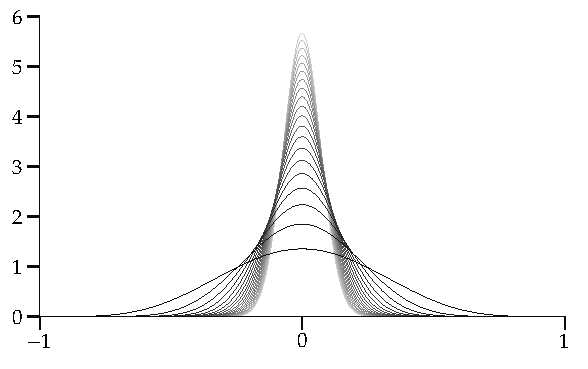
\includegraphics{figures/weierqn}
\caption{Plot of the approximate delta functions $q_n$ on $[-1,1]$ for
$n=5,10,15,20,\ldots,100$ with higher $n$ in lighter shade.\label{fig:weierqn}}
\end{myfigureht}

The functions $q_n$ are peaks around 0 (ignoring what happens outside
of $[-1,1]$) that get narrower and taller as $n$ increases,
while the area underneath is always 1.
A classic approximation idea
is to do a \emph{\myindex{convolution}} integral with peaks like this:
For
for $x \in [0,1]$, let
\begin{equation*}
p_n(x) := \int_{0}^1 g(t)q_n(x-t) \,dt \quad \left( = \int_{-\infty}^\infty
g(t)q_n(x-t) \,dt \right) .
\end{equation*}
The idea of this convolution is that we do a \myquote{weighted average} of the
function $g$ around the point $x$ using $q_n$ as the weight.
See \figureref{fig:approxdeltaconv}.

\begin{myfigureht}
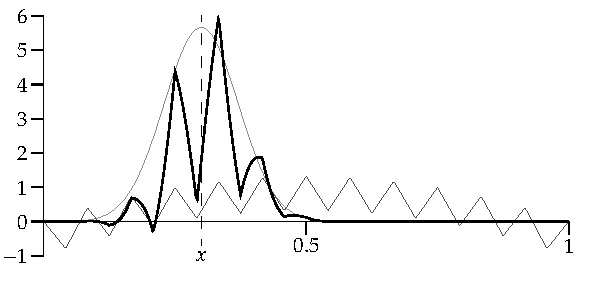
\includegraphics{figures/approxdeltaconv}
\caption{For $x=0.3$, the plot of $q_{100}(x-t)$ (light gray peak centered
at $x$), some continuous function
$g(t)$ (the jagged line) and the product $g(t)q_{100}(x-t)$ (the bold line).\label{fig:approxdeltaconv}}
\end{myfigureht}

As $q_n$ is a narrow peak, the integral
mostly sees the values of $g$ that are
close to $x$ and it does the weighted average of them.
When the peak gets narrower, we compute this average closer to $x$
and we expect the result to get closer to the value of $g(x)$.  Really we are
approximating what is called a delta function\footnote{The delta function
is not actually a function,
it is a \myquote{thing} that supposed to give
\myquote{$\int_{-\infty}^\infty g(x) \delta(x-t) \, dt = g(x)$.}}
(don't worry if you have not
heard of this concept),
and functions like $q_n$ are often called
\emph{approximate delta functions}\index{approximate delta function}.
We could do this with any set of polynomials that look like narrower
and narrower peaks near zero.  These just happen to be the simplest ones.
We only need this behavior on $[-1,1]$ as the convolution sees nothing
further than this as $g$ is zero outside $[0,1]$.

Because $q_n$ is a polynomial we write
\begin{equation*}
q_n(x-t) = a_0(t) + a_1(t)\,x + \cdots + a_{2n}(t)\, x^{2n} ,
\end{equation*}
where $a_k(t)$ are polynomials in $t$, in particular continuous and hence
integrable functions.
So
\begin{equation*}
\begin{split}
p_n(x) & =
\int_{0}^1 g(t)q_n(x-t) \,dt
\\
&=
\left(
\int_0^1
g(t)
a_0(t)\,dt
\right)
+
\left(
\int_0^1
g(t)
a_1(t)\,dt
\right)
\,
x
+
\cdots
+
\left(
\int_0^1
g(t)
a_{2n}(t)\,dt
\right)
\,
x^{2n} .
\end{split}
\end{equation*}
In other words, $p_n$ is a polynomial%
\footnote{%
Do note that the functions $a_j$ depend on $n$, so the coefficients of $p_n$
change as $n$ changes.}
 in $x$.
If $g(t)$ is real-valued, then the functions $g(t)a_j(t)$ are
real-valued and hence $p_n$ has real coefficients,
proving the \myquote{furthermore} part of the theorem.

We still need to prove that $\{ p_n \}$ converges to $g$.  First let us
get some handle on the size of $c_n$.
For $x \in [0,1]$, we have that $1-x \leq 1-x^2$.  We estimate
\begin{equation*}
\begin{split}
c_n^{-1}   = \int_{-1}^1 {(1-x^2)}^n \, dx
& = 2\int_0^1 {(1-x^2)}^n \, dx \\
& \geq 2\int_0^{1} {(1-x)}^n \, dx
= \frac{2}{n+1} .
\end{split}
\end{equation*}
So $c_n \leq \frac{n+1}{2} \leq n$.

Let us see how small $q_n$ is, if we ignore some small interval around the origin,
which is where the peak is.
Given any $\delta > 0$, $\delta < 1$, for
$x$ such that $\delta \leq \sabs{x} \leq 1$, we have
\begin{equation*}
q_n(x) \leq c_n {(1-\delta^2)}^n \leq  n{(1-\delta^2)}^n ,
\end{equation*}
because $q_n$ is increasing on $[-1,0]$ and decreasing on $[0,1]$.
By the ratio test, 
$n{(1-\delta^2)}^n$ goes to 0 as $n$ goes to infinity.

The function $q_n$ is even, $q_n(t) = q_n(-t)$, and $g$
is zero outside of $[0,1]$.
So for $x \in [0,1]$,
\begin{equation*}
p_n(x) = 
\int_{0}^1 g(t)q_n(x-t) \, dt
=
\int_{-x}^{1-x} g(x+t)q_n(-t) \, dt
=
\int_{-1}^{1} g(x+t)q_n(t) \, dt .
\end{equation*}

Let $\epsilon > 0$ be given.
As $[-1,2]$ is compact and $g$ is continuous on $[-1,2]$, we have that $g$ is uniformly continuous.
Pick $0 < \delta < 1$ such that if
$\sabs{x-y} < \delta$ (and $x,y \in [-1,2]$), then
\begin{equation*}
\sabs{g(x)-g(y)} < \frac{\epsilon}{2} .
\end{equation*}
Let $M$ be such that $\sabs{g(x)} \leq M$ for all $x$.  Let $N$ be
such that for all $n \geq N$,
\begin{equation*}
4M n{(1-\delta^2)}^n < \frac{\epsilon}{2} .
\end{equation*}
Note that 
$\int_{-1}^1 q_n(t) \, dt = 1$ and $q_n(t) \geq 0$ on $[-1,1]$.  So for $n
\geq N$ and every $x \in [0,1]$,
\begin{equation*}
\begin{split}
\sabs{p_n(x)-g(x)} & =
\abs{\int_{-1}^1 g(x+t)q_n(t) \, dt
-g(x)\int_{-1}^1 q_n(t) \, dt} \\
& =
\abs{\int_{-1}^1 \bigl(g(x+t)-g(x)\bigr)q_n(t) \, dt} \\
& \leq
\int_{-1}^1 \sabs{g(x+t)-g(x)} q_n(t) \, dt \\
& =
\int_{-1}^{-\delta} \sabs{g(x+t)-g(x)} q_n(t) \, dt
\quad +
\int_{-\delta}^{\delta} \sabs{g(x+t)-g(x)} q_n(t) \, dt
\\
& \phantom{\leq} +
\int_{\delta}^1 \sabs{g(x+t)-g(x)} q_n(t) \, dt \\
& \leq
2M
\int_{-1}^{-\delta} q_n(t) \, dt
\quad
+
\quad
\frac{\epsilon}{2}
\int_{-\delta}^{\delta} q_n(t) \, dt
\quad
+
\quad
2M
\int_{\delta}^1 q_n(t) \, dt \\
& \leq
2M n{(1-\delta^2)}^n(1-\delta)
\quad
+
\quad
\frac{\epsilon}{2}
\quad
+
\quad
2M n{(1-\delta^2)}^n(1-\delta) \\
& <
4M n{(1-\delta^2)}^n
+
\frac{\epsilon}{2}
< \epsilon . \qedhere
\end{split}
\end{equation*}
\end{proof}

A convolution often inherits some property of the functions we are convolving.
In our case the convolution $p_n$ inherited the property of being a
polynomial from $q_n$.  The same idea of the proof is often used 
to get other properties.  If $q_n$ or $g$ is infinitely differentiable, so is $p_n$.
If $q_n$ or $g$ is a solution to a linear differential equation, so is $p_n$.
Etc.

Let us note an immediate application of the Weierstrass theorem.  We have
already seen that countable dense subsets can be very useful.

\begin{cor}
The metric space $C([a,b],\C)$ contains a countable dense subset.
\end{cor}

\begin{proof}
Without loss of generality suppose that we are dealing with $C([a,b],\R)$
(why?).
The real polynomials are dense in $C([a,b],\R)$ by Weierstrass.  If we show that
every real polynomial can be approximated by polynomials with rational
coefficients, we are done.  This is because there are only countably many
rational numbers and so there are only countably many polynomials with
rational coefficients (a countable union of countable sets is still
countable).

Further without loss of generality, suppose $[a,b]=[0,1]$.  Let
\begin{equation*}
p(x) := \sum_{k=0}^n a_k\,  x^k
\end{equation*}
be a polynomial of degree $n$ where $a_k \in \R$.  Given $\epsilon > 0$, pick $b_k \in \Q$
such that $\sabs{a_k-b_k} < \frac{\epsilon}{n+1}$.  Then
if we let
\begin{equation*}
q(x) := \sum_{k=0}^n b_k \, x^k ,
\end{equation*}
we have
\begin{equation*}
\sabs{p(x)-q(x)}
=
\abs{\sum_{k=0}^n (a_k-b_k) x^k}
\leq
\sum_{k=0}^n \sabs{a_k-b_k} x^k
\leq
\sum_{k=0}^n \sabs{a_k-b_k}
<
\sum_{k=0}^n \frac{\epsilon}{n+1} = \epsilon . \qedhere
\end{equation*}
\end{proof}

\begin{remark}
While we will not prove this, the corollary above implies that
$C([a,b],\C)$ has the same cardinality as $\R$, which may be a
bit surprising.  The set of all functions $[a,b] \to \C$ has
cardinality that is strictly greater than the cardinality of $\R$, it has the
cardinality of the power set of $\R$.  So the
set of continuous functions is a very tiny subset of the set of all
functions.
\end{remark}

\textbf{Warning!}
The fact that every continuous function $f \colon [-1,1] \to \C$ (or any
interval $[a,b]$) can be uniformly
approximated by polynomials
\begin{equation*}
\sum_{k=0}^n a_k\,  x^k
\end{equation*}
does not mean that every continuous $f$ is analytic, that is, equal to a
power series
\begin{equation*}
\sum_{k=0}^\infty c_k\,  x^k .
\end{equation*}
An analytic function is infinitely differentiable, so the function
$\sabs{x}$ provides a counterexample.

The key distinction is that
the polynomials coming from the Weierstrass theorem are not the partial
sums of a power series.  For each one, the coefficients $a_k$ above can be
completely different---they do not need to come from a single sequence $\{
c_k \}$.

\subsection{Stone--Weierstrass approximation}

We want to abstract away what is not really
necessary and prove a general version of the Weierstrass theorem.
The polynomials are dense in the space of continuous
functions on a compact interval.  What other kind of families of
functions are also dense?  And if the domain is an
arbitrary metric space, then we no longer have polynomials
to begin with.

The theorem we will prove is the Stone--Weierstrass theorem\footnote{%
Named after the American mathematician
\href{https://en.wikipedia.org/wiki/Marshall_Harvey_Stone}{Marshall Harvey Stone}
(1903--1989), and the German mathematician
\href{https://en.wikipedia.org/wiki/Karl_Weierstrass}{Karl Theodor Wilhelm Weierstrass}
(1815--1897).}.
First,
we need a very
special case of the Weierstrass theorem though.

\begin{cor}
Let $[-a,a]$ be an interval.  Then there is a sequence of real polynomials
$\{ p_n \}$ that converges uniformly to $\sabs{x}$ on $[-a,a]$ and such that
$p_n(0) = 0$ for all $n$.
\end{cor}

\begin{proof}
As $f(x) := \sabs{x}$ is continuous and real-valued
on $[-a,a]$, the Weierstrass theorem gives a sequence of
real polynomials $\{ \widetilde{p}_n \}$ that converges to $f$
uniformly on $[-a,a]$.
Let
\begin{equation*}
p_n(x) := \widetilde{p}_n(x) - \widetilde{p}_n(0) .
\end{equation*}
Obviously $p_n(0) = 0$.

Given $\epsilon > 0$, let $N$ be such that
for $n \geq N$, we have
$\bigl\lvert\widetilde{p}_n(x)-\sabs{x}\big\rvert <
\nicefrac{\epsilon}{2}$ for all $x \in [-a,a]$.
In particular,
$\sabs{\widetilde{p}_n(0)} < \nicefrac{\epsilon}{2}$.
Then for $n \geq N$,
\begin{equation*}
\bigl\lvert p_n(x)-\sabs{x} \bigr\rvert
=
\bigl\lvert \widetilde{p}_n(x) - \widetilde{p}_n(0) - \sabs{x} \bigr\rvert
\leq
\bigl\lvert \widetilde{p}_n(x) - \sabs{x} \bigr\rvert + \sabs{\widetilde{p}_n(0)} < 
\nicefrac{\epsilon}{2} + \nicefrac{\epsilon}{2} = \epsilon . \qedhere
\end{equation*}
\end{proof}

Generalizing the corollary,
we can always make the polynomials from the Weierstrass theorem
be equal to our target function at one point, not just for $\sabs{x}$, but
that's the one we will need.

\begin{defn}
A set $\sA$ of complex-valued functions $f \colon X \to \C$ is said to be an 
\emph{\myindex{algebra}} (sometimes
\emph{\myindex{complex algebra}} or \emph{algebra over $\C$}) if for all $f,
g \in \sA$ and $c \in \C$, we have
\begin{enumerate}[(i)]
\item $f+g \in \sA$.
\item $fg \in \sA$.
\item $cg \in \sA$.
\end{enumerate}
A \emph{\myindex{real algebra}} or an
\emph{algebra over $\R$} is a set of real-valued
functions that satisfies the three properties above for $c \in \R$.
\end{defn}

We are interested in the case when
$X$ is a compact metric space.  Then
$C(X,\C)$ and $C(X,\R)$ are metric spaces.
Given a set $\sA \subset C(X,\C)$, the set of all uniform
limits is the metric space closure $\widebar{\sA}$.
When we talk about closure of an algebra
from now on we mean the closure in $C(X,\C)$
as a metric space.  Same for $C(X,\R)$.

The set $\sP$ of all polynomials is an algebra in
$C([a,b],\C)$, and we
have shown that its closure $\widebar{\sP} = C([a,b],\C)$.
That is, it is dense.  That is the sort of result that we wish to prove.

We leave the following proposition as an exercise.

\begin{prop} \label{prop:closureofalgebra}
Suppose $X$ is a compact metric space.
If $\sA \subset C(X,\C)$ is an algebra, then the closure $\widebar{\sA}$ is also an algebra.
Similarly for a real algebra in $C(X,\R)$.
\end{prop}

Let us distill the properties of polynomials that are sufficient
for an approximation theorem.

\begin{defn}
Let $\sA$ be a set of complex-valued functions defined on a set $X$.
\begin{enumerate}[(i)]
\item $\sA$ \emph{\myindex{separates points}}
if for every $x,y \in X$, with $x \not= y$ there is a function $f \in \sA$ such that
$f(x) \not= f(y)$.
\item 
$\sA$ \emph{\myindex{vanishes at no point}} if for every $x \in X$
there is an $f \in \sA$ such that $f(x) \not= 0$.
\end{enumerate}
\end{defn}

\begin{example}
The set $\sP$ of polynomials separates points and vanishes at no point
on $\R$.  That is, $1 \in \sP$ so it vanishes at no point.  And for $x,y \in
\R$, $x\not= y$, take $f(t) := t$.  Then $f(x) = x \not= y = f(y)$.
So $\sP$ separates points.
\end{example}

\begin{example}
The set of functions of the form
\begin{equation*}
f(t) = a_0 + \sum_{n=1}^k a_n \cos(nt)
\end{equation*}
is an algebra,
which follows by the identity $\cos(mt)\cos(nt) = 
\frac{\cos((n+m) t)}{2}+
\frac{\cos((n-m) t)}{2}$.
The algebra
does not separate points if the domain is an interval of the form
$[-a,a]$, because $f(-t) = f(t)$ for all $t$.
It does separate points if the domain is $[0,\pi]$, as $\cos(t)$
is one-to-one on that set.
\end{example}

\begin{example}
The set of polynomials with no constant term vanishes at the origin.
\end{example}

\begin{prop} \label{prop:SWinterpolate}
Suppose $\sA$ is an algebra of complex-valued functions on a set $X$, that separates points
and vanishes at no point.  Suppose $x,y$ are distinct points of $X$, and
$c,d \in \C$.  Then there is an $f \in \sA$ such that
\begin{equation*}
f(x) = c, \qquad f(y) = d .
\end{equation*}
If $\sA$ is a real algebra, the conclusion holds for $c,d \in \R$.
\end{prop}

\begin{proof}
There must exist an $g,h,k \in \sA$
such that 
\begin{equation*}
g(x) \not= g(y), \quad h(x) \not= 0, \quad k(y) \not= 0 .
\end{equation*}
Let
\begin{equation*}
f := 
c
\frac{\bigl(g - g(y)\bigr)h}{\bigl(g(x)-g(y)\bigr)h(x) } + 
d
\frac{\bigl(g - g(x)\bigr)k}{\bigl(g(y)-g(x)\bigr)k(y)}
=
c
\frac{gh - g(y)h}{g(x)h(x)-g(y)h(x) } + 
d
\frac{gk - g(x)k}{g(y)k(y)-g(x)k(y)} .
\end{equation*}
Do note that we are not dividing by zero (clear from the first formula).
Also from the first formula we see that $f(x) = c$ and $f(y) = d$.
By the second formula we see that $f \in \sA$ (as $\sA$ is an algebra).
\end{proof}

\begin{thm}[Stone--Weierstrass, real version]
\label{thm:SWreal}%
\index{Stone--Weierstrass!real version}%
Let $X$ be a compact metric space and $\sA$ an algebra of real-valued
continuous functions on $X$, such that $\sA$ separates points and vanishes at
no point.  Then the closure $\widebar{\sA} = C(X,\R)$.
\end{thm}

The proof is divided into several claims.

\medskip

\noindent
\textbf{Claim 1:} \emph{If $f \in \widebar{\sA}$, then $\sabs{f} \in
\widebar{\sA}$.}

\begin{proof}
The function $f$ is bounded (continuous on a compact set), so there is an $M$
such that $\sabs{f(x)} \leq M$ for all $x \in X$.

Let $\epsilon > 0$ be given.  By the corollary to the Weierstrass theorem there
exists a real polynomial $c_1 y + c_2 y^2 + \cdots+ c_n y^n$ (vanishing at
$y=0$) such that
\begin{equation*}
\abs{\sabs{y} - \sum_{j=1}^N c_j y^j} < \epsilon
\end{equation*}
for all $y \in [-M,M]$.
Because $\widebar{\sA}$ is an algebra and because there is no constant term in the
polynomial,
\begin{equation*}
\sum_{j=1}^N c_j f^j \in \widebar{\sA} .
\end{equation*}
As $\sabs{f(x)} \leq M$, then  for all $x \in X$
\begin{equation*}
\abs{\sabs{f(x)} - \sum_{j=1}^N c_j {\bigl(f(x)\bigr)}^j}
< \epsilon .
\end{equation*}
So $\sabs{f}$ is in the closure of $\widebar{\sA}$, which is closed.
In other words, $\sabs{f} \in \widebar{\sA}$.
\end{proof}

\medskip

\noindent
\textbf{Claim 2:} \emph{If $f \in \widebar{\sA}$ and $g \in \widebar{\sA}$, then
$\max(f,g) \in \widebar{\sA}$ and
$\min(f,g) \in \widebar{\sA}$, where
}
\begin{equation*}
\bigl(\max(f,g)\bigr) (x) := \max \bigl\{ f(x), g(x) \bigr\} , \qquad
\text{and} \qquad
\bigl(\min(f,g)\bigr) (x) := \min \bigl\{ f(x), g(x) \bigr\} .
\end{equation*}

\begin{proof}
Write:
\begin{equation*}
\max(f,g) = \frac{f+g}{2} + \frac{\sabs{f-g}}{2} ,
\end{equation*}
and
\begin{equation*}
\min(f,g) = \frac{f+g}{2} - \frac{\sabs{f-g}}{2} .
\end{equation*}
As $\widebar{\sA}$ is an algebra we are done.
\end{proof}

The claim is true for the minimum or maximum of every finite
collection of functions as well.

\medskip

\noindent
\textbf{Claim 3:} \emph{Given $f \in C(X,\R)$, $x \in X$ and $\epsilon > 0$
there exists a $g_x \in \widebar{\sA}$ with $g_x(x) = f(x)$ and
}
\begin{equation*}
g_x(t) > f(t)-\epsilon \qquad \text{for all } t \in X.
\end{equation*}

\begin{proof}
Fix $f$, $x$, and $\epsilon$.
By \propref{prop:SWinterpolate}, for every $y \in X$ we find an $h_y \in
\sA$ such that
\begin{equation*}
h_y(x) = f(x), \qquad h_y(y)=f(y) .
\end{equation*}
As $h_y$ and $f$ are continuous, the function $h_y-f$ is continuous,
and the set
\begin{equation*}
U_y :=
\bigl\{ t \in X : h_y(t) > f(t) -\epsilon \bigr\}
=
{(h_y-f)}^{-1} \bigl( (-\epsilon,\infty) \bigr)
\end{equation*}
is open (it is the inverse image of an open set by a continuous function).
Furthermore $y \in U_y$.  So the sets $U_y$ cover $X$.

The space $X$ is compact so there exist finitely many
points $y_1,y_2,\ldots,y_n$ in $X$ such
that
\begin{equation*}
X = \bigcup_{j=1}^n U_{y_j}  .
\end{equation*}
Let 
\begin{equation*}
g_x := \max(h_{y_1},h_{y_2},\ldots,h_{y_n}) .
\end{equation*}
By Claim 2, $g_x \in \widebar{\sA}$.
Furthermore,
\begin{equation*}
g_x(t) > f(t) -\epsilon
\end{equation*}
for all $t \in X$, since for every $t$, there is a $y_j$ such that 
$t \in U_{y_j}$, and so 
$h_{y_j}(t) > f(t) -\epsilon$.

Finally $h_y(x) = f(x)$ for all $y \in X$, so
$g_x(x) = f(x)$.
\end{proof}

\medskip

\noindent
\textbf{Claim 4:} \emph{If $f \in C(X,\R)$ and $\epsilon > 0$ is given, then there
exists an $\varphi \in \widebar{\sA}$ such that}
\begin{equation*}
\sabs{f(x) - \varphi(x)} < \epsilon .
\end{equation*}

\begin{proof}
For every $x$ find the function $g_x$ as in Claim 3.

Let
\begin{equation*}
V_x := \bigl\{ t \in X : g_x(t) < f(t) + \epsilon \bigr\}.
\end{equation*}
The sets $V_x$ are open as $g_x$ and $f$ are continuous.
As $g_x(x) = f(x)$, then $x \in V_x$.  So the sets $V_x$ cover $X$.
By compactness of $X$,
there
are finitely many points $x_1,x_2,\ldots,x_k$ such that
\begin{equation*}
X = \bigcup_{j=1}^k V_{x_j} .
\end{equation*}
Let
\begin{equation*}
\varphi := \min(g_{x_1},g_{x_2},\ldots,g_{x_k}) .
\end{equation*}
By Claim 2, $\varphi \in \widebar{\sA}$.  Similarly as before (same argument as in
Claim 3), for all $t \in X$,
\begin{equation*}
\varphi(t) < f(t) + \epsilon .
\end{equation*}
Since all the $g_x$ satisfy $g_x(t) > f(t) - \epsilon$ for all $t \in X$,
$\varphi(t) > f(t) - \epsilon$ as well.
Therefore, for all $t$,
\begin{equation*}
-\epsilon < \varphi(t) - f(t) < \epsilon ,
\end{equation*}
which is the desired conclusion.
\end{proof}

The proof of the theorem follows from Claim 4.  The claim states that an
arbitrary continuous function is in the closure of $\widebar{\sA}$,
which itself is
closed.  So the theorem is proved.

\begin{example}
The functions of the form
\begin{equation*}
f(t) = \sum_{j=1}^n c_j \, e^{jt},
\end{equation*}
for $c_j \in \R$,
are dense in $C([a,b],\R)$.  We need to note that such functions are a real
algebra, which follows from $e^{jt} e^{kt} = e^{(j+k)t}$.  They separate
points as $e^t$ is one-to-one, and $e^t > 0$ for all $t$ so the algebra
does not vanish at any point.
\end{example}

In general if we have a set of functions that separates points and does
not vanish at any point, we can let these functions
\emph{generate}\index{generate an algebra}
an algebra
by considering all the linear combinations of arbitrary multiples of such
functions.  That is, we consider all real polynomials without constant term
of such functions.  In the example above,
the algebra is generated by $e^t$.  We 
consider polynomials in $e^t$ without constant term.

\begin{example}
We mentioned that the set of all functions of the form
\begin{equation*}
a_0 +
\sum_{n=1}^N a_n \cos(nt)
\end{equation*}
is an algebra.
When considered on $[0,\pi]$, 
it separates points and vanishes nowhere so
\hyperref[thm:SWreal]{Stone--Weierstrass} applies.
As for polynomials, you \emph{do not} want to conclude that every continuous
function on $[0,\pi]$ has a uniformly convergent
Fourier cosine series, that is, that every continuous
function can be written as
\begin{equation*}
a_0 +
\sum_{n=1}^\infty a_n \cos(nt) .
\end{equation*}
That is \emph{not true}!
There exist continuous functions
whose Fourier series does not converge even pointwise
let alone uniformly.
\end{example}

To obtain Stone--Weierstrass for complex algebras, we must
make an extra assumption.

\begin{defn}
An algebra $\sA$ is \emph{\myindex{self-adjoint}} if for all $f \in \sA$, the function
$\bar{f}$ defined by $\bar{f}(x) := \overline{f(x)}$ is in $\sA$, where by the
bar we mean the complex conjugate.
\end{defn}

\begin{thm}[Stone--Weierstrass, complex version]
\label{thm:SWcomplex}%
\index{Stone--Weierstrass!complex version}%
Let $X$ be a compact metric space and $\sA$ an algebra of complex-valued
continuous functions on $X$, such that $\sA$ separates points, vanishes at
no point, and is self-adjoint.  Then the closure $\widebar{\sA} = C(X,\C)$.
\end{thm}

\begin{proof}
Suppose $\sA_\R \subset \sA$ is the set of the real-valued elements of
$\sA$.
For $f \in \sA$, write $f = u+iv$ where $u$ and $v$ are real-valued.
Then
\begin{equation*}
u = \frac{f+\bar{f}}{2}, \qquad
v = \frac{f-\bar{f}}{2i} .
\end{equation*}
So $u, v \in \sA$ as $\sA$ is a self-adjoint algebra, and since they are
real-valued $u, v \in \sA_\R$.

If $x \not= y$, then find an $f \in \sA$ such that $f(x) \not= f(y)$.  If $f
= u+iv$, then it is obvious that either $u(x) \not= u(y)$ or $v(x) \not=
v(y)$.  So $\sA_\R$ separates points.

Similarly, for every $x$ find $f \in \sA$ such that $f(x) \not= 0$.  If $f
= u+iv$, then either $u(x) \not= 0$ or $v(x) \not= 0$.
So $\sA_\R$ vanishes at no point.

The set $\sA_\R$ is a real algebra, and satisfies the hypotheses of the
\hyperref[thm:SWreal]{real Stone--Weierstrass theorem}.
Given any $f = u+iv \in C(X,\C)$,
we find $g,h \in \sA_\R$ such that
$\sabs{u(t)-g(t)} < \nicefrac{\epsilon}{2}$ and
$\sabs{v(t)-h(t)} < \nicefrac{\epsilon}{2}$ for all $t \in X$.
Next, $g+i h \in \sA$, and
\begin{multline*}
\abs{f(t) - \bigl(g(t)+ih(t)\bigr)} = 
\abs{u(t)+iv(t) - \bigl(g(t)+ih(t)\bigr)} \\
\leq
\sabs{u(t)-g(t)}+\sabs{v(t)-h(t)} < \nicefrac{\epsilon}{2} +
\nicefrac{\epsilon}{2} = \epsilon
\end{multline*}
for all $t \in X$.
So $\widebar{\sA} = C(X,\C)$.
\end{proof}

The self-adjoint requirement is necessary although it is not so obvious to
see it.  For an example see \exerciseref{exercise:selfadjointSW}.

Here is an interesting application.
When working
with functions of two variables, it may be useful to work with functions
of the form $f(x)g(y)$ rather than $F(x,y)$.  For example, they are easier
to integrate.  We have the following.

\begin{example}
Any continuous function $F \colon [0,1] \times [0,1] \to \C$ can be
approximated uniformly by functions of the form
\begin{equation*}
\sum_{j=1}^n f_j(x) g_j(y) ,
\end{equation*}
where $f_j \colon [0,1] \to \C$ and $g_j \colon [0,1] \to \C$ are continuous.

Proof:
It is not hard to see that the functions of the above form are a complex
algebra.  It is equally easy to show that they vanish nowhere, separate
points, and the algebra is self-adjoint.  As $[0,1] \times [0,1]$ is compact
we apply \hyperref[thm:SWcomplex]{Stone--Weierstrass} to obtain the result.
\end{example}

\subsection{Exercises}

\begin{exercise}
Prove \propref{prop:closureofalgebra}.
Hint: If $\{ f_n \}$ is a sequence in $C(X,\R)$
converging to $f$, then as $f$ is bounded, you can show
that $f_n$ is uniformly bounded, that is, there exists a
single bound for all $f_n$ (and $f$).
\end{exercise}

\begin{exercise}
Suppose $X := \R$ (not compact in particular).
Show that $f(t) := e^t$ is not possible to uniformly approximate
by polynomials on $X$.  Hint: Consider $\abs{\frac{e^t}{t^n}}$
as $t \to \infty$.
\end{exercise}

\begin{exercise}
Suppose $f \colon [0,1] \to \C$ is a uniform limit of a sequence of polynomials
of degree at most $d$, then the limit is a polynomial of degree at most $d$.
Conclude that to approximate a function which is not a polynomial, we
need the degree of the approximations to go to infinity.\\
Hint: First prove that if a sequence of polynomials of degree $d$
converges uniformly to the zero function, then 
the coefficients converge to zero.
One way to do this is linear algebra: Consider a polynomial $p$
evaluated at $d+1$ points
to be a linear operator taking the
coefficients of $p$ to the values of $p$
(an operator in $L(\R^{d+1})$).
\end{exercise}

\begin{exercise}
Suppose $f \colon [0,1] \to \R$ is continuous and
$\int_0^1 f(x) x^n \, dx = 0$ for all $n = 0,1,2,\ldots$.
Show that $f(x) = 0$ for all $x \in [0,1]$.
Hint: Approximate by polynomials to show that $\int_0^1 {\bigl( f(x)
\bigr)}^2 \, dx = 0$.
\end{exercise}

\begin{exercise}
Suppose $I \colon C([0,1],\R) \to \R$ is 
a linear continuous function such that
$I(x^n) = \frac{1}{n+1}$
for all $n=0,1,2,3,\ldots$.
Prove that $I(f) = \int_0^1 f$ for all $f \in C([0,1],\R)$.
\end{exercise}

\begin{exercise}
Let $\sA$ be the collection of real polynomials in $x^2$,
that is polynomials of the form
$c_0 + c_1 x^2 + c_2 x^4 + \cdots + c_d x^{2d}$.
\begin{enumerate}[a)]
\item
Show that every $f \in C([0,1],\R)$ is a uniform limit of
polynomials from $\sA$.
\item
Find an $f \in  C([-1,1],\R)$ that is not a
uniform limit of
polynomials from $\sA$.
\item
Which hypothesis of the real Stone--Weierstrass is not satisfied
for the domain $[-1,1]$?
\end{enumerate}
\end{exercise}

\begin{exercise}
\pagebreak[2]
Let $\sabs{z}=1$ define the unit circle $S^1 \subset \C$.
\begin{enumerate}[a)]
\item
Show that functions of the form
\begin{equation*}
\sum_{k=-n}^n c_k\, z^k
\end{equation*}
are dense in $C(S^1,\C)$.  Notice the negative powers.
\item 
Show that functions of the form
\begin{equation*}
c_0
+
\sum_{k=1}^n c_k \, z^k
+
\sum_{k=1}^n c_{-k}\, \bar{z}^k
\end{equation*}
are dense in $C(S^1,\C)$.  These are so-called harmonic polynomials,
and this approximation leads to, for example, the solution of the
steady state heat problem.
\end{enumerate}
Hint: A good way to write the equation for $S^1$ is $z \bar{z} = 1$.
\end{exercise}

\begin{exercise}
Show that for complex numbers $c_j$, the set of functions
of $x$ on $[-\pi,\pi]$
of the form
\begin{equation*}
\sum_{k=-n}^n c_k \, e^{ik x}
\end{equation*}
satisfies the hypotheses of the complex Stone--Weierstrass theorem
and therefore such functions are dense in the $C([-\pi,\pi],\C)$.
\end{exercise}

\begin{exercise} \label{exercise:selfadjointSW}
Let $S^1 \subset \C$ be the unit circle, that is the set where
$\sabs{z} = 1$.  Orient this set counterclockwise.
Let $\gamma(t) := e^{it}$.
For the one-form $f(z)\,dz$ we write\footnote{%
One could also define $dz := dx + i \, dy$ and then
extend the path integral from \chapterref{path:chapter} to complex-valued
one-forms.}
\begin{equation*}
\int_{S^1} f(z) \,dz := \int_0^{2\pi} f(e^{it}) \, i e^{it} \, dt . 
\end{equation*}
\begin{enumerate}[a)]
\item
Prove that for all nonnegative integers $k = 0,1,2,3,\ldots$, we have
$\int_{S^1} z^k \, dz = 0$.
\item
Prove that if
$P(z) = \sum_{k=0}^n c_k z^k$ is a
polynomial in $z$, then
$\int_{S^1} P(z) \, dz = 0$.
\item
Prove
$\int_{S^1} \bar{z} \, dz \not= 0$.
\item
Conclude that polynomials in $z$ (this algebra of functions is
not self-adjoint) are not dense in $C(S^1,\C)$.
\end{enumerate}
\end{exercise}

\begin{exercise}
Let $(X,d)$ be a compact metric space and
suppose $\sA \subset C(X,\R)$ is a real algebra that separates points, but
such that for some $x_0$, $f(x_0) = 0$ for all $f \in \sA$.  Prove that
every function $g \in C(X,\R)$ such that $g(x_0) = 0$ is a uniform limit
of functions from $\sA$.
\end{exercise}

\begin{exercise}
Let $(X,d)$ be a compact metric space and
suppose $\sA \subset C(X,\R)$ is a real algebra.
Suppose that for each $y \in X$ the closure $\widebar{\sA}$
contains the function $\varphi_y(x) := d(y,x)$.
Then $\widebar{\sA} = C(X,\R)$.
\end{exercise}

\begin{exercise}
\leavevmode
\begin{enumerate}[a)]
\item
Suppose $f \colon [a,b] \to \C$ is continuously 
differentiable.  Show that there exists a sequence of polynomials
$\{ p_n \}$
that converges in the $C^1$ norm to $f$, that is
$\snorm{f - p_n}_u + \snorm{f'-p_n'}_u \to 0$ as $n \to \infty$.
\item
Suppose $f \colon [a,b] \to \C$ is $k$ times continuously 
differentiable.  Show that there exists a sequence of polynomials
$\{ p_n \}$
that converges in the $C^k$ norm to $f$, that is,
\begin{equation*}
\sum_{j=0}^k \snorm{f^{(j)} - p_n^{(j)}}_u \to 0 \qquad \text{as} \qquad
n \to \infty.
\end{equation*}
\end{enumerate}
\end{exercise}

\begin{exercise}
\leavevmode
\begin{enumerate}[a)]
\item
Show that an even function $f \colon [-1,1] \to \R$ is a uniform
limit of polynomials with even powers only, that is, polynomials
of the form $a_0 + a_1 x^2 + a_2 x^4 + \cdots + a_k x^{2k}$.
\item
Show that an odd function $f \colon [-1,1] \to \R$ is a uniform
limit of polynomials with odd powers only, that is, polynomials
of the form $b_1 x + b_2 x^3 + b_3 x^5 + \cdots + b_k x^{2k-1}$.
\end{enumerate}
\end{exercise}

%%%%%%%%%%%%%%%%%%%%%%%%%%%%%%%%%%%%%%%%%%%%%%%%%%%%%%%%%%%%%%%%%%%%%%%%%%%%%%

\sectionnewpage
\section{Fourier series}
\label{sec:fourier}

\sectionnotes{3--4 lectures}

Fourier series\footnote{%
Named after the French mathematician
\href{https://en.wikipedia.org/wiki/Joseph_Fourier}{Jean-Baptiste Joseph Fourier}
(1768--1830).} is perhaps the most important (and most difficult to
understand) of the series that we cover in
this book.  We have seen it in a few examples before, but let us start
at the beginning.

\subsection{Trigonometric polynomials}

A \emph{\myindex{trigonometric polynomial}} is an expression of the form
\begin{equation*}
a_0 + \sum_{n=1}^N \bigl(a_n \cos(nx) + b_n \sin(nx) \bigr),
\end{equation*}
or equivalently, thanks to Euler's formula ($e^{i\theta} = \cos(\theta) + i
\sin(\theta)$):
\begin{equation*}
\sum_{n=-N}^N c_n e^{inx} .
\end{equation*}
The second form is usually more convenient.  If
$z \in \C$ with $\sabs{z}=1,$ we write $z = e^{ix}$, and so
\begin{equation*}
\sum_{n=-N}^N c_n e^{inx} = 
\sum_{n=-N}^N c_n z^n .
\end{equation*}
So a trigonometric polynomial is really a rational function
of the complex variable $z$
(we are allowing negative powers) evaluated on the unit circle.  There is
a wonderful connection between power series (actually Laurent series because
of the negative powers) and
Fourier series because of this observation,
but we will not investigate this further.

\medskip

Another reason why Fourier series are important and come up in so many
applications is that the functions are eigenfunctions%
\footnote{Eigenfunction is like an eigenvector for a matrix, but for a linear
operator on a vector space of functions.} of various
differential operators.  For example,
\begin{equation*}
\frac{d}{dx} \bigl[ e^{ikx} \bigr] = (ik) e^{ikx}, \qquad
\frac{d^2}{dx^2} \bigl[ e^{ikx} \bigr] = (-k^2) e^{ikx} .
\end{equation*}
That is, they are the functions whose derivative is a scalar (the
eigenvalue) times itself.
Just as eigenvalues and eigenvectors are important in studying matrices,
eigenvalues and eigenfunctions are important when studying linear
differential equations.

\medskip

The functions $\cos (nx)$, $\sin (nx)$, and $e^{inx}$ are $2\pi$-periodic
and hence trigonometric
polynomials are also $2\pi$-periodic.
We could rescale $x$ to make the period different, but the theory is the
same, so let us stick with the period of $2\pi$.
The antiderivative of $e^{inx}$ is $\frac{e^{inx}}{in}$ and
so
\begin{equation*}
\int_{-\pi}^\pi e^{inx} \, dx =
\begin{cases}
2\pi & \text{if } n=0, \\
0    & \text{otherwise.}
\end{cases}
\end{equation*}
Consider
\begin{equation*}
f(x) := \sum_{n=-N}^N c_n e^{inx} ,
\end{equation*}
and for $m=-N,\ldots,N$ compute
\begin{equation*}
\frac{1}{2\pi} \int_{-\pi}^\pi
f(x) e^{-imx} \, dx
=
\frac{1}{2\pi} \int_{-\pi}^\pi
\left(\sum_{n=-N}^N c_n e^{i(n-m)x}\right) \, dx
=
\sum_{n=-N}^N
c_n
\frac{1}{2\pi}
\int_{-\pi}^\pi
e^{i(n-m)x}
 \, dx
=
c_m .
\end{equation*}
We just found a way of computing the coefficients $c_m$ using an integral
of $f$.  If $\sabs{m} > N$, the integral is just 0: We might as
well have included enough zero coefficients to make $\sabs{m} \leq N$.

\begin{prop}
A trigonometric polynomial
$f(x) = \sum_{n=-N}^N c_n\, e^{inx}$
is real-valued for real $x$ if
and only if $c_{-m} = \overline{c_m}$ for all $m=-N,\ldots,N$.
\end{prop}

\begin{proof}
If $f(x)$ is real-valued, that is $\overline{f(x)} = f(x)$, then
\begin{equation*}
\overline{c_m}
=
\overline{
\frac{1}{2\pi} \int_{-\pi}^\pi
f(x) e^{-imx} \, dx
}
=
\frac{1}{2\pi} \int_{-\pi}^\pi
\overline{
f(x) e^{-imx} } \, dx
=
\frac{1}{2\pi} \int_{-\pi}^\pi
f(x) e^{imx} \, dx
= c_{-m} .
\end{equation*}
The complex conjugate goes inside the integral because the integral is
done on real and imaginary parts separately.

On the other hand if 
$c_{-m} = \overline{c_m}$, then
\begin{equation*}
\overline{c_{-m}\, e^{-imx}+ c_{m}\, e^{imx}}
=
\overline{c_{-m}}\, e^{imx}+ \overline{c_{m}}\, e^{-imx}
=
c_{m}\, e^{imx}+ c_{-m}\, e^{-imx} ,
\end{equation*}
which is real valued.  Also $c_0 = \overline{c_0}$, so
$c_0$ is real.
By pairing up the terms we obtain that $f$ has to be real-valued.
\end{proof}

The functions $e^{inx}$ are also linearly independent.

\begin{prop}
If
\begin{equation*}
\sum_{n=-N}^N c_n \, e^{inx} = 0
\end{equation*}
for all $x \in [-\pi,\pi]$, then $c_n = 0$ for all $n$.
\end{prop}

\begin{proof}
The result follows immediately from the integral formula for $c_n$.
\end{proof}

\subsection{Fourier series}

We now take limits.  We call the series
\begin{equation*}
\sum_{n=-\infty}^\infty c_n \, e^{inx}
\end{equation*}
the \emph{\myindex{Fourier series}}.  The numbers $c_n$
are called \emph{\myindex{Fourier coefficients}}.  Using
Euler's formula $e^{i\theta} = \cos(\theta) + i \sin (\theta)$,
we could also develop everything with
sines and cosines, that is, as the series
$a_0 + \sum_{n=1}^\infty a_n \cos(nx) + b_n \sin(nx)$,
but it is equivalent and slightly more messy.

Several questions arise.  What functions are expressible as 
Fourier series?  Obviously, they have to be $2\pi$-periodic, but not every
periodic function is expressible with the series.  Furthermore, if we do have
a Fourier series, where does it converge (where and if at all)?  Does it converge
absolutely?  Uniformly?  Also note that the series has two
limits.  When talking about Fourier series convergence, we often
talk about the following limit:
\begin{equation*}
\lim_{N\to\infty} 
\sum_{n=-N}^N c_n e^{inx} .
\end{equation*}
There are other ways we can sum the series that can get convergence in more
situations, but we refrain from discussing those.

\medskip

Conversely, we start with an integrable function $f \colon [-\pi,\pi] \to
\C$, and we call the numbers
\begin{equation*}
c_n := 
\frac{1}{2\pi} \int_{-\pi}^\pi
f(x) e^{-inx} \, dx
\end{equation*}
its \emph{Fourier coefficients}.  Often these numbers are
written as $\hat{f}(n)$.\footnote{The notation seems similar
to Fourier transform for those readers that have seen it.
The similarity is not just
coincidental, we are taking a type of Fourier transform here.}
We then formally write down a Fourier series.
As you might imagine such a series might not even converge.
We write\glsadd{not:FS}
\begin{equation*}
f(x) \sim
\sum_{n=-\infty}^\infty c_n \, e^{inx} ,
\end{equation*}
although the $\sim$ doesn't imply anything about the two sides being equal
in any way.  It is simply that we created a formal series using the formula
for the coefficients.

A few sections ago, we proved that the Fourier series 
\begin{equation*}
\sum_{n=1}^\infty \frac{\sin(nx)}{n^2}
\end{equation*}
converges uniformly and hence converges to a continuous function.  This 
example and its proof can be extended to a more general criterion.

\begin{prop}
Let $\sum_{n=-\infty}^\infty c_n\, e^{inx}$ be a Fourier series,
and $C$, $\alpha > 1$ constants such that
\begin{equation*}
\sabs{c_n} \leq \frac{C}{\sabs{n}^\alpha}
\qquad \text{for all } n \in \Z \setminus \{ 0 \}.
\avoidbreak
\end{equation*}
Then the series converges (absolutely and uniformly) to a continuous function on $\R$.
\end{prop}

The proof is to apply the Weierstrass $M$-test (\thmref{thm:weiermtest}) and
the $p$-series test, to find that the series converges uniformly and hence
to a continuous function (\corref{cor:metricuniformcontinuous}).
We can also take derivatives.

\begin{prop}
Let $\sum_{n=-\infty}^\infty c_n\, e^{inx}$ be a Fourier series,
and $C$, $\alpha > 2$ constants such that
\begin{equation*}
\sabs{c_n} \leq \frac{C}{\sabs{n}^\alpha}
\qquad \text{for all } n \in \Z \setminus \{ 0 \}.
\avoidbreak
\end{equation*}
Then the series converges to a continuously differentiable function on $\R$.
\end{prop}

The trick is to first notice that the series converges first to a continuous
function by the previous proposition, so in particular it converges at some
point.  Then differentiate the partial sums
\begin{equation*}
\sum_{n=-N}^{N}
i n c_n \,e^{inx}
\end{equation*}
and notice that for all nonzero $n$
\begin{equation*}
\sabs{i n c_n} \leq \frac{C}{\sabs{n}^{\alpha-1}} .
\end{equation*}
The differentiated series converges uniformly by the $M$-test again.  Since
the differentiated series
converges uniformly, we find that the original series $\sum c_n\,e^{inx}$
converges 
to a continuously differentiable function, whose derivative is
the differentiated series (see \thmref{thm:dersconvergecomplex}).

We can iterate the same reasoning.
Suppose there is
some $C$ and $\alpha > k+1$ ($k \in \N$) such that
\begin{equation*}
\sabs{c_n} 
\leq \frac{C}{\sabs{n}^\alpha}
\end{equation*}
for all nonzero integers $n$.  Then 
the Fourier series converges to a $k$-times continuously differentiable
function.  Therefore, the faster the coefficients go to zero, the more
regular the limit is.

\subsection{Orthonormal systems}

Let us abstract away some of the properties of the exponentials, and
study a more general series for a function.
One fundamental property of the exponentials that make Fourier series what it 
is that the exponentials are a so-called \emph{orthonormal system}.
Let us fix an interval $[a,b]$.  We define an
\emph{\myindex{inner product}} for the space of functions.  We restrict our attention
to Riemann integrable functions since we do not have the Lebesgue
integral, which
would be the natural choice.  Let $f$ and $g$ be complex-valued 
Riemann integrable functions on $[a,b]$ and define the inner product
\glsadd{not:L2innprod}
\begin{equation*}
\langle f , g \rangle :=
\int_a^b f(x) \overline{g(x)} \, dx .
\end{equation*}
If you have seen Hermitian inner products in linear algebra, this
is precisely such a product.  We have to put in the conjugate as we are
working with complex numbers.  We then have the \myquote{size,} that is the
$L^2$ norm $\snorm{f}_2$ by (defining the square)
\glsadd{not:L2norm}
\begin{equation*}
\snorm{f}_2^2 :=
\langle f , f \rangle =
\int_a^b \sabs{f(x)}^2 \, dx .
\end{equation*}

\begin{remark}
Notice the similarity to finite dimensions.
For $z = (z_1,z_2,\ldots,z_n) \in \C^n$, we define 
\begin{equation*}
\langle z , w \rangle :=
\sum_{k=1}^n z_k \overline{w_k} .
\end{equation*}
Then the norm is (usually denoted by simply $\snorm{z}$ in $\C^n$
rather than $\snorm{z}_2$)
\begin{equation*}
\snorm{z}^2 = 
\langle z , z \rangle =
\sum_{k=1}^n \sabs{z_k}^2 .
\end{equation*}
This is just the euclidean distance to the origin in $\C^n$ (same as
$\R^{2n}$).
\end{remark}

Let us get back to function spaces.  In what follows, we will
assume all functions are Riemann integrable.

\begin{defn}
Let $\{ \varphi_n \}$ be a sequence of integrable complex-valued
functions on $[a,b]$.  We say that this is an
\emph{\myindex{orthonormal system}} if
\begin{equation*}
\langle \varphi_n , \varphi_m \rangle
=
\int_a^b \varphi_n(x) \, \overline{\varphi_m(x)} \, dx
= 
\begin{cases}
1 & \text{if } n=m, \\
0 & \text{otherwise.}
\end{cases}
\end{equation*}
In particular, $\snorm{\varphi_n}_2 = 1$ for all $n$.  If we
only require that 
$\langle \varphi_n , \varphi_m \rangle = 0$ for $m\not= n$, then
the system would be called an \emph{\myindex{orthogonal system}}.
\end{defn}

We noticed above that
\begin{equation*}
\left\{ \frac{1}{\sqrt{2\pi}} \, e^{inx} \right\}
\end{equation*}
is an orthonormal system.  The factor out in front is to make the norm be 1.

Having an orthonormal system $\{ \varphi_n \}$ on $[a,b]$ and an integrable function $f$
on $[a,b]$, we can write
a Fourier series relative to $\{ \varphi_n \}$.  We let
\begin{equation*}
c_n :=
\langle f , \varphi_n \rangle
=
\int_a^b f(x) \overline{\varphi_n(x)} \, dx ,
\end{equation*}
and write
\begin{equation*}
f(x) \sim \sum_{n=1}^\infty c_n \varphi_n .
\end{equation*}

In other words, the series is
\begin{equation*}
\sum_{n=1}^\infty \langle f , \varphi_n \rangle \varphi_n(x) .
\end{equation*}
Notice the similarity to the expression for the orthogonal
projection of a vector onto a subspace from linear algebra.  We are
in fact doing just that, but in a space of functions.

\begin{thm} \label{thm:l2bestapprox}
Suppose $f$ is a Riemann integrable function on $[a,b]$.
Let $\{ \varphi_n \}$ be an orthonormal system on $[a,b]$ and
suppose
\begin{equation*}
f(x) \sim \sum_{n=1}^\infty c_n \varphi_n(x) .
\end{equation*}
If
\begin{equation*}
s_n (x) := \sum_{k=1}^n c_k \varphi_k(x)
\quad\text{and}\quad
p_n (x) := \sum_{k=1}^n d_k \varphi_k(x)
\end{equation*}
for some other sequence $\{ d_k \}$, then
\begin{equation*}
\int_a^b \sabs{f(x)-s_n(x)}^2 \, dx = \snorm{f-s_n}_2^2 \leq
\snorm{f-p_n}_2^2 = \int_a^b \sabs{f(x)-p_n(x)}^2 \, dx
\end{equation*}
with equality only if $d_k = c_k$ for all $k=1,2,\ldots,n$.
\end{thm}

In other words, the partial sums of the Fourier series are the best approximation with respect to the
$L^2$ norm.

\begin{proof}
Let us write
\begin{equation*}
\int_a^b \sabs{f-p_n}^2
=
\int_a^b \sabs{f}^2
-
\int_a^b f \widebar{p_n}
-
\int_a^b \widebar{f} p_n
+
\int_a^b \sabs{p_n}^2 .
\end{equation*}
Now
\begin{equation*}
\int_a^b f \widebar{p_n}
=
\int_a^b f \sum_{k=1}^n \overline{d_k} \overline{\varphi_k}
=
 \sum_{k=1}^n \overline{d_k} \int_a^b f \, \overline{\varphi_k}
=
 \sum_{k=1}^n \overline{d_k} c_k ,
\end{equation*}
and
\begin{equation*}
\int_a^b \sabs{p_n}^2
=
\int_a^b
\sum_{k=1}^n d_k \varphi_k
\sum_{j=1}^n \overline{d_j} \overline{\varphi_j}
=
\sum_{k=1}^n
\sum_{j=1}^n 
d_k
\overline{d_j} 
\int_a^b
\varphi_k
\overline{\varphi_j}
=
\sum_{k=1}^n
\sabs{d_k}^2 .
\end{equation*}
So
\begin{equation*}
\int_a^b \sabs{f-p_n}^2
=
\int_a^b \sabs{f}^2
-
\sum_{k=1}^n \overline{d_k} c_k
-
\sum_{k=1}^n d_k \overline{c_k}
+
\sum_{k=1}^n
\sabs{d_k}^2
=
\int_a^b \sabs{f}^2
-
\sum_{k=1}^n \sabs{c_k}^2
+
\sum_{k=1}^n
\sabs{d_k-c_k}^2 .
\end{equation*}
This is minimized precisely when $d_k = c_k$.
\end{proof}

When we do plug in $d_k = c_k$, then
\begin{equation*}
\int_a^b \sabs{f-s_n}^2
=
\int_a^b \sabs{f}^2
-
\sum_{k=1}^n \sabs{c_k}^2
\end{equation*}
and so
\begin{equation*}
\sum_{k=1}^n \sabs{c_k}^2
\leq
\int_a^b \sabs{f}^2
\end{equation*}
for all $n$.  Note that
\begin{equation*}
\sum_{k=1}^n \sabs{c_k}^2 = \snorm{s_n}_2^2
\end{equation*}
by the calculation above.
We take a limit to obtain the so-called
\emph{\myindex{Bessel's inequality}}.

\begin{thm}[Bessel's inequality\footnote{%
Named after the German astronomer, mathematician, physicist, and geodesist
\href{https://en.wikipedia.org/wiki/Friedrich_Bessel}{Friedrich Wilhelm Bessel}
(1784--1846).}] \label{thm:bessels}
Suppose $f$ is a Riemann integrable function on $[a,b]$.
Let $\{ \varphi_n \}$ be an orthonormal system on $[a,b]$ and
suppose
\begin{equation*}
f(x) \sim \sum_{n=1}^\infty c_n \varphi_n(x) .
\end{equation*}
Then
\begin{equation*}
\sum_{k=1}^\infty \sabs{c_k}^2
\leq
\int_a^b \sabs{f}^2
= \snorm{f}_2^2 .
\end{equation*}
\end{thm}

In particular (given that a Riemann integrable function satisfies
$\int_a^b \sabs{f}^2 < \infty$), we get that the series
converges and hence
\begin{equation*}
\lim_{k \to \infty} c_k = 0 .
\end{equation*}

\subsection{The Dirichlet kernel and approximate delta functions}

Let us return to the trigonometric Fourier series.  Here we note that the
system $\{ e^{inx} \}$ is orthogonal, but not orthonormal if we simply
integrate over $[-\pi,\pi]$.  We can also rescale the integral
and hence the inner product to make 
$\{ e^{inx} \}$ orthonormal.  That is, if we replace
\begin{equation*}
\int_a^b \qquad \text{with} \qquad
\frac{1}{2\pi} \int_{-\pi}^\pi,
\end{equation*}
(we are just rescaling the $dx$ really)\footnote{%
Mathematicians in this field sometimes simplify matters by
making a tongue-in-cheek definition that $1=2\pi$.},
then everything works and we obtain that the system $\{ e^{inx} \}$
is orthonormal with respect to the inner product
\begin{equation*}
\langle f , g \rangle =
\frac{1}{2\pi} \int_{-\pi}^\pi f(x) \, \overline{g(x)} \, dx .
\end{equation*}

Suppose $f \colon \R \to \C$ is $2\pi$-periodic and integrable
on $[-\pi,\pi]$.
Let
\begin{equation*}
c_n := 
\frac{1}{2\pi} \int_{-\pi}^\pi
f(x) e^{-inx} \, dx .
\end{equation*}
Write
\begin{equation*}
f(x) \sim
\sum_{n=-\infty}^\infty c_n \,e^{inx} .
\end{equation*}
Define the \emph{\myindex{symmetric partial sums}}
\glsadd{not:FSsympartsum}
\begin{equation*}
s_N(f;x) := 
\sum_{n=-N}^N c_n \,e^{inx} .
\end{equation*}
The inequality leading up to Bessel now reads:
\begin{equation*}
\frac{1}{2\pi} \int_{-\pi}^\pi
\sabs{s_N(f;x)}^2 \, dx =
\sum_{n=-N}^N \sabs{c_n}^2
\leq
\frac{1}{2\pi} \int_{-\pi}^\pi
\sabs{f(x)}^2
\, dx .
\end{equation*}

The \emph{\myindex{Dirichlet kernel}} is the sum
\begin{equation*}
D_N(x) := \sum_{n=-N}^N e^{inx} .
\end{equation*}
We claim that
\begin{equation*}
D_N(x) =
\sum_{n=-N}^N e^{inx}
=
\frac{\sin\bigl( (N+\nicefrac{1}{2})x \bigr)}{\sin(\nicefrac{x}{2})} ,
\end{equation*}
at least for $x$ such that $\sin(\nicefrac{x}{2}) \not= 0$.  We know that the left-hand
side is continuous and hence the right-hand side extends continuously to
all of $\R$ as well.
To show the claim
we use a familiar trick:
\begin{equation*}
(e^{ix}-1) D_N(x) = e^{i(N+1)x} - e^{-iNx} .
\end{equation*}
Multiply by $e^{-ix/2}$
\begin{equation*}
(e^{ix/2}-e^{-ix/2}) D_N(x) = e^{i(N+\nicefrac{1}{2})x} -
e^{-i(N+\nicefrac{1}{2})x} .
\end{equation*}
The claim follows.

We expand the definition of $s_N$
\begin{multline*}
s_N(f;x) = 
\sum_{n=-N}^N \frac{1}{2\pi} \int_{-\pi}^\pi f(t) e^{-int}  \,  dt ~ e^{inx}
\\
=
\frac{1}{2\pi} \int_{-\pi}^\pi f(t) \sum_{n=-N}^N e^{in(x-t)} \, dt
=
\frac{1}{2\pi} \int_{-\pi}^\pi f(t) D_N(x-t) \, dt .
\end{multline*}
If you replace $x-t$ with $t-x$ ($D_N$ is even), we see that
convolution strikes again!
As $D_N$ and $f$ are $2\pi$-periodic, we may also change variables and write 
\begin{equation*}
s_N(f;x) = 
\frac{1}{2\pi} \int_{x-\pi}^{x+\pi} f(x-t) D_N(t) \, dt
=
\frac{1}{2\pi} \int_{-\pi}^\pi f(x-t) D_N(t) \, dt .
\end{equation*}
See \figureref{fig:approxdeltas} for a plot of $D_N$ for $N=5$ and $N=20$.

\begin{myfigureht}
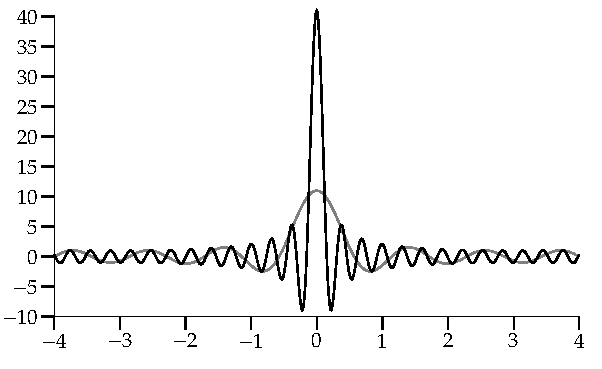
\includegraphics{figures/approxdeltas}
\caption{Plot of $D_N(x)$ for $N=5$ (gray) and $N=20$
(black).\label{fig:approxdeltas}}
\end{myfigureht}

The central peak gets taller and taller as $N$ gets larger,
and the side peaks stay small.
We are convolving (again) with
\emph{approximate delta functions}\index{approximate delta function},
although these functions have
all these oscillations away from zero.  The oscillations on the side do not go away
but they are eventually so fast that we expect the integral to just sort of
cancel itself out there.
Overall, we expect that
$s_N(f)$ goes to $f$.  Things are not always simple,
but under some conditions on $f$, such a conclusion holds.  For this reason
people write
\begin{equation*}
2\pi \, \delta(x) \sim \sum_{n=\infty}^\infty e^{inx} ,
\end{equation*}
where $\delta$ is the \myquote{delta function} (not really a function),
which is an object that will give something like
\myquote{$\int_{-\pi}^{\pi} f(x-t) \delta(t) \, dt = f(x)$.}
We can think of $D_N(x)$ converging in some sense to $2 \pi\, \delta(x)$.
However, we have not defined (and will not define) what kind of an object the delta function
is, nor what does it mean for it to be a limit of $D_N$ or have a Fourier series.

\subsection{Localization}

If $f$ satisfies a Lipschitz condition at a point, then
the Fourier series converges at that point.

\begin{thm} \label{thm:fourierlocalization}
Let $x$ be fixed and let $f$ be a $2\pi$-periodic function
Riemann integrable on $[-\pi,\pi]$.  Suppose
there exist $\delta > 0$ and $M$ such that
\begin{equation*}
\sabs{f(x+t)-f(x)} \leq M \sabs{t}
\end{equation*}
for all $t \in (-\delta,\delta)$, then
\begin{equation*}
\lim_{N \to \infty} s_N(f;x) = f(x) .
\end{equation*}
\end{thm}

In particular,
if $f$ is continuously
differentiable at $x$,
then we obtain convergence (exercise).
We state an often used version of this corollary.
A function $f \colon [a,b] \to \C$ is
\emph{\myindex{continuous piecewise smooth}}\index{piecewise smooth}
if it is continuous and there exist points
$x_0 = a < x_1 < x_2 < \cdots < x_k = b$
such that $f$ restricted to $[x_j,x_{j+1}]$
is continuously differentiable (up to the endpoints) for all $j$.

\begin{cor} \label{cor:fourierpiecewisesmooth}
Let $f$ be a $2\pi$-periodic function
Riemann integrable on $[-\pi,\pi]$.  Suppose
there exist $x\in \R$ and $\delta > 0$ such that $f$ is continuous piecewise
smooth on $[x-\delta,x+\delta]$, then
\begin{equation*}
\lim_{N \to \infty} s_N(f;x) = f(x) .
\end{equation*}
\end{cor}

The proof of the corollary is left as an exercise.  Let us prove the
theorem.

\begin{proof}[Proof of \thmref{thm:fourierlocalization}]
For all $N$,
\begin{equation*}
\frac{1}{2\pi} \int_{-\pi}^\pi D_N = 1 .
\end{equation*}
Write
\begin{equation*}
\begin{split}
s_N(f;x)-f(x) & =
\frac{1}{2\pi} \int_{-\pi}^\pi f(x-t) D_N(t) \, dt 
-
f(x)
\frac{1}{2\pi} \int_{-\pi}^\pi D_N(t) \, dt
\\
& = 
\frac{1}{2\pi} \int_{-\pi}^\pi \bigl( f(x-t) - f(x) \bigr) D_N(t) \, dt 
\\
& = 
\frac{1}{2\pi} \int_{-\pi}^\pi \frac{f(x-t) - f(x)}{\sin(\nicefrac{t}{2})} \sin\bigl(
(N+\nicefrac{1}{2})t \bigr) \, dt .
\end{split}
\end{equation*}
By the hypotheses,
for small nonzero $t$ we get
\begin{equation*}
\abs{ \frac{f(x-t) - f(x)}{\sin(\nicefrac{t}{2})} }
\leq
\frac{M\sabs{t}}{\sabs{\sin(\nicefrac{t}{2})}} .
\end{equation*}
As $\sin(\theta) = \theta + h(\theta)$ where $\frac{h(\theta)}{\theta} \to
0$ as $\theta \to 0$,
we notice that
$\frac{M\sabs{t}}{\sabs{\sin(\nicefrac{t}{2})}}$ is continuous at the origin
and hence 
$\frac{f(x-t) - f(x)}{\sin(\nicefrac{t}{2})}$ must be bounded near the origin.
As $t=0$ is the only place on $[-\pi,\pi]$ where the denominator vanishes,
it is the only place where there could be a problem.  The function is
also Riemann integrable.  We use a trigonometric identity
\begin{equation*}
\sin\bigl( (N+\nicefrac{1}{2})t \bigr)
=
\cos(\nicefrac{t}{2}) \sin(Nt) + 
\sin(\nicefrac{t}{2}) \cos(Nt) ,
\end{equation*}
so
\begin{multline*}
\frac{1}{2\pi} \int_{-\pi}^\pi \frac{f(x-t) - f(x)}{\sin(\nicefrac{t}{2})} \sin\bigl(
(N+\nicefrac{1}{2})t \bigr) \, dt 
= \\
\frac{1}{2\pi} \int_{-\pi}^\pi
\left( \frac{f(x-t) - f(x)}{\sin(\nicefrac{t}{2})}
\cos (\nicefrac{t}{2}) \right) \sin (Nt) \, dt
+
\frac{1}{2\pi} \int_{-\pi}^\pi \bigl( f(x-t) - f(x) \bigr)
\cos (Nt) \, dt .
\end{multline*}
Now 
$\frac{f(x-t) - f(x)}{\sin(\nicefrac{t}{2})} \cos (\nicefrac{t}{2})$
and
$\bigl( f(x-t) - f(x) \bigr)$ are bounded Riemann integrable functions
and so their Fourier coefficients go to zero by \thmref{thm:bessels}.  So the two
integrals on the right-hand side, which compute the Fourier coefficients
for the real version of the Fourier series go to 0 as $N$ goes to infinity.
This is because $\sin(Nt)$ and $\cos(Nt)$ are also orthonormal systems
with respect to the same inner product.
Hence $s_N(f;x)-f(x)$ goes to 0, that is, $s_N(f;x)$ goes to $f(x)$.
\end{proof}

The theorem also says that convergence depends only on local behavior.

\begin{cor}
Suppose $f$ is a $2\pi$-periodic function, Riemann integrable on $[-\pi,\pi]$.
If $J$ is an open interval and $f(x) = 0$ for all $x \in J$,
then $\lim\, s_N(f;x) = 0$ for all $x \in J$.

In particular, if $f$ and $g$ are $2\pi$-periodic functions,
Riemann integrable on $[-\pi,\pi]$, $J$ an open interval, and $f(x) = g(x)$
for all $x \in J$, then for all $x \in J$,
the sequence
$\bigl\{ s_N(f;x) \bigr\}$ converges if and only if $\bigl\{ s_N(g;x) \bigr\}$ converges.
\end{cor}

That is, convergence at $x$ is only dependent on the values of the function
near $x$.  To prove the first claim, take $M=0$ in the theorem.
The \myquote{In particular} follows by considering the function $f-g$, which
is zero on $J$ and $s_N(f-g) = s_N(f) - s_N(g)$.
On the other hand, we have seen that the rate of convergence,
that is how fast does $s_N(f)$
converge to $f$, depends on global behavior of the function.

There is a subtle difference between the corollary and what can be
achieved by the \hyperref[thm:SWcomplex]{Stone--Weierstrass theorem}.
%By Stone--Weierstrass, 
Any continuous function on $[-\pi,\pi]$ can be uniformly approximated
by trigonometric polynomials, but these trigonometric polynomials need
not be the partial sums $s_N$.

\subsection{Parseval's theorem}

Finally,
convergence always happens in the $L^2$ sense and
operations on the (infinite) vectors of
Fourier coefficients are the same as the operations using the integral
inner product.

\begin{samepage}
\begin{thm}[Parseval\footnote{%
Named after the French mathematician
\href{https://en.wikipedia.org/wiki/Marc-Antoine_Parseval}{Marc-Antoine
Parseval}
(1755--1836).}] \index{Parseval's theorem}
Let $f$ and $g$ be $2\pi$-periodic functions, Riemann integrable 
on $[-\pi,\pi]$
with
\begin{equation*}
f(x) \sim
\sum_{n=-\infty}^\infty c_n \,e^{inx}
\qquad \text{and} \qquad
g(x) \sim
\sum_{n=-\infty}^\infty d_n \,e^{inx} .
\end{equation*}
Then
\begin{equation*}
\lim_{N\to\infty} \snorm{f-s_N(f)}_2^2 = 
\lim_{N\to\infty}
\frac{1}{2\pi}
\int_{-\pi}^\pi
\sabs{f(x)-s_N(f;x)}^2 \, dx
=0 .
\end{equation*}
Also
\begin{equation*}
\langle f , g \rangle =
\frac{1}{2\pi}
\int_{-\pi}^\pi
f(x) \overline{g(x)}\, dx
=
\sum_{n=-\infty}^\infty c_n \overline{d_n} ,
\end{equation*}
and
\begin{equation*}
\snorm{f}_2^2
=
\frac{1}{2\pi}
\int_{-\pi}^\pi
\sabs{f(x)}^2 \, dx
=
\sum_{n=-\infty}^\infty \sabs{c_n}^2.
\end{equation*}
\end{thm}
\end{samepage}

\begin{proof}
There exists (exercise)
a continuous $2\pi$-periodic function $h$ such that
\begin{equation*}
\snorm{f-h}_2 < \epsilon .
\end{equation*}
Via \hyperref[thm:SWcomplex]{Stone--Weierstrass},
approximate $h$ with a trigonometric polynomial
uniformly.  That is, there is a trigonometric polynomial $P(x)$
such that
$\sabs{h(x) - P(x)} < \epsilon$ for all $x$.
Hence
\begin{equation*}
\snorm{h-P}_2
=
\sqrt{
\frac{1}{2\pi}
\int_{-\pi}^{\pi}
\sabs{h(x)-P(x)}^2
\,
dx
}
\leq \epsilon.
\end{equation*}
If $P$ is of degree $N_0$, then for all $N \geq N_0$
\begin{equation*}
\snorm{h-s_N(h)}_2 \leq \snorm{h-P}_2 \leq \epsilon ,
\end{equation*}
as $s_N(h)$ is the best approximation for $h$ in $L^2$ (\thmref{thm:l2bestapprox}).
By the inequality leading up to Bessel, we have
\begin{equation*}
\snorm{s_N(h)-s_N(f)}_2
=
\snorm{s_N(h-f)}_2
\leq
\snorm{h-f}_2 \leq \epsilon .
\end{equation*}
The $L^2$ norm satisfies the triangle inequality (exercise).
Thus, for all $N \geq N_0$,
\begin{equation*}
\snorm{f-s_N(f)}_2
\leq
\snorm{f-h}_2
+
\snorm{h-s_N(h)}_2
+
\snorm{s_N(h)-s_N(f)}_2
\leq 3\epsilon .
\end{equation*}
Hence, the first claim follows.

Next,
\begin{equation*}
\langle s_N(f) , g \rangle
=
\frac{1}{2\pi}
\int_{-\pi}^\pi
s_N(f;x) \overline{g(x)} \, dx
=
\sum_{k=-N}^N
c_k 
\frac{1}{2\pi}
\int_{-\pi}^\pi
e^{ikx}
\overline{g(x)} \, dx
=
\sum_{k=-N}^N
c_k 
\overline{d_k} .
\end{equation*}
We need the Schwarz (or Cauchy--Schwarz or Cauchy--Bunyakovsky--Schwarz)
inequality, that is,
\begin{equation*}
{\abs{\int_a^b f\bar{g}}}^2
\leq
\left( \int_a^b \sabs{f}^2 \right)
\left( \int_a^b \sabs{g}^2 \right) .
\end{equation*}
This is left as an exercise.  The proof is not really
different from the finite-dimensional version.
So
\begin{equation*}
\begin{split}
\abs{\int_{-\pi}^\pi f\bar{g} - \int_{-\pi}^\pi s_N(f)\bar{g}}
& =
\abs{\int_{-\pi}^\pi (f- s_N(f))\bar{g}} \\
%& \leq
%\int_{-\pi}^\pi \sabs{f- s_N(f)}\, \sabs{g} \\
& \leq
{\left(\int_{-\pi}^\pi \sabs{f- s_N(f)}^2 \right)}^{1/2}
{\left( \int_{-\pi}^\pi \sabs{g}^2 \right)}^{1/2} .
\end{split}
\end{equation*}
The right-hand side goes to 0 as $N$ goes to infinity by the first
claim of the theorem.
That is, as $N$ goes to infinity, $\langle s_N(f),g \rangle$
goes to $\langle f,g \rangle$, and
the second claim is proved.  The last claim in the theorem follows by using
$g=f$.
\end{proof}

\subsection{Exercises}

\begin{exercise}
Consider the Fourier series
\begin{equation*}
\sum_{n=1}^\infty \frac{1}{2^n} \sin(2^n x) .
\end{equation*}
Show that the series converges uniformly and absolutely to a continuous
function.  Note: This is another example of a nowhere differentiable
function (you do not have to prove that)\footnote{%
See
G.\ H.\ Hardy, \emph{Weierstrass's Non-Differentiable Function},
Transactions of the American Mathematical Society,
\textbf{17}, No.\ 3 (Jul., 1916), pp.\ 301--325.}.
See \figureref{fig:fourierserweier}.
\begin{myfigureht}
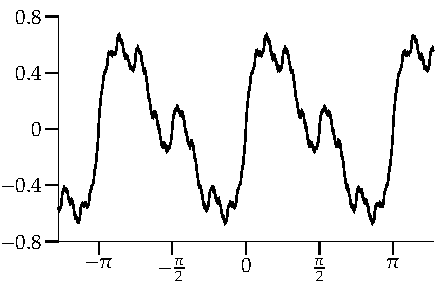
\includegraphics{figures/fourierserweier}
\caption{Plot of 
$\sum_{n=1}^\infty \frac{1}{2^n} \sin(2^n x)$.\label{fig:fourierserweier}}
\end{myfigureht}
\end{exercise}

\begin{exercise}
Suppose that a $2\pi$-periodic function that is Riemann integrable
on $[-\pi,\pi]$, and such that $f$ is continuously differentiable
on some open interval $(a,b)$.  Prove that
for every $x \in (a,b)$, we have $\lim\limits_{N\to\infty} s_N(f;x) = f(x)$.
\end{exercise}

\begin{exercise}
Prove \corref{cor:fourierpiecewisesmooth}, that is,
suppose a $2\pi$-periodic function is continuous piecewise
smooth near a point $x$, then $\lim\limits_{N\to\infty} s_N(f;x) = f(x)$.  Hint: See the previous
exercise.
\end{exercise}

\begin{exercise}
Given a $2\pi$-periodic function $f \colon \R \to \C$ Riemann integrable on
$[-\pi,\pi]$,
and $\epsilon > 0$.
Show that there exists a continuous $2\pi$-periodic function $g \colon \R
\to \C$ such that $\snorm{f-g}_2 < \epsilon$.
\end{exercise}

\begin{exercise}
Prove the Cauchy--Bunyakovsky--Schwarz inequality
for Riemann integrable functions:
\begin{equation*}
{\abs{\int_a^b f\bar{g}}}^2
\leq
\left( \int_a^b \sabs{f}^2 \right)
\left( \int_a^b \sabs{g}^2 \right) .
\end{equation*}
\end{exercise}

\begin{exercise}
Prove the $L^2$ triangle inequality 
for Riemann integrable functions on $[-\pi,\pi]$:
\begin{equation*}
\snorm{f+g}_2 \leq \snorm{f}_2 + \snorm{g}_2 .
\end{equation*}
\end{exercise}

\begin{exercise}
\pagebreak[3]
Suppose for some $C$ and $\alpha > 1$, we have
a real sequence $\{ a_n \}$ with
$\abs{a_n} \leq \frac{C}{n^\alpha}$ for all $n$.
Let
\begin{equation*}
g(x) := \sum_{n=1}^\infty a_n \sin(n x) .
\end{equation*}
\begin{enumerate}[a)]
\item
Show that $g$ is continuous.
\item
Formally (that is, suppose you can differentiate under the sum)
find a solution (formal solution, that is, do not yet worry about convergence)
to the differential equation
\begin{equation*}
y''+ 2 y = g(x)
\end{equation*}
of the form
\begin{equation*}
y(x) = \sum_{n=1}^\infty b_n \sin(n x) .
\end{equation*}
\item
Then show that this solution $y$ is twice continuously differentiable,
and in fact solves the equation.
\end{enumerate}
\end{exercise}

\begin{exercise}
Let $f$ be a $2\pi$-periodic  function such
that $f(x) = x$ for $0 < x < 2\pi$.
Use Parseval's theorem to find
\begin{equation*}
\sum_{n=1}^\infty \frac{1}{n^2} = \frac{\pi^2}{6} .
\end{equation*}
\end{exercise}

\begin{exercise}
Suppose that $c_n = 0$ for all $n < 0$ and $\sum_{n=0}^\infty \sabs{c_n}$
converges.  Let $\D := B(0,1) \subset \C$ be the unit disc,
and $\overline{\D} = C(0,1)$ be the closed unit disc.
Show that there exists a continuous function
$f \colon \overline{\D} \to \C$ that is analytic on $\D$
and such that on the boundary of $\D$ we have
$f(e^{i\theta}) = \sum_{n=0}^\infty c_n e^{i\theta}$.\\
Hint: If $z=re^{i\theta}$, then $z^n = r^n e^{in\theta}$.
\end{exercise}

\begin{exercise}
Show that
\begin{equation*}
\sum_{n=1}^\infty e^{-1/n} \sin(n x)
\end{equation*}
converges to an infinitely differentiable function.
\end{exercise}

\begin{exercise}
Let $f$ be a $2\pi$-periodic function
such that $f(x) = f(0) + \int_0^x g$
for a function $g$ that is Riemann integrable on every interval.
Suppose
\begin{equation*}
f(x) \sim
\sum_{n=-\infty}^\infty c_n \,e^{inx} .
\end{equation*}
Show that there exists a $C > 0$ such that
$\sabs{c_n} \leq \frac{C}{\sabs{n}}$.
\end{exercise}

\begin{exercise}
\leavevmode
\begin{enumerate}[a)]
\item
Let $\varphi$ be the $2\pi$-periodic function 
defined by $\varphi(x) := 0$ if $x \in (-\pi,0)$,
and $\varphi(x) := 1$ if $x \in (0,\pi)$,
letting $\varphi(0)$ and $\varphi(\pi)$ be arbitrary.  Show
that $\lim \, s_N(\varphi;0) = \nicefrac{1}{2}$.
\item
Let $f$ be a $2\pi$-periodic function
Riemann integrable on $[-\pi,\pi]$, 
$x \in \R$, $\delta > 0$, and
there are continuously differentiable
$g \colon [x-\delta,x] \to \C$
and $h \colon [x,x+\delta] \to \C$
where $f(t) = g(t)$ for all $t \in [x-\delta,x)$
and
where $f(t) = h(t)$ for all $t \in (x,x+\delta]$.
Then
$\lim\, s_N(f;x) = \frac{g(x)+h(x)}{2}$, or in other words:
\begin{equation*}
\lim_{N \to \infty} s_N(f;x) =
\frac{1}{2}
\left(
\lim_{t \to x^-} f(t) +
\lim_{t \to x^+} f(t)
\right) .
\end{equation*}
\end{enumerate}
\end{exercise}



%%%%%%%%%%%%%%%%%%%%%%%%%%%%%%%%%%%%%%%%%%%%%%%%%%%%%%%%%%%%%%%%%%%%%%%%%%%%%%
%%%%%%%%%%%%%%%%%%%%%%%%%%%%%%%%%%%%%%%%%%%%%%%%%%%%%%%%%%%%%%%%%%%%%%%%%%%%%%
%%%%%%%%%%%%%%%%%%%%%%%%%%%%%%%%%%%%%%%%%%%%%%%%%%%%%%%%%%%%%%%%%%%%%%%%%%%%%%

\cleardoublepage  
\phantomsection
\addcontentsline{toc}{chapter}{Further Reading}
\markboth{FURTHER READING}{FURTHER READING}
\begin{bibchapter}[Further Reading]
\begin{biblist}[\normalsize]

\bib{Rosenlicht}{book}{
   author={Rosenlicht, Maxwell},
   title={Introduction to Analysis},
   note={Reprint of the 1968 edition},
   publisher={Dover Publications Inc.},
   place={New York},
   date={1986},
   pages={viii+254},
   isbn={0-486-65038-3},
}

\bib{Rudin:baby}{book}{
   author={Rudin, Walter},
   title={Principles of Mathematical Analysis},
   edition={3},
   note={International Series in Pure and Applied Mathematics},
   publisher={McGraw-Hill Book Co.},
   place={New York},
   date={1976},
   pages={x+342},
}

\bib{Trench}{book}{
   author={Trench, William F.},
   title={Introduction to Real Analysis},
   year={2003},
   publisher={Pearson Education},
   note={\url{http://ramanujan.math.trinity.edu/wtrench/texts/TRENCH_REAL_ANALYSIS.PDF}},
}



\end{biblist}
\end{bibchapter}

%%%%%%%%%%%%%%%%%%%%%%%%%%%%%%%%%%%%%%%%%%%%%%%%%%%%%%%%%%%%%%%%%%%%%%%%%%%%%%
%%%%%%%%%%%%%%%%%%%%%%%%%%%%%%%%%%%%%%%%%%%%%%%%%%%%%%%%%%%%%%%%%%%%%%%%%%%%%%
%%%%%%%%%%%%%%%%%%%%%%%%%%%%%%%%%%%%%%%%%%%%%%%%%%%%%%%%%%%%%%%%%%%%%%%%%%%%%%

\cleardoublepage
\phantomsection
\addcontentsline{toc}{chapter}{\indexname}  
\microtypesetup{protrusion=false}
\printindex
\microtypesetup{protrusion=true}

%%%%%%%%%%%%%%%%%%%%%%%%%%%%%%%%%%%%%%%%%%%%%%%%%%%%%%%%%%%%%%%%%%%%%%%%%%%%%%
%%%%%%%%%%%%%%%%%%%%%%%%%%%%%%%%%%%%%%%%%%%%%%%%%%%%%%%%%%%%%%%%%%%%%%%%%%%%%%
%%%%%%%%%%%%%%%%%%%%%%%%%%%%%%%%%%%%%%%%%%%%%%%%%%%%%%%%%%%%%%%%%%%%%%%%%%%%%%

%
% automake on glossaries doesn't work if the index is before the glossary.
% That's why the List of Notation is last, no other reason.  Problem is
% that printindex does a clearpage which screws up the delayed write18
% that glossaries sets up
%

\begingroup
\renewcommand{\pagelistname}{Page}
\setglossarystyle{long3colheader}
% correctly set up with cellspace
\renewenvironment{theglossary}%
  {\setlength\cellspacetoplimit{4pt}
   \setlength\cellspacebottomlimit{4pt}
   \setlength\LTleft{0pt}
   \setlength\LTright{0pt}
   \markboth{LIST OF NOTATION}{LIST OF NOTATION}
   \begin{longtable}{Sl @{\extracolsep{\fill}} Sl @{\extracolsep{\fill}} Sl}}%
  {\end{longtable}}%
\microtypesetup{protrusion=false}
\printglossary[title=List of Notation] 
\microtypesetup{protrusion=true}
\endgroup


\end{document}
